\documentclass[12pt, a4paper, twoside, openright]{report}
\usepackage{emptypage}
\raggedbottom


\usepackage{pdfpages}

% --- LINGUA E FONT ---
\usepackage[english]{babel}
\usepackage[utf8]{inputenc}
\usepackage[T1]{fontenc}
\usepackage{mathptmx} % Imposta il font Times New Roman

% --- MARGINI (Direttive Uni: 2.5 cm ovunque) ---
\usepackage[margin=2.5cm]{geometry}

% --- INTERLINEA (Direttive Uni: 1.5) ---
\usepackage{setspace}
\onehalfspacing

% --- PACCHETTI GRAFICI E MATEMATICI ---
\usepackage{graphicx} % Per inserire le immagini
\usepackage{float}    % Per bloccare le immagini
\usepackage{amsmath}  % Per le formule matematiche avanzate
\usepackage{amssymb}

% --- PACCHETTI PER TABELLA ---
\usepackage{tabularx}
\usepackage{booktabs}

% --- PACCHETTI PER CODICE E COLORI ---
\usepackage{xcolor}
\usepackage{listings}

% Definizione Colori
\definecolor{backcolour}{rgb}{0.96, 0.96, 0.94} % Beige chiaro
\definecolor{commentgreen}{rgb}{0.0, 0.6, 0.0}
\definecolor{stringpurple}{rgb}{0.58, 0.0, 0.82}
\definecolor{keywordblue}{rgb}{0.0, 0.0, 0.8}
\definecolor{bashkeyword}{rgb}{0.0, 0.4, 0.5} 
\definecolor{yamlkey}{rgb}{0.8, 0.1, 0.1}       % Rosso scuro per le chiavi YAML

% Configurazione globale di base
\lstset{
    backgroundcolor=\color{backcolour},   
    commentstyle=\color{commentgreen},
    numberstyle=\tiny\color{gray},
    basicstyle=\ttfamily\footnotesize,
    breaklines=true,                 
    captionpos=b,                    
    keepspaces=true,                 
    numbers=left,                    
    numbersep=10pt,                  
    frame=single,                    % Bordo attorno al codice
    rulecolor=\color{lightgray},     % Colore del bordo (grigio chiaro)
    showspaces=false,                
    showstringspaces=false,
    showtabs=false,                  
    tabsize=2
}

% --- DEFINIZIONE CUSTOM PER YAML ---
\lstdefinelanguage{yaml}{
  keywords={true, false, null, y, n, True, False},
  keywordstyle=\color{keywordblue}\bfseries,
  comment=[l]{\#},
  commentstyle=\color{commentgreen}\ttfamily,
  stringstyle=\color{stringpurple}\ttfamily,
  moredelim=**[l][\color{yamlkey}\bfseries]{:},  
  morestring=[b]',
  morestring=[b]"
}

% --- STILI SPECIFICI PER LINGUAGGIO ---
\lstdefinestyle{mybash}{
    language=bash,
    keywordstyle=\color{bashkeyword}\bfseries,
    stringstyle=\color{stringpurple},
    %Comandi linux e ROS da colorare:
    morekeywords={mkdir, cat, echo, export, exec, chmod, sed, ros2, until, grep, sleep, done}
}

\lstdefinestyle{myxml}{
    language=XML,
    keywordstyle=\color{keywordblue}\bfseries,
    stringstyle=\color{stringpurple},
    %Tag custom di ROS/Gazebo e XACRO:
    morekeywords={plugin, ros, namespace, remapping, update_rate, xacro:if, xacro:include}
}

\lstdefinestyle{mypython}{
    language=Python,
    keywordstyle=\color{keywordblue}\bfseries,
    stringstyle=\color{stringpurple},
    % Eventuali classi custom python da evidenziare
    morekeywords={rclpy, Node, ExecuteProcess, LaunchDescription, DeclareLaunchArgument}
}

\lstdefinestyle{myyaml}{
    language=yaml
}

% --- SETUP BIBLIOGRAFIA ---
\usepackage[backend=biber, style=ieee]{biblatex} 
\addbibresource{Thesis Robotics.bib} 

% --- SETUP LINK CLICCABILI  ---
\usepackage[colorlinks=true, citecolor=black, linkcolor=black, urlcolor=blue]{hyperref}

% --- SETUP IMMAGINI  ---
\usepackage{tikz}
\usetikzlibrary{positioning, arrows.meta, shapes.geometric}

% --- PER IMMAGINI IN ALTO  ---
\makeatletter
\setlength{\@fptop}{0pt}
\makeatother

\begin{document}

% ==========================================
% FRONTESPIZIO
% ==========================================
\pagenumbering{roman} 

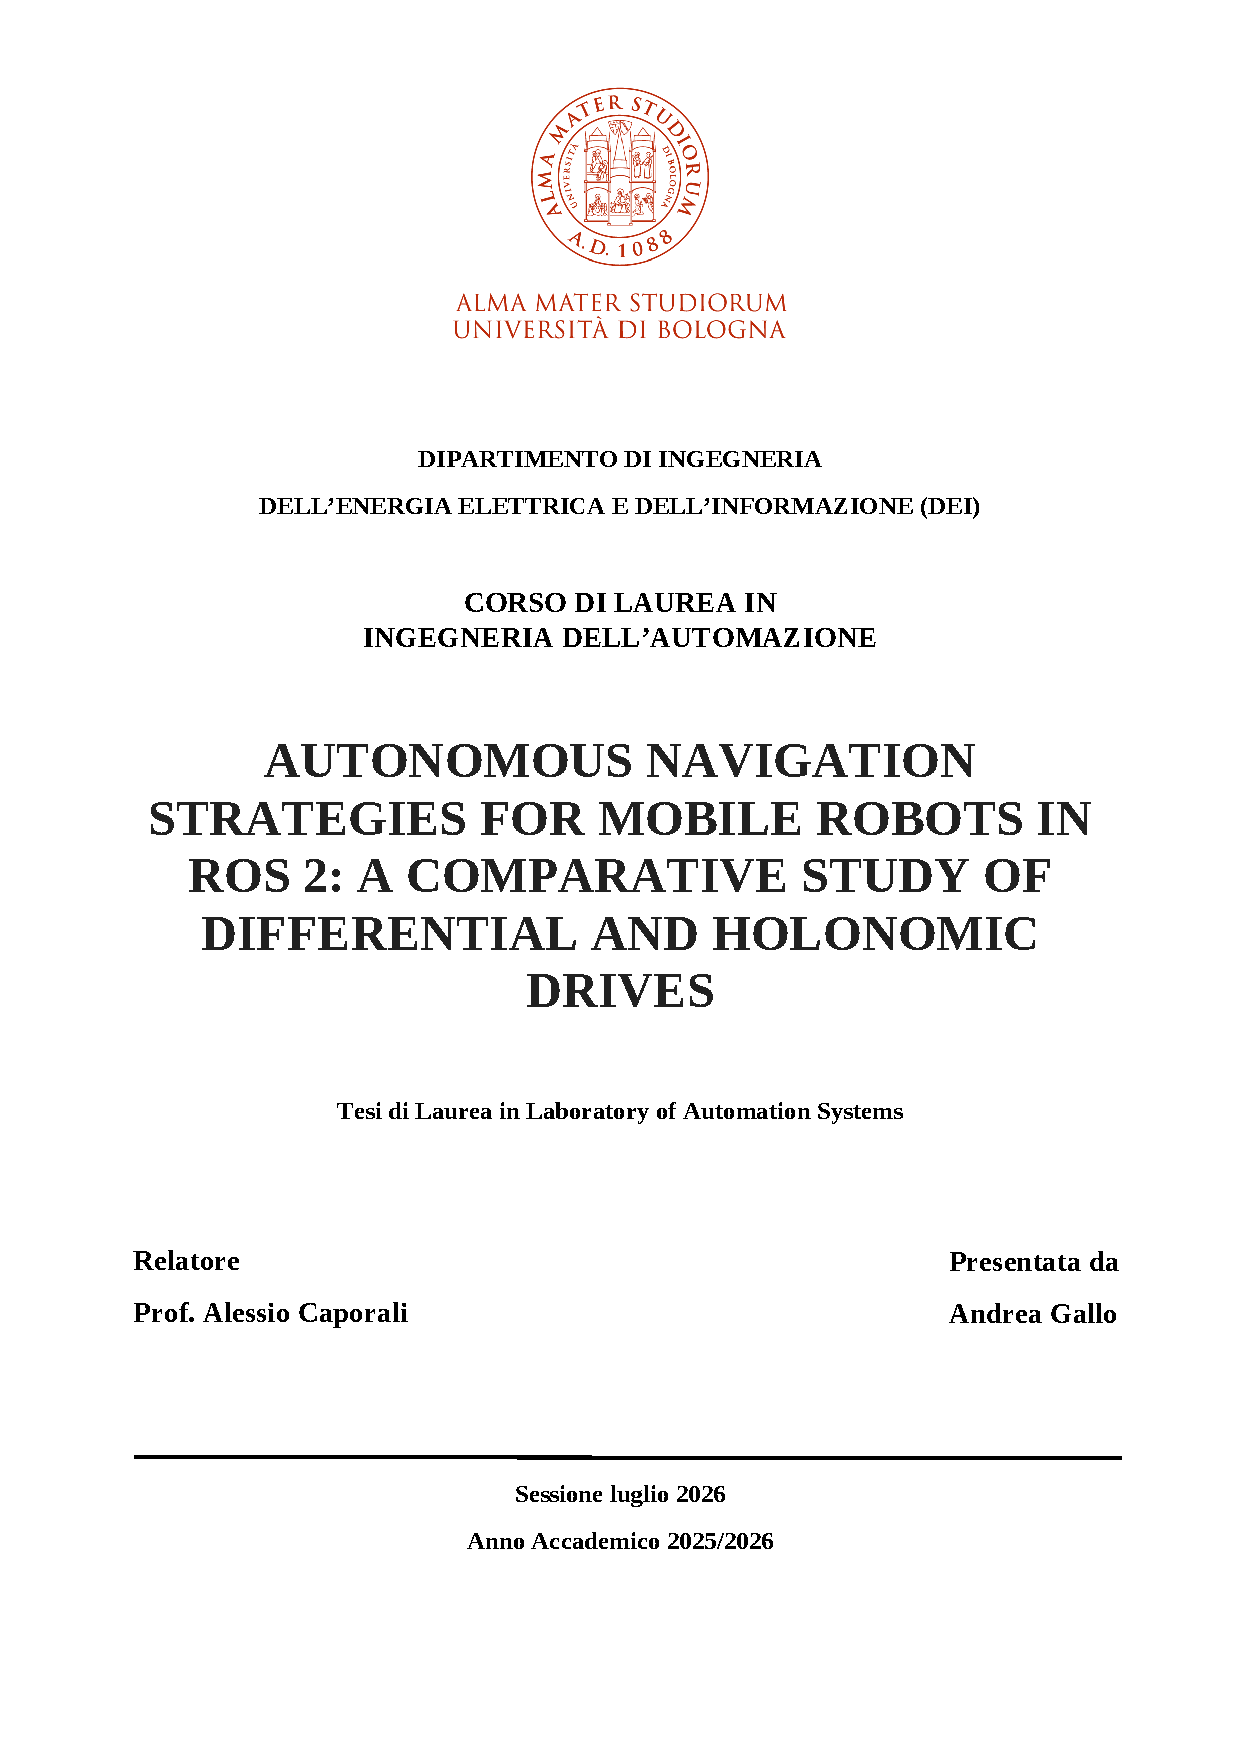
\includepdf[pages=1]{Frontespizio Tesi_compilato.pdf}
\clearpage
\thispagestyle{empty}
\null
\clearpage

% ==========================================
% ABSTRACT E INDICE
% ==========================================
% Numerazione romana per le pagine dell'indice

\cleardoublepage
\chapter*{Abstract}
Autonomous Mobile Robots are increasingly deployed in complex indoor environments, raising the question of which kinematic drive---differential or holonomic---is best suited for autonomous navigation. Standard open-source frameworks such as ROS~2 Nav2, however, exhibit an inherent ``differential bias'': by heavily penalizing lateral motion, they force holonomic bases into sub-optimal, pseudo-differential behaviors. This thesis presents an equitable comparison between a differential drive (TIAGo PMB2) and a holonomic drive (TIAGo OmniBase) in ROS~2. To enable a fair benchmark, the Nav2 stack was profoundly reconfigured---tuning the local planner critics and kinematic constraints---to suppress this bias and unlock true omnidirectional motion. The platforms were evaluated in Gazebo across two pipelines: directed waypoint navigation under varying topological challenges, and autonomous frontier-based exploration with online SLAM. To prevent estimation noise from skewing the results, all spatial metrics were computed offline from absolute ground-truth poses. The results reveal a clear kinematic trade-off. The holonomic drive shows decisive planning robustness in confined spaces, achieving zero global-planning failures and negotiating sharp corners far faster through lateral strafing. Conversely, the differential drive proves faster and more efficient in open areas and wall-following, thanks to its circular footprint, but suffers severe planning fragility and frequent recoveries in cluttered passages. As the two bases are actuated by different simulation plugins, these differences are framed at the level of navigation strategy rather than physical execution. The findings yield concrete engineering guidelines, showing that the optimal choice is dictated by environmental density and operational constraints such as mobile manipulation.

\cleardoublepage
\chapter*{Sommario}
I Robot Mobili Autonomi sono sempre più impiegati in ambienti indoor complessi, sollevando il problema di quale cinematica---differenziale o olonoma---sia la più adatta per la navigazione autonoma. Tuttavia, i framework open-source standard come ROS~2 Nav2 presentano un intrinseco ``bias differenziale'': penalizzando fortemente il moto laterale, costringono le basi olonome a comportamenti sub-ottimali. Questa tesi presenta un confronto equo tra una base differenziale (TIAGo PMB2) e una olonoma (TIAGo OmniBase) in ROS~2. Per un benchmark corretto, lo stack Nav2 è stato profondamente riconfigurato---modificando i critici del \textit{local planner} e i vincoli cinematici---per sopprimere tale bias e sbloccare il reale moto omnidirezionale. Le piattaforme sono state valutate in Gazebo su due scenari: navigazione a waypoint con sfide topologiche di varia difficoltà ed esplorazione autonoma \textit{frontier-based} con SLAM online. Per escludere il rumore di stima, tutte le metriche spaziali sono state calcolate offline dalla \textit{ground truth} assoluta. I risultati mostrano un chiaro \textit{trade-off}. La base olonoma garantisce una robustezza di pianificazione decisamente superiore negli spazi ristretti, azzerando i fallimenti del \textit{global planner} e superando le curve strette molto più rapidamente tramite il moto laterale. Al contrario, la base differenziale è più veloce ed efficiente in aree aperte e nel \textit{wall-following}, grazie all'ingombro circolare, ma mostra una forte fragilità di pianificazione e continue \textit{recovery} in ambienti congestionati. Poiché le due basi sono attuate da plugin di simulazione differenti, tali differenze vanno intese a livello di strategia di navigazione più che di esecuzione fisica. Lo studio fornisce linee guida pratiche, dimostrando che la scelta ottimale dipende dalla densità dell'ambiente e da vincoli operativi come la manipolazione mobile.



\tableofcontents
\cleardoublepage

\pagenumbering{arabic} % Torna alla numerazione normale per le pagine dei capitoli



% ==========================================
% INSERIMENTO CAPITOLI
% ==========================================
%!TeX root = ../main.tex

% ==========================================
% CHAPTER 1: INTRODUCTION
% ==========================================
\chapter{Introduction}
\label{ch:intro}

\section{Context and Motivation}

In recent years, the deployment of Autonomous Mobile Robots (AMRs) has expanded significantly beyond highly controlled industrial environments, such as factories and automated warehouses. Today, AMRs are increasingly integrated into complex, unstructured, and dynamic indoor settings, ranging from hospitals and retail stores to domestic environments \cite{siegwart2004introduction}. Unlike traditional industrial floors, domestic and service environments present unique navigational challenges: navigating through narrow doorways, avoiding unpredictable dynamic obstacles (such as humans and pets), and maintaining a stable sensor line-of-sight during complex manoeuvres. Navigating such spaces safely and efficiently imposes stringent requirements on both the physical manoeuvrability of the robotic platform and the robustness of its software control architecture.

Historically, the differential drive kinematics has been the industry standard for indoor mobile robots due to its mechanical simplicity, reliability, and ease of control \cite{siegwart2004introduction}. However, as derived in Chapter 2, differential drive platforms are strictly bound by non-holonomic constraints. To achieve lateral displacements or navigate sharp corners, a non-holonomic robot must execute a sequence of forward translations and in-place rotations. In heavily constrained environments, these manoeuvres significantly increase the robot's dynamic footprint—or \textit{swept volume}—elevating the risk of collision and reducing the overall fluidity of the navigation. 

To overcome these physical limitations, holonomic platforms, such as those equipped with Mecanum wheels, have been introduced. By granting full 3-degree-of-freedom (3-DOF) planar mobility, holonomic robots can perform instantaneous lateral translations (strafing) without altering their heading. This capability is particularly critical for domestic robots and mobile manipulators, which often need to maintain a continuous line-of-sight with a target or keep a manipulated payload steady while avoiding obstacles.

Despite the hardware readiness of omnidirectional platforms, a critical gap remains in the software infrastructure. Modern open-source navigation frameworks, most notably the Navigation 2 (Nav2) stack within the Robot Operating System 2 (ROS 2), have been historically designed and optimized around differential and Ackermann kinematic models \cite{macenski_marathon_2020}. Consequently, deploying a holonomic base using default navigation algorithms often results in sub-optimal, "pseudo-differential" behaviors, where the system fails to exploit the available lateral degrees of freedom. 

The motivation for this thesis stems from the necessity to bridge this gap between hardware capabilities and software limitations. A fair and scientifically rigorous comparison between differential and holonomic drives cannot be achieved out-of-the-box. It requires a profound architectural tuning of the local planning algorithms to actively suppress the differential bias and unlock true omnidirectional capabilities. Therefore, this work aims to systematically reconfigure the ROS 2 navigation stack for both paradigms, providing a standardized baseline to evaluate how the underlying kinematics influence exploration strategies, path execution, and overall operational efficiency in complex indoor scenarios.

\section{State of the Art on Mobile Robot Locomotion}

The scientific literature and industrial applications surrounding mobile robot locomotion are broadly polarized into two primary paradigms: non-holonomic (differential) and holonomic (omnidirectional) systems.

From a mechanical standpoint, differential drive platforms dominate due to their reliability, simplicity, and power efficiency, though they suffer from limited manoeuvrability in cluttered environments \cite{pal_blog_omni_diff}. Conversely, platforms equipped with Mecanum wheels allow instantaneous translation in any planar direction, maximizing manoeuvrability at the cost of reduced energy efficiency and increased sensitivity to floor irregularities due to passive rollers \cite{taheri_kinematic_2015, reque_mechatronics_2021, yepez-figueroa_design_2025}.

While the hardware differences are well documented, the algorithmic implications of deploying these kinematic models present a significant challenge. Autonomous navigation frameworks, such as ROS 2 Nav2 \cite{macenski_marathon_2020}, divide the navigation task into global path planning and local trajectory control. Historically, standard local planners—such as the Dynamic Window Approach (DWA)—were mathematically formulated around non-holonomic constraints. Consequently, these planners inherently exhibit a \textit{differential bias}: their objective cost functions heavily penalize trajectories where the robot's heading does not align with the direction of motion. When an omnidirectional robot is deployed using these default configurations, it often exhibits "pseudo-differential" behaviors, rotating unnecessarily rather than exploiting its lateral degrees of freedom.

To address this limitation, recent literature has explored various approaches to holonomic local planning. Several studies have compared standard ROS planners, demonstrating that optimization-based algorithms like the Timed Elastic Band (TEB) often outperform DWA-based approaches on omnidirectional bases by explicitly handling kinematic constraints \cite{imamoglu2023comparison}. Furthermore, to fully leverage omnidirectional capabilities without being constrained by standard Nav2 heuristics, researchers frequently bypass standard software stacks. Advanced implementations increasingly rely on Nonlinear Model Predictive Control (NMPC) or custom non-linear optimization formulations, which design rotationally invariant cost functions to guarantee smooth, pure translational movements (\textit{crab walk}) in narrow spaces \cite{sun2022local}.

Despite these advancements, a significant gap remains in the state of the art for industrial, out-of-the-box deployments. While custom MPC planners excel in specific scenarios, there is a lack of comprehensive benchmarking that evaluates how standard, widely adopted open-source frameworks like Nav2 can be systematically tuned to suppress the differential bias on holonomic hardware. This thesis positions itself within this gap. By utilizing the modular PAL Robotics TIAGo platform \cite{pal_tiago_base, pal_tiago_omnibase}, this study isolates the kinematic variables and provides a reproducible baseline to evaluate how standard Nav2 controllers can be reconfigured to bridge the gap between differential planning heuristics and true holonomic mobility.

\section{Objectives and Contributions of the Thesis}

The primary objective of this thesis is to conduct a comparative analysis of autonomous exploration and navigation strategies between a differential drive robot (TIAGo PMB2) and an omnidirectional robot (TIAGo OmniBase), operating within the ROS 2 Nav2 framework. 

Rather than executing a purely theoretical kinematic analysis, this work focuses on the engineering challenge of deploying both systems in a realistic simulation environment, identifying the software bottlenecks, and tuning the navigation stack to allow a scientifically fair benchmark.

The specific contributions of this thesis are:
\begin{itemize}
    \item \textbf{System Architecture Configuration and Troubleshooting:} The integration and debugging of the ROS 2 workspace for the TIAGo OmniBase, resolving underlying issues in the official simulator packages (e.g., missing TF frames for the odometry and plugin conflicts) to ensure the stability of the Gazebo simulation.
    \item \textbf{Algorithmic Tuning of the Local Planner (DWB):} The critical reconfiguration of the DWB Local Planner's Critics. By actively suppressing the differential bias (such as the \textit{PathAlign} and \textit{GoalAlign} scores) and tuning velocity limits, the holonomic base was successfully forced into a pure translational motion (\textit{crab walk}), maximizing its kinematic advantage in narrow environments.
    \item \textbf{Ground-Truth Based Evaluation:} The development of a robust offline analysis infrastructure. To guarantee an objective evaluation unaffected by odometry drift, the spatial tracking errors, the waypoint positioning errors, and the execution times were computed from absolute Ground Truth poses extracted directly from the Gazebo physics engine. Motion smoothness was quantified separately as the root mean-square of the commanded linear and angular accelerations, obtained by differentiating the velocity commands issued by the navigation stack.
    \item \textbf{Comprehensive Benchmarking and Autonomous Exploration:} The design of a multi-tiered experimental setup. The platforms were first tested through directed waypoint navigation (using the \texttt{NavigateThroughPoses} action) across three specific topological challenges: a straight path, a 90-degree corner, and an obstacle course. Subsequently, both bases were evaluated in a realistic domestic environment using a custom robust frontier-based exploration algorithm. Originally developed during a prior internship, this node was heavily instrumented for this thesis to ensure deterministic and fair comparisons. It introduces advanced navigation heuristics—such as dynamic goal retraction from unknown boundaries, strict wall-clearance filtering, and dynamic goal blacklisting—to prevent planner failures and timeouts. All scenarios were repeated for 5 iterations per base to characterise run-to-run variability (reported as mean and standard deviation).
    \item \textbf{Cross-Paradigm Empirical Findings:} A quantitative characterisation of the trade-offs between the two kinematics, shown to be consistent across both navigation pipelines. The holonomic base leverages lateral motion to track straight paths more closely and to negotiate sharp corners substantially faster---by strafing rather than rotating in place---at the cost of larger deviations from the planned path when cutting corners. More significantly, the differential base exhibits a recurring planning fragility around obstacles, manifesting as repeated global-planner failures, which the holonomic base does not; this same fragility reappears in the autonomous-exploration task, establishing it as a robustness result that is independent of the specific navigation paradigm.
\end{itemize}

\section{Thesis Outline}

The remainder of this thesis is structured as follows:
\begin{itemize}
    \item \textbf{Chapter~\ref{Ch:Kinematic}} establishes the theoretical foundation, detailing the kinematic equations, mobility constraints, and probabilistic motion models for both the differential (PMB2) and omnidirectional (OmniBase) drives.
    \item \textbf{Chapter~\ref{ch:architecture}} describes the system architecture and the ROS 2 Nav2 setup. It highlights the crucial software modifications, the resolution of simulation artifacts, and the parameter tuning required to enable fair omnidirectional navigation.
    \item \textbf{Chapter~\ref{ch:results}} presents the experimental setup and the quantitative analysis of the results. It details the performance of both bases across the three waypoint-based scenarios and the autonomous exploration task, evaluating metrics such as trajectory tracking error, execution time, and motion fluidity.
    \item \textbf{Chapter~\ref{ch:conclusions}} concludes the thesis by summarizing the main empirical findings and translating the experimental results into practical engineering guidelines. It provides clear recommendations on when to deploy a differential or a holonomic drive based on their respective strengths, weaknesses, and operational constraints, ultimately proposing directions for future research and developments.
\end{itemize}


%\clearpage
%\thispagestyle{empty}
%\null
%\clearpage
%!TeX root = ../main.tex

% ==========================================
% CHAPTER 2: KINEMATIC AND PROBABILISTIC MODELS 
% ==========================================
\chapter{Kinematic and Probabilistic Models of Mobile Robots}
\label{Ch:Kinematic}
This chapter establishes the mathematical and theoretical foundations governing the locomotion of the analyzed robotic platforms. Before addressing the software configuration of the navigation stack, it is essential to formally define the physical constraints that dictate how the robot interacts with its environment. The chapter begins by defining the configuration space and the fundamental distinction between holonomic and non-holonomic constraints (Section~\ref{sec:intro_kin}). Subsequently, it derives the direct and inverse kinematics for both the differential drive PMB2 (Section~\ref{sec:diff_model}) and the omnidirectional OmniBase (Section~\ref{sec:omni_model}). Finally, acknowledging that real-world locomotion is inevitably affected by unmodeled physical interactions, Section~\ref{sec:probabilistic_motion_models} introduces the probabilistic motion models, characterizing the distinct odometric noise profiles of both drives. These theoretical principles provide the necessary justification for the infrastructural adaptations and algorithmic tuning detailed in Chapter~\ref{ch:architecture}.

\section{Introduction to Mobile Robot Mobility}
\label{sec:intro_kin}

The study of mobile robot kinematics deals with the mathematical description of motion without considering the forces that cause it. Before analyzing the specific models of the TIAGo robot, it is essential to define the basic concepts of mobility, configuration space, and kinematic constraints.

For a mobile robot operating in a 2D planar environment, its pose (or posture) is uniquely defined by a vector in the configuration space. Typically, this vector is denoted as:
\begin{equation}
    q = \begin{bmatrix} x \\ y \\ \theta \end{bmatrix} \in \mathbb{R}^2 \times S^1
\end{equation}
where $x$ and $y$ represent the Cartesian coordinates of a reference point on the robot chassis, and $\theta$ represents its orientation (heading) with respect to a global reference frame \cite{palli_amr_slides}.

The mobility of a robot is strictly determined by the mechanical design of its wheels and how they interact with the ground. Assuming the ideal condition of pure rolling without slipping, each wheel imposes specific kinematic constraints on the robot's motion. In mobile robotics, we generally distinguish between two main categories of constraints:

\begin{itemize}
    \item \textbf{Holonomic constraints:} These are constraints on the position (or configuration) variables. A robot is considered holonomic if its controllable degrees of freedom (DOFs) are equal to the total degrees of freedom of its configuration space. In a planar environment, a holonomic robot can instantaneously move in any direction $(x, y)$ while independently changing its orientation $\theta$.
    
    \item \textbf{Non-holonomic constraints:} These are differential constraints on the robot's velocities that cannot be integrated into finite position constraints. They limit the instantaneous directions in which the robot can move, but they do not reduce the overall reachable configuration space. A classic example is a standard car, which can be parked anywhere but cannot instantaneously move sideways.
\end{itemize}

The two bases of the TIAGo robot analyzed in this thesis perfectly represent these two opposite categories: the standard PMB2 base is a non-holonomic system, whereas the OmniBase is a fully holonomic system. The following sections will mathematically detail the kinematic implications of these designs.


\section{Differential Drive Model (TIAGo PMB2)}
\label{sec:diff_model}

The default mobile base of the TIAGo robot is the PMB2 (PAL Mobile Base 2), which employs a differential drive locomotion system \cite{pal_tiago_base}. According to the manufacturer, this configuration provides high agility in standard indoor environments with a circular footprint, making it ideal for general-purpose navigation tasks \cite{pal_blog_omni_diff}. The configuration consists of two independently actuated, coaxial wheels located at the sides of the robot, supplemented by four passive caster wheels for mechanical stability.

\subsection{Physical Configuration}

Let us define the geometric parameters of the PMB2 base (Figure~\ref{fig:diff_drive_model}):
\begin{itemize}
    \item $r$: radius of the driven wheels;
    \item $d$: wheelbase, defined as the distance between the centers of the two driven wheels;
    \item $\omega_R, \omega_L$: angular velocities of the right and left wheel, respectively.
\end{itemize}

% --- INIZIO INSERIMENTO IMMAGINE ---
    \begin{figure}[htbp]
        \centering
        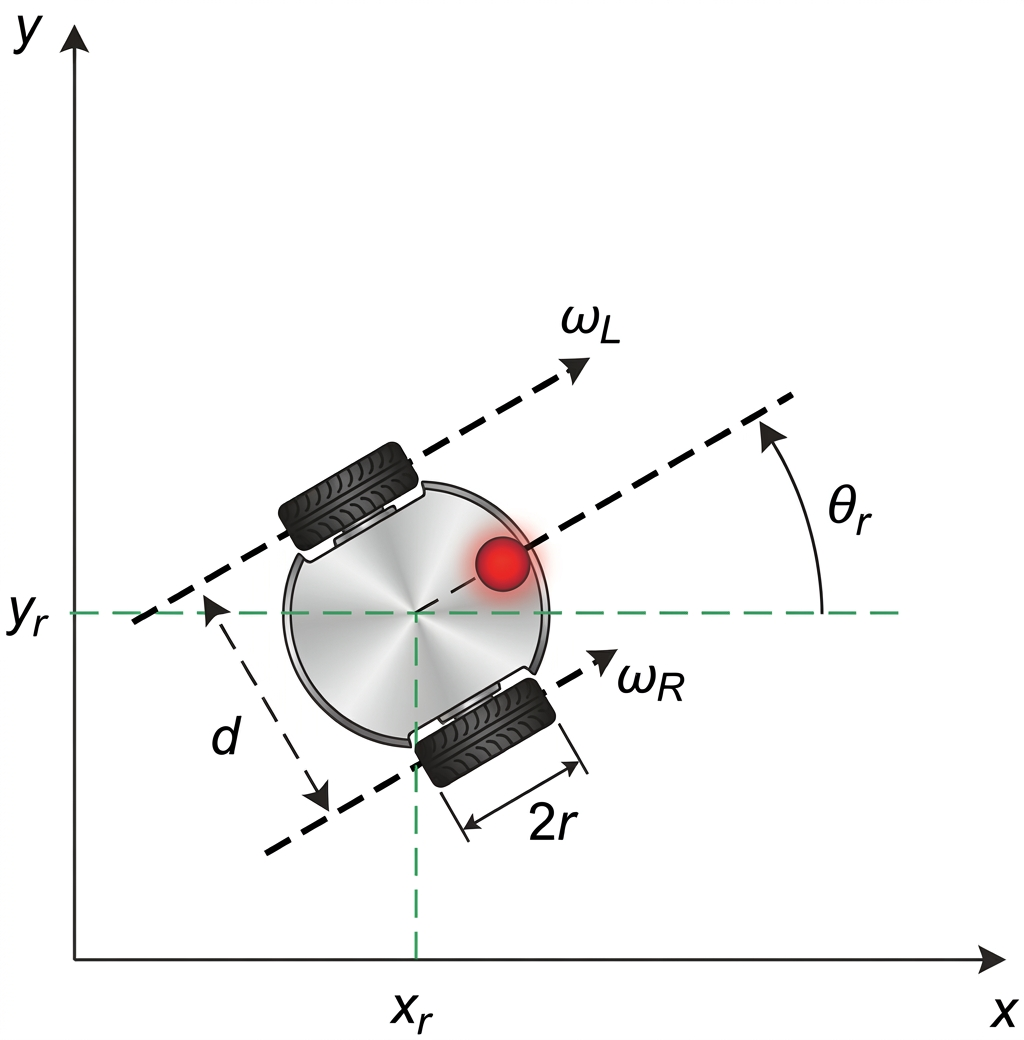
\includegraphics[width=0.5\textwidth]{images/Ch2/Modello unicycle robot.jpg}
        \caption{Kinematic model of a differential drive robot (Image adapted from \cite{palli_amr_slides}).}
        \label{fig:diff_drive_model}
    \end{figure}
% --- FINE INSERIMENTO IMMAGINE ---

\subsection{Direct and Inverse Kinematics}

Because the differential drive is kinematically equivalent to a single steerable wheel located at the midpoint of the wheel axle (the red circle), it can be mathematically described by the \emph{unicycle kinematic model} \cite{palli_amr_slides}.

By controlling the angular velocities of the two independent wheels, it is possible to govern both the translational velocity $v$ and the rotational velocity $\omega$ of the robot. The \emph{Direct Kinematics} equations mapping the individual wheel velocities to the robot's local velocities are:
\begin{equation}
    v = \frac{r}{2} (\omega_R + \omega_L) \quad\quad, \quad \quad \omega = \frac{r}{d} (\omega_R - \omega_L)
\end{equation}

In autonomous navigation frameworks like ROS 2, the navigation stack generates global velocity commands. Therefore, the robot controller must compute the \emph{Inverse Kinematics} to translate the desired $[v, \omega]^T$ into the required wheel speeds:
\begin{equation}
    \omega_R = \frac{v + \frac{\omega d}{2}}{r}, \quad \quad \omega_L = \frac{v - \frac{\omega d}{2}}{r}
\end{equation}

The state space equations governing the robot's global pose $q = [x, y, \theta]^T$ are given by the following matrix formulation \cite{palli_amr_slides}:
\begin{equation}
    \dot{q} = \begin{bmatrix} \dot{x} \\ \dot{y} \\ \dot{\theta} \end{bmatrix} =
    \begin{bmatrix} \cos\theta & 0 \\ \sin \theta & 0 \\ 0 & 1 \end{bmatrix}
    \begin{bmatrix} v \\ \omega \end{bmatrix} =     
    \begin{bmatrix} 
    \frac{r\cos \theta}{2} & \frac{r\cos \theta}{2} \\ 
    \frac{r\sin \theta}{2} & \frac{r\sin \theta}{2} \\ 
    \frac{r}{d} & -\frac{r}{d} 
    \end{bmatrix}
    \begin{bmatrix} \omega_R \\ \omega_L \end{bmatrix}
\end{equation}
where $\dot{x}$ and $\dot{y}$ are the linear velocities along the global axes, and $\dot{\theta}$ is the angular velocity of the robot.

\subsection{Non-Holonomic Constraints and Mobility}
\label{subsec:non holonomic constr}

The differential drive imposes a strict limitation on the robot's mobility: the wheels are assumed to be subject to the conditions of pure rolling and no lateral slipping. As a consequence, the robot cannot translate instantaneously along the axis collinear with the wheel axle.

Mathematically, the velocity in the lateral local direction must always be zero. This physical limitation is expressed by the following non-holonomic mobility constraint:
\begin{equation}
    \dot{x} \sin\theta - \dot{y} \cos\theta = 0.
\end{equation}

Following a formal approach, this constraint can be rewritten in the \emph{Pfaffian form} \\ $A(q)\dot{q} = 0$ \cite{palli_amr_slides}:
\begin{equation}
    \begin{bmatrix} \sin \theta & -\cos \theta & 0 \end{bmatrix}
    \begin{bmatrix} \dot{x} \\ \dot{y} \\ \dot{\theta} \end{bmatrix} = 0
\end{equation}

where $A(q)$ is the constraint. Because this differential equation cannot be integrated to yield a finite constraint on the position variables $x$ and $y$, the system is strictly non-holonomic. This entails that while the PMB2 can eventually reach any point and orientation in its operational 2D space, it must execute complex, multi-step maneuvers (e.g., rotate in place, then move forward) to perform lateral displacements. As will be demonstrated in the experimental chapters, and highlighted by PAL Robotics \cite{pal_blog_omni_diff}, this heavily influences path planning strategies and increases the control effort required in narrow spaces.


% ---------------------------------------------------------
\section{Omnidirectional Drive Model (TIAGo OmniBase)}
\label{sec:omni_model}

To overcome the maneuverability limitations of non-holonomic platforms, the TIAGo robot can be equipped with the OmniBase. As stated by the manufacturer, this platform provides a fully holonomic locomotion system, granting 360-degree mobility \cite{pal_tiago_omnibase}. This allows the robot to perform instantaneous translations in any direction while independently changing its orientation, an essential feature for precision positioning and navigation in highly complex and dynamic environments \cite{pal_blog_omni_diff}.

\subsection{Physical Configuration}

The TIAGo OmniBase is equipped with four Swedish wheels, specifically of the \emph{Mecanum} type. As highlighted by Yepez-Figueroa et al. \cite{yepez-figueroa_design_2025}, while standard omnidirectional wheels feature passive rollers mounted at $90^\circ$ relative to the main wheel axis, Mecanum wheels have passive rollers oriented at an angle of $\alpha = 45^\circ$. 

This specific design allows the four wheels to be mounted strictly parallel to the robot's longitudinal axis ($x$-axis), providing a stable rectangular footprint while still enabling full planar mobility \cite{yepez-figueroa_design_2025}. Let us define the geometric parameters of the OmniBase (Figure~\ref{fig:mecanum_model}):
\begin{itemize}
    \item $r$: radius of the Mecanum wheels;
    \item $a$: longitudinal distance from the robot's geometric center to the wheel axles along the $u_f$-axis (the robot's local forward axis);
    \item $b$: lateral distance from the robot's geometric center to the wheels along the $u_l$-axis (the robot's local lateral axis);
    \item $\omega_{FL}, \omega_{FR}, \omega_{RL}, \omega_{RR}$: angular velocities of the Front-Left, Front-Right, Rear-Left, and Rear-Right wheels, respectively.
\end{itemize}

% --- INIZIO INSERIMENTO IMMAGINE ---
\begin{figure}[htbp]
    \centering
    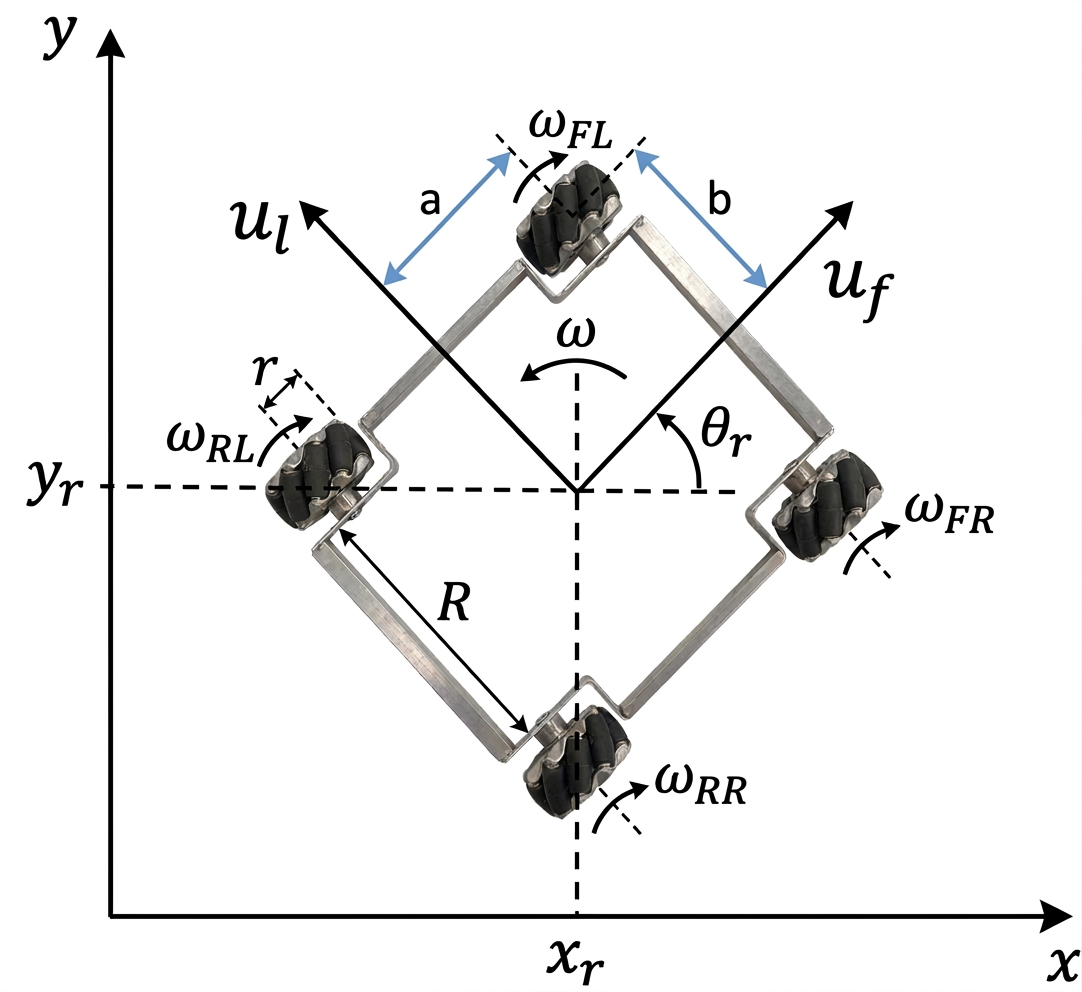
\includegraphics[width=0.5\textwidth]{images/Ch2/Kinematic model mecanum wheels.jpg}
    \caption{Kinematic parameters of a 4-wheel Mecanum drive robot. The distances $a$ and $b$ represent the longitudinal and lateral offsets of the wheels relative to the geometric center (Image adapted from Reque et al. \cite{reque_mechatronics_2021}).}
    \label{fig:mecanum_model}
\end{figure}

\subsection{Direct and Inverse Kinematics}
\label{subsec:holon direct and invecers kin}

Following the kinematic derivations proposed by Taheri et al. \cite{taheri_kinematic_2015}, the mobility of the robot is analyzed by linking the local velocities of the chassis --- namely the linear velocities $v_x$ (forward), $v_y$ (lateral) and the angular velocity $\omega$ --- to the rotational speeds of the four wheels.

The \emph{Inverse Kinematics} determines the required wheel velocities given a desired robot velocity vector $[v_x, v_y, \omega]^T$ generated by the ROS 2 navigation stack. By projecting the velocity of the robot onto the driving direction of each wheel and accounting for the $45^\circ$ slip angle of the rollers, the inverse kinematics is expressed in matrix form as \cite{taheri_kinematic_2015}:
\begin{equation}
    \begin{bmatrix}
        \omega_{FL} \\ \omega_{FR} \\ \omega_{RL} \\ \omega_{RR}
    \end{bmatrix}
    = \frac{1}{r}
    \begin{bmatrix}
         1 & -1 & -(a + b) \\
         1 &  1 &  (a + b) \\
         1 &  1 & -(a + b) \\
         1 & -1 &  (a + b)
    \end{bmatrix}
    \begin{bmatrix}
        v_x \\ v_y \\ \omega
    \end{bmatrix}
\end{equation}

Conversely, the \emph{Direct Kinematics} (or Forward Kinematics) computes the resulting robot velocity given the angular speeds of the four wheels, which is essential for odometry computation. Using the pseudo-inverse of the kinematic matrix \cite{taheri_kinematic_2015}:
\begin{equation}
    \begin{bmatrix}
        v_x \\ v_y \\ \omega
    \end{bmatrix}
    = \frac{r}{4}
    \begin{bmatrix}
         1 &  1 &  1 &  1 \\
        -1 &  1 &  1 & -1 \\
        -\frac{1}{a+b} & \frac{1}{a+b} & -\frac{1}{a+b} & \frac{1}{a+b}
    \end{bmatrix}
    \begin{bmatrix}
        \omega_{FL} \\ \omega_{FR} \\ \omega_{RL} \\ \omega_{RR}
    \end{bmatrix}
\end{equation}

\subsection{Holonomic Mobility and Constraints}
\label{subsec:holonomic_mobility}
As demonstrated by the direct kinematics matrix, the velocity vector $[v_x, v_y, \omega]^T$ can assume any arbitrary value. This mathematically proves that all 3 spatial degrees of freedom can be actuated independently and simultaneously.

To maintain formal symmetry with the differential drive analysis, the mobility of the OmniBase must be evaluated using the same Pfaffian constraint approach. For the PMB2 base, the inability to move laterally resulted in a constraint matrix $A(q)$ of rank 1. Conversely, the OmniBase imposes no differential constraints that cannot be integrated. Consequently, applying the formal approach introduced in Section 2.2.3, the associated Pfaffian constraint equation $A(q)\dot{q} = 0$ is characterized by a null constraint matrix $A(q)$:
\begin{equation}
    \begin{bmatrix} 0 & 0 & 0 \end{bmatrix} 
    \begin{bmatrix} \dot{x} \\ \dot{y} \\ \dot{\theta} \end{bmatrix} = 0
\end{equation}

Because the rank of the constraint matrix is strictly zero, the robot's degree of mobility ($\delta_M$) is exactly equal to the dimension of its planar configuration space ($\delta_M = 3$). The platform is fully holonomic. 

The ability to command a non-zero lateral velocity ($v_y \neq 0$), commonly known as \emph{strafing}, fundamentally alters how path planning algorithms compute trajectories. As noted by PAL Robotics \cite{pal_blog_omni_diff}, this holonomic capability eliminates the need for prior in-place rotations. It allows for smooth, continuous, obstacle-avoiding maneuvers in extremely confined spaces, enabling the robot to maintain a fixed sensory viewpoint (e.g., keeping a camera pointed at a target) while translating seamlessly around it.




\section{Probabilistic Motion Models}
\label{sec:probabilistic_motion_models}

The kinematic formulations derived in the preceding sections provide a deterministic framework for mapping control inputs to the ideal velocities of both the differential and holonomic mobile bases. However, executing navigation tasks in physical or high-fidelity simulated environments introduces a profound divergence between ideal kinematic predictions and actual robot trajectories. To bridge this gap, the deterministic perspective must be replaced by a probabilistic approach that explicitly models the inherent stochasticity of physical interactions. This section establishes the theoretical foundations of probabilistic motion models, transitioning from general actuation uncertainty to the specific odometric noise profiles that characterize the PMB2 and OmniBase platforms.

\subsection{Introduction to Odometry-Based Motion Models}
\label{subsec:intro_odometry_models}
The kinematic models previously analyzed rely on the ideal assumption of pure rolling and no slipping. In real-world applications, however, a mobile robot can never be tracked perfectly through the simple integration of its kinematic equations over time—a practice traditionally known as dead reckoning. The execution of a control command at any given time step $t$ is invariably affected by structural, mechanical, and environmental disturbances, such as wheel slippage, limited encoder resolution, and floor irregularities. 

To robustly navigate under these uncontrollable factors, modern robotics shifts from deterministic kinematics to a probabilistic approach, formalized by Thrun et al. \cite{thrun_probabilistic_2005}. Within this framework, the motion of the robot is modeled as a conditional probability density function (PDF), known as the \emph{motion model}:
\begin{equation}
    p(q_t \mid u_t, q_{t-1}),
\end{equation}
where $q_t$ and $q_{t-1}$ represent the current and previous global poses of the robot in its configuration space, respectively, and $u_t$ denotes the motion input.

In practical autonomous navigation frameworks like ROS 2, the motion input $u_t$ utilized by state estimation and localization algorithms (such as the Adaptive Monte Carlo Localization, or AMCL) is typically not the commanded velocity vector, but rather the \emph{odometry reading} obtained from the wheel encoders. As noted by Thrun et al. \cite{thrun_probabilistic_2005}, odometry-based motion models are generally superior to velocity-based models because encoders directly measure the actual wheel revolutions. This allows the system to inherently capture some of the mechanical discrepancies and actual displacements that a pure software velocity command would completely miss.

The underlying sources of this odometric uncertainty can be classified into systematic and non-systematic errors \cite{thrun_probabilistic_2005}. Systematic errors stem from physical imperfections of the platform, such as unequal wheel diameters or structural misalignments, which introduce a deterministic drift that accumulates predictably. Non-systematic errors, conversely, are entirely stochastic and originate from unpredictable dynamic interactions, including wheel slippage on low-friction surfaces or structural vibrations. 

While odometry provides highly accurate relative displacement data over short intervals, the continuous integration of both systematic and non-systematic errors inevitably leads to unbounded \emph{dead-reckoning drift}. The critical aspect of this work is that the mathematical structure and spatial propagation of this probabilistic noise are strictly dictated by the robot's kinematics. This structural divergence establishes a fundamentally different error accumulation profile between the differential PMB2 and the holonomic OmniBase.

\subsection{Differential Drive Uncertainty (PMB2)}
\label{subsec:differential_uncertainty}
The estimation of odometric uncertainty for the non-holonomic TIAGo PMB2 base is modeled by decomposing the relative movement between two consecutive global poses, $q_{t-1}$ and $q_t$, into three sequential stochastically independent maneuvers (Figure~\ref{fig:thrun_decomposition}): an initial rotation ($\delta_{\text{rot1}}$), a translation ($\delta_{\text{trans}}$), and a final corrective rotation ($\delta_{\text{rot2}}$) \cite{thrun_probabilistic_2005}.

In real-world operations, the actual execution of these components diverges from the nominal encoder readings due to mechanical and environmental disturbances. Following the probabilistic framework established by Thrun et al. \cite{thrun_probabilistic_2005}, the variances ($\sigma^2$) of these error distributions are structurally coupled to the magnitude of the commanded motion parameters through four platform-specific noise coefficients, $\alpha_1, \alpha_2, \alpha_3,$ and $\alpha_4$:
\begin{align}
    \sigma^2_{\text{rot1}} &= \alpha_1 \delta^2_{\text{rot1}} + \alpha_2 \delta^2_{\text{trans}}, \\
    \sigma^2_{\text{trans}} &= \alpha_3 \delta^2_{\text{trans}} + \alpha_4 \left( \delta^2_{\text{rot1}} + \delta^2_{\text{rot2}} \right), \\
    \sigma^2_{\text{rot2}} &= \alpha_1 \delta^2_{\text{rot2}} + \alpha_2 \delta^2_{\text{trans}}.
\end{align}

\begin{figure}[htbp]
    \centering
    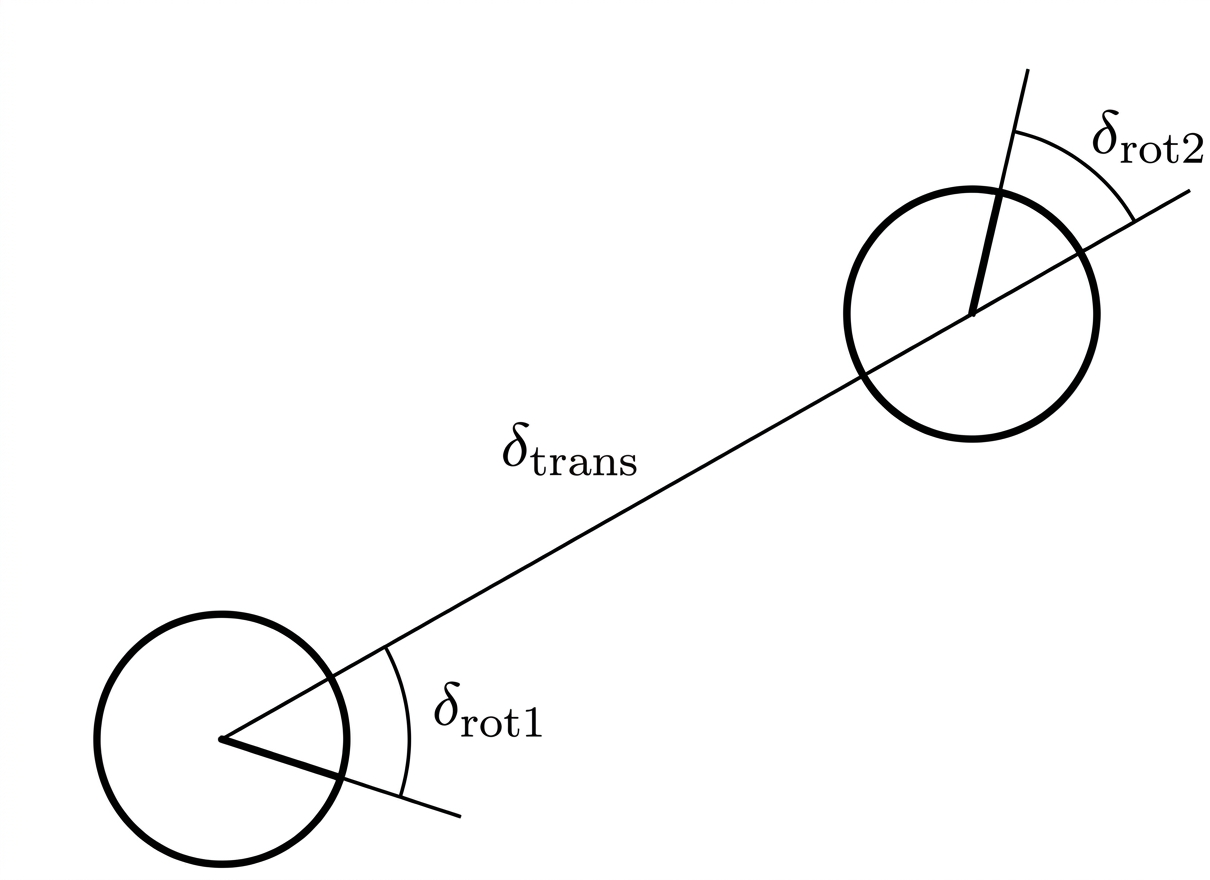
\includegraphics[width=0.5\textwidth]{images/Ch2/Spostamento in tre fasi.jpg}
    \caption{Decomposition of the relative movement between two consecutive poses into an initial rotation, a straight-line translation, and a final corrective rotation (Image adapted from \cite{thrun_probabilistic_2005}).}
    \label{fig:thrun_decomposition}
\end{figure}

For the PMB2 platform, the non-holonomic constraint formulated in Equation~(2.5) dictates that the local lateral velocity must strictly satisfy $v_y = 0$. Consequently, no instantaneous lateral drift can be directly generated within the robot's local frame. Instead, the characteristic "banana-shaped" uncertainty profile (Figure~\ref{fig:banana_shape}) arises because early orientation errors ($\sigma^2_{\text{rot1}}$), caused by wheel micro-slippage or encoder resolution limits during rotation, are geometrically amplified by the subsequent longitudinal translation $\delta_{\text{trans}}$ \cite{thrun_probabilistic_2005}.

\begin{figure}[htbp]
    \centering
    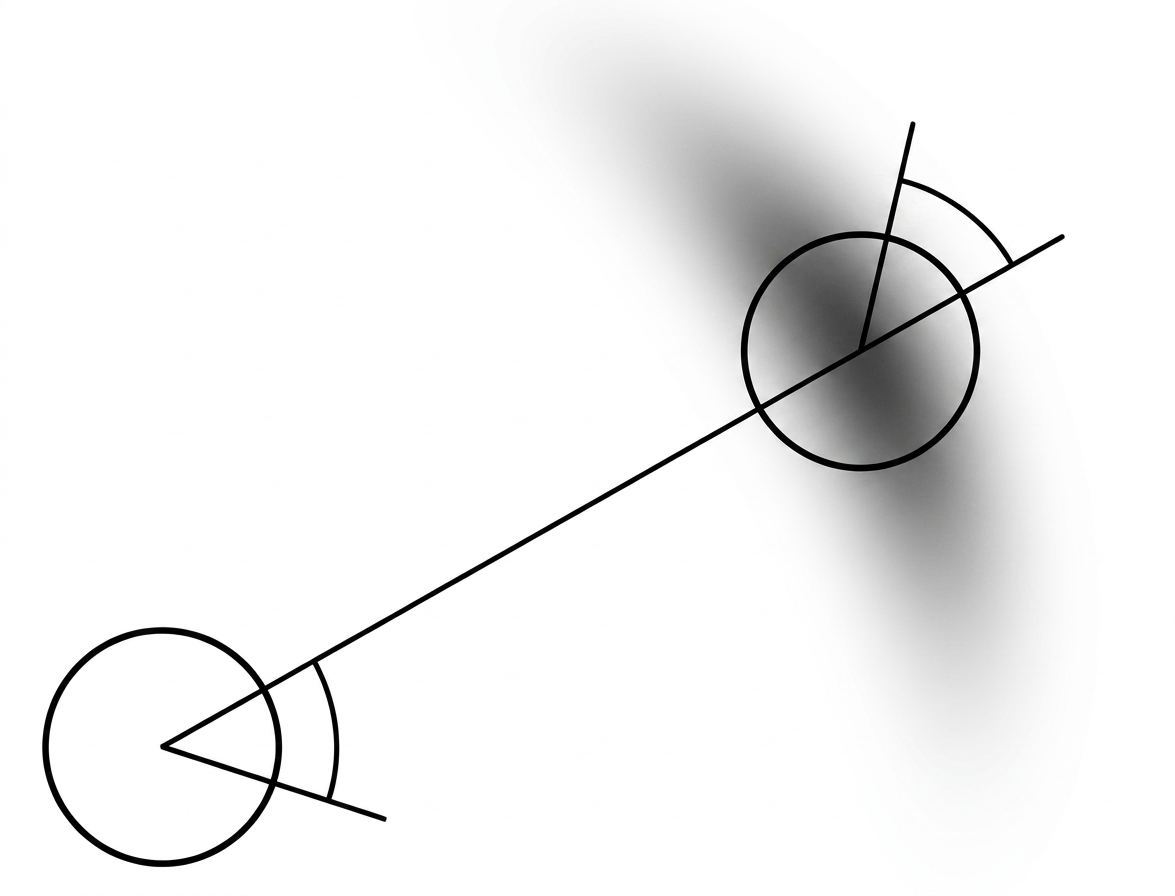
\includegraphics[width=0.5\textwidth]{images/Ch2/Banana shape distribution.jpg}
    \caption{Characteristic "banana-shaped" probability distribution of a differential drive robot. The geometric profile results from early rotational uncertainties being amplified by the subsequent forward translation (Image adapted from \cite{thrun_probabilistic_2005}).}
    \label{fig:banana_shape}
\end{figure}

This makes the bounding of angular variance a critical requirement for the localization stack during forward navigation.


\subsection{Holonomic Drive Uncertainty (OmniBase)}
\label{subsec:holonomic_uncertainty}
In stark contrast to the differential drive, the TIAGo OmniBase utilizes four Mecanum wheels to achieve full holonomic mobility. The fundamental mechanical principle of these wheels relies on passive rollers mounted at a $45^{\circ}$ angle (Figure~\ref{fig:mecanum_forces}). While this design enables instantaneous translations in any planar direction, it purposefully induces continuous, controlled slippage during navigation. 

\begin{figure}[H]
    \centering
    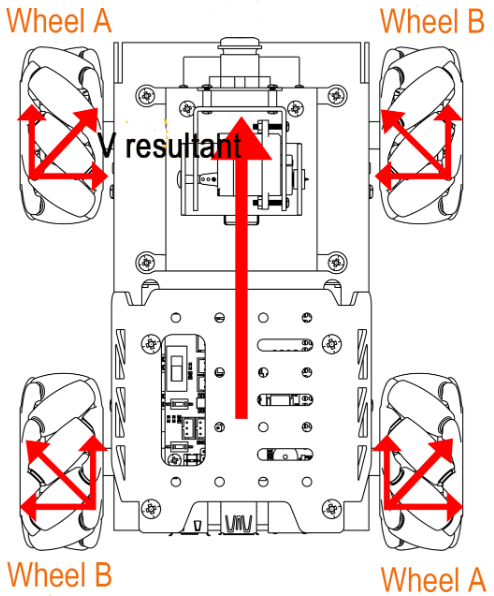
\includegraphics[width=0.40\textwidth]{images/Ch2/Forze risultanti mecanum.png}
    \caption{Kinematic force vectors acting on a Mecanum wheel, illustrating the $45^{\circ}$ orientation of the passive rollers responsible for controlled, multi-directional slippage (Image adapted from \cite{hiwonder_mecanum_2026}).}
    \label{fig:mecanum_forces}
\end{figure}

From a probabilistic perspective, as discussed by Thrun et al. \cite{thrun_probabilistic_2005}, this physical characteristic significantly alters the odometric noise distribution. Unlike the PMB2, the OmniBase is not subject to the non-holonomic lateral constraint ($v_y = 0$). Therefore, the standard unicycle decomposition ($\delta_{\text{rot1}}, \delta_{\text{trans}}, \delta_{\text{rot2}}$) is geometrically inadequate. For a holonomic platform, the relative odometric displacement between two consecutive poses, $q_{t-1}$ and $q_t$, is directly extracted in the robot's local frame as a generic translation along the longitudinal axis ($\delta_x$), a translation along the lateral axis ($\delta_y$), and a rotation ($\delta_\theta$).

Because lateral displacements are both intentionally commanded and inherently affected by the stochastic slippage of the passive rollers, the error propagates simultaneously and is highly coupled across all Cartesian axes. Analogously to the differential model, the variances ($\sigma^2$) for the holonomic drive can be explicitly formulated by mapping the commanded local displacements to the error distributions via a new set of specific noise coefficients, $\alpha_1$ through $\alpha_9$:
\begin{align}
    \sigma^2_{x} &= \alpha_1 \delta_x^2 + \alpha_2 \delta_y^2 + \alpha_3 \delta_\theta^2, \\
    \sigma^2_{y} &= \alpha_4 \delta_x^2 + \alpha_5 \delta_y^2 + \alpha_6 \delta_\theta^2, \\
    \sigma^2_{\theta} &= \alpha_7 \delta_x^2 + \alpha_8 \delta_y^2 + \alpha_9 \delta_\theta^2.
\end{align}

\begin{figure}[H]
    \centering
    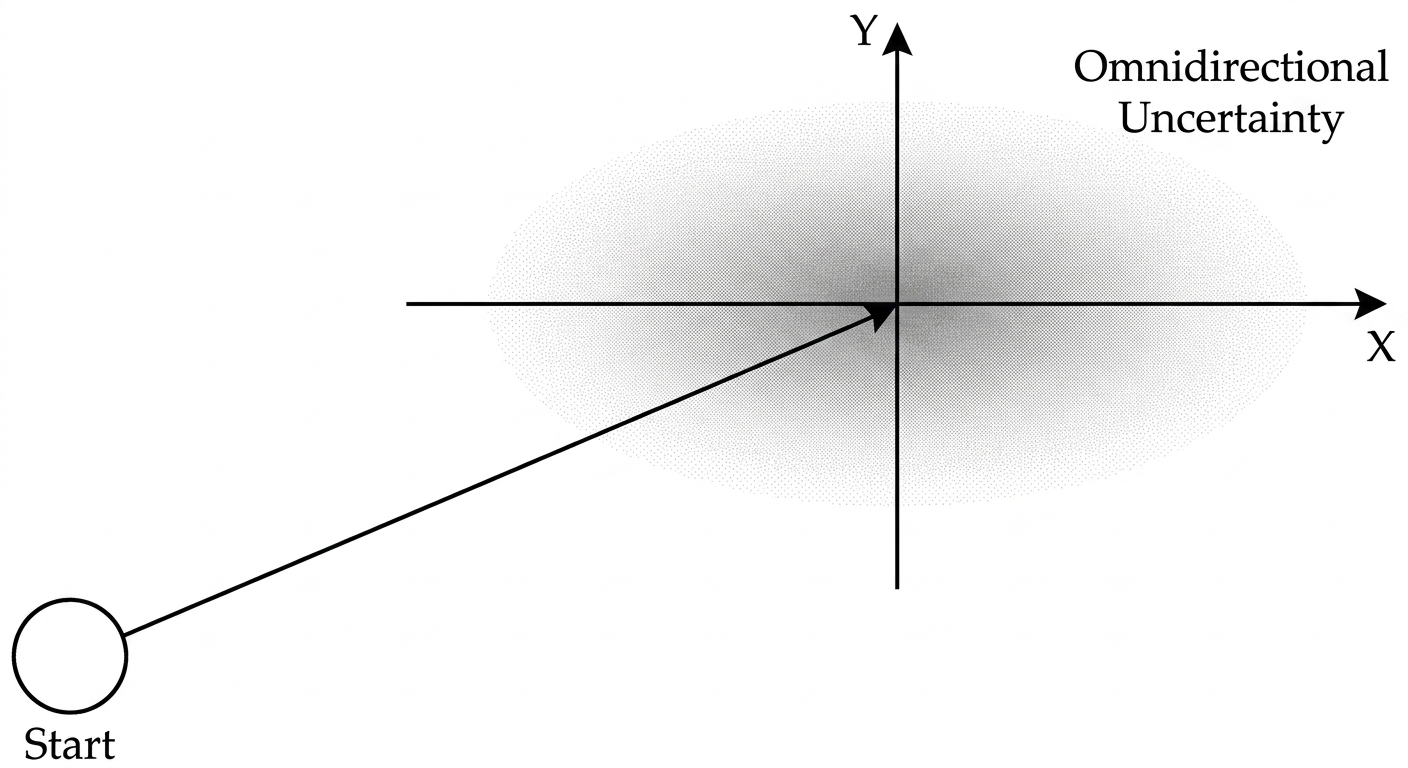
\includegraphics[width=0.7\textwidth]{images/Ch2/cloud shape distribution.jpg}
    \caption{Characteristic probability cloud of an omnidirectional drive. The unconstrained lateral slippage generates a broad uncertainty distribution across all axes, contrasting with the differential "banana-shape".}
    \label{fig:cloud_shape}
\end{figure}

This mathematical formulation clearly demonstrates that the lateral variance $\sigma^2_{y}$ is no longer bounded or negligible. The cross-coupling terms (for example, the influence of the lateral motion $\delta_y$ on the rotational error $\sigma^2_\theta$) dictate that the resulting uncertainty profile expands into a broader, omnidirectional probability cloud (Figure~\ref{fig:cloud_shape}), rather than a tightly constrained curve. This structural variance necessitates more frequent and robust sensory updates from the Nav2 localization stack to prevent rapid dead-reckoning drift during complex holonomic maneuvers.

In practice, the ROS~2 Nav2 framework does not implement this full
nine-coefficient covariance: its \texttt{nav2\_amcl::OmniMotionModel} adopts
a reduced five-parameter form, whose rationale and parameterisation are
detailed in Section \ref{subsec:amcl_tuning}.


\subsection{Comparative Odometry Noise Profile}
\label{subsec:comparative_noise_profile}
The structural and kinematic divergence between the differential PMB2 and the holonomic OmniBase establishes a fundamental trade-off between vehicular mobility and odometric reliability. A systematic comparison of their probabilistic motion models reveals distinct error propagation behaviors that directly influence state estimation.

The non-holonomic PMB2 base features a tightly constrained noise profile. Because it satisfies the zero lateral velocity constraint ($v_y = 0$), the instantaneous generation of lateral drift within the local frame is physically restricted. The odometric uncertainty is primarily driven by rotational noise, which geometrically expands into the characteristic banana-shaped distribution along the transverse axis during forward translation \cite{thrun_probabilistic_2005}. This localized error accumulation allows localization algorithms, such as AMCL within the Nav2 stack, to predict and bound the position variance effectively using highly directional sensory updates.

Conversely, the holonomic OmniBase exhibits a continuous, omnidirectional error propagation. The absence of the lateral velocity constraint enables full planar maneuverability but introduces a highly coupled noise distribution across the $X$, $Y$, and $\theta$ axes simultaneously. This is a direct consequence of the continuous, unmodeled slippage generated by the $45^{\circ}$ passive rollers inherent to the Mecanum wheel design. The resulting uncertainty expands as a broad omnidirectional probability cloud rather than a constrained curve, necessitating more frequent sensor fusion updates to counteract rapid dead-reckoning drift. Consequently, tuning the probabilistic motion parameters within ROS~2 requires the introduction of an additional noise coefficient (the lateral term $\alpha_5$), absent in the differential model, to bound the extra lateral slippage variance and prevent filter divergence during complex, multidirectional maneuvers; the four differential coefficients $\alpha_1$--$\alpha_4$ are themselves kept identical across both platforms.


%!TeX root = ../main.tex

% ==========================================
% CHAPTER 3: SYSTEM ARCHITECTURE AND ROS 2 SETUP
% ==========================================
\chapter{System Architecture and Infrastructure Development}
\label{ch:architecture}

This chapter details the software architecture, the simulation environment setup, and the extensive infrastructural modifications required to execute a fair and rigorous comparative analysis. The default packages provided by the manufacturer were fundamentally tailored for differential drive operations. Consequently, a significant systems engineering effort was necessary to decouple the hardcoded dependencies, resolve simulation rendering and physics engine artifacts, and fine-tune the navigation algorithms for holonomic mobility.

\section{The ROS 2 Framework and Nav2 Stack}

The software architecture of this thesis is built upon the Robot Operating System 2 (ROS 2), specifically the \textit{Humble Hawksbill} distribution. Within this framework, autonomous navigation is governed by the Navigation 2 (Nav2) stack. Nav2 is a highly modular, behavior-tree-based navigation system, conceptually divided into several distinct servers. To establish a rigorous baseline for the comparative analysis, the following specific algorithmic configurations were selected:

\begin{itemize}
    \item \textbf{Planner Server:} Computes the optimal global path from the robot's current position to a goal pose using the global costmap. For this work, the \texttt{NavfnPlanner} was employed. In the waypoint-navigation experiments it was run in Dijkstra mode (\texttt{use\_astar: false}), which performs a full wavefront expansion and returns the minimum-cost geometric path. For the autonomous-exploration experiments, where the planner is repeatedly queried for distant frontier goals, the A* heuristic was instead enabled (\texttt{use\_astar: true}) to reduce the expansion cost of each planning query.
    \item \textbf{Controller Server:} Acts as the local planner, computing the immediate velocity commands ($\vec{v} = [v_x, v_y, \omega]^T$) required to follow the global path while dynamically avoiding local obstacles. The \texttt{DWBLocalPlanner} was selected for this core task.
    \item \textbf{Behavior Server:} Manages recovery behaviors (such as clearing costmaps, backing up, or spinning in place) when the robot detects a failure or gets stuck in complex environments.
    \item \textbf{AMCL (Adaptive Monte Carlo Localization):} A probabilistic localization system that utilizes a particle filter to track the robot's pose against a known map, comparing the expected environmental geometry with real-time LiDAR scans.
\end{itemize}

The localization component depends on the experimental campaign. In the \\ waypoint-navigation experiments the map of the environment is known in advance, and the robot pose is tracked by AMCL as described above. In the autonomous-exploration experiments, by contrast, no prior map is available: localization and mapping are performed simultaneously by \texttt{slam\_toolbox} running in \texttt{mapping} mode, which incrementally builds the occupancy grid from LiDAR scan matching (using a Ceres-based pose-graph back-end) and feeds it to the Nav2 costmaps. The two campaigns therefore rely on two distinct localization regimes---AMCL on a known map for waypoint navigation, and online simultaneous localisation and mapping (SLAM) for exploration---a distinction that must be kept in mind when comparing the pose-related metrics of the two tasks.

The choice of the \texttt{DWBLocalPlanner} as the local controller is particularly significant for this study. Because its architectural legacy is a direct evolution of the Dynamic Window Approach (DWA), it inherently embodies the differential-drive bias prevalent in current industry standards. Employing it as the baseline provides a concrete starting point to evaluate the behavior of holonomic kinematics under legacy constraints, mathematically highlighting the necessity of holonomic-specific tuning.

\section{The TIAGo Robotic Platform}

The experimental evaluations are conducted using the TIAGo robot, developed by PAL Robotics. TIAGo is a highly modular service robot featuring a 7-DOF manipulator arm, a lifting torso, and an array of perception sensors mounted on its head. The critical feature of this platform, which makes it ideal for this comparative study, is its interchangeable mobile base. The upper body remains identical, ensuring that payload, sensor placement, and center of mass distributions are largely consistent, thereby isolating the kinematic drive as the primary variable.

\subsection{Differential Drive Configuration (PMB2)}
The default configuration employs the PAL Mobile Base 2 (PMB2, Figure~\ref{fig:PMB2 base}) \cite{pal_tiago_base}. This non-holonomic base is characterized by a two-wheel differential drive mechanism supported by caster wheels. 
From a software and collision-avoidance perspective, the PMB2 is modeled with a strictly circular static footprint with a radius of $0.275$ meters. Environmental perception for obstacle avoidance and AMCL localization is achieved via a single forward-facing 2D LiDAR, whose data is broadcasted on the standard \texttt{/scan\_raw} topic.

\begin{figure}[H]
    \centering
    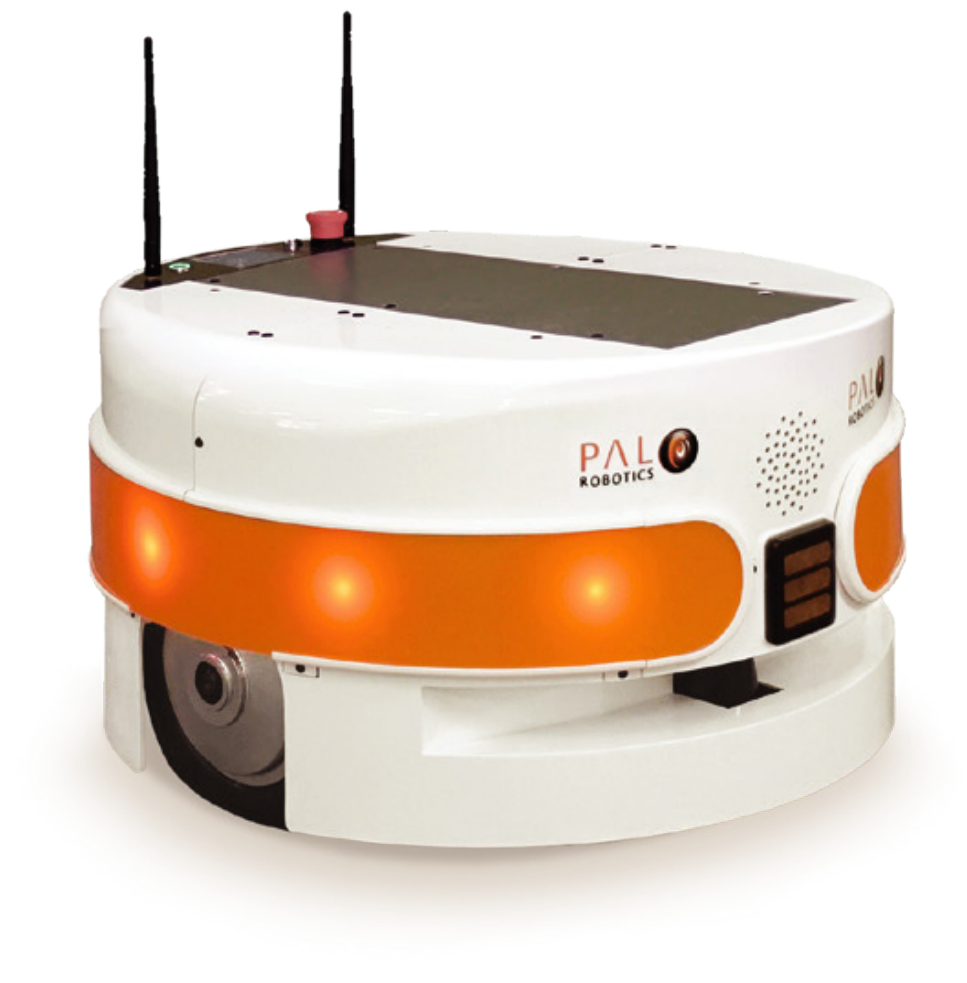
\includegraphics[width=0.4\textwidth]{images/Ch3/pmb2.png}
    \caption{PAL Robotics - PMB2 base}
    \label{fig:PMB2 base}
\end{figure}

\subsection{Omnidirectional Configuration (OmniBase)}
The alternative configuration substitutes the PMB2 with the OmniBase (Figure~\ref{fig:Omni base}) \cite{pal_tiago_omnibase}, a holonomic platform equipped with four independently driven Mecanum wheels. 
This configuration diverges significantly from the PMB2 in its physical footprint and sensory layout (Figure~\ref{fig:tiago_bases}). Due to the geometric constraints of mounting four Mecanum wheels parallel to the longitudinal axis, the OmniBase requires a rectangular footprint (defined in the local frame by the vertices \\ $[0.35, 0.24], [-0.35, 0.24], [-0.35, -0.24], [0.35, -0.24]$ in meters). Furthermore, to ensure complete 360-degree visibility without blind spots caused by the rectangular chassis, the OmniBase is equipped with two 2D LiDAR sensors, mounted diagonally (front-left and rear-right). Consequently, the sensory data is published on two distinct topics: \texttt{/scan\_front\_raw} and \texttt{/scan\_rear\_raw}.

These seemingly minor hardware differences have profound implications on the configuration of the Nav2 stack, particularly concerning footprint generation in the local and global costmaps and the correct ingestion of sensory data by the AMCL localization module.

\begin{figure}[H]
    \centering
    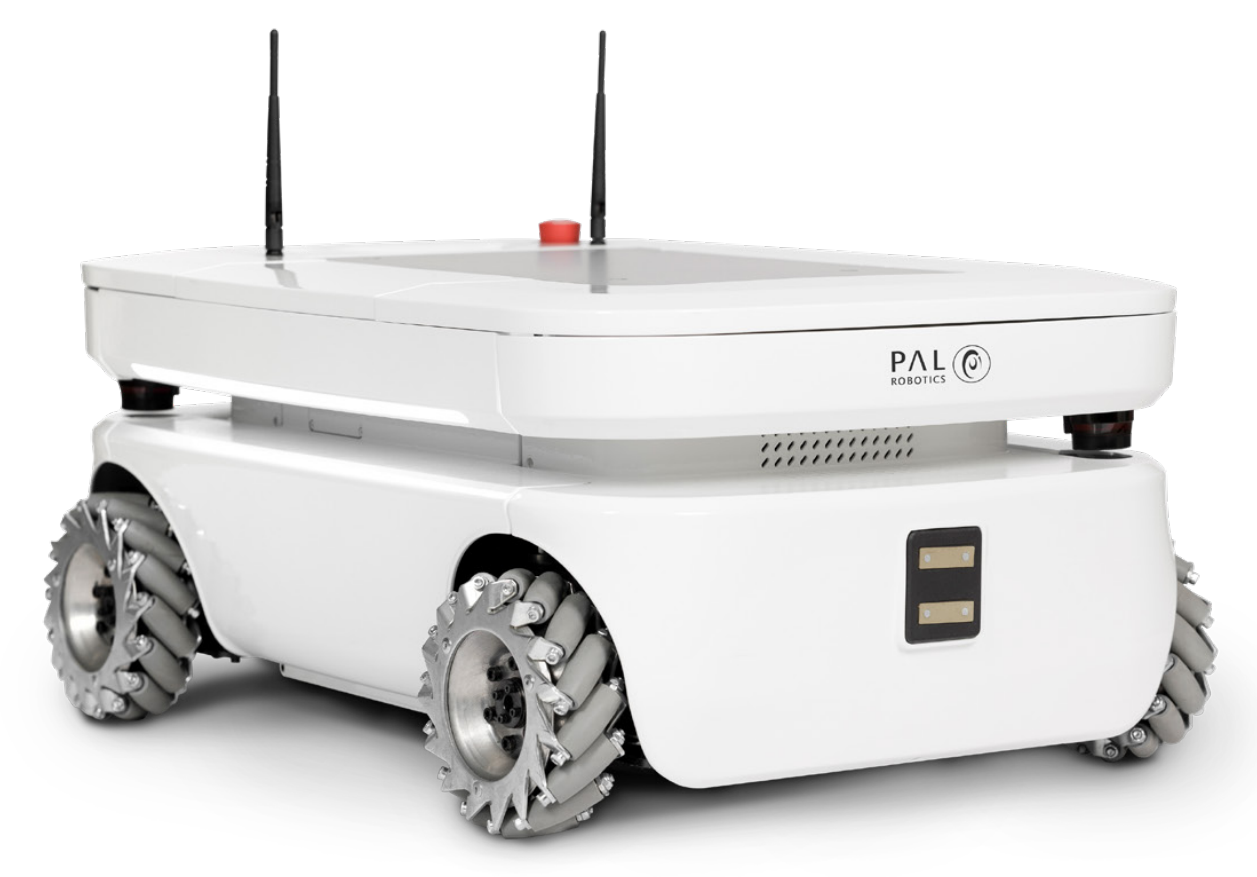
\includegraphics[width=0.4\textwidth]{images/Ch3/omni.png}
    \caption{PAL Robotics - OmniBase}
    \label{fig:Omni base}
\end{figure}

\begin{figure}[H]
     \centering
     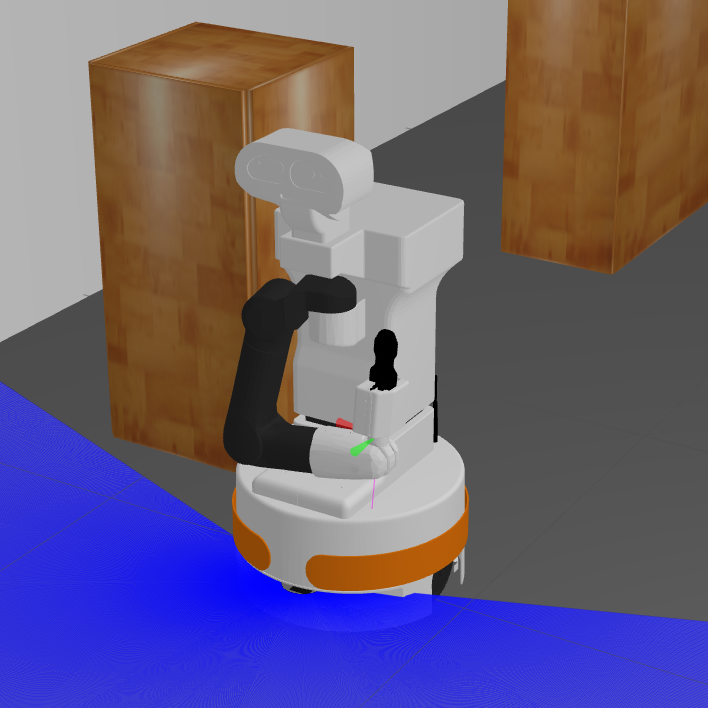
\includegraphics[width=0.45\textwidth]{images/Ch3/pmb2_gazebo.png}
     \hfill
     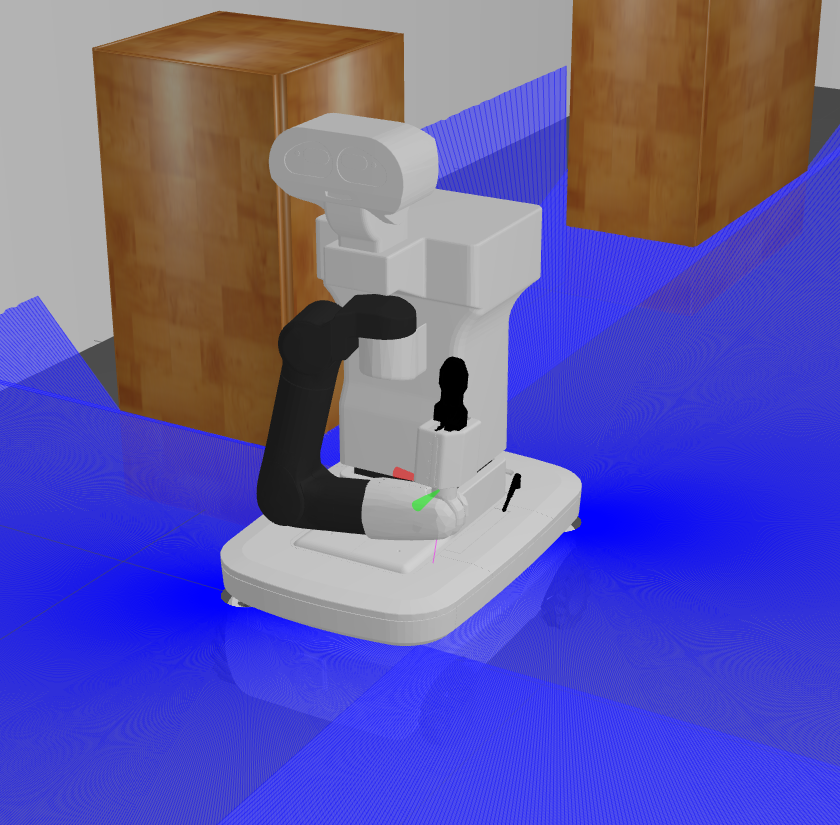
\includegraphics[width=0.45\textwidth]{images/Ch3/omni_gazebo.png}
     \caption{Comparison of the TIAGo mobile bases in Gazebo. Left: The PMB2 differential drive base. Right: The OmniBase with Mecanum wheels.}
     \label{fig:tiago_bases}
\end{figure}

\subsection{Simulation Hardware Specifications}
Because the comparative analysis heavily relies on the physical execution time and the Real-Time Factor (RTF) of the simulation, the hardware specifications of the deployment workstation must be explicitly stated to ensure scientific reproducibility. 

All experiments and simulations were executed natively on Ubuntu 22.04 LTS. The workstation is powered by an AMD Ryzen 5 3600 6-Core Processor, equipped with 32 GB of RAM, and utilizes an AMD Radeon RX 5600 XT Graphics Processing Unit. Documenting this specific GPU architecture is particularly relevant, as its direct interaction with the Gazebo OpenGL rendering pipeline motivated the environmental workarounds implemented in the subsequent section to stabilize the simulation frame rate.

\section{Workspace Setup and Simulation Fixes}
\label{sec:ws setup}

Setting up a robust simulation environment required resolving several low-level dependencies and hardware-specific bottlenecks that initially prevented the execution of the experiments.

\subsection{Dependencies and URDF Conflicts}
The provided ROS 2 workspace was initially configured exclusively for the PMB2 differential base. To enable the omnidirectional configuration, the official \texttt{omni\_base} packages were integrated into the workspace. Furthermore, the pre-installed \texttt{pal\_urdf\_utils} package originated from an unofficial repository, resulting in missing files during compilation. This was resolved by replacing it entirely with the official upstream branch.

A critical simulation failure occurred during the spawning of the TIAGo model, where the Gazebo server crashed with a segmentation fault upon initialization. Debugging revealed a namespace collision: both the standard TIAGo description and the OmniBase description attempted to instantiate an IMU plugin named \texttt{base\_imu}. To resolve this conflict, the plugin was renamed to \texttt{tiago\_base\_imu} directly within the Xacro definitions (the stream editor command used for this programmatic refactoring is provided in Appendix \ref{app:urdf_conflict}).

\subsection{GPU Rendering Optimization}
\label{subsec:gpu optimization}
During the initial testing phase on the AMD-equipped workstation, a hardware-rendering issue was identified: the physics engine failed to compute and visualize the LiDAR sensors of the OmniBase. Forcing the system to utilize CPU-based software rendering (via the \\ \texttt{LIBGL\_ALWAYS\_SOFTWARE=1} environment variable) successfully resolved the sensor computation issue. However, applying this globally caused the simulation performance to plummet to an unusable 9 Frames Per Second (FPS).

To bypass this bottleneck, a targeted bash wrapper was implemented. Instead of forcing software rendering on the entire simulation—including the graphical client (\texttt{gzclient})—the wrapper applies the variable exclusively to the Gazebo physics server (\texttt{gzserver}). The bash implementation of this targeted wrapper is documented in Appendix \ref{app:gzserver_wrapper}. This decoupling restored the simulation's viability, keeping the Real-Time Factor (RTF) in a consistent range---around $0.9$ under sustained navigation load, with short, lightly loaded runs occasionally reaching or exceeding $1.0$ (an artefact of averaging the factor over a very small time window). Because the RTF is generally at or slightly below $1.0$, the simulation clock runs at, or slightly slower than, the system wall time. It therefore became an absolute necessity to enforce and propagate the \texttt{use\_sim\_time:=true} parameter across the entire ROS~2 testing pipeline. This ensured that all nodes, controllers, and data loggers synchronised perfectly with Gazebo's internal \texttt{/clock} topic, preserving temporal consistency and guaranteeing that the comparative performance metrics remained scientifically valid regardless of the hardware-induced slowdown.

\subsection{Simulation Environments and Ground Truth Extraction}
\label{subsec:simulation_gt}
To thoroughly evaluate the platforms, two distinct Gazebo environments were utilized. For the directed waypoint navigation tests, the stock PAL Robotics \texttt{small\_office} world was used as a baseline. This environment required minor modifications to suit the benchmarking needs: the lighting was adjusted, specific obstacles like overhanging tall desks (which caused blind collisions) were removed, and static human models were added to simulate a realistic, cluttered office scenario. 
Conversely, for the autonomous exploration benchmarks, the \texttt{home} world was deployed. This environment represents a realistic domestic apartment and was left entirely unaltered to provide a highly complex scenario.

Crucially, to enable rigorous scientific evaluation, the system was configured to log the absolute Ground Truth pose of the robot across both environments. As theoretically established in Section \ref{sec:probabilistic_motion_models}, relying solely on raw odometry for error calculation would introduce an inherent estimation bias due to unbounded dead-reckoning drift. Furthermore, while localization algorithms like AMCL act to bound this drift, they inherently introduce stochastic estimation noise due to particle variance. Because the PMB2 and OmniBase generate fundamentally different probabilistic noise profiles (constrained vs. omnidirectional distributions), evaluating their path-tracking performance via their own onboard estimation would invalidate the fairness of the comparison. To ensure that the offline trajectory analyses remained strictly objective and uncontaminated by these uncertainties, the \texttt{gazebo\_ros\_state} plugin was injected into both \texttt{.world} configurations (the XML implementation of this plugin is available in Appendix \ref{app:gt_plugin}). This plugin publishes the absolute spatial coordinates of all simulated models to the ROS 2 network at a frequency of 50 Hz, providing an infallible spatial reference.

\section{The Master Launch Architecture and Dynamic Initialization}
\label{sec:launch arch}

The default launch infrastructure provided by the manufacturer lacked native support for arbitrary spawn coordinates, dynamic simulation environments, and base swapping. To systematically benchmark the two kinematic models, a custom master launch  \\ (\texttt{tiago\_thesis\_gazebo.launch.py}) was developed to orchestrate a controlled and repeatable initialization sequence, effectively acting as an initialization state-machine.

\subsection{Propagating the Kinematic Profile}
In the ROS 2 launch system, configurations are structured as an inverted tree. To allow the runtime dynamic selection of the robot's kinematics, the \texttt{base\_type} parameter was explicitly routed through the intermediate launch files down to the state publisher and controller multiplexer. The main robot description file was then refactored using conditional logic. This ensures that Gazebo dynamically assembles the correct 3D meshes, hardware controllers, and LiDAR layouts based purely on the propagated argument.

\subsection{The Odometry TF Bridge}
\label{subsec:odom tf bridge}
A critical simulation anomaly emerged exclusively when testing the OmniBase. In simulation, the holonomic base is driven by the \texttt{gazebo\_ros\_planar\_move} plugin to bypass the prohibitive computational cost of simulating physical friction on the Mecanum rollers. However, this plugin inherently bypasses the standard \texttt{ros2\_control} architecture and joint states mechanisms, failing to broadcast the essential Transform (TF) from the \texttt{odom} frame to the \texttt{base\_footprint} frame.

Because Nav2 requires a continuous TF tree, the absence of this transform causes the stack to crash upon initialization. To bridge this gap, a custom Python node (\texttt{odom\_tf\_publisher.py}) was developed to subscribe to the odometry topic and manually broadcast the missing transform (Figure~\ref{fig:tf_tree_cropped}) (the source code for this bridge is available in Appendix \ref{app:tf_bridge}). Crucially, the node was engineered to ingest the simulation time arguments, ensuring perfect temporal synchronization with the Gazebo clock. 

Beyond the missing transform, the fact that \texttt{gazebo\_ros\_planar\_move} imposes the commanded body twist directly---rather than actuating the wheels through a dynamic model, as \texttt{ros2\_control} does for the PMB2---has implications for the fairness of the kinematic comparison. These are discussed together with the evaluation metrics in Section~\ref{subsec:m-fidelity}.

\begin{figure}[H]
    \centering
    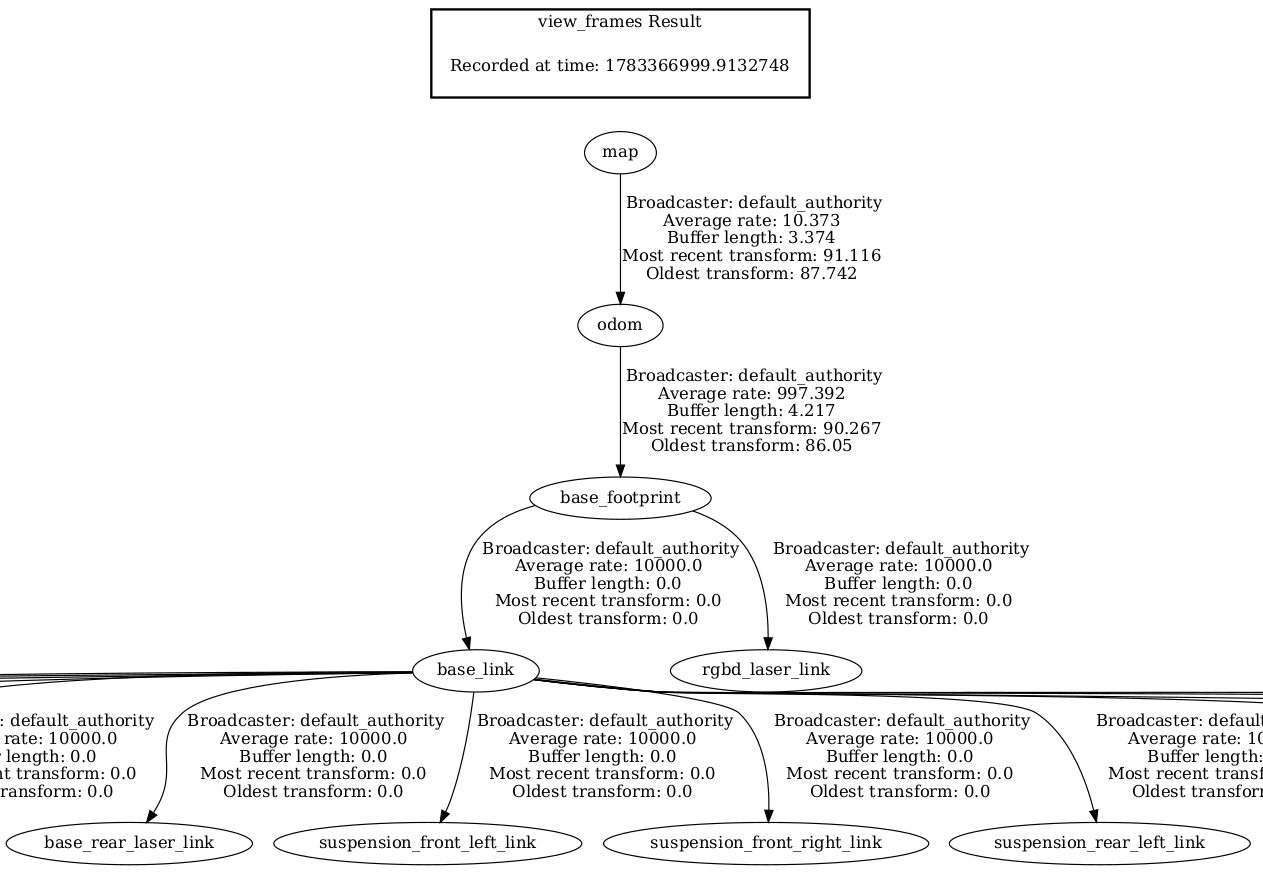
\includegraphics[width=1\textwidth]{images/Ch3/frames_diff_obs_cropped.png} 
    \caption{A heavily cropped extract of the ROS 2 TF tree for the OmniBase configuration, generated via \texttt{tf2\_tools}. The extensive kinematic branches of the upper body and auxiliary sensors have been omitted to highlight the localization root frames. Crucially, the fundamental \texttt{odom} $\rightarrow$ \texttt{base\_footprint} transform is successfully broadcasted by the custom \texttt{odom\_tf\_publisher.py} node, ensuring the continuity of the tree.}
    \label{fig:tf_tree_cropped}
\end{figure}

\subsection{Deterministic Initialization State-Machine}
\label{subsec: Deterministic Init}
To guarantee a rigorously standardized starting condition for every experimental iteration, automated routines for postural stability and spatial initialization were embedded into the launch sequence.

Spawning the TIAGo robot with its heavy 7-DOF manipulator arm fully extended creates a severe center-of-mass imbalance. Coupled with the physics engine's micro-slippage, this induces involuntary rotation upon spawning. Furthermore, since the objective of this thesis is to compare the mobile bases, an extended arm would introduce misleading spatial constraints, forcing the local planner to trigger avoidance maneuvers that do not reflect the true footprint of the base. To prevent this, the launch orchestrator actively sends a joint trajectory goal immediately at boot, transitioning the robot into a stable state by folding the arm into a compact, centralized position.

In addition to postural stability, precise spatial initialization was enforced through a dynamic teleportation routine. The orchestrator reads the user-defined coordinates and employs a robust polling loop that continually queries the ROS 2 service list (the bash implementation of this routine is detailed in Appendix \ref{app:teleport}). The teleportation payload is dispatched strictly after the physics engine fully exposes the entity manipulation service, guaranteeing that every benchmarking sequence commences from the precise mathematical coordinates required by the methodology.

\section{Navigation Stack Configuration and Algorithmic Tuning}
\label{sec:nav2_tuning}

The transition from a differential to a holonomic drive cannot be handled solely at the hardware and physics-engine levels. To conduct a fair evaluation, the Navigation 2 stack had to be profoundly reconfigured. The default parameters heavily penalize lateral movements, forcing the OmniBase into a sub-optimal "pseudo-differential" behavior. This section details the systematic parameter tuning implemented to unlock the holonomic capabilities of the OmniBase while maintaining a standardized baseline for the PMB2.

\subsection{Sensory Configuration and AMCL Probabilistic Tuning}
\label{subsec:amcl_tuning}

The physical layout of the sensors directly dictates how the robot perceives its environment and localizes itself. The differential PMB2 utilizes a single forward-facing LiDAR, whose data is broadcasted on the \texttt{/scan\_raw} topic. Conversely, to prevent blind spots along its rectangular chassis, the OmniBase relies on two LiDARs (\texttt{/scan\_front\_raw} and \texttt{/scan\_rear\_raw}). 

To ensure the \texttt{nav2\_costmap\_2d} server correctly generated the obstacle layers for the OmniBase, both the local and global costmaps were modified. The \texttt{observation\_sources} parameter was expanded to ingest both laser topics simultaneously, actively fusing the point clouds to generate a 360-degree collision map. However, because standard AMCL implementations primarily ingest a single 2D scan for particle evaluation, the localization node was explicitly routed to the primary front laser. This decoupled architectural flow is clearly visible in the active ROS 2 node graph (Figure \ref{fig:laser_graphs}).

\begin{figure}[H]
    \centering
    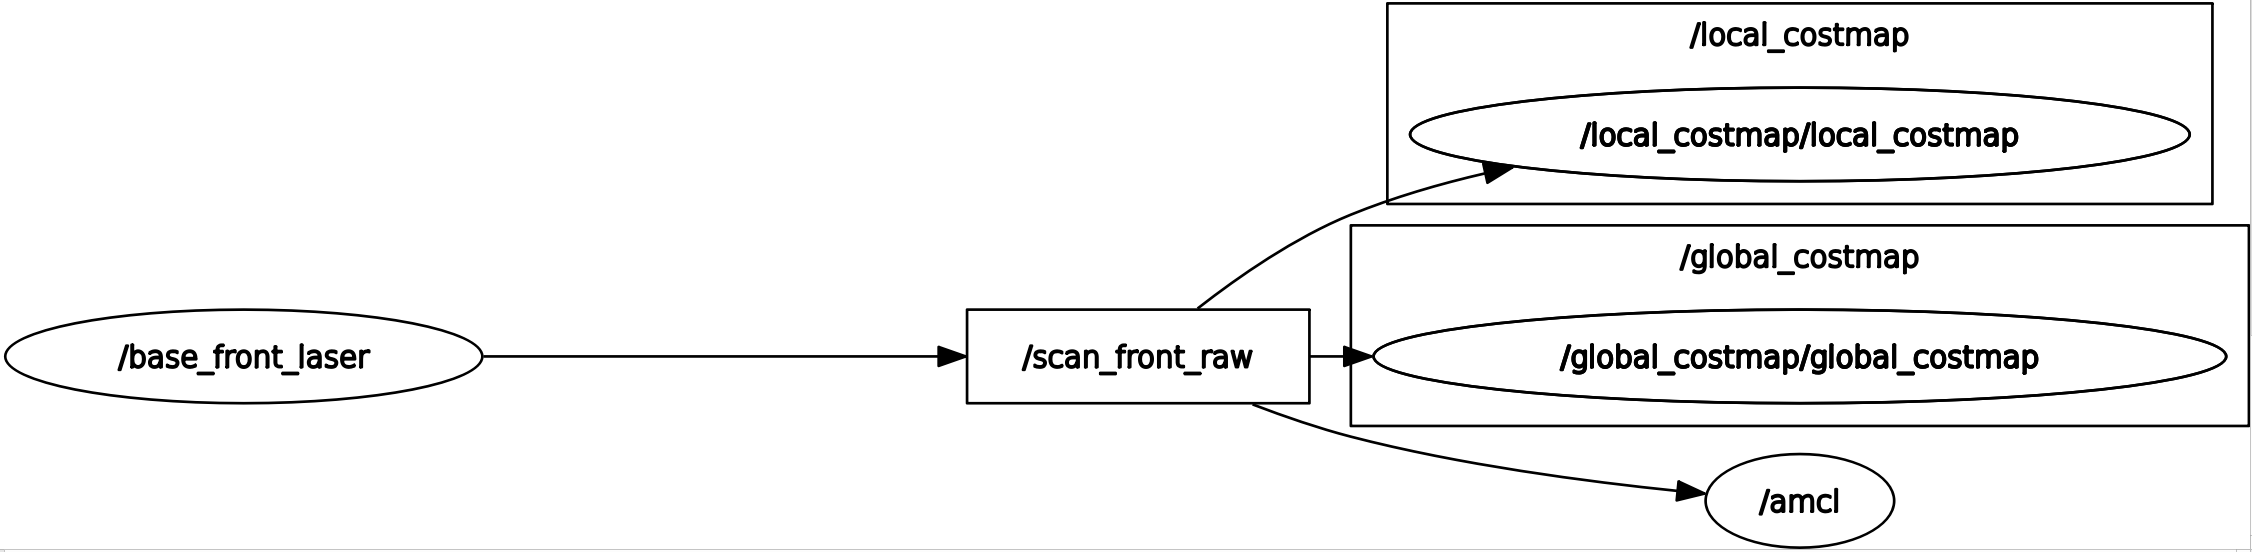
\includegraphics[width=1\textwidth]{images/Ch3/rosgraph_scan_front.png}\\[0.3cm]
    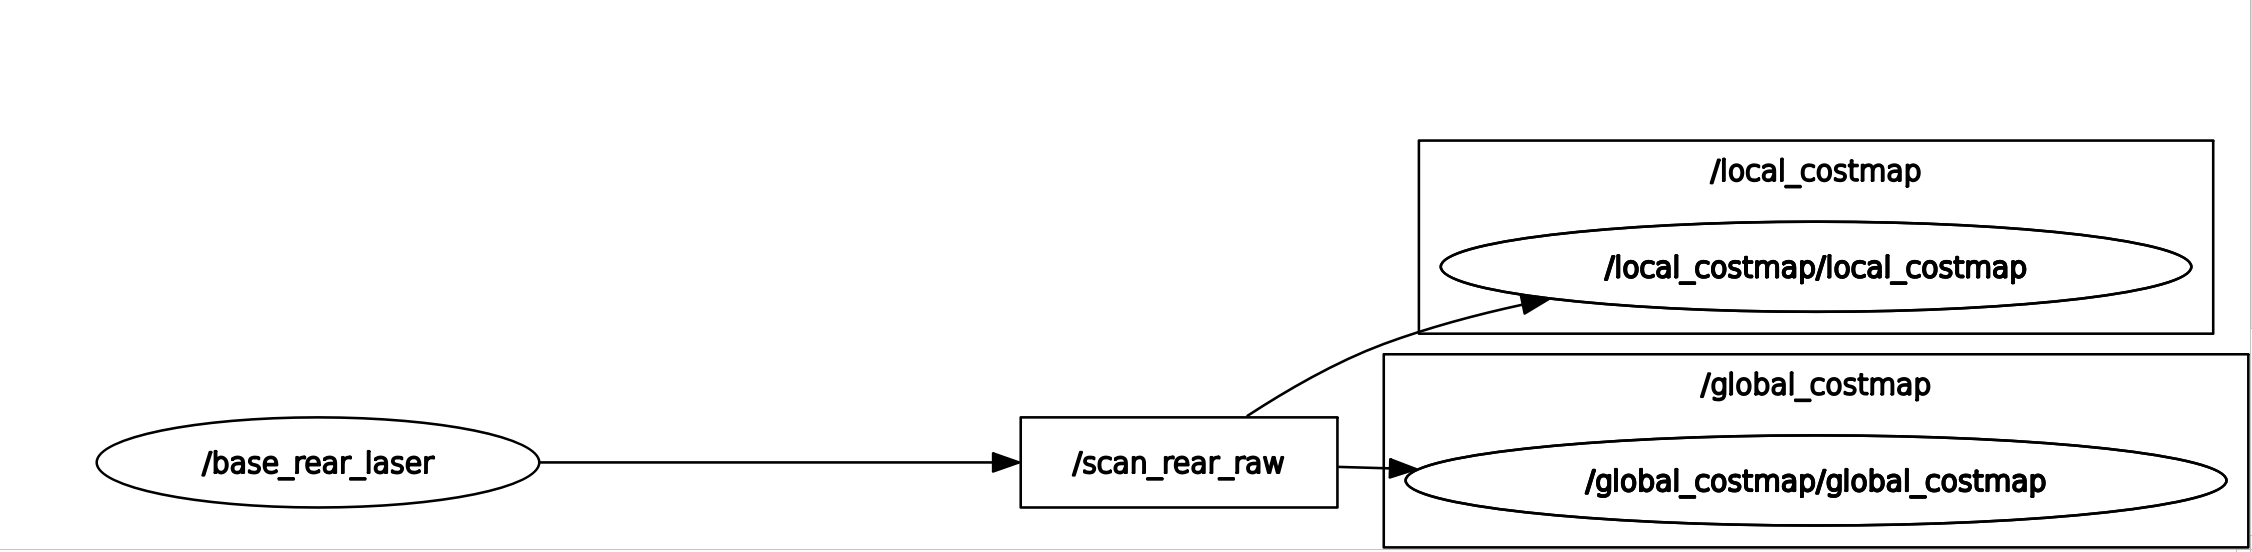
\includegraphics[width=1\textwidth]{images/Ch3/rosgraph_scan_rear.png}
    \caption{Data flow graphs of the OmniBase LiDAR sensors generated via \texttt{rqt\_graph}. Top: The front laser data is ingested by both the costmaps and the AMCL node. Bottom: The rear laser data is exclusively fused into the costmaps for 360-degree obstacle avoidance.}
    \label{fig:laser_graphs}
\end{figure}

Beyond obstacle avoidance, this sensory divergence heavily impacted the Adaptive Monte Carlo Localization (AMCL) system. By default, the PMB2 localization is governed by the \texttt{nav2\_amcl::DifferentialMotionModel}. To properly localize the holonomic base, the robot model type was explicitly switched to the \texttt{nav2\_amcl::OmniMotionModel}. 

This algorithmic switch requires a direct application of the probabilistic theories discussed in Section \ref{sec:probabilistic_motion_models}. In the differential model, the odometric noise is governed by four coefficients ($\alpha_1$ through $\alpha_4$), which model the variance of rotation and longitudinal translation. However, the Mecanum rollers of the OmniBase introduce continuous, controlled lateral slippage. To prevent the particle filter from diverging during lateral translations, the \texttt{alpha5} parameter was introduced into the AMCL configuration. As documented in the configuration files (provided in Appendix \ref{app:nav2_params}), \texttt{alpha5} was set to $0.2$, explicitly bounding the lateral variance ($\sigma^2_y$) and ensuring that the localization filter remained robust even during pure lateral strafing.

It is worth noting that the general holonomic odometry model derived in Section \ref{subsec:holonomic_uncertainty} employs nine coefficients ($\alpha_1$--$\alpha_9$) to describe the fully coupled error propagation across the $x$, $y$, and $\theta$ axes. The \texttt{nav2\_amcl::OmniMotionModel} implements a reduced, five-parameter form of this model ($\alpha_1$ -$\alpha_5$): the four differential coefficients $\alpha_1$--$\alpha_4$ are retained, and the additional $\alpha_5$ term accounts for the lateral (strafing) noise that the differential model omits. This reduced parameterisation is adequate in practice, since the dominant new contribution introduced by holonomic motion is precisely the lateral variance $\sigma_y^2$.

\subsection{Kinematic Constraints and Costmap Adaptation}
\label{subsec:costmap_tuning}

In the Nav2 architecture, the raw velocity commands generated by the local planner are not sent directly to the hardware base. Instead, they are routed through the \texttt{velocity\_smoother} node, which enforces strict kinematic limits, acceleration profiles, and deadbands. 

In the default PMB2 configuration, this smoother acts as a hard kinematic gatekeeper, strictly enforcing non-holonomic constraints. As documented in the configuration files (Appendix \ref{app:nav2_params}), the lateral component of the velocity limits for the differential base is explicitly clamped to zero (\texttt{max\_velocity: [1.0, 0.0, 1.0]} and \texttt{min\_velocity: [-1.0, 0.0, -1.0]}, the central entry being $v_y$). Consequently, even if a generic local planner attempted to output a lateral translation, the smoother would truncate the $v_y$ component, forcing the robot into a purely differential behavior. To physically unlock the kinematics for the OmniBase, these limits were symmetrically expanded (\texttt{max\_velocity: [1.0, 1.0, 1.0]} and \texttt{min\_velocity: [-1.0, -1.0, -1.0]}). Crucially, the minimum $X$ velocity was intentionally maintained at $-1.0$ across both platforms, rather than $0.0$, to ensure that the Nav2 \texttt{BackUp} recovery behavior could still operate effectively during collision avoidance.

Beyond velocity constraints, the geometric representation of the robot within the environment required a fundamental adaptation. The PMB2 operates with a perfectly circular static footprint, defined in both the \texttt{local\_costmap} and \texttt{global\_costmap} by a \texttt{robot\_radius} of $0.275$ meters. A circular footprint is computationally lightweight because its collision bounds are rotationally invariant. 

Conversely, the OmniBase necessitates a rectangular footprint (Figure~\ref{fig:footprints_rviz}) to accurately encapsulate its chassis and Mecanum wheels. The configuration was therefore modified from a scalar radius to a definitive polygon: \texttt{footprint: "[[0.35, 0.24], [-0.35, 0.24], [-0.35, -0.24], [0.35, -0.24]]"}. Introducing a rectangular footprint fundamentally alters the inflation layers and collision-checking heuristics of the costmaps. Because the corners of the rectangle extend further from the geometric center than the lateral sides, the local planner must strictly evaluate the robot's orientation relative to nearby obstacles, particularly during diagonal or pure lateral strafing maneuvers. To maintain adequate safety margins across both kinematics, the \texttt{inflation\_radius} in the local costmap was standardized to $0.55$ meters.

\begin{figure}[H]
    \centering
    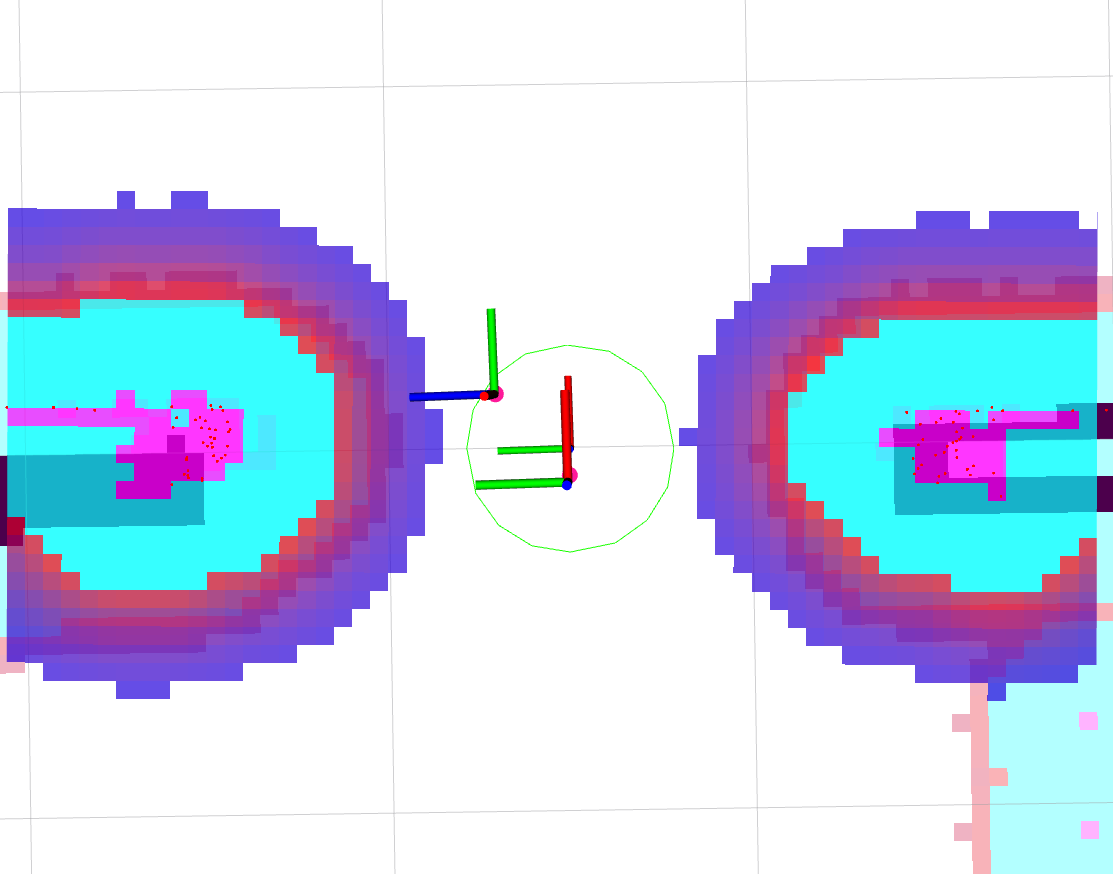
\includegraphics[width=0.48\textwidth]{images/Ch3/footprint_diff.png}
    \hfill
    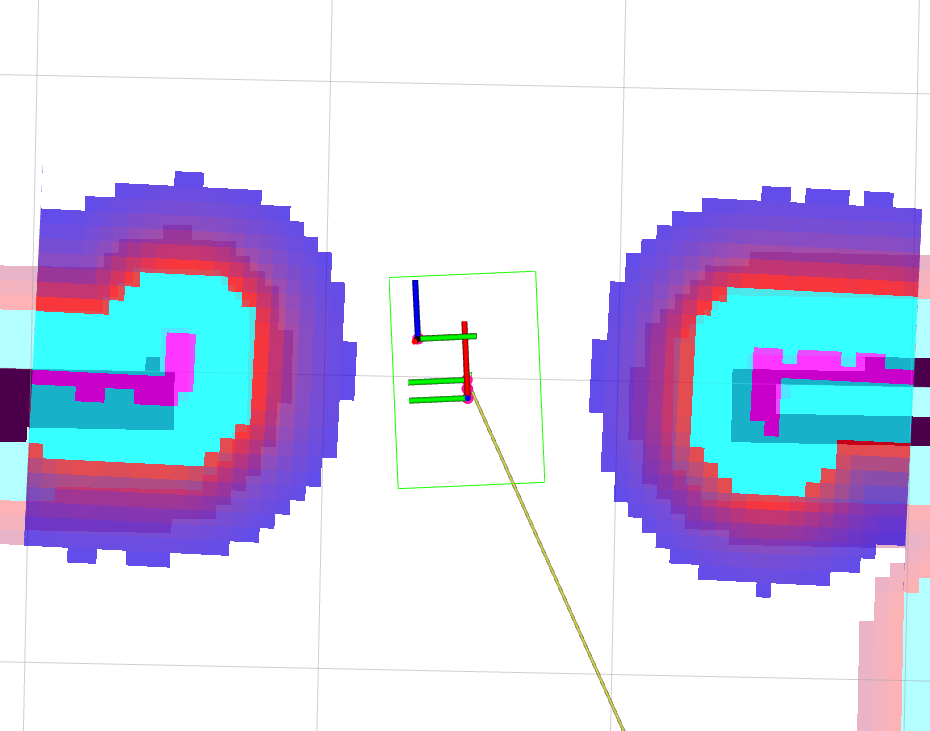
\includegraphics[width=0.48\textwidth]{images/Ch3/footprint_omni.png}
    \caption{Visualization of the local costmap and robot footprints in RViz located in a door. Left: The rotation-invariant circular footprint of the PMB2. Right: The rectangular footprint of the OmniBase.}
    \label{fig:footprints_rviz}
\end{figure}

\subsection{Overcoming the Differential Bias in the Local Planner}
\label{subsec:dwb_tuning}

The most significant architectural hurdle in deploying a holonomic robot within Nav2 lies in the interaction between the global and local planners. By default, the \texttt{NavfnPlanner} computes the optimal geometric path and automatically assigns an orientation to each intermediate pose that is strictly tangent to the trajectory. This inherently imposes a differential-drive advancement logic, dictating that the robot must continuously point its front face towards the direction of travel. 

The \texttt{DWBLocalPlanner} evaluates the feasibility of these trajectories using a set of cost functions known as \textit{Critics}. In the PMB2 baseline configuration, critics such as \texttt{PathAlign} and \texttt{GoalAlign} are heavily weighted (\texttt{scale: 32.0} and \texttt{24.0}, respectively). These critics heavily penalize any movement where the robot's heading does not match the trajectory tangent, effectively forcing the robot to rotate before translating. If applied to the OmniBase, this differential bias overrides its holonomic capabilities, resulting in sub-optimal, parabolic trajectories.

To unlock true omnidirectional movement—specifically, pure lateral translation or \textit{crab walking}—the critics evaluating the robot's heading were radically retuned. For the OmniBase, the weights of \texttt{PathAlign} and \texttt{GoalAlign} were strictly reduced to $0.0$ and $0.0$ (the complete configuration of the retuned Critics is detailed in Appendix \ref{app:dwb_tuning}). By suppressing the obligation to "look ahead", the planner is freed to command lateral velocities ($v_y \neq 0$) while maintaining the initial orientation. For these lateral commands to be resolved with sufficient granularity, the number of velocity samples along the $y$ axis was raised from the differential default (\texttt{vy\_samples: 5}) to \texttt{vy\_samples: 20}, matching the longitudinal resolution; otherwise the discretised velocity search would explore the lateral dimension too coarsely to yield smooth strafing. To ensure the robot did not drift from the optimal line, the \texttt{PathDist} scale was kept high ($64.0$), anchoring the chassis to the geometric path. 

Furthermore, a new critic, \texttt{Twirling} (\texttt{scale: 20.0}), was introduced to the holonomic configuration. Without orientation constraints, an unpenalized holonomic planner might generate arbitrary in-place rotations during lateral strafing. The \texttt{Twirling} critic actively penalizes unnecessary rotational velocities ($\omega$), forcing the robot to maintain a stable, fixed heading throughout the translation. Finally, matching the footprint adaptation discussed previously, the lightweight \texttt{BaseObstacle} critic used for the PMB2 was replaced with the computationally rigorous \texttt{ObstacleFootprint} critic, ensuring collision evaluations were strictly based on the actual rectangular polygon rather than an inscribed radius.

From an automation engineering perspective, forcing the OmniBase into a pure \textit{crab walk} provides two critical operational advantages:
\begin{enumerate}
    \item \textbf{Minimization of Swept Volume:} Pure translation maintains the robot's dynamic footprint strictly equal to its static footprint. By eliminating the need for parabolic turning and in-place rotations, the swept volume is drastically reduced, enabling safer and highly efficient navigation in cluttered or narrow environments.
    \item \textbf{Payload and Perception Stability:} By decoupling the chassis orientation from the velocity vector, the robot can maintain a continuous, fixed viewpoint on a target (e.g., keeping head-mounted optical sensors focused) or carry a manipulated payload steadily without requiring high-frequency compensatory movements from the upper-body joints.
\end{enumerate}

\subsection{Methodological Fairness and Configuration Summary}
\label{subsec:fairness_summary}

A critical methodological declaration must be made regarding the comparative validity of this experimental setup. In robotic benchmarking, applying an identical configuration file to fundamentally distinct hardware platforms does not guarantee an objective comparison; rather, it forces one platform to operate under the physical paradigms of the other. 

To ensure true methodological fairness, each base was explicitly tuned to exploit its own specific kinematics. As summarized in Table \ref{tab:nav2_params}, parameters directly related to the controllable degrees of freedom (such as lateral velocity limits) and heuristic orientation critics (\texttt{PathAlign}, \texttt{GoalAlign}, and \texttt{Twirling}) deliberately differ between the configurations. These kinematic-specific divergences were implemented by design to eliminate the differential bias and unlock the OmniBase's capabilities. 

Conversely, to prevent incidental misalignments from skewing the results, all hardware-agnostic parameters—including maximum linear and angular velocities, acceleration profiles, inflation radii, and path-tracking weights (\texttt{PathDist})—were strictly standardized across both bases. By isolating the parameters in this manner, it is guaranteed that the performance differences observed in the subsequent experimental campaigns derive exclusively from the underlying kinematic properties and the resulting navigation strategies, rather than from arbitrary configuration noise.

\begin{table}[htbp]
    \centering
    \renewcommand{\arraystretch}{1.3}
    \caption{Summary of critical Nav2 parameters highlighting the intentional divergences and standardized similarities between the PMB2 and OmniBase configurations.}
    \vspace{0.2cm}
    \label{tab:nav2_params}
    \begin{tabularx}{\textwidth}{@{} l l l >{\raggedright\arraybackslash}X @{}}
        \toprule
        \textbf{Parameter Name} & \textbf{PMB2 (Diff)} & \textbf{OmniBase (Omni)} & \textbf{Rationale} \\
        \midrule
        \multicolumn{4}{c}{\textbf{Kinematic-Specific Parameters (Tuned by Design)}} \\
        \midrule
        Lateral Vel ($v_y$) & \texttt{[0.0, 0.0]} & \texttt{[-1.0, 1.0]} & Unlocks lateral strafing ($Y$-axis). \\
        Velocity Samples ($v_y$) & \texttt{5} & \texttt{20} & Finer lateral sampling for smooth strafing. \\
        Footprint Geometry & \texttt{radius: 0.275} & \texttt{polygon: [...]} & Matches physical chassis geometry. \\
        \texttt{PathAlign} Critic & \texttt{scale: 32.0} & \texttt{scale: 0.0} & Suppresses forward-heading bias. \\
        \texttt{GoalAlign} Critic & \texttt{scale: 24.0} & \texttt{scale: 0.0} & Decouples orientation from motion. \\
        \texttt{Twirling} Critic & Not utilized & \texttt{scale: 20.0} & Penalizes arbitrary spin during strafe. \\
        AMCL Motion Model & \texttt{Differential} & \texttt{OmniMotion} & Matches probabilistic mechanics. \\
        AMCL \texttt{alpha5} Noise & Not evaluated & \texttt{0.2} & Bounds lateral slippage variance. \\
        \midrule
        \multicolumn{4}{c}{\textbf{Identical Parameters (Standardized Baseline)}} \\
        \midrule
        Max Vel ($v_x$, $\omega$) & \texttt{1.0, 1.0} & \texttt{1.0, 1.0} & Standardized absolute speed limits. \\
        Max Accel ($a_x$, $a_\omega$) & \texttt{2.5, 3.2} & \texttt{2.5, 3.2} & Standardized dynamic constraints. \\
        \texttt{PathDist} Critic & \texttt{scale: 64.0} & \texttt{scale: 64.0} & Equal adherence to global trajectory. \\
        \texttt{GoalDist} Critic & \texttt{scale: 24.0} & \texttt{scale: 24.0} & Equal attraction to the final goal. \\
        \texttt{inflation\_radius} & \texttt{0.55} & \texttt{0.55} & Consistent obstacle safety margin. \\
        AMCL $\alpha_1 - \alpha_4$ & \texttt{0.2} & \texttt{0.2} & Consistent base odometric noise. \\
        \bottomrule
    \end{tabularx}
\end{table}
%!TeX root = ../main.tex

% ==========================================
% CHAPTER 4: EXPERIMENTAL RESULTS AND COMPARISON
% ==========================================
\chapter{Experimental Results and Comparison}
\label{ch:results}

Chapters~\ref{Ch:Kinematic} and~\ref{ch:architecture} established, respectively, the kinematic models of the two platforms and the software architecture required to deploy them fairly within the ROS~2 Nav2 stack. This chapter presents the experimental validation of that architecture and the quantitative comparison between the differential PMB2 and the holonomic OmniBase. The evaluation spans the two navigation pipelines that motivate this work: directed waypoint navigation across three topological challenges, and autonomous frontier-based exploration of an unknown domestic environment. Each scenario was repeated for five iterations per base, and all spatial quantities were computed offline from absolute Ground Truth poses, so that the observed differences can be attributed to the underlying kinematics and the resulting navigation strategies rather than to onboard estimation noise. The chapter first describes the simulation environments and experimental protocols (Section~\ref{sec:exp-setup}) and the evaluation metrics together with their methodological caveats (Section~\ref{sec:eval-metrics}); it then reports the waypoint and exploration results (Sections~\ref{sec:wp-results} and~\ref{sec:expl-results}) and closes with a cross-paradigm synthesis (Section~\ref{sec:comparative-discussion}).

\section{Experimental Setup}
\label{sec:exp-setup}

The experimental campaigns were conducted entirely in simulation, relying on the Gazebo Classic worlds and the deterministic launch infrastructure detailed in Chapter~\ref{ch:architecture}. This section introduces the two simulation scenarios (Section~\ref{subsec:sim-scenarios}) and the two experimental protocols used to benchmark the platforms: directed waypoint navigation (Section~\ref{subsec:wp-protocol}) and autonomous exploration (Section~\ref{subsec:expl-protocol}).

\subsection{Simulation Scenarios}
\label{subsec:sim-scenarios}

Two distinct Gazebo Classic worlds were employed (Figure~\ref{fig:sim-worlds}), each tailored to one of the two navigation pipelines. Both environments were instrumented with the \texttt{gazebo\_ros\_state} plugin introduced in Section~\ref{subsec:simulation_gt}, which publishes the absolute pose of the robot at 50~Hz and provides the Ground Truth reference used throughout the offline analysis.

The directed waypoint-navigation campaign was executed in the PAL Robotics  \\ \texttt{small\_office} world, a structured indoor environment. As detailed in Section~\ref{subsec:simulation_gt}, this stock world was adapted for benchmarking by adjusting the lighting, removing overhanging desks that produced blind collisions above the LiDAR plane, and populating the space with static human models to emulate a realistic, cluttered office. Its regular geometry makes it well suited to controlled and repeatable path-following tests, since the three waypoint routes (Section~\ref{subsec:wp-protocol}) can be arranged to isolate specific navigational challenges---a straight corridor, a sharp corner, and a densely obstructed passage.

The autonomous-exploration campaign was instead conducted in the \texttt{home} world, a realistic domestic apartment comprising multiple connected rooms. In contrast to the office, this environment was deliberately left unaltered in order to preserve a highly complex and representative scenario. Because the exploration task requires the robot to incrementally discover an initially unknown map, the larger scale and irregular room topology of the apartment provide a demanding setting in which to compare the two kinematics under simultaneous localisation and mapping.

\begin{figure}[H]
    \centering
    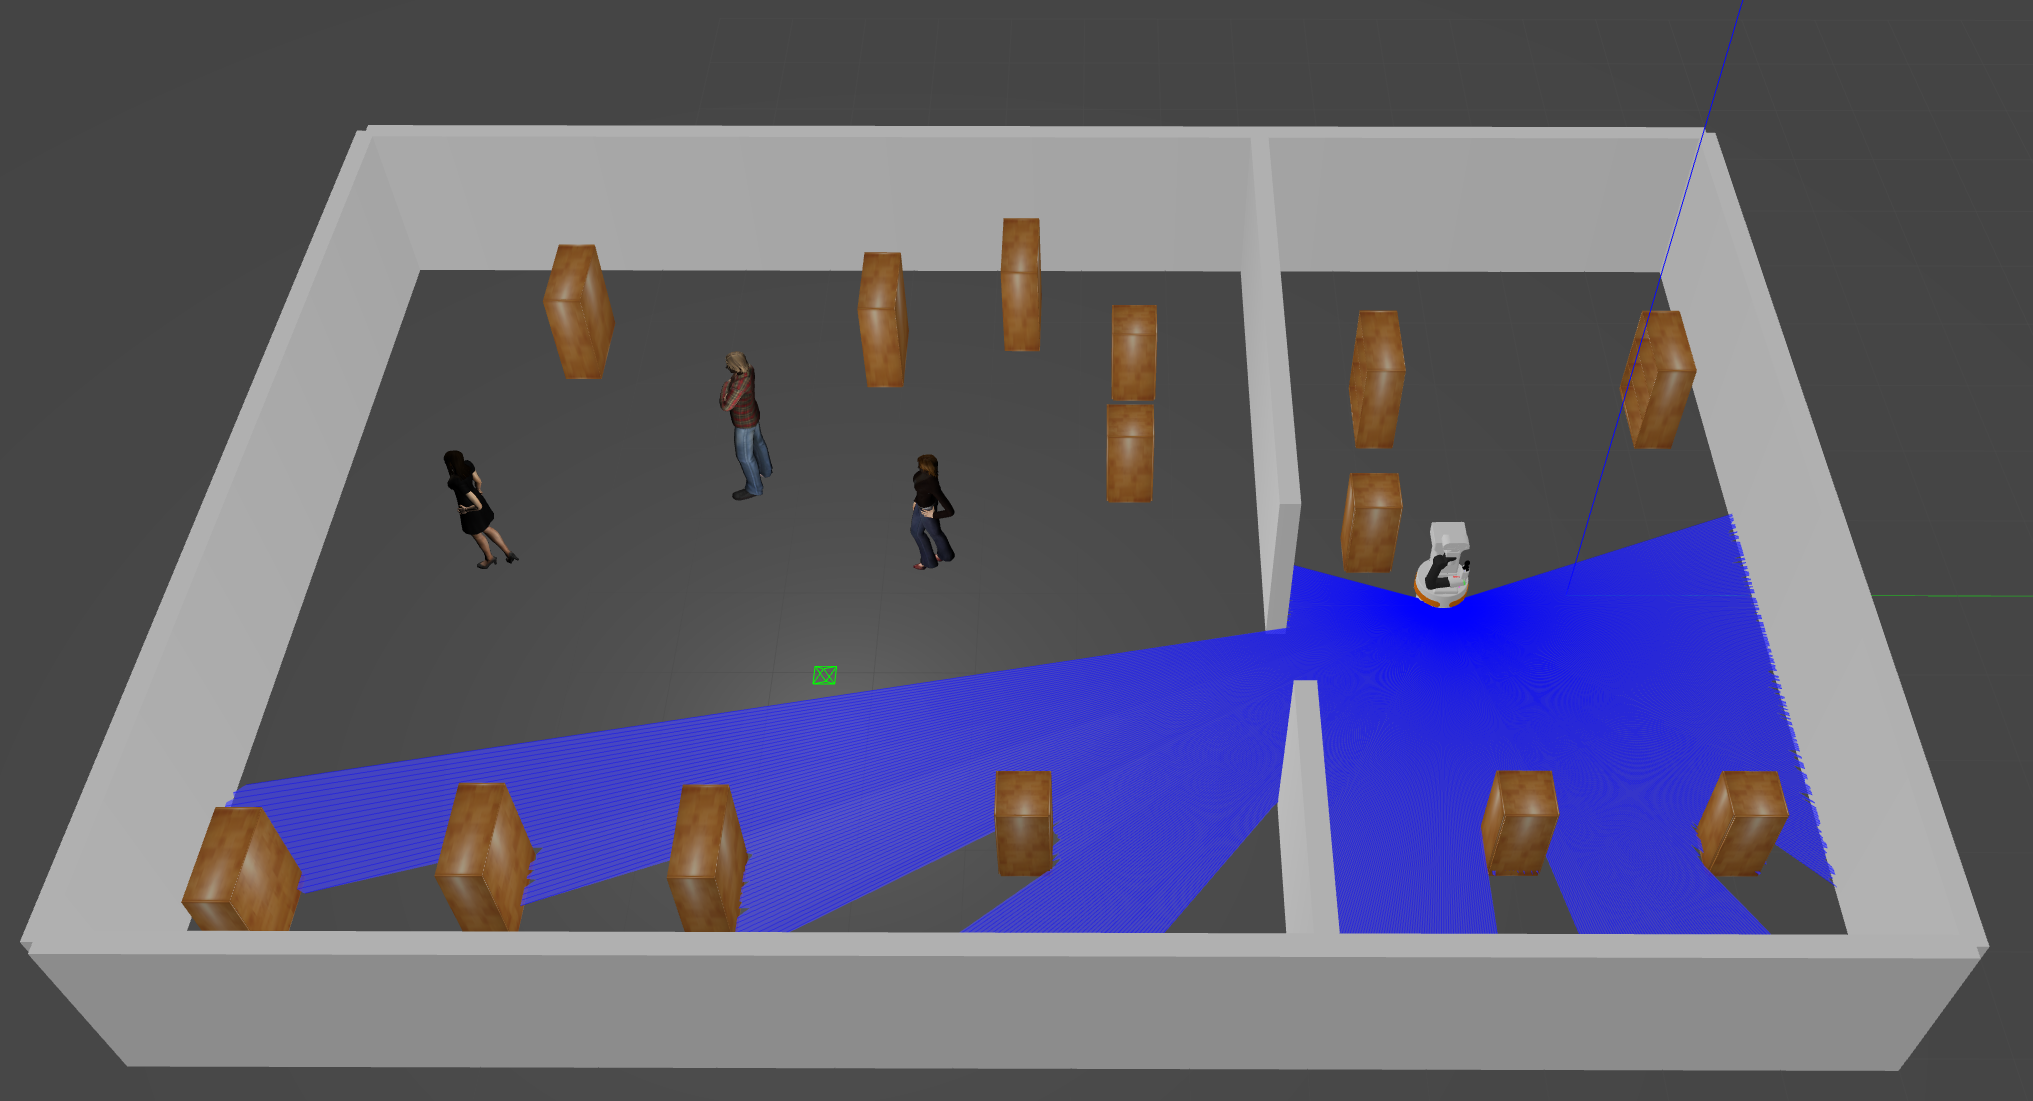
\includegraphics[width=0.49\textwidth]{images/Ch4/Small_office_diff.png}
    \hfill
    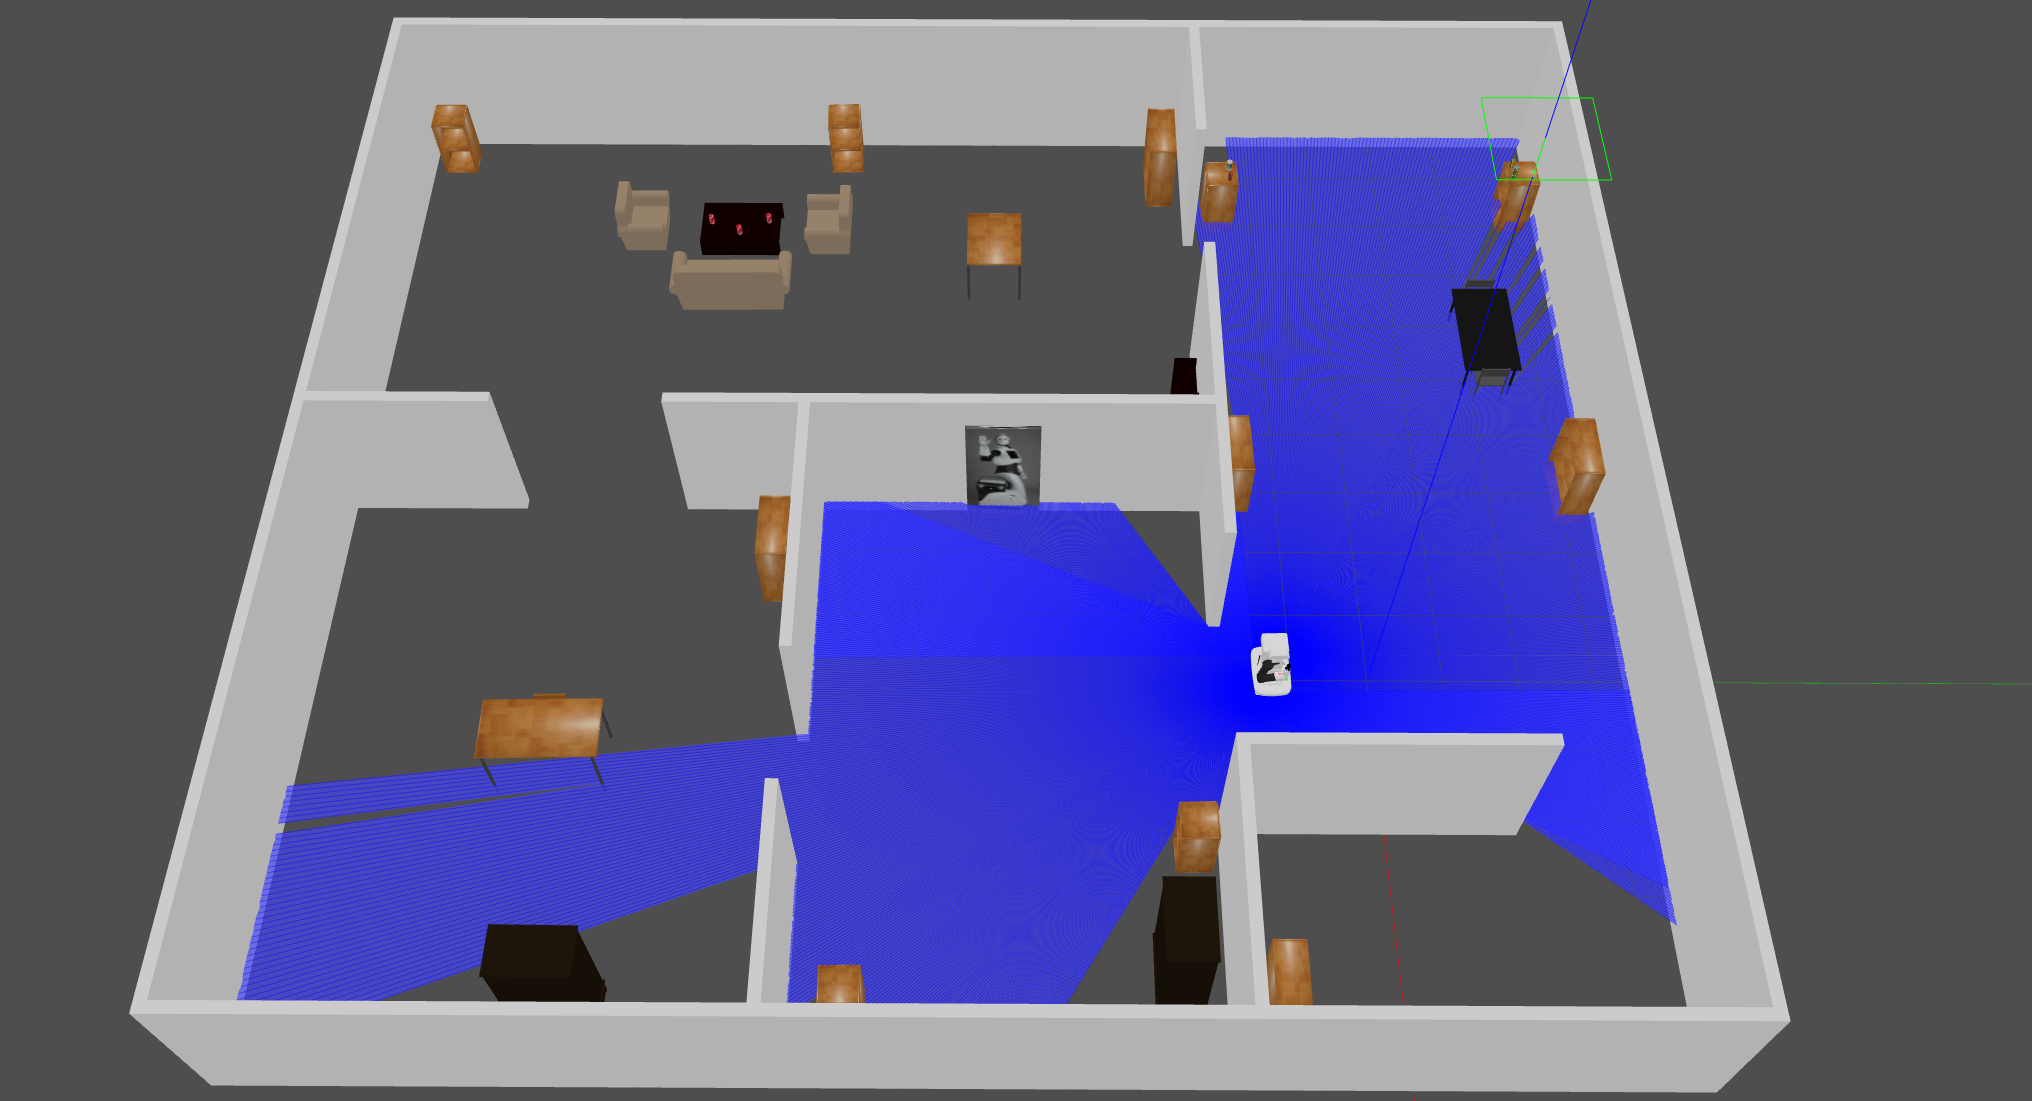
\includegraphics[width=0.49\textwidth]{images/Ch4/Home_omni.png}
    \caption{The two Gazebo Classic simulation environments. Left: the modified \texttt{small\_office} world used for the waypoint-navigation campaign, populated with static obstacles and human models. Right: the unaltered \texttt{home} apartment used for the autonomous-exploration campaign.}
    \label{fig:sim-worlds}
\end{figure}

\subsection{Waypoint Navigation Protocol}
\label{subsec:wp-protocol}

The first pipeline evaluates directed point-to-point navigation on a previously mapped environment. The robot was commanded to traverse an ordered sequence of poses through the Nav2 \texttt{NavigateThroughPoses} action, dispatched from a custom driver node built on the \\ \texttt{nav2\_simple\_commander} API (the driver and the Ground~Truth logging node are documented in Appendix~\ref{app:results_scripts}). Unlike a series of independent \texttt{NavigateToPose} goals, this action plans a single continuous path through all the intermediate poses without requiring the robot to stop at each one. Consequently, the intermediate waypoints behave as positional via-points that the trajectory is only required to approach within tolerance, leaving the platform free to smooth the path---most notably by cutting corners---rather than pausing and re-orienting at every pose. Moreover, only the orientation of the final pose is enforced: the headings assigned to the intermediate waypoints are not actively pursued. This behaviour is central to the correct interpretation of the positioning and orientation errors and is discussed further in Section~\ref{sec:eval-metrics}.

Three routes of increasing difficulty were designed within the \texttt{small\_office} world, each isolating a distinct navigational challenge. Their exact coordinates are reported in Appendix~B.

\textbf{Path~A --- Straight Corridor.} A two-waypoint route consisting of a single rectilinear segment, approximately $13$~m long, running along a straight corridor of the office (Figure~\ref{fig:hallway_traj}). With no turns or obstacles, this path isolates pure path-following and steady-state velocity behaviour, and serves as the baseline against which the two kinematics are first compared.

\textbf{Path~B --- Sharp Corner.} A four-waypoint route describing an ``L''-shaped trajectory: a $1.5$~m segment followed by a sharp $90^{\circ}$ turn and a further $1.3$~m segment, for a total reference length of $2.8$~m. This deliberately short route stresses the platforms' response to an abrupt change of direction, contrasting the in-place rotation required by the differential drive with the lateral strafing available to the holonomic one.

\textbf{Path~C --- Cluttered Obstacle Course.} An eleven-waypoint route, approximately $25.9$~m long, winding through the populated office and passing in close proximity to two static human models. By repeatedly forcing the global planner to compute paths through narrow, obstructed passages, this route most severely stresses the planning stack and is expected to expose the differences in navigation robustness between the two bases.

All three routes begin at the spawn pose (waypoint~$0$), so that every run starts from the precise coordinates enforced by the deterministic initialisation routine of Section~\ref{subsec: Deterministic Init}. The positioning error at this first waypoint is therefore null by construction and is disregarded when interpreting the results, which focus instead on the intermediate waypoints and the final goal. Each route was executed five times per base, yielding a total of $30$ waypoint-navigation runs ($2$ bases $\times$ $3$ routes $\times$ $5$ repetitions). During every run, the absolute Ground~Truth pose was logged at $50$~Hz together with the velocity commands issued by the navigation stack; all metrics and figures were then computed offline over the \emph{active navigation window}---from the instant the first waypoint becomes active until the sequence completes---so as to exclude the initial postural settling at spawn and any idle time after arrival.
\begin{figure}[H]
    \centering
    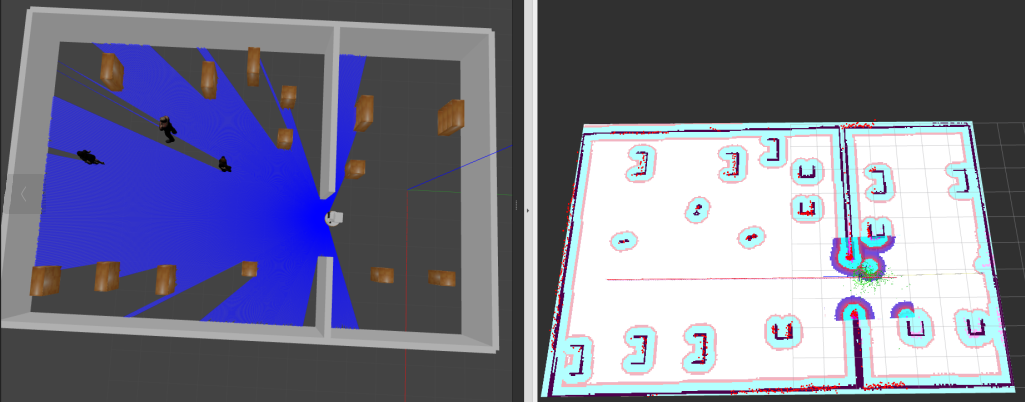
\includegraphics[width=1\textwidth]{images/Ch4/Zoom_Setup_simulazione_hallway.png} 
    \caption{Path~A --- Straight Corridor during simulation}
    \label{fig:hallway_traj}
\end{figure}


\subsection{Autonomous Exploration Protocol}
\label{subsec:expl-protocol}

The second pipeline evaluates autonomous exploration of an initially unknown environment. In contrast to the waypoint campaign, no map is provided in advance: the robot incrementally builds an occupancy grid on-line through \texttt{slam\_toolbox} while Nav2 drives it towards a succession of self-selected goals. This setting exercises the full navigation loop---simultaneous mapping, localisation, global planning, and local control---and is therefore the more demanding test of how each kinematic model copes with a realistic domestic space (the \texttt{home} world of Section~\ref{subsec:sim-scenarios}; Figure~\ref{fig:aut-exp sim}).

Exploration is driven by a custom frontier-based node (documented in Appendix~\ref{app: autonomous expl node}), originally developed during a prior internship and substantially re-instrumented for this thesis to guarantee deterministic and fair comparisons. At each iteration the node analyses the live occupancy grid published by SLAM and identifies the \emph{frontiers}, i.e.\ the cells lying on the boundary between explored free space and still-unknown regions. A single frontier is then selected according to a configurable, deterministic policy and dispatched to Nav2 as a navigation goal, with its orientation set towards the unexplored area so that the robot arrives already facing the region to be scanned. The cycle repeats until the number of residual frontier cells falls below a fixed threshold, at which point the map is considered complete and the robot returns to its starting position.

Deploying a naive frontier explorer on the two platforms would, however, conflate genuine kinematic differences with incidental planner failures. Three heuristics were therefore introduced to keep the comparison fair and repeatable:
\begin{itemize}
    \item \textbf{Goal retraction from unknown boundaries.} A frontier cell lies exactly on the free/unknown border; as the robot approaches it, the laser frequently reveals a wall just beyond the previous sensor horizon, whose inflation then covers the goal and makes the previously valid target unreachable, triggering spurious recovery behaviours. Each goal is therefore pulled back by a fixed distance along the frontier-to-robot direction, so that it falls in already-confirmed free space while the robot still advances towards, and scans, the frontier.
    \item \textbf{Wall-clearance filtering.} Frontiers lying closer than a minimum clearance to an obstacle are discarded a priori, preventing the planner from being sent towards goals trapped inside the costmap inflation layer.
    \item \textbf{Dynamic goal blacklisting.} Any goal rejected or aborted by the planner is added to a blacklist and excluded, together with a surrounding radius, from subsequent selections, which avoids endless recovery loops around a single problematic point.
\end{itemize}

To ensure that both bases were driven by exactly the same exploration logic, all of these parameters were held identical across the two platforms: a nearest-frontier selection policy, a minimum wall clearance of $0.55$~m, a goal retraction of $0.40$~m, a blacklist radius of $1.0$~m, a completion threshold of $10$ residual frontier cells, and a per-goal navigation timeout of $20$~s. Consequently, any difference in the exploration behaviour reflects the underlying kinematics and the response of the shared Nav2 stack, rather than a divergence in the exploration strategy itself.

As in the waypoint campaign, the exploration was repeated five times per base---for a total of $10$ runs---to characterise run-to-run variability, since the interaction between planner, incremental SLAM updates, and goal selection makes each run slightly different even under a deterministic policy. Throughout each run the absolute Ground~Truth pose was logged alongside the SLAM pose estimate and the commanded velocities; the SLAM localisation error, and the map-to-world frame alignment required to compute it fairly for the two bases, are discussed in Section~\ref{sec:eval-metrics}. All metrics were again evaluated over the active exploration window, from the first frontier goal until the completion criterion is met.

\begin{figure}[H]
     \centering
     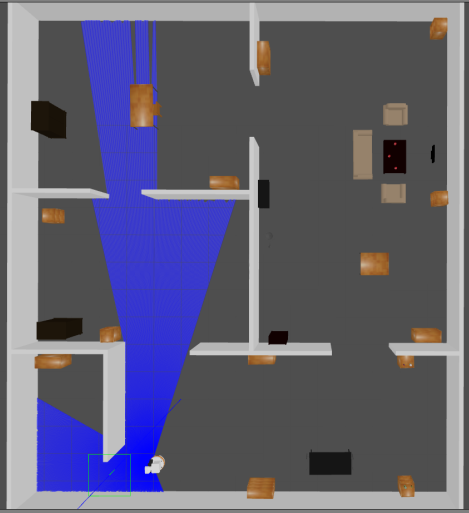
\includegraphics[width=0.45\textwidth]{images/Ch4/zoom_gazebo_aut_exp.png}
     \hfill
     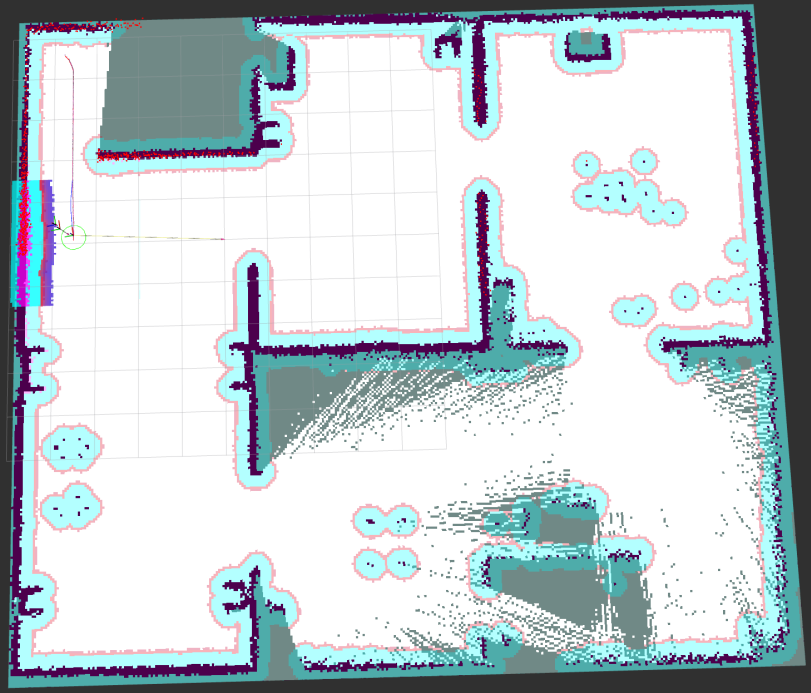
\includegraphics[width=0.5\textwidth]{images/Ch4/zoom_rviz_aut_exp.png}
     \caption{Autonomous Exploration Simulation. Left: Gazebo environment. Right: RViz environment.}
     \label{fig:aut-exp sim}
\end{figure}


\section{Evaluation Metrics}
\label{sec:eval-metrics}

All quantities compared in this chapter were computed offline from the absolute Ground~Truth poses of Section~\ref{subsec:simulation_gt}, not from the robot's own estimate: odometry drifts without bound and AMCL adds model-dependent noise, so evaluating path-following through each base's localisation would confound the kinematic comparison with an estimation artefact. Every metric is evaluated over the active navigation window and, unless stated otherwise, reported as mean $\pm$ standard deviation over the five repetitions of each configuration. The following subsections define the accuracy (Section~\ref{subsec:m-accuracy}), efficiency and motion-quality (Section~\ref{subsec:m-efficiency}), and robustness (Section~\ref{subsec:m-robustness}) metrics, the exploration-specific metrics (Section~\ref{subsec:m-exploration}), and the simulation-fidelity considerations that frame the fairness of the comparison (Section~\ref{subsec:m-fidelity}).

\subsection{Trajectory and Path-Following Accuracy}
\label{subsec:m-accuracy}

The \emph{path length} is the arc length of the Ground~Truth trajectory over the active window; the \emph{reference length} is the sum of the straight segments joining all waypoints. The two need not coincide---cutting corners shortens the path, detouring around obstacles lengthens it---so the reference is a descriptive baseline, not an optimum, and is read together with the tracking error.

The \emph{tracking error} measures how faithfully a base follows the planned trajectory: for each Ground~Truth sample it is the perpendicular distance to the Nav2 global plan (\texttt{/plan}) of the \emph{leg} active at that instant---a leg being the stretch of route between two consecutive waypoints---summarised by its mean, maximum, and root-mean-square. The plan is used as reference---rather than a straight waypoint-to-waypoint line---because it already embeds the planner's \\ obstacle-avoidance detours, so the deviation from it answers the meaningful question of how closely the base executed the path it was actually given. For each leg the reference is the plan published at the start of that leg, reconstructed offline from the recorded rosbag; on the rare legs without an available plan, the analysis falls back to the straight segment and flags the substitution.

The \emph{waypoint positioning error} is the \emph{closest-approach} distance between the trajectory and each waypoint. Because \texttt{NavigateThroughPoses} yields a single fluid trajectory that does not stop at the intermediate poses (Section~\ref{subsec:wp-protocol}), this definition is preferred over the pose sampled at the index switch for three reasons:
\begin{enumerate}
    \item \textbf{Robustness to skipped indices.} A fast base can retire two poses within one feedback cycle, so an intermediate index is never published---as for the OmniBase on Path~B---leaving an index-based rule undefined, whereas the closest approach is always well defined.
    \item \textbf{Honest meaning at pass-through waypoints.} It equals exactly how far the trajectory passed from the point, i.e.\ the corner-cutting distance.
    \item \textbf{Consistency at the goal.} At the final stop it coincides with the final positioning error, free of the timing noise of an arbitrary sampling instant.
\end{enumerate}
The error at the first waypoint, where the robot spawns, is close to zero by construction (up to a small residual reflecting the initial placement) and is not analysed further.

The \emph{orientation error}, evaluated at the point of closest approach, requires care. With \texttt{NavigateThroughPoses} only the final orientation is enforced, so the intermediate waypoint headings are decorative and the error there is measured against a target never pursued; moreover, at a pass-through waypoint the heading equals the instantaneous direction of motion, so a differential base---which must rotate in order to translate---is constantly re-orienting and shows large intermediate errors, while a holonomic base holds a fixed heading while strafing. The intermediate orientation error is therefore read as an indicator of heading stability, and only the error at the final goal, where the heading is genuinely commanded, measures final angular accuracy.

\subsection{Efficiency and Motion Quality}
\label{subsec:m-efficiency}

The \emph{completion time} is the duration of the active window, measured in simulated time, and the \emph{average speed} is the path length divided by it. Relying on simulated time makes the results independent of the simulation's real-time factor (RTF), which was not strictly below unity---on the short Path~B runs it reached $1.02$--$1.21$---and which enforcing \texttt{use\_sim\_time} across the pipeline (Section~\ref{subsec:gpu optimization}) renders irrelevant to the comparison: all nodes share Gazebo's \texttt{/clock}, so durations stay consistent regardless of how fast the simulation ran on the wall clock.

\emph{Motion smoothness} is quantified as the root-mean-square of the commanded acceleration, obtained by numerically differentiating the linear and angular velocity commands issued on \texttt{/cmd\_vel}; a lower value denotes smoother motion. It is computed from the commands, rather than from the Ground~Truth trajectory, so that it reflects the control effort requested by the planner, and it is reported separately as a linear and an angular component (\texttt{smooth\_lin}, \texttt{smooth\_ang}).

Finally, the \emph{lateral usage} is the fraction of the motion performed through the lateral (strafing) velocity component: zero by construction for the differential base, which cannot translate sideways, and positive for the holonomic one, it directly measures how much each platform exploited its available degrees of freedom.

\subsection{Robustness}
\label{subsec:m-robustness}

Navigation robustness is assessed primarily through the \emph{planning failures}: the number of times the global planner failed to produce a valid path, and the corresponding \emph{failure rate}, i.e.\ failures over planning attempts. This is the metric on which the two kinematics differ most sharply, the differential base repeatedly failing to plan around obstacles where the holonomic one does not.

Complementing it, the \emph{recovery behaviours} count the Nav2 recovery actions triggered when normal planning or control stalls---rotating in place (Spin), reversing (BackUp), waiting (Wait), and costmap clearing (ClearCostmap). Costmap clearing is the most frequent around obstacles and, in the Nav2 behaviour tree, is invoked by a planning failure before the next attempt; the spatial location of these clears therefore marks where planning struggled, which motivates the recovery maps shown in the results.

A further quantity, the number of \emph{replans}, is reported only for completeness: replanning is issued periodically at roughly $1$~Hz, so its count scales with run duration rather than with difficulty, and it is treated as a secondary, bookkeeping quantity rather than a headline indicator. All of the above counts were extracted offline from the recorded rosbags by parsing the \texttt{/behavior\_tree\_log} topic and counting each behaviour's activations---a single, uniform source across both pipelines, which also correctly captures one-shot actions such as costmap clearing.

\subsection{Exploration-Specific Metrics}
\label{subsec:m-exploration}

The exploration task is characterised by a dedicated set of metrics, alongside the smoothness, lateral-usage, and robustness quantities already defined, which apply unchanged. The \emph{final mapped area} is the free area of the occupancy grid at the end of the run, and the \emph{exploration time} is the duration of the active exploration window. To compare runs that terminate with slightly different coverage, the \emph{time-to-target} measures the time taken to map a common target area, set to $95\%$ of the smallest final area observed across all runs, so that every run is evaluated at a coverage level all of them attained. Exploration \emph{efficiency} is then expressed both per unit distance (area per metre travelled) and per unit time (area per second).

The \emph{SLAM localisation error} is the distance between the Ground~Truth pose and the pose estimated by \texttt{slam\_toolbox}, summarised by its mean and maximum. Computing it fairly requires aligning the SLAM \texttt{map} frame with the Gazebo \texttt{world} frame, because the two bases operate under different odometric regimes by construction of their simulation plugins: the PMB2 wheel odometry is zeroed at spawn, so its \texttt{map} origin coincides with the spawn pose, whereas the OmniBase is driven by \texttt{gazebo\_ros\_planar\_move}, whose odometry is referenced to the world, so its \texttt{map} origin already coincides with it. Without correction, the PMB2 would exhibit a spurious constant offset---about $1.3$~m, the spawn displacement---that is not a SLAM error. An initial-pose (ATE-style) alignment is therefore estimated from the first valid samples of each run and removed before the error is computed, making the two measurements comparable.

\subsection{Simulation Fidelity and the Fairness of the Comparison}
\label{subsec:m-fidelity}

As anticipated in Section~\ref{subsec:odom tf bridge}, the two bases are actuated differently in simulation, and this asymmetry must be kept in mind when reading the results. The PMB2 is driven through \texttt{ros2\_control}, so its motion follows from an idealised model of the wheel dynamics, whereas the OmniBase is driven by \texttt{gazebo\_ros\_planar\_move}, which imposes the commanded body twist $(v_x, v_y, \omega)$ directly, without any actuation dynamics. As a consequence, the OmniBase follows the velocity commands almost perfectly \emph{by construction}, not because it is inherently a superior platform. The same reasoning applies to the wheel-rotation comparison used in the results: the OmniBase wheel velocities are not measured but reconstructed from the inverse kinematic model of Chapter~\ref{Ch:Kinematic}, whereas the PMB2 wheel rotation is read from the simulator. The comparison nonetheless remains meaningful because both describe an ideal, no-slip rotation---by construction for the OmniBase, and, for the PMB2, effectively so on a flat floor where the simulated wheels barely slip---so the two quantities live in the same idealised kinematic regime rather than reflecting actuation dynamics.

Three implications follow:
\begin{enumerate}
    \item \textbf{Optimistic timing and smoothness.} The holonomic base enjoys a mild optimistic bias on completion time and smoothness, as it executes the acceleration-limited command with no actuation lag; its advantage on these metrics should therefore be read as an upper bound.
    \item \textbf{Understated variance.} Its very low run-to-run variance is partly a plugin effect, and is reported as such rather than claimed as physical stability of the robot.
    \item \textbf{Strategy-level framing.} The comparison is consequently framed at the level of the navigation and planning strategy under different kinematics---the subject of this thesis---rather than as a comparison of physical execution fidelity.
\end{enumerate}
The most trustworthy metrics are thus those independent of actuation fidelity: completion time in simulated units, path shape, the amount of in-place rotation, and lateral usage. For the same reason, the SLAM comparison of Section~\ref{subsec:m-exploration} is best understood as the same SLAM algorithm operating on two different odometric regimes, rather than as a property of the bases in isolation.

\section{Waypoint Navigation Results}
\label{sec:wp-results}

This section reports the results of the waypoint-navigation campaign, presenting the three routes in order of increasing difficulty: the straight corridor (Section~\ref{subsec:res-hallway}), the sharp corner (Section~\ref{subsec:res-angle}), and the cluttered obstacle course (Section~\ref{subsec:res-obstacles}). For each route the two platforms are compared on the metrics defined in Section~\ref{sec:eval-metrics}, aggregated as mean $\pm$ standard deviation over the five repetitions; per-run detail is illustrated using the median run of each base, selected by completion time.

\subsection{Straight Corridor (Path~A)}
\label{subsec:res-hallway}

On the straight corridor both platforms completed all five runs successfully, and neither triggered a single recovery behaviour or planning failure: the route is short and unobstructed, so the navigation stack drives each base to the goal without intervention. Figure~\ref{fig:hallway-traj} shows the Ground~Truth trajectories of all runs, which form a tight bundle along the corridor axis for both bases and confirm the high repeatability of the setup. The aggregate metrics are summarised in Table~\ref{tab:hallway}.

\begin{table}[htbp]
\centering
\caption{Straight corridor (Path~A): aggregate metrics, mean $\pm$ standard deviation over five runs.}
\label{tab:hallway}
\begin{tabular}{lcc}
\toprule
Metric & PMB2 (differential) & OmniBase (holonomic) \\
\midrule
Completion time [s]            & $24.10 \pm 0.52$ & $23.56 \pm 0.14$ \\
Average speed [m/s]            & $0.534 \pm 0.011$ & $0.542 \pm 0.003$ \\
Tracking error, mean [m]      & $0.124 \pm 0.024$ & $0.079 \pm 0.020$ \\
Tracking error, RMS [m]       & $0.147 \pm 0.030$ & $0.100 \pm 0.021$ \\
Goal positioning error [m]    & $0.269 \pm 0.039$ & $0.238 \pm 0.023$ \\
Linear smoothness [m/s$^2$]   & $1.340 \pm 0.058$ & $0.845 \pm 0.081$ \\
Angular smoothness [rad/s$^2$] & $0.614 \pm 0.093$ & $0.611 \pm 0.107$ \\
Lateral usage                  & $0.000 \pm 0.000$ & $0.075 \pm 0.010$ \\
Recoveries / plan failures     & $0$ / $0$ & $0$ / $0$ \\
\bottomrule
\end{tabular}
\end{table}

\begin{figure}[H]
  \centering
  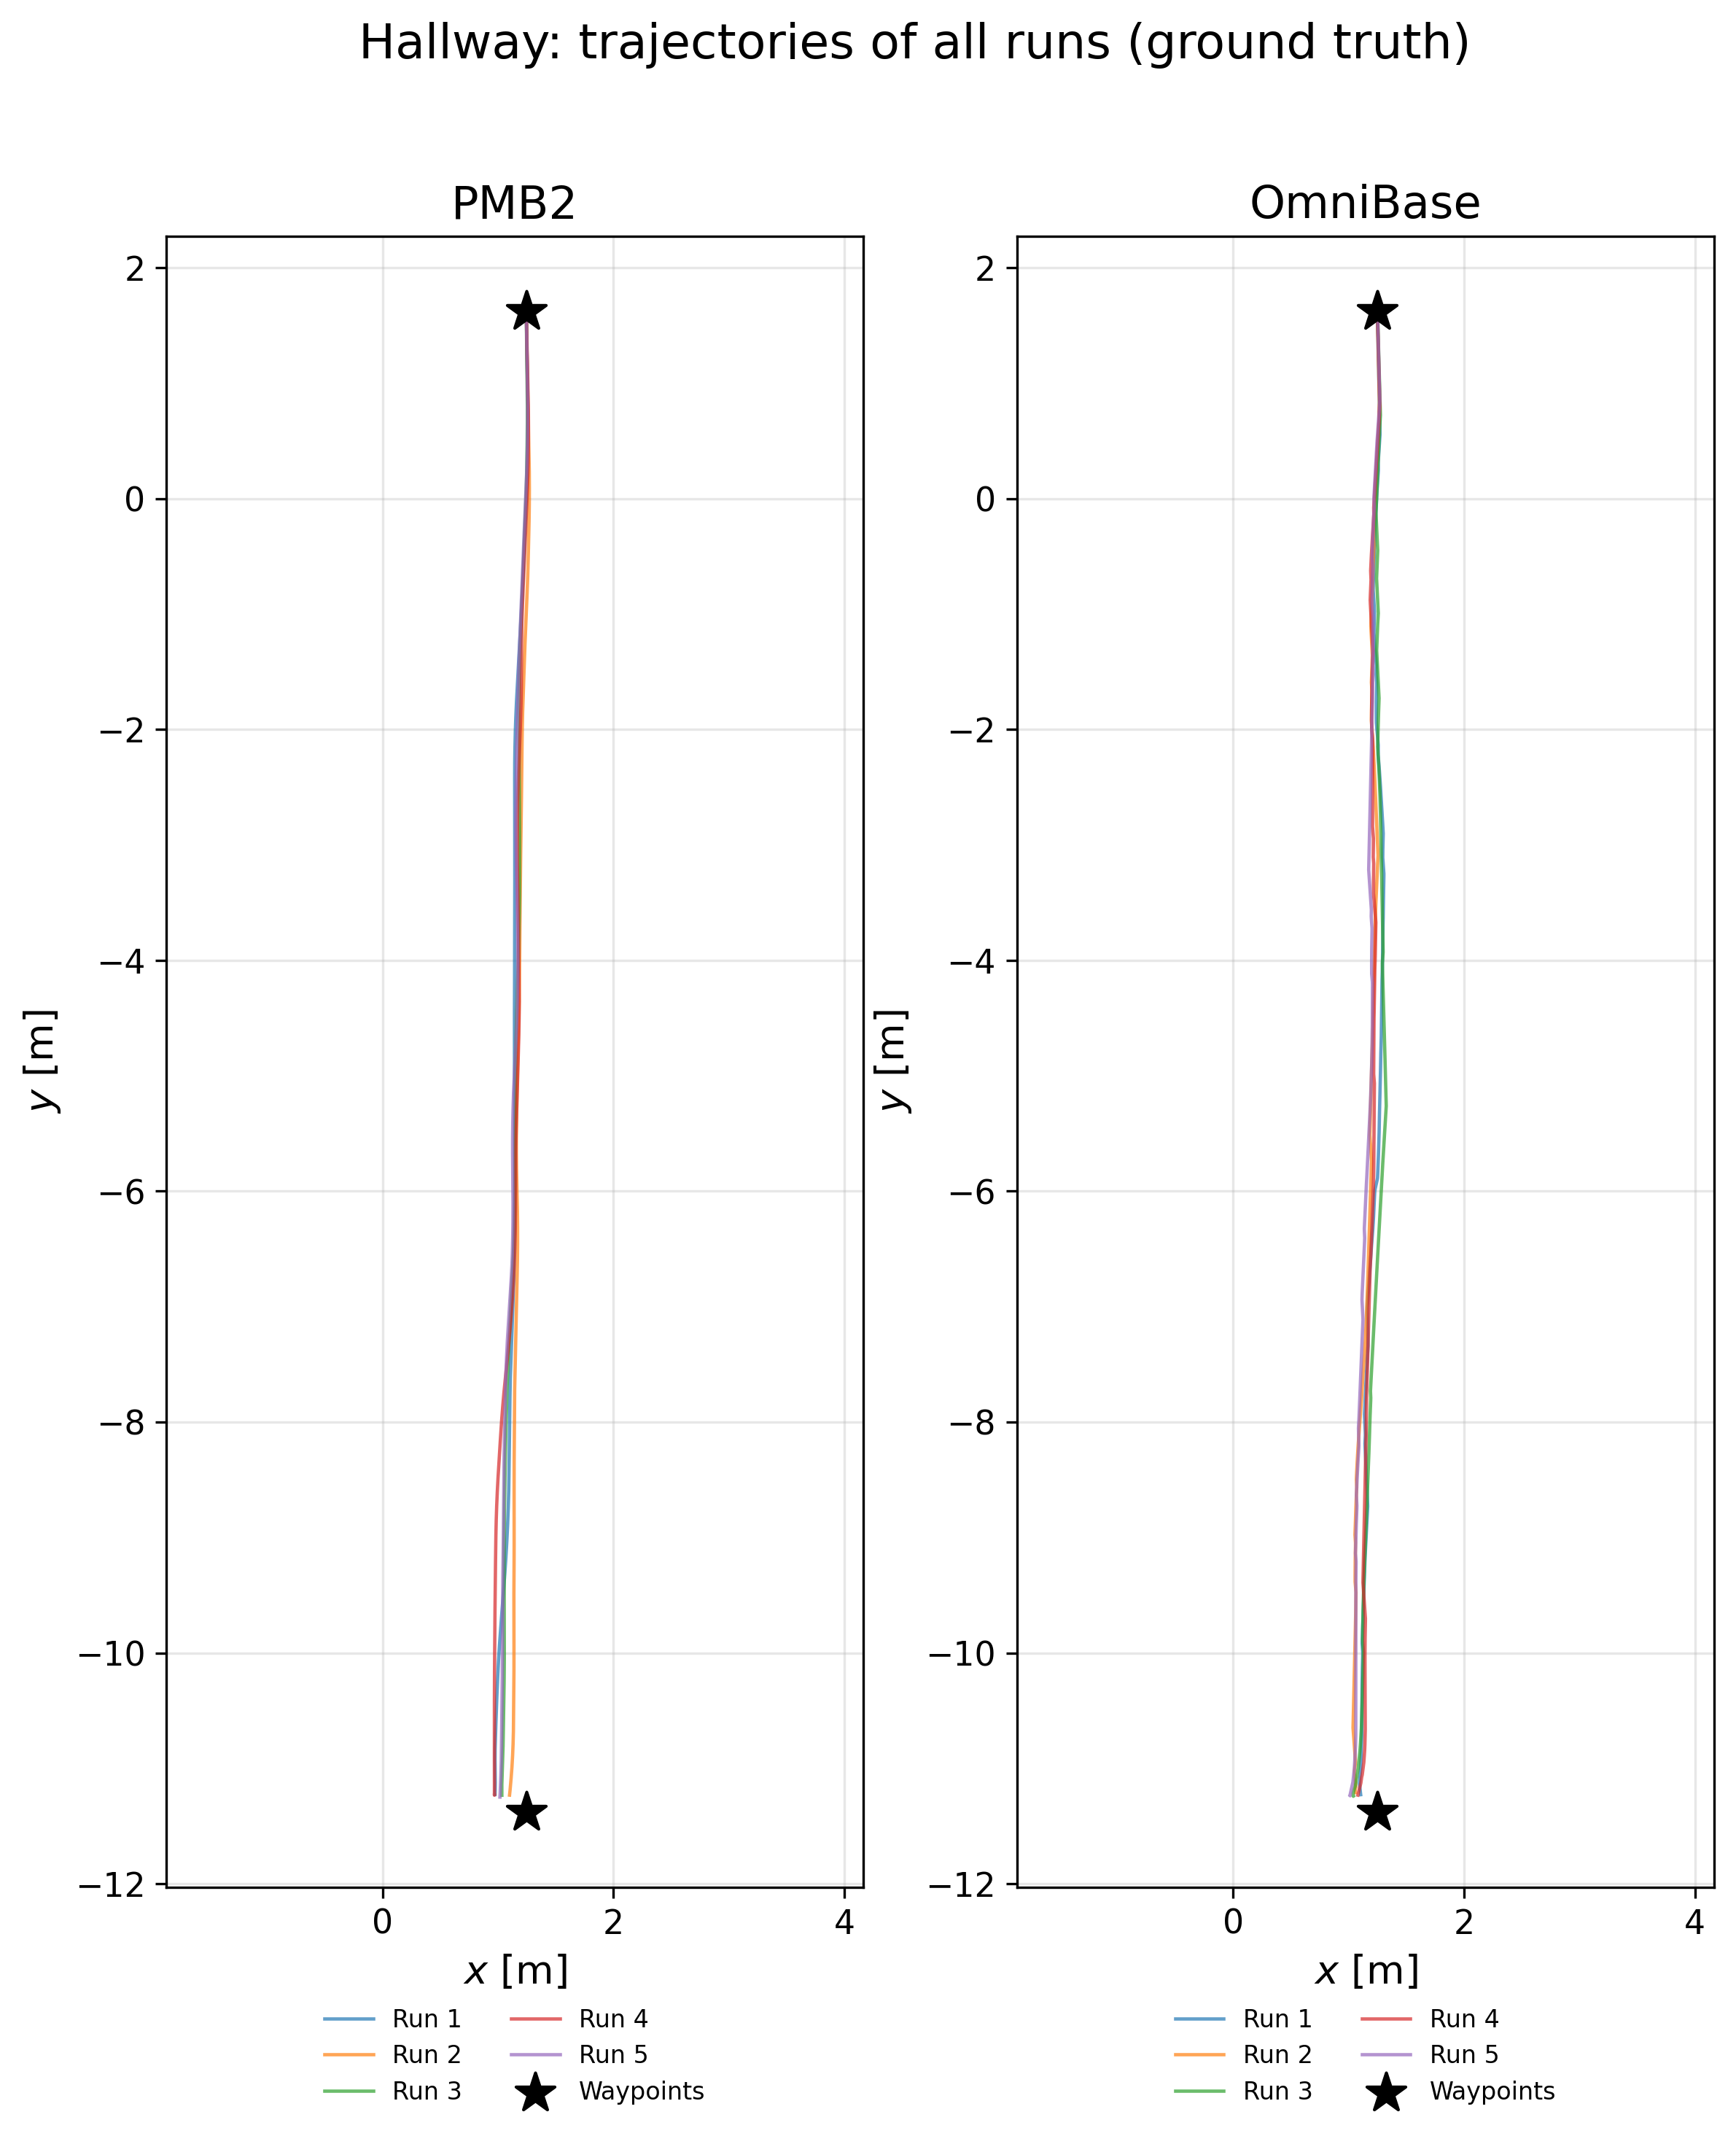
\includegraphics[width=1\textwidth]{images/Ch4/hallway/trajectories_all_Hallway.png}
  \caption{Straight corridor: Ground~Truth trajectories of all five runs per base. Both platforms follow the corridor axis with high repeatability. Stars mark the start (WP0) and the goal (WP1).}
  \label{fig:hallway-traj}
\end{figure}

Although both bases follow the corridor closely, the holonomic OmniBase tracks the planned path more faithfully. Its mean deviation from the Nav2 global plan is about a third smaller than the differential's ($0.079$ against $0.124$~m; RMS $0.100$ against $0.147$~m), and the same ordering holds for the maximum deviation. Figure~\ref{fig:hallway-xtrack} shows that for both platforms the deviation is negligible at the start and grows along the corridor, but the OmniBase keeps it consistently lower, its error curve repeatedly dipping as the base actively returns onto the planned path.

\begin{figure}[H]
  \centering
  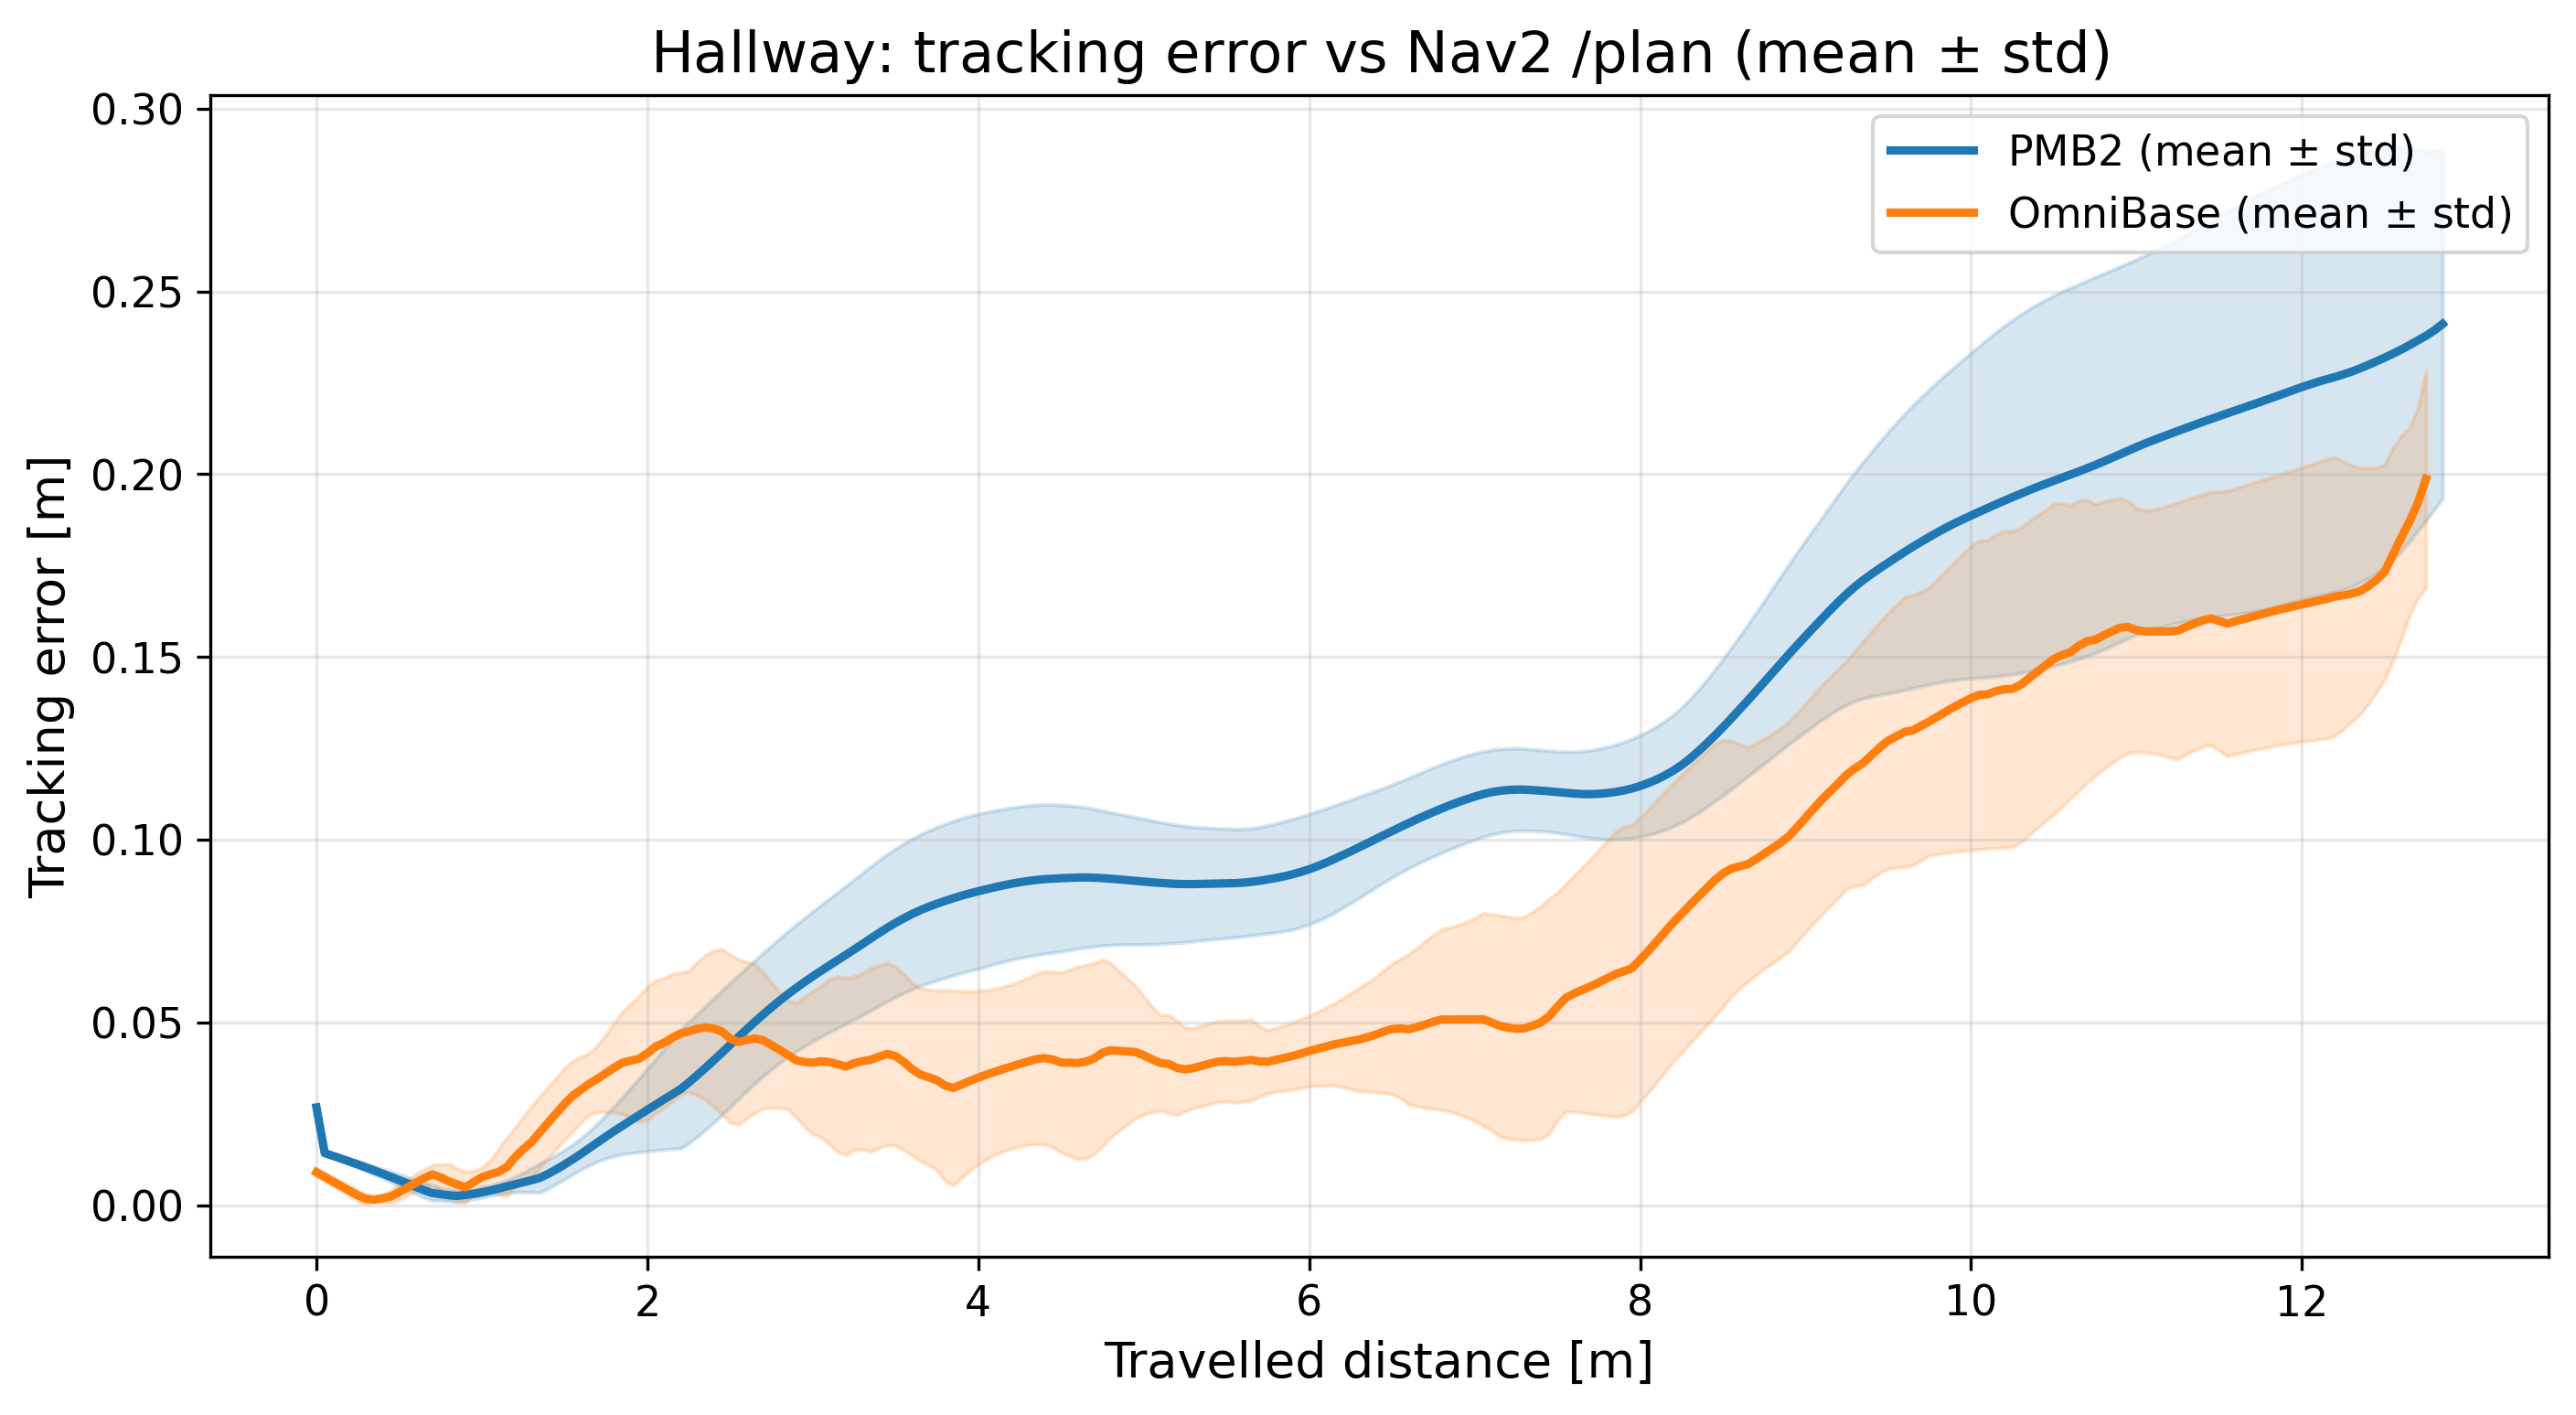
\includegraphics[width=1\textwidth]{images/Ch4/hallway/cross_track_band_Hallway.png}
  \caption{Straight corridor: tracking error against the Nav2 global plan as a function of travelled distance (mean $\pm$ standard deviation over five runs). The deviation grows along the corridor for both bases but remains consistently smaller for the holonomic OmniBase.}
  \label{fig:hallway-xtrack}
\end{figure}

This difference is explained by the commanded velocity profiles of Figure~\ref{fig:hallway-vel}. The OmniBase corrects lateral drift directly, through short pulses of lateral velocity $v_y$ (centre panel)---a capability reflected in a non-zero lateral usage ($0.075$) and structurally unavailable to the differential base, whose $v_y$ is identically zero and which can only realign by adjusting its heading through $\omega_z$. The two controllers, individually tuned, cruise at somewhat different peak forward speeds, yet cover the corridor in comparable time. The OmniBase also commands smoother linear motion (Table~\ref{tab:hallway}, \texttt{smooth\_lin} $0.845$ against $1.340$), a difference to be read in the light of the actuation-fidelity caveat of Section~\ref{subsec:m-fidelity}; the angular smoothness is instead essentially identical, since neither base turns appreciably on a straight path.

\begin{figure}[H]
  \centering
  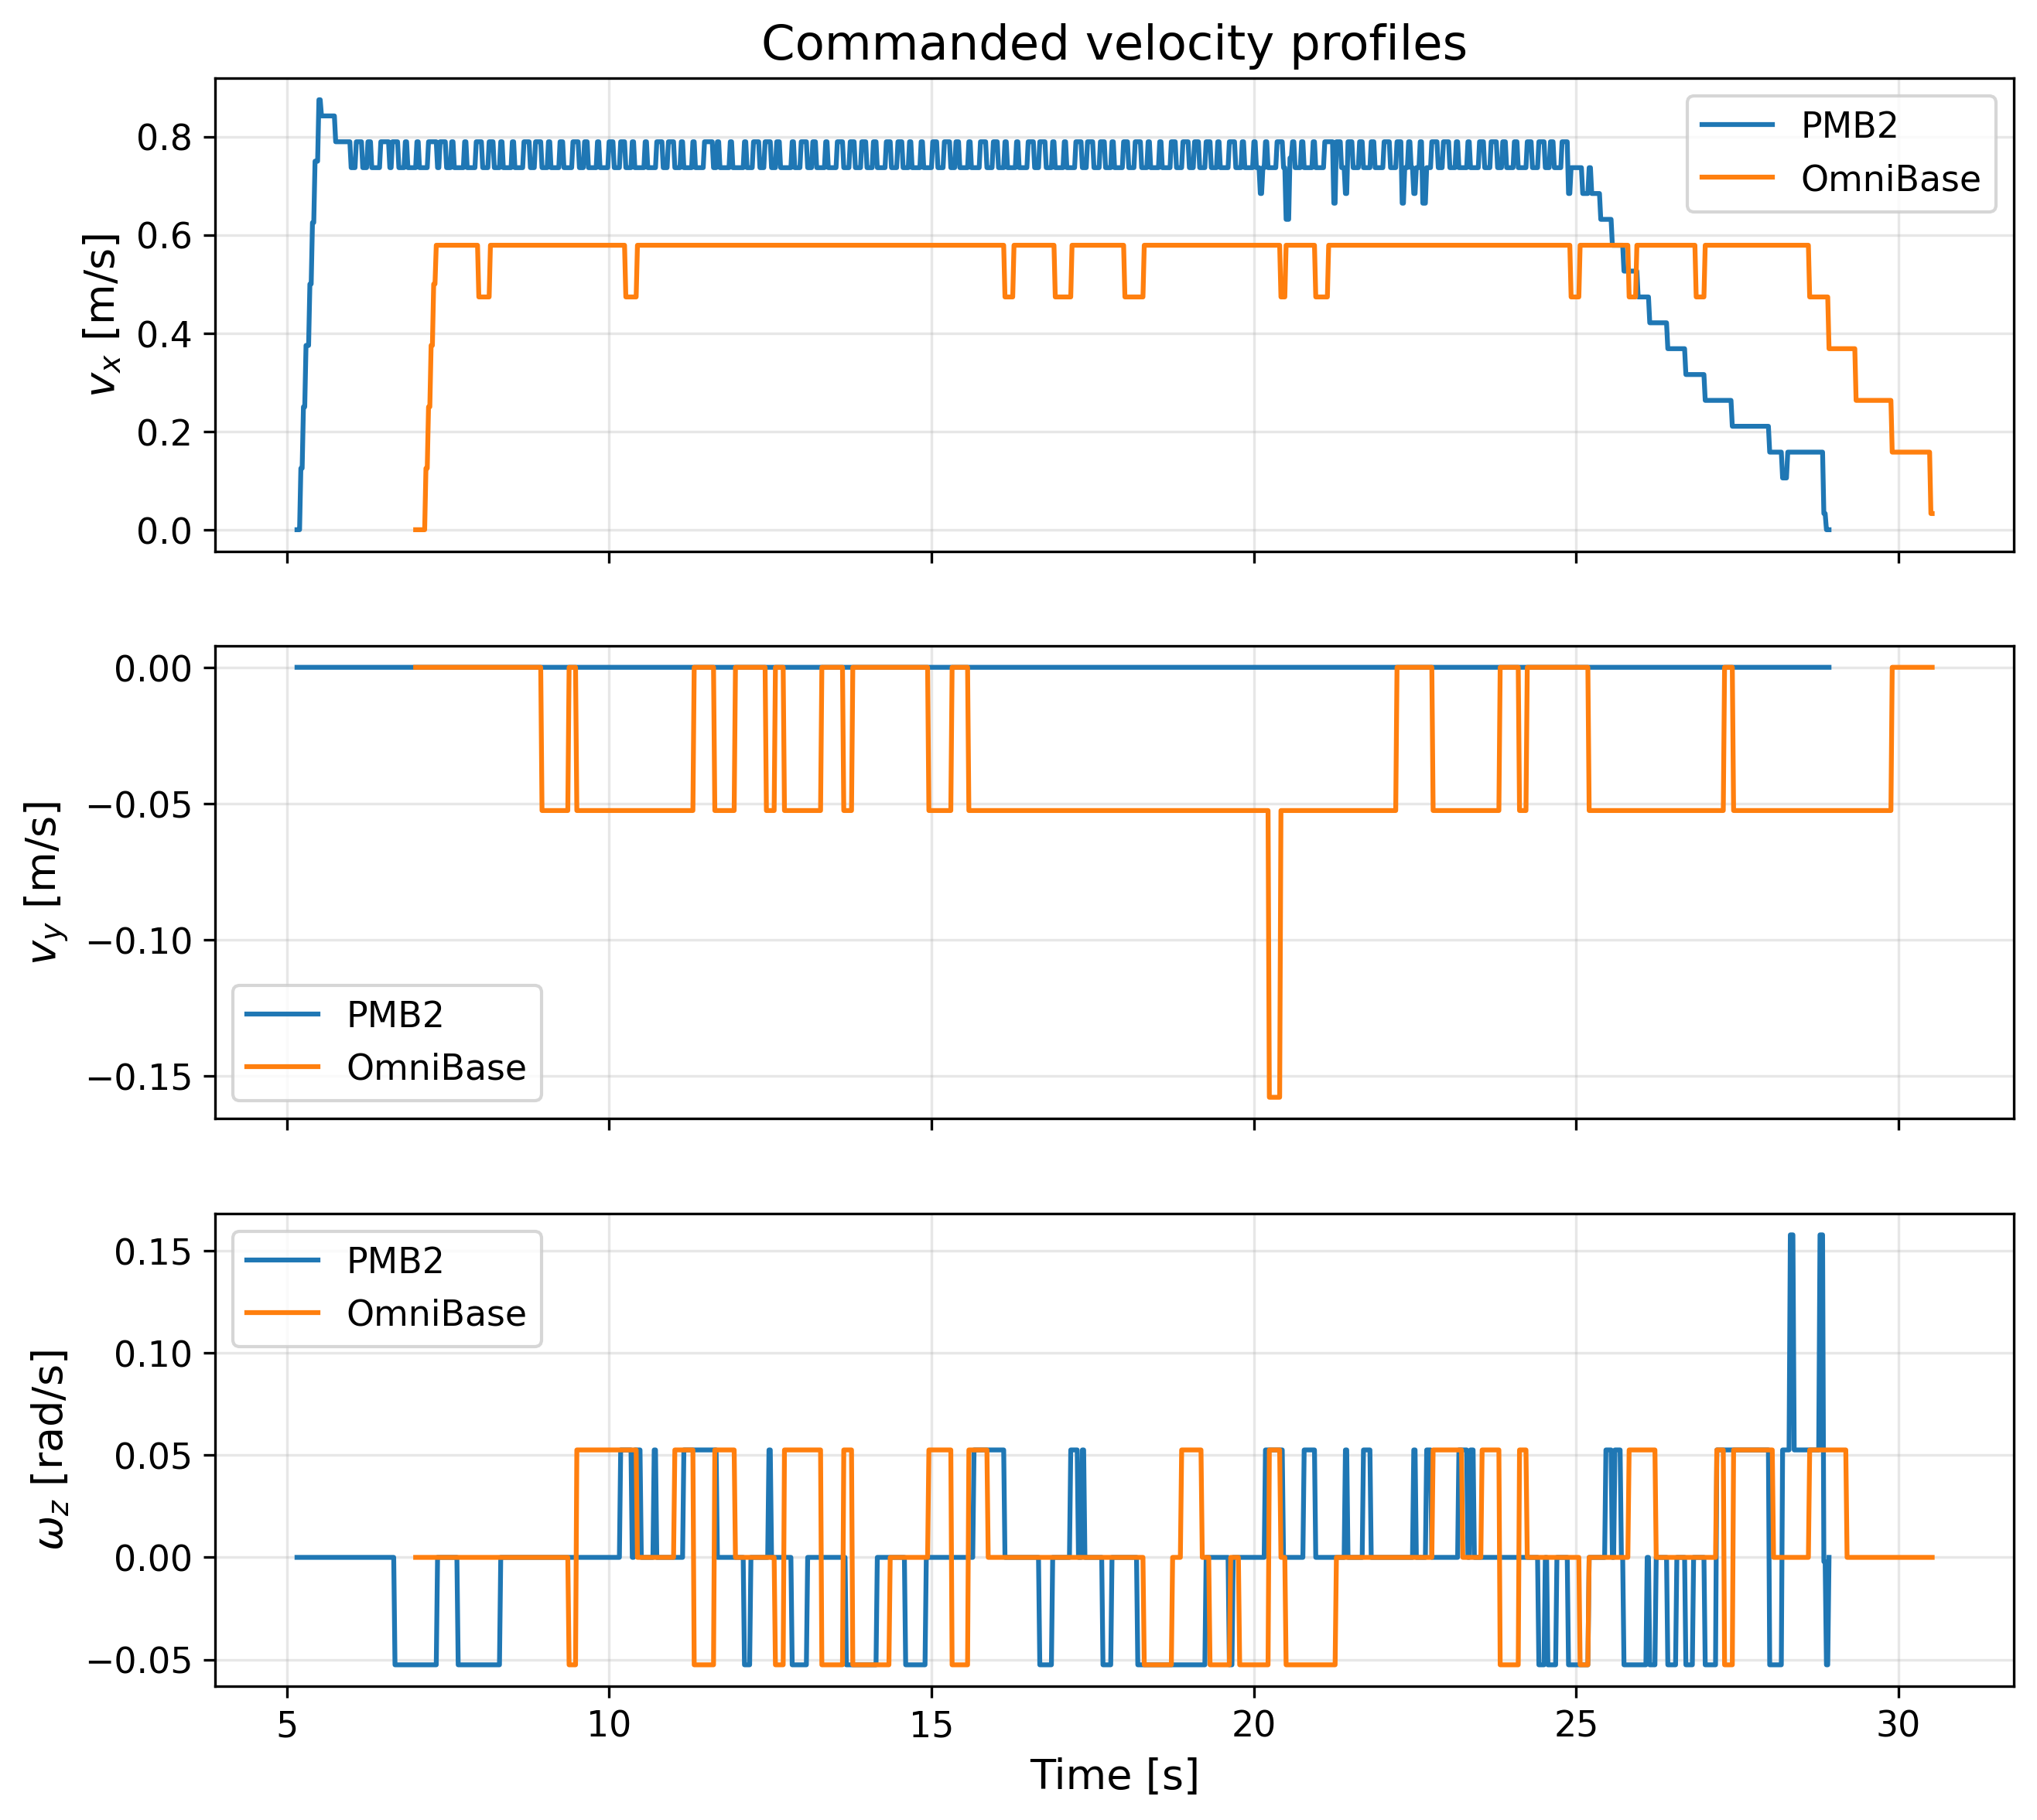
\includegraphics[width=1\textwidth]{images/Ch4/hallway/velocity_profiles.png}
  \caption{Straight corridor: commanded velocity profiles for the median run of each base. The OmniBase uses lateral velocity $v_y$ (centre) to correct drift, whereas the differential PMB2 keeps $v_y \equiv 0$ and relies on $\omega_z$ (bottom).}
  \label{fig:hallway-vel}
\end{figure}

The wheel-rotation profiles of Figures~\ref{fig:hallway-wheels-pmb2} and~\ref{fig:hallway-wheels-omni} complete the kinematic picture and connect these results to the models of Chapter~\ref{Ch:Kinematic}. For the differential PMB2, the left and right traction wheels rotate almost in unison and their position grows monotonically, the expected signature of straight-line motion with negligible steering; the accompanying velocity trace is obtained by differentiating the joint position, because the simulator returns an unreliable wheel-velocity field for this base. For the OmniBase, the four mecanum wheels cannot be read meaningfully from the simulator, since the \texttt{gazebo\_ros\_planar\_move} plugin imposes the body twist directly rather than actuating the wheels; the curves shown are therefore reconstructed by applying the inverse kinematic model of Chapter~\ref{Ch:Kinematic} to the commanded velocities, and depict the ideal, no-slip rotation that would realise the observed motion. They are included as an illustration of the wheel-level behaviour predicted by the kinematics, not as a measured signal.

\begin{figure}[htpb]
  \centering
  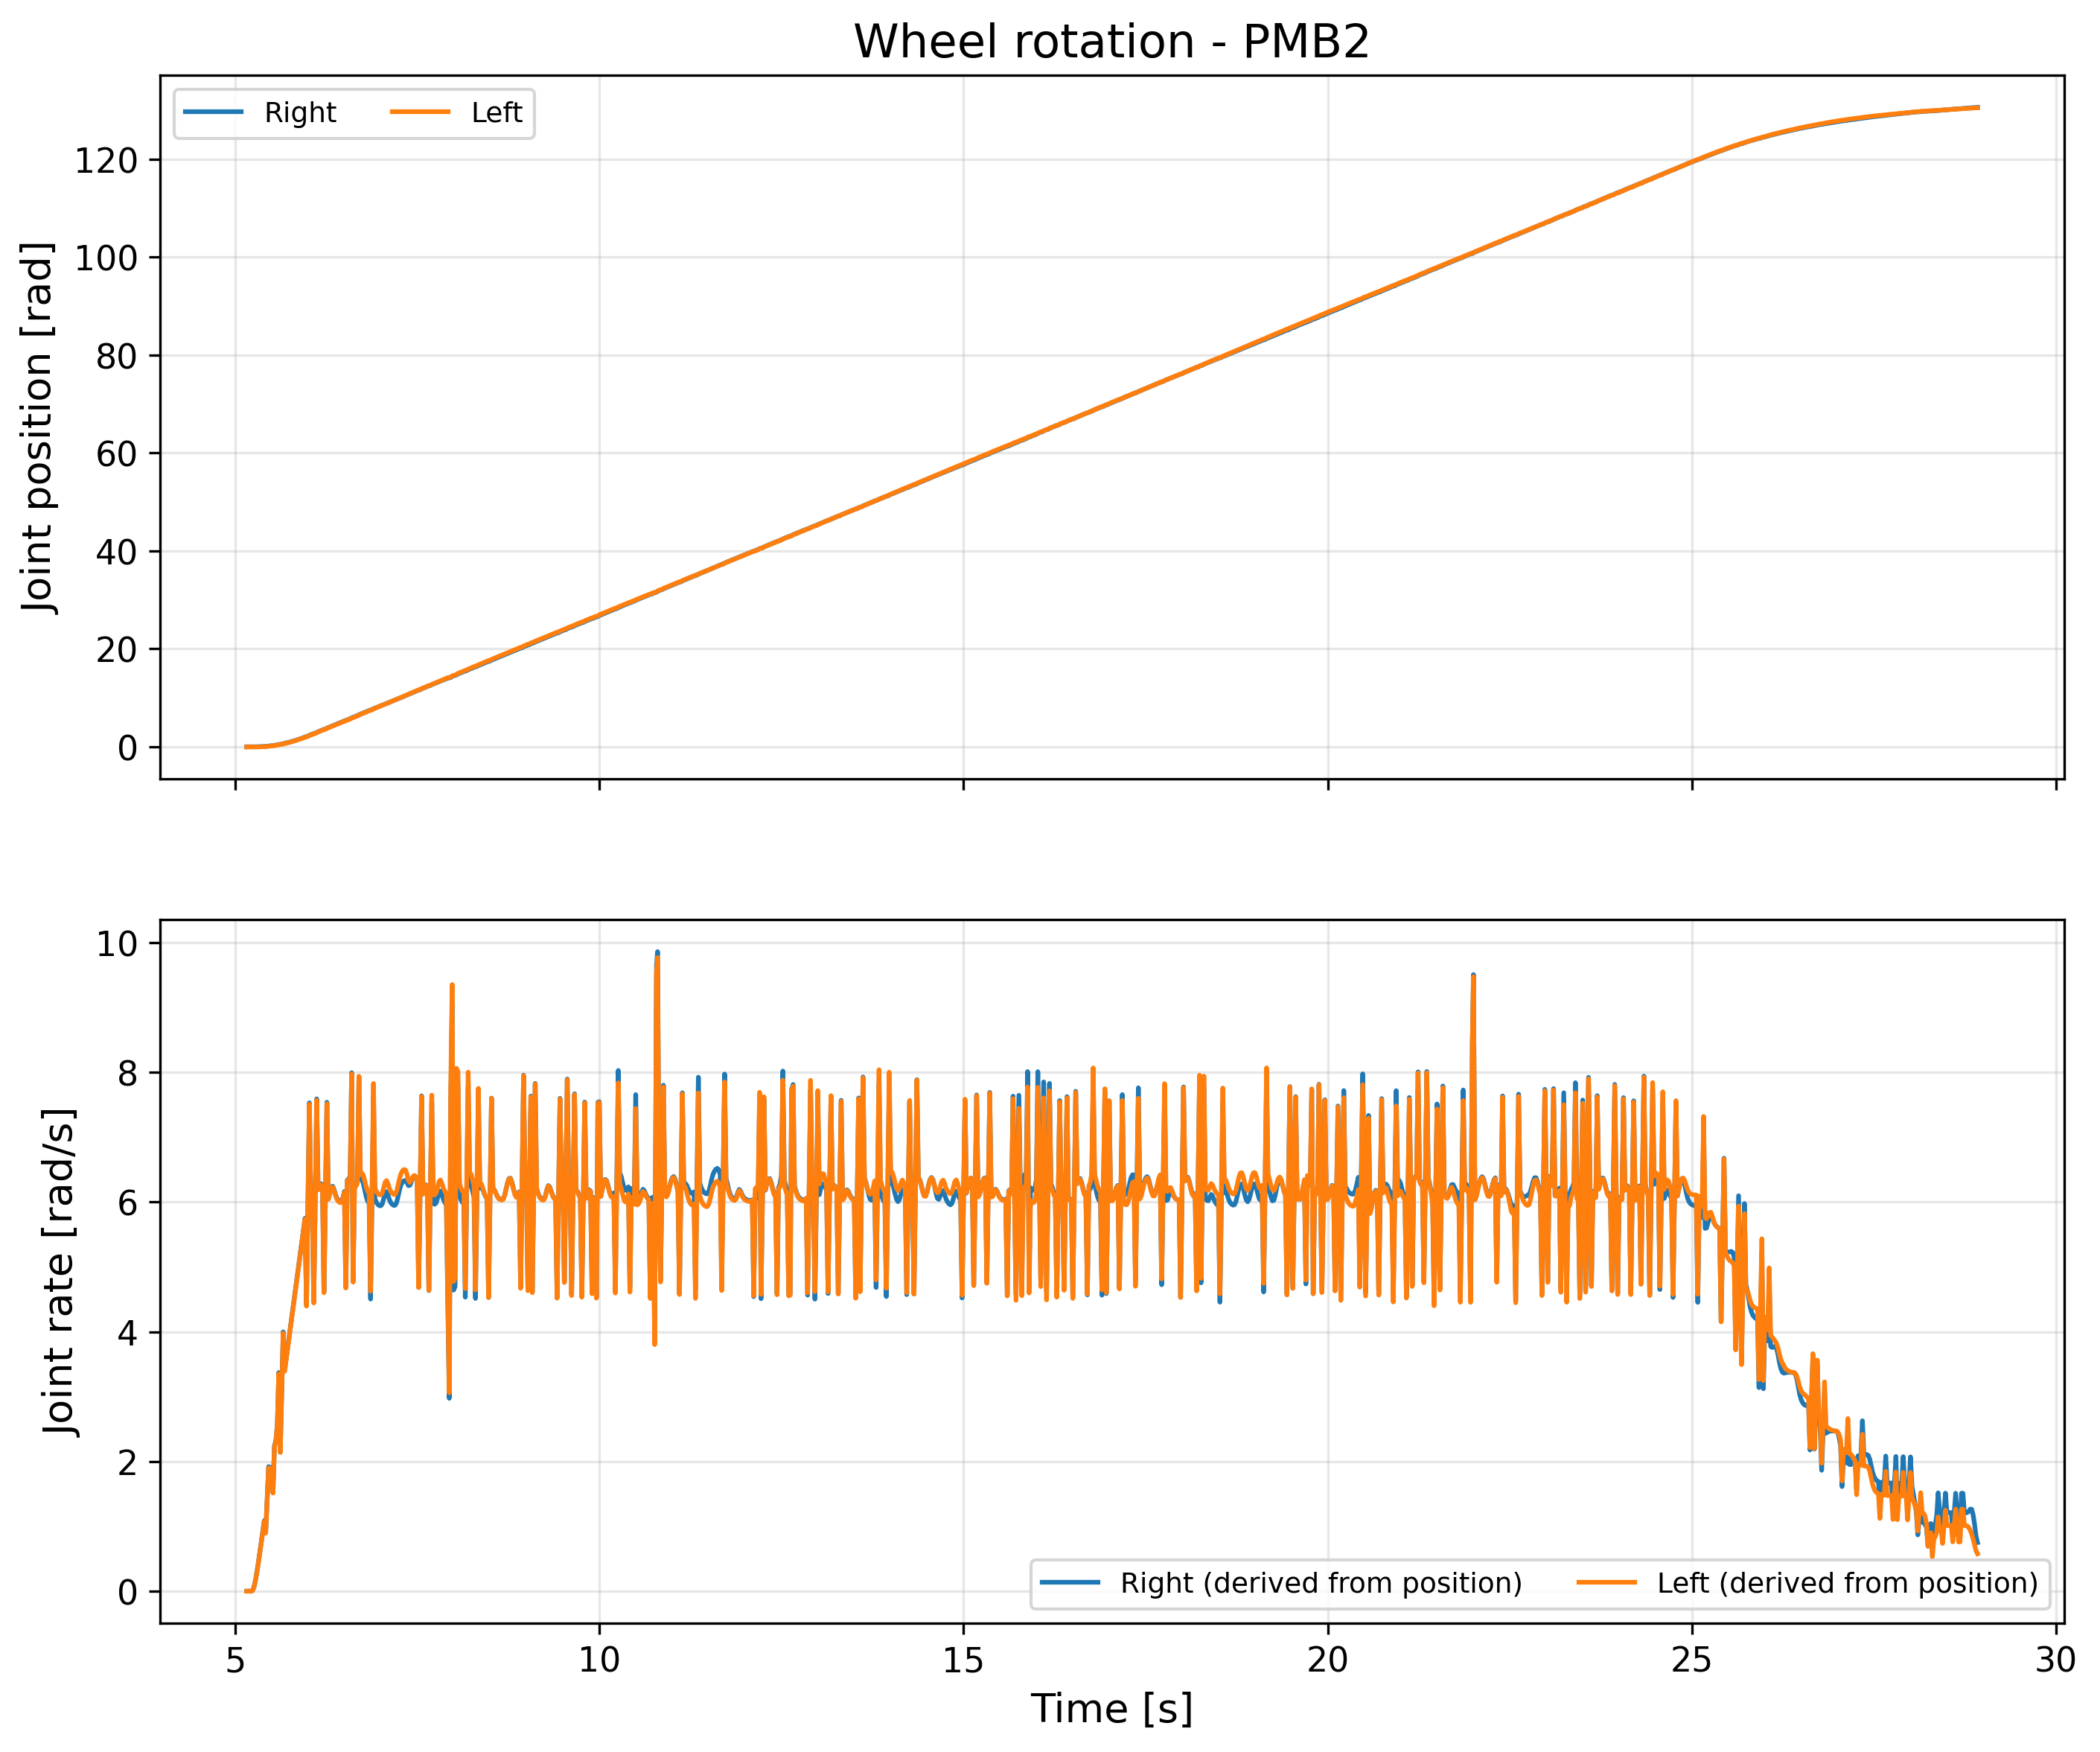
\includegraphics[width=1\textwidth]{images/Ch4/hallway/wheel_rotation_pmb2.png}
  \caption{Straight corridor: wheel rotation over time for the differential PMB2. The two traction wheels rotate almost identically, consistent with straight-line motion. The joint velocity (lower sub-panel) is derived numerically from the joint position, since the \texttt{velocity} field is unreliable in simulation; the resulting rotation is an ideal, no-slip one, which on a flat floor is effectively equivalent to the wheels' measured behaviour.}
  \label{fig:hallway-wheels-pmb2}
\end{figure}

\begin{figure}[htpb]
  \centering
  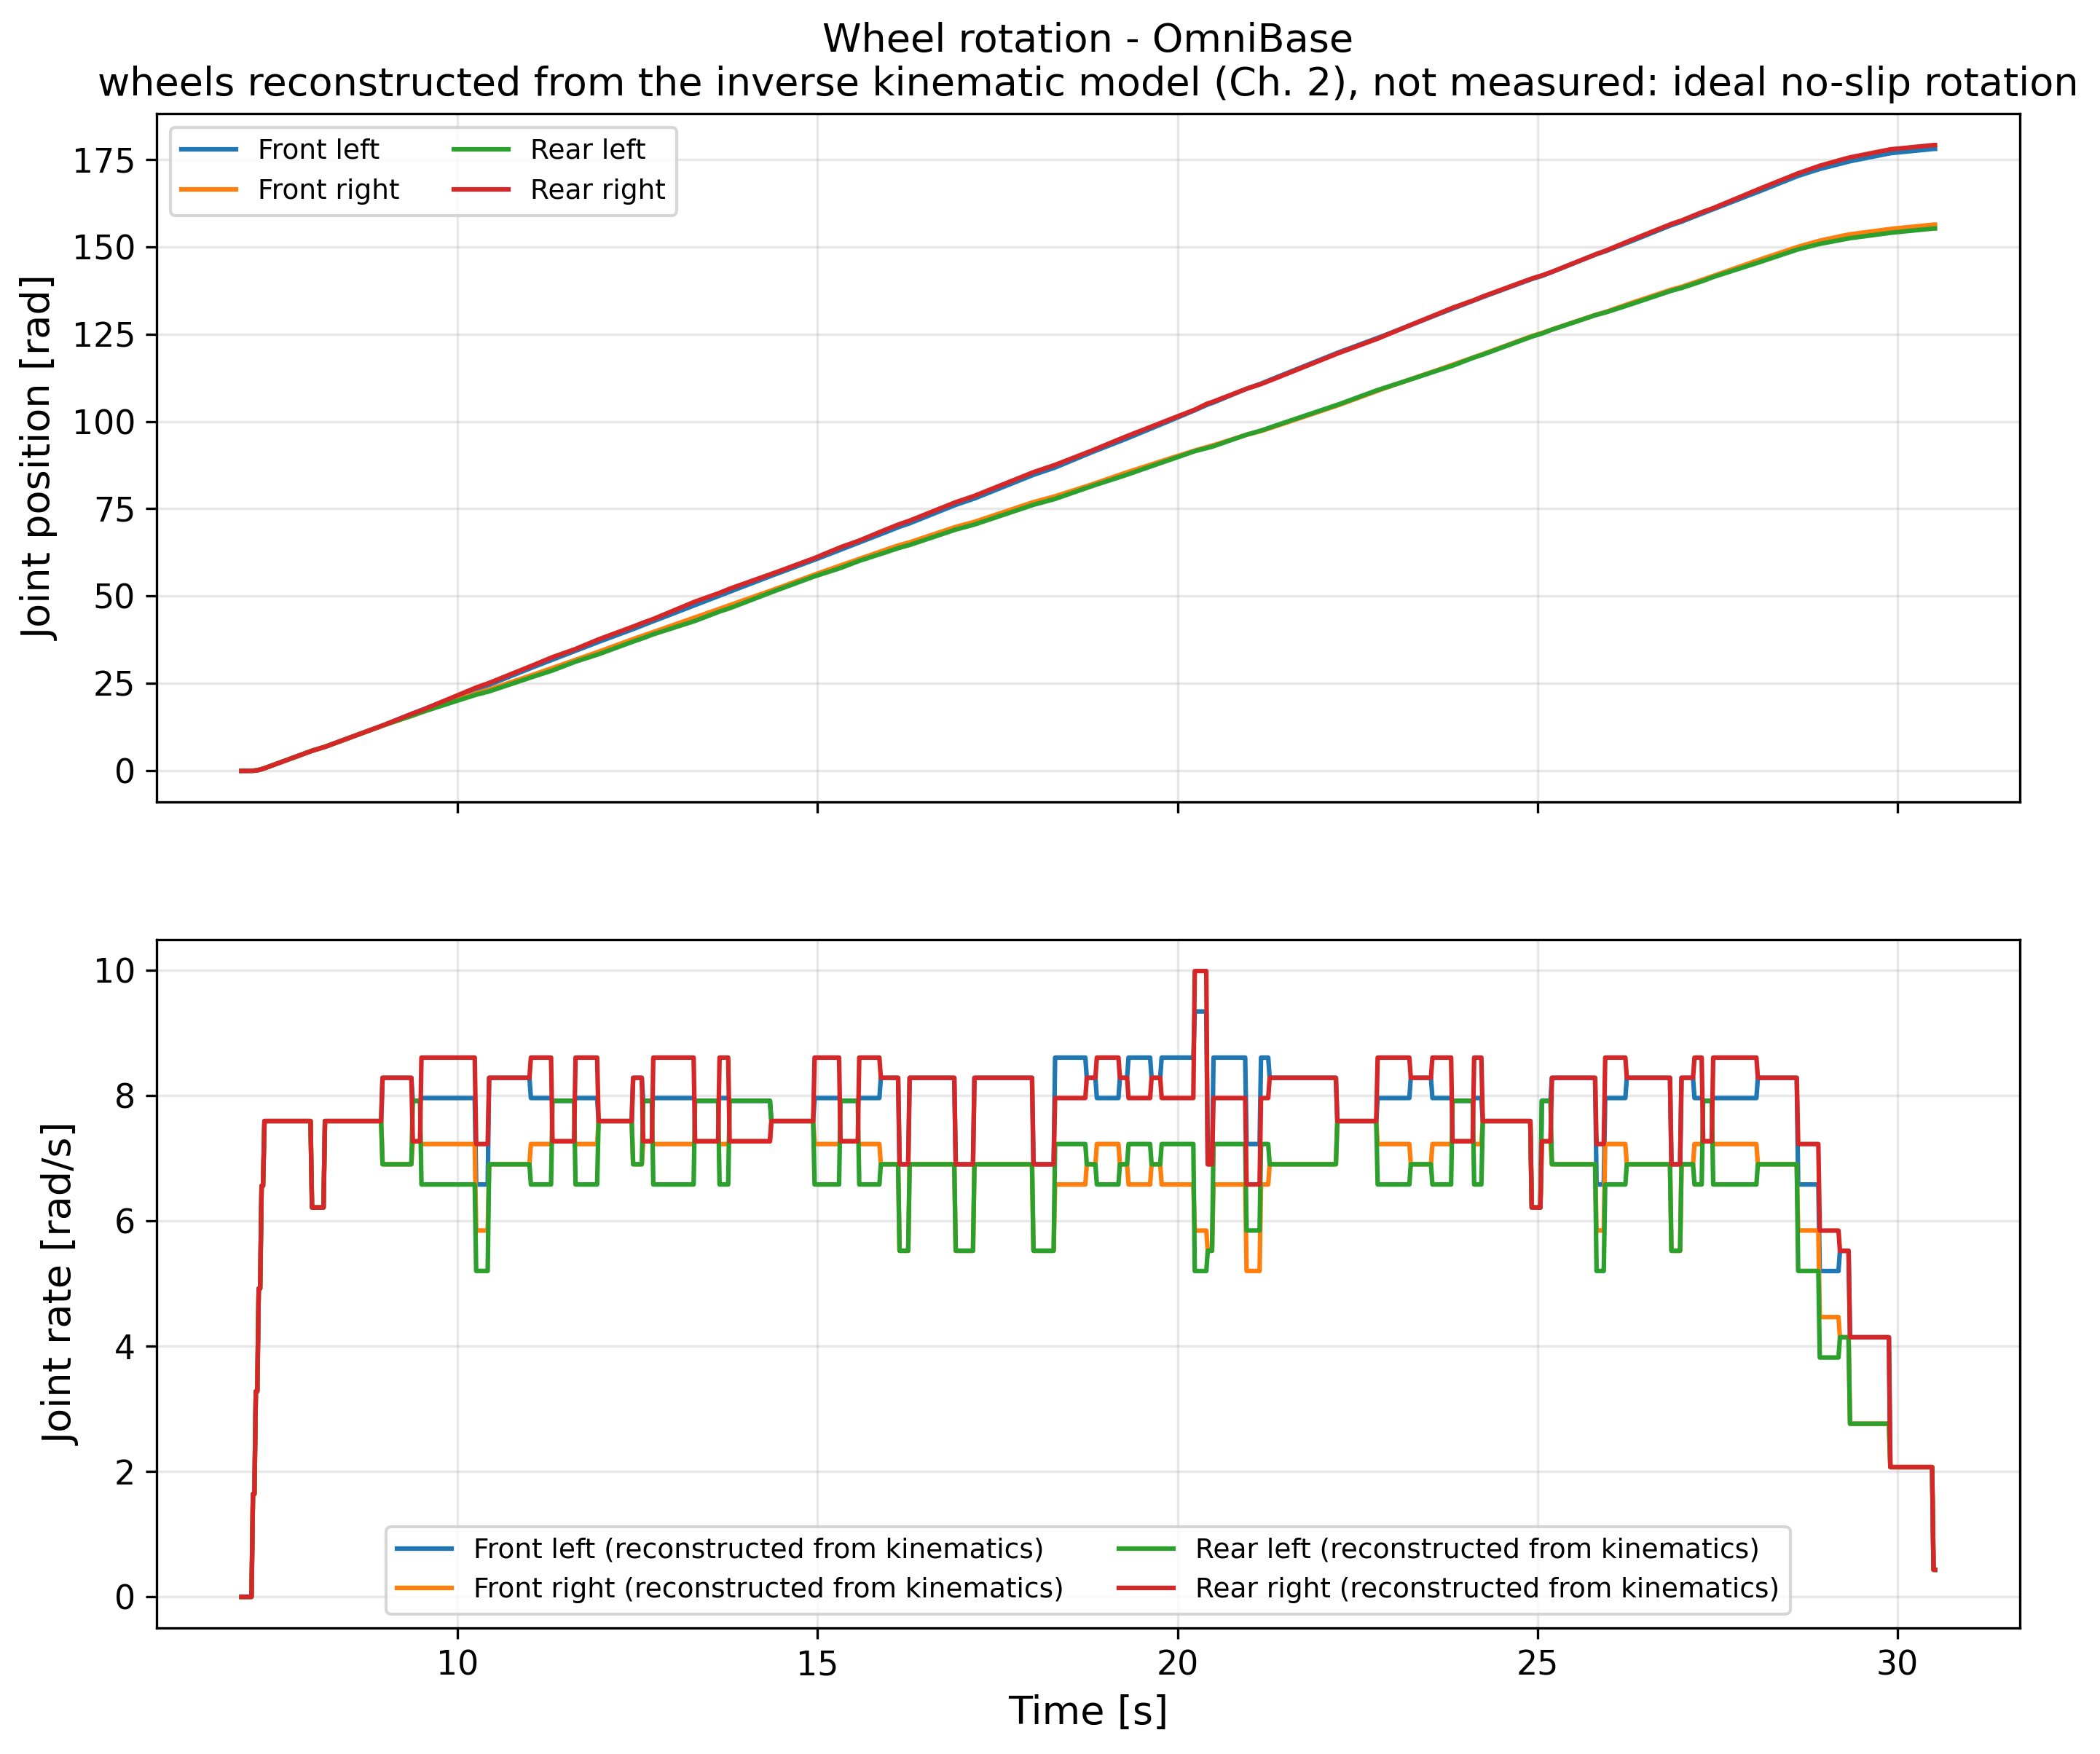
\includegraphics[width=1\textwidth]{images/Ch4/hallway/wheel_rotation_omni.png}
  \caption{Straight corridor: wheel rotation over time for the holonomic OmniBase. The four mecanum wheels are not read from the simulator---the \texttt{gazebo\_ros\_planar\_move} plugin imposes the body twist directly---but reconstructed by applying the inverse kinematic model of Chapter~\ref{Ch:Kinematic} to the commanded velocities, and therefore represent an ideal, no-slip rotation rather than a measured quantity. This shares the same idealised regime as the PMB2 wheel rotation of Figure~\ref{fig:hallway-wheels-pmb2}, which makes the two comparable at the kinematic level while remaining distinct from a comparison of actuation fidelity.}
  \label{fig:hallway-wheels-omni}
\end{figure}




At the goal the two platforms are comparably accurate, with a Ground~Truth positioning error of $0.238$~m for the OmniBase against $0.269$~m for the PMB2---both close to the $0.25$~m goal tolerance, the small excess reflecting the residual localisation offset at the stopping point. The OmniBase additionally shows a minor ($\approx 0.08$~m) offset already at the start waypoint, absent for the differential and attributable to a small initial-placement discrepancy, well within tolerance and without effect on task completion. In terms of efficiency the two bases are close, the OmniBase being marginally faster and markedly more repeatable ($23.56 \pm 0.14$~s against $24.10 \pm 0.52$~s), although part of this lower variance is itself a consequence of its idealised actuation (Section~\ref{subsec:m-fidelity}). Overall, on this trivial route holonomy translates into modestly tighter and smoother tracking, while the differential base remains fully competitive; the substantive differences between the two kinematics emerge only in the more demanding scenarios that follow.


\subsection{Sharp 90-Degree Corner (Path~B)}
\label{subsec:res-angle}

The sharp corner reverses the ranking observed on the straight corridor. Here the holonomic OmniBase is dramatically faster---it completes the route in $4.40 \pm 0.44$~s against $12.86 \pm 0.56$~s for the differential PMB2, almost a threefold difference---yet it tracks the planned path markedly \emph{worse}, its mean deviation from the Nav2 plan being about four times larger ($0.233$ against $0.055$~m). Both platforms again reached the goal in every run without planning failures; the only recovery recorded across the two simple routes was a single costmap-clearing action in one PMB2 run. The aggregate metrics are reported in Table~\ref{tab:angle}, and the two navigation strategies are contrasted in Figure~\ref{fig:angle-traj}.

\begin{table}[htbp]
\centering
\caption{Sharp corner (Path~B): aggregate metrics, mean $\pm$ standard deviation over five runs.}
\label{tab:angle}
\begin{tabular}{lcc}
\toprule
Metric & PMB2 (differential) & OmniBase (holonomic) \\
\midrule
Completion time [s]              & $12.86 \pm 0.56$ & $4.40 \pm 0.44$ \\
Average speed [m/s]              & $0.155 \pm 0.006$ & $0.429 \pm 0.040$ \\
Tracking error, mean [m]        & $0.055 \pm 0.012$ & $0.233 \pm 0.011$ \\
Tracking error, RMS [m]         & $0.104 \pm 0.004$ & $0.287 \pm 0.009$ \\
Mean waypoint error [m]         & $0.230 \pm 0.004$ & $0.316 \pm 0.016$ \\
Corner (WP1) waypoint error [m] & $0.590 \pm 0.004$ & $0.776 \pm 0.019$ \\
Mean orientation error [rad]    & $0.661 \pm 0.014$ & $0.048 \pm 0.022$ \\
Linear smoothness [m/s$^2$]     & $1.174 \pm 0.099$ & $1.827 \pm 0.117$ \\
Angular smoothness [rad/s$^2$]  & $1.849 \pm 0.191$ & $1.014 \pm 0.127$ \\
Lateral usage                    & $0.000 \pm 0.000$ & $0.669 \pm 0.016$ \\
\bottomrule
\end{tabular}
\end{table}

\begin{figure}[H]
  \centering
  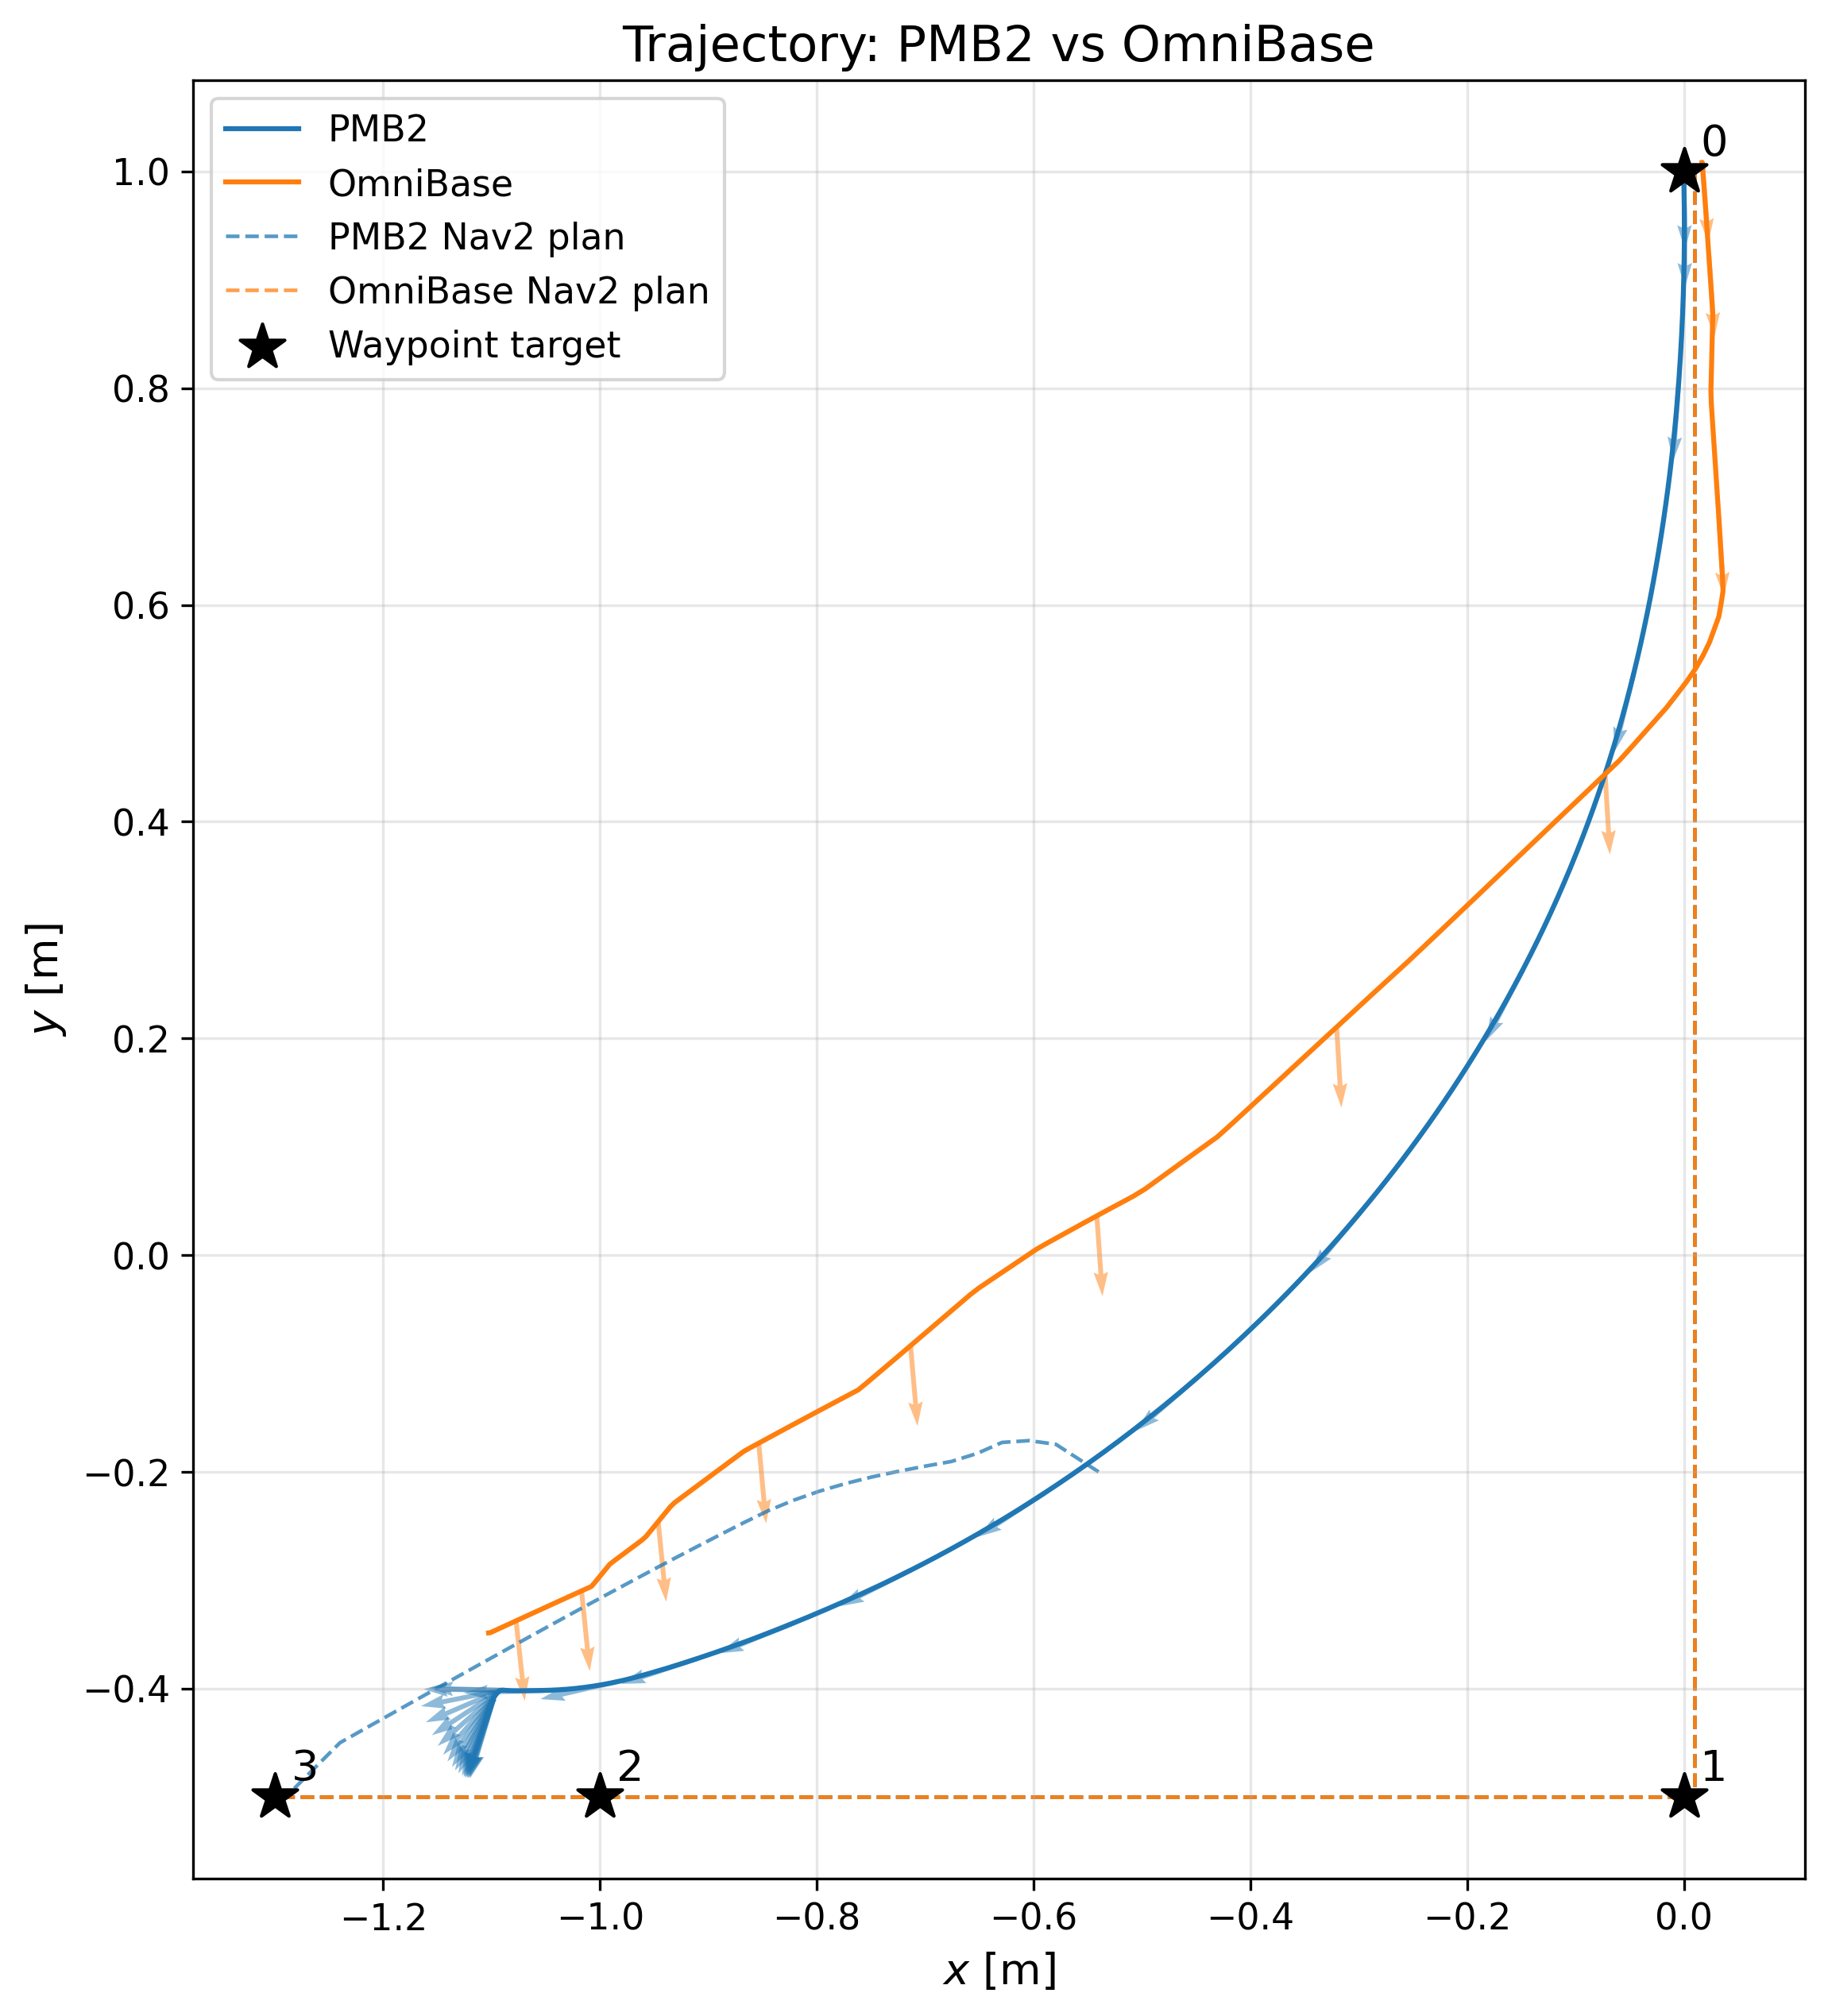
\includegraphics[width=1\textwidth]{images/Ch4/angle/trajectory_comparison.png}
  \caption{Sharp corner: Ground~Truth trajectory of the median run of each base, with the corresponding Nav2 global plans (dashed) and heading arrows. Neither base reaches the corner waypoint (WP1): both round it. The OmniBase keeps a fixed south-facing heading while strafing along a diagonal shortcut, whereas the PMB2 rotates to follow the path tangent and performs a final in-place rotation near the goal.}
  \label{fig:angle-traj}
\end{figure}

Because \texttt{NavigateThroughPoses} does not stop at the intermediate poses, both platforms cut the corner heavily: neither approaches the corner waypoint (WP1) closer than about $0.6$~m (PMB2) or $0.8$~m (OmniBase), and this closest-approach distance---following the definition of Section~\ref{subsec:m-accuracy}---is precisely the extent of the corner-cutting rather than a positioning failure. The manner of the cut, however, differs fundamentally. The OmniBase exploits its lateral degree of freedom (lateral usage $0.669$) to translate diagonally towards the second leg while holding an almost constant heading, tracing a single straight shortcut. The PMB2, unable to strafe, negotiates the turn as a smooth curve, continuously rotating so that its heading follows the direction of travel, as the arrows in Figure~\ref{fig:angle-traj} show.

\begin{figure}[H]
  \centering
  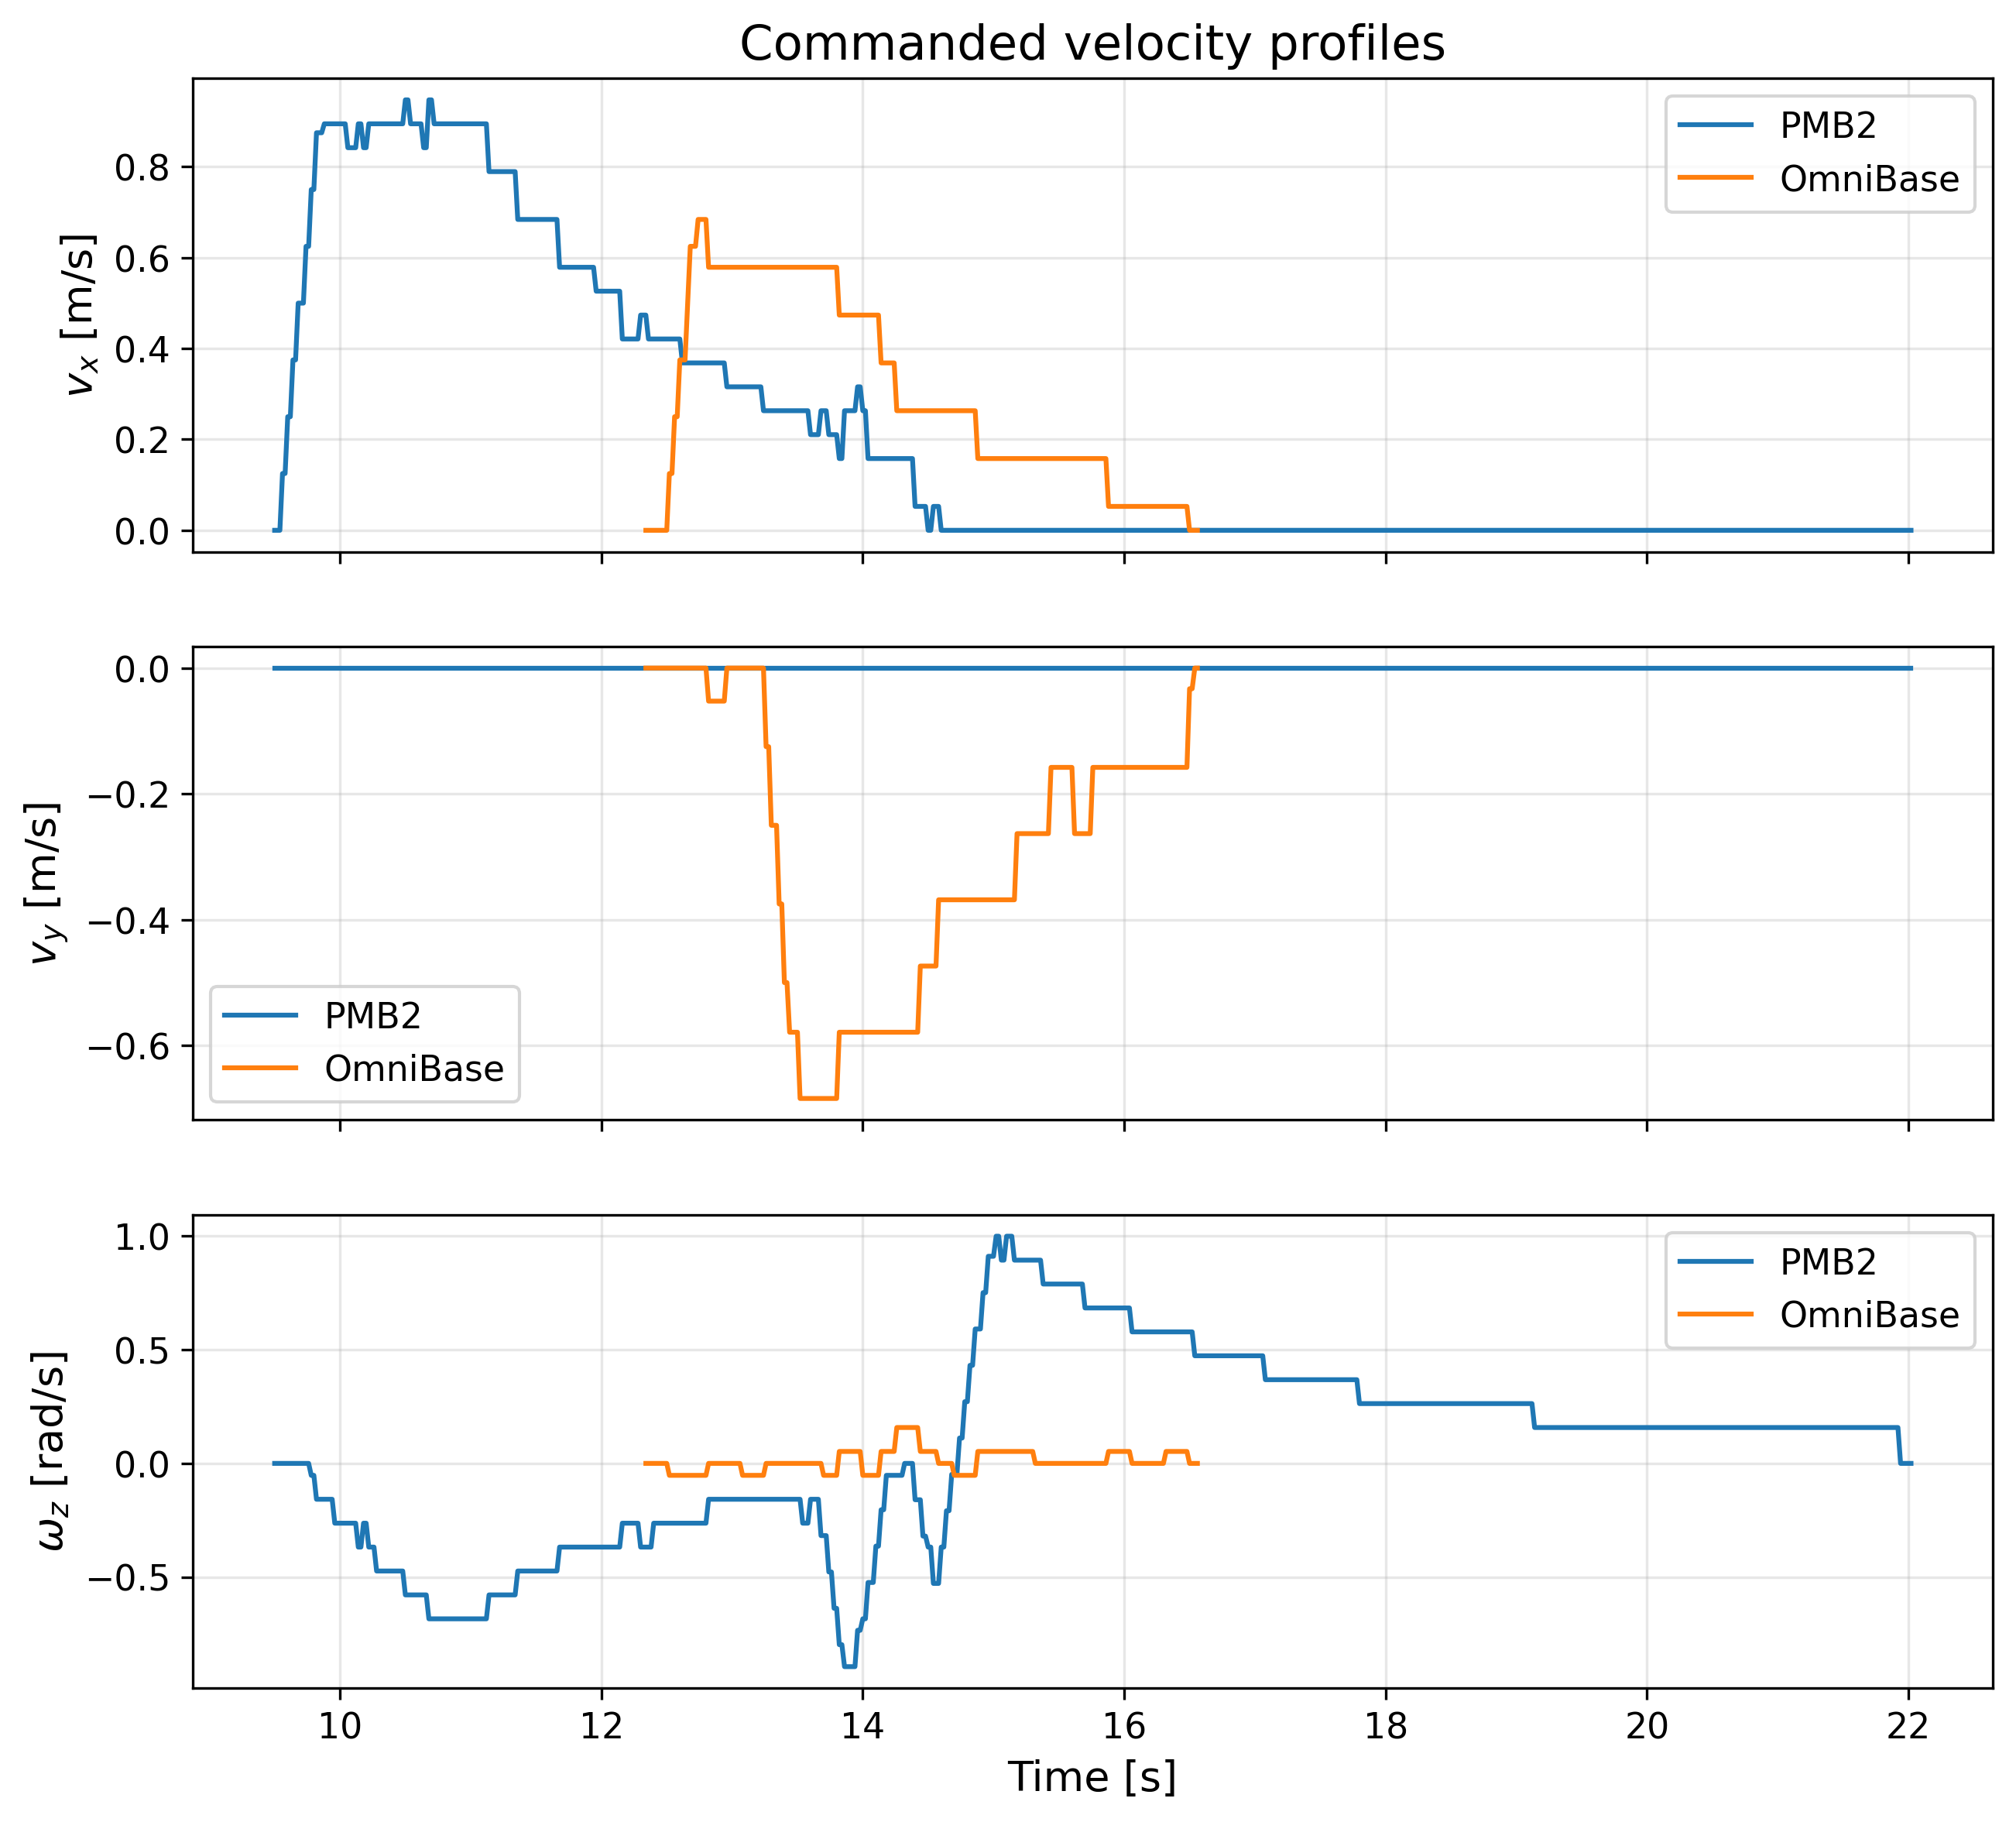
\includegraphics[width=1\textwidth]{images/Ch4/angle/velocity_profiles.png}
  \caption{Sharp corner: commanded velocity profiles for the median run of each base. The OmniBase performs the turn through a pulse of lateral velocity $v_y$ (centre) with $\omega_z \approx 0$, while the PMB2 keeps $v_y \equiv 0$ and turns through $\omega_z$, including a pronounced terminal burst (bottom) corresponding to the final in-place rotation.}
  \label{fig:angle-vel}
\end{figure}

The velocity profiles of Figure~\ref{fig:angle-vel} make the two mechanisms explicit and explain the large time gap. The OmniBase realises the entire manoeuvre with a single burst of lateral velocity (peaking near $-0.7$~m/s) while keeping $\omega_z$ close to zero; it never rotates, and finishes quickly. The PMB2 instead turns entirely through $\omega_z$, and---crucially---arrives at the goal travelling westwards while the commanded final orientation points south, so it must perform a final in-place rotation to satisfy the goal-orientation tolerance. This terminal rotation, visible as the pronounced $\omega_z$ burst and the long low-speed tail at the end of the differential's profile, accounts for a large part of the threefold difference in completion time and for the differential's higher angular acceleration ($1.849$ against $1.014$~rad/s$^2$). The trade-off is mirrored in the linear smoothness, where the ordering is now the opposite of the corridor: the OmniBase is linearly \emph{rougher} ($1.827$ against $1.174$~m/s$^2$), the transient of its sharp strafe outweighing the differential's gentler forward profile.

\begin{figure}[H]
  \centering
  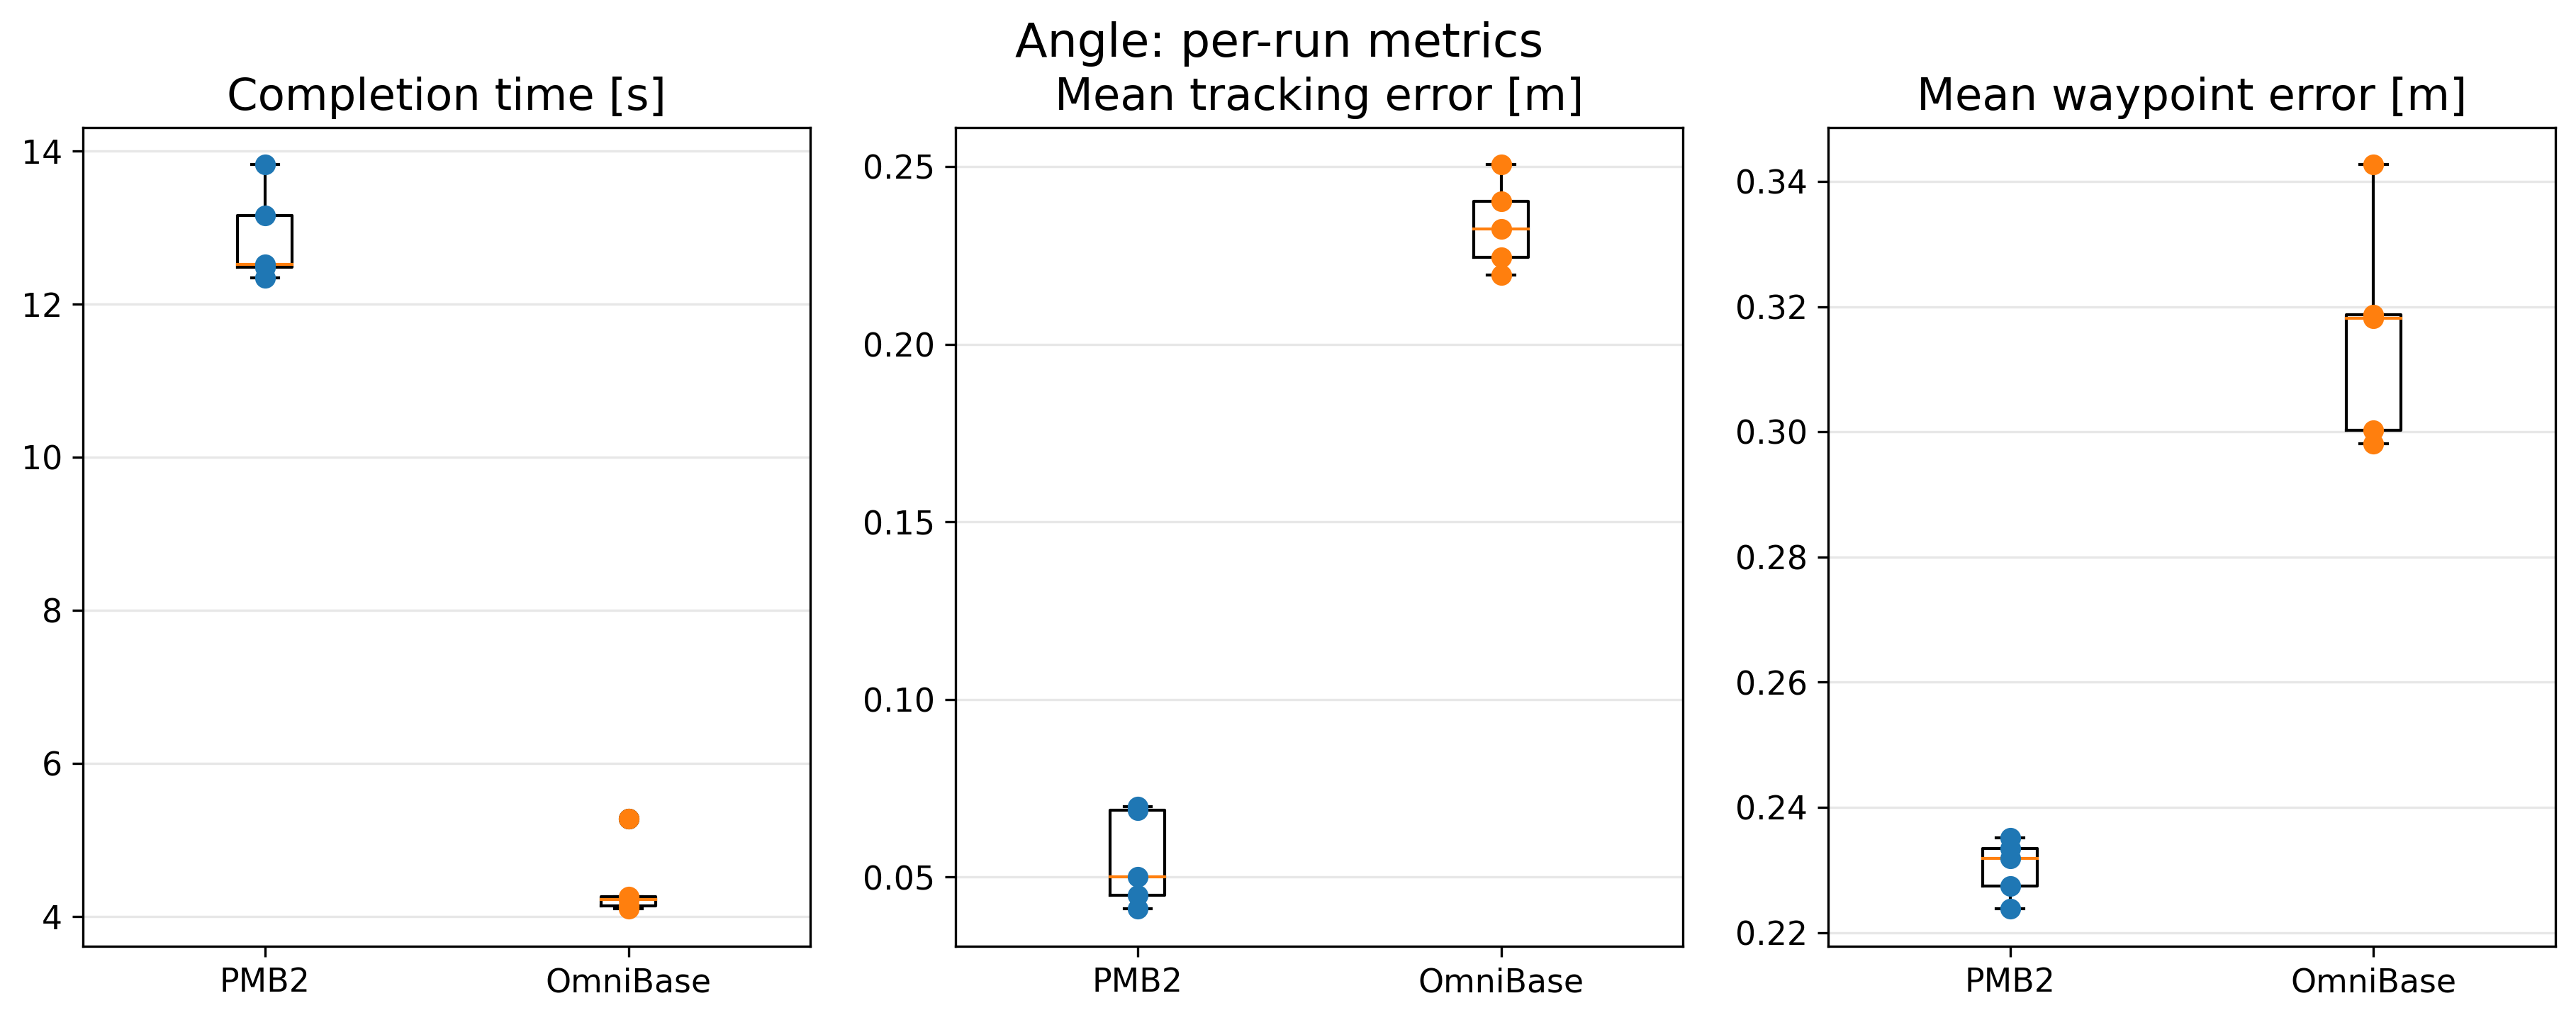
\includegraphics[width=1\textwidth]{images/Ch4/angle/boxplots_Angle.png}
  \caption{Sharp corner: per-run distribution of completion time, mean tracking error, and mean waypoint error. The OmniBase is consistently far faster but exhibits systematically larger tracking and waypoint errors.}
  \label{fig:angle-box}
\end{figure}

The per-run distributions in Figure~\ref{fig:angle-box} confirm that these differences are systematic across repetitions rather than isolated to a single run. The tracking-error reversal deserves emphasis: whereas on the straight corridor holonomy produced tighter path-following, on the corner it is the differential that adheres more closely to the plan. The reason is that the holonomic shortcut, being a single diagonal, departs from the L-shaped global plan over a longer stretch, while the differential follows a curve that hugs the plan more closely and, once past the corner, quickly settles back onto the second leg. Finally, the orientation-error figures ($0.661$~rad for the PMB2 against $0.048$~rad for the OmniBase) must be read through the caveat of Section~\ref{subsec:m-accuracy}: the intermediate waypoint headings are decorative and were all specified towards south, coinciding with the heading the OmniBase happens to maintain while strafing, so its small value reflects heading stability rather than active orientation control; the differential's large value likewise reflects its constantly changing heading along the curve, not a failure to reach a commanded pose. In summary, on a sharp corner holonomy converts into a decisive speed advantage through lateral motion, at the cost of looser adherence to the planned path, whereas the differential drive stays closer to the plan but pays for the required rotations in time and angular effort---the absolute smoothness and variance values remaining subject to the actuation-fidelity caveat of Section~\ref{subsec:m-fidelity}.

\subsection{Cluttered Obstacle Course (Path~C)}
\label{subsec:res-obstacles}

The cluttered obstacle course is the route that most directly probes navigation robustness, and it exposes the sharpest qualitative difference of the whole waypoint campaign. Both platforms completed all five runs and traced the full winding circuit through the eleven waypoints. The decisive difference lies not in whether the goal is reached, but in how much the planning stack struggles to reach it: the differential PMB2 incurred at least one planning failure in \emph{every} run (between one and five, about $4\%$ of its planning attempts), whereas the holonomic OmniBase never failed to plan in any run. The aggregate metrics are reported in Table~\ref{tab:obs}.

Figure~\ref{fig:obs-traj} shows the Ground~Truth trajectories of all five runs of each base. Both platforms trace the full winding circuit through the eleven waypoints, and the geometry of the two sets of paths is essentially the same: the kinematic difference does not alter the route taken, only the way it is executed. The two bases differ, however, in run-to-run consistency. The OmniBase trajectories are almost perfectly superimposed along the entire circuit, whereas the PMB2 ones visibly fan out at a few points---most noticeably along the stretches approaching the lower-left and right portions of the loop---where the five repetitions follow slightly different curves. This higher spatial variability of the differential base is not uniform but concentrates in the tighter sections of the route, and it foreshadows the robustness difference quantified below: the same confined passages that spread the differential's repetitions are those where its global planner will be seen to struggle. Part of the OmniBase's tighter overlap is, in addition, a consequence of its idealised actuation (Section~\ref{subsec:m-fidelity}), so the comparison of repeatability should be read together with that caveat.

\begin{table}[htbp]
\centering
\caption{Cluttered obstacle course (Path~C): aggregate metrics, mean $\pm$ standard deviation over five runs.}
\label{tab:obs}
\begin{tabular}{lcc}
\toprule
Metric & PMB2 (differential) & OmniBase (holonomic) \\
\midrule
Completion time [s]            & $75.6 \pm 3.5$ & $86.1 \pm 29.3$ \\
Average speed [m/s]            & $0.359 \pm 0.015$ & $0.335 \pm 0.076$ \\
Tracking error, mean [m]      & $0.136 \pm 0.011$ & $0.068 \pm 0.009$ \\
Tracking error, RMS [m]       & $0.167 \pm 0.010$ & $0.088 \pm 0.008$ \\
Mean waypoint error [m]       & $0.175 \pm 0.011$ & $0.187 \pm 0.006$ \\
Mean orientation error [rad]  & $1.670 \pm 0.059$ & $0.151 \pm 0.023$ \\
Linear smoothness [m/s$^2$]   & $2.027 \pm 0.085$ & $1.914 \pm 0.301$ \\
Angular smoothness [rad/s$^2$] & $2.833 \pm 0.118$ & $1.217 \pm 0.098$ \\
Lateral usage                  & $0.000 \pm 0.000$ & $0.649 \pm 0.068$ \\
Planning failures              & $2.40 \pm 1.74$ & $0.00 \pm 0.00$ \\
Costmap clears                 & $2.60 \pm 1.63$ & $2.20 \pm 2.93$ \\
Spin / BackUp / Wait           & $0$ / $0$ / $0$ & $0.4$ / $0.2$ / $0.4$ \\
\bottomrule
\end{tabular}
\end{table}

\begin{figure}[H]
  \centering
  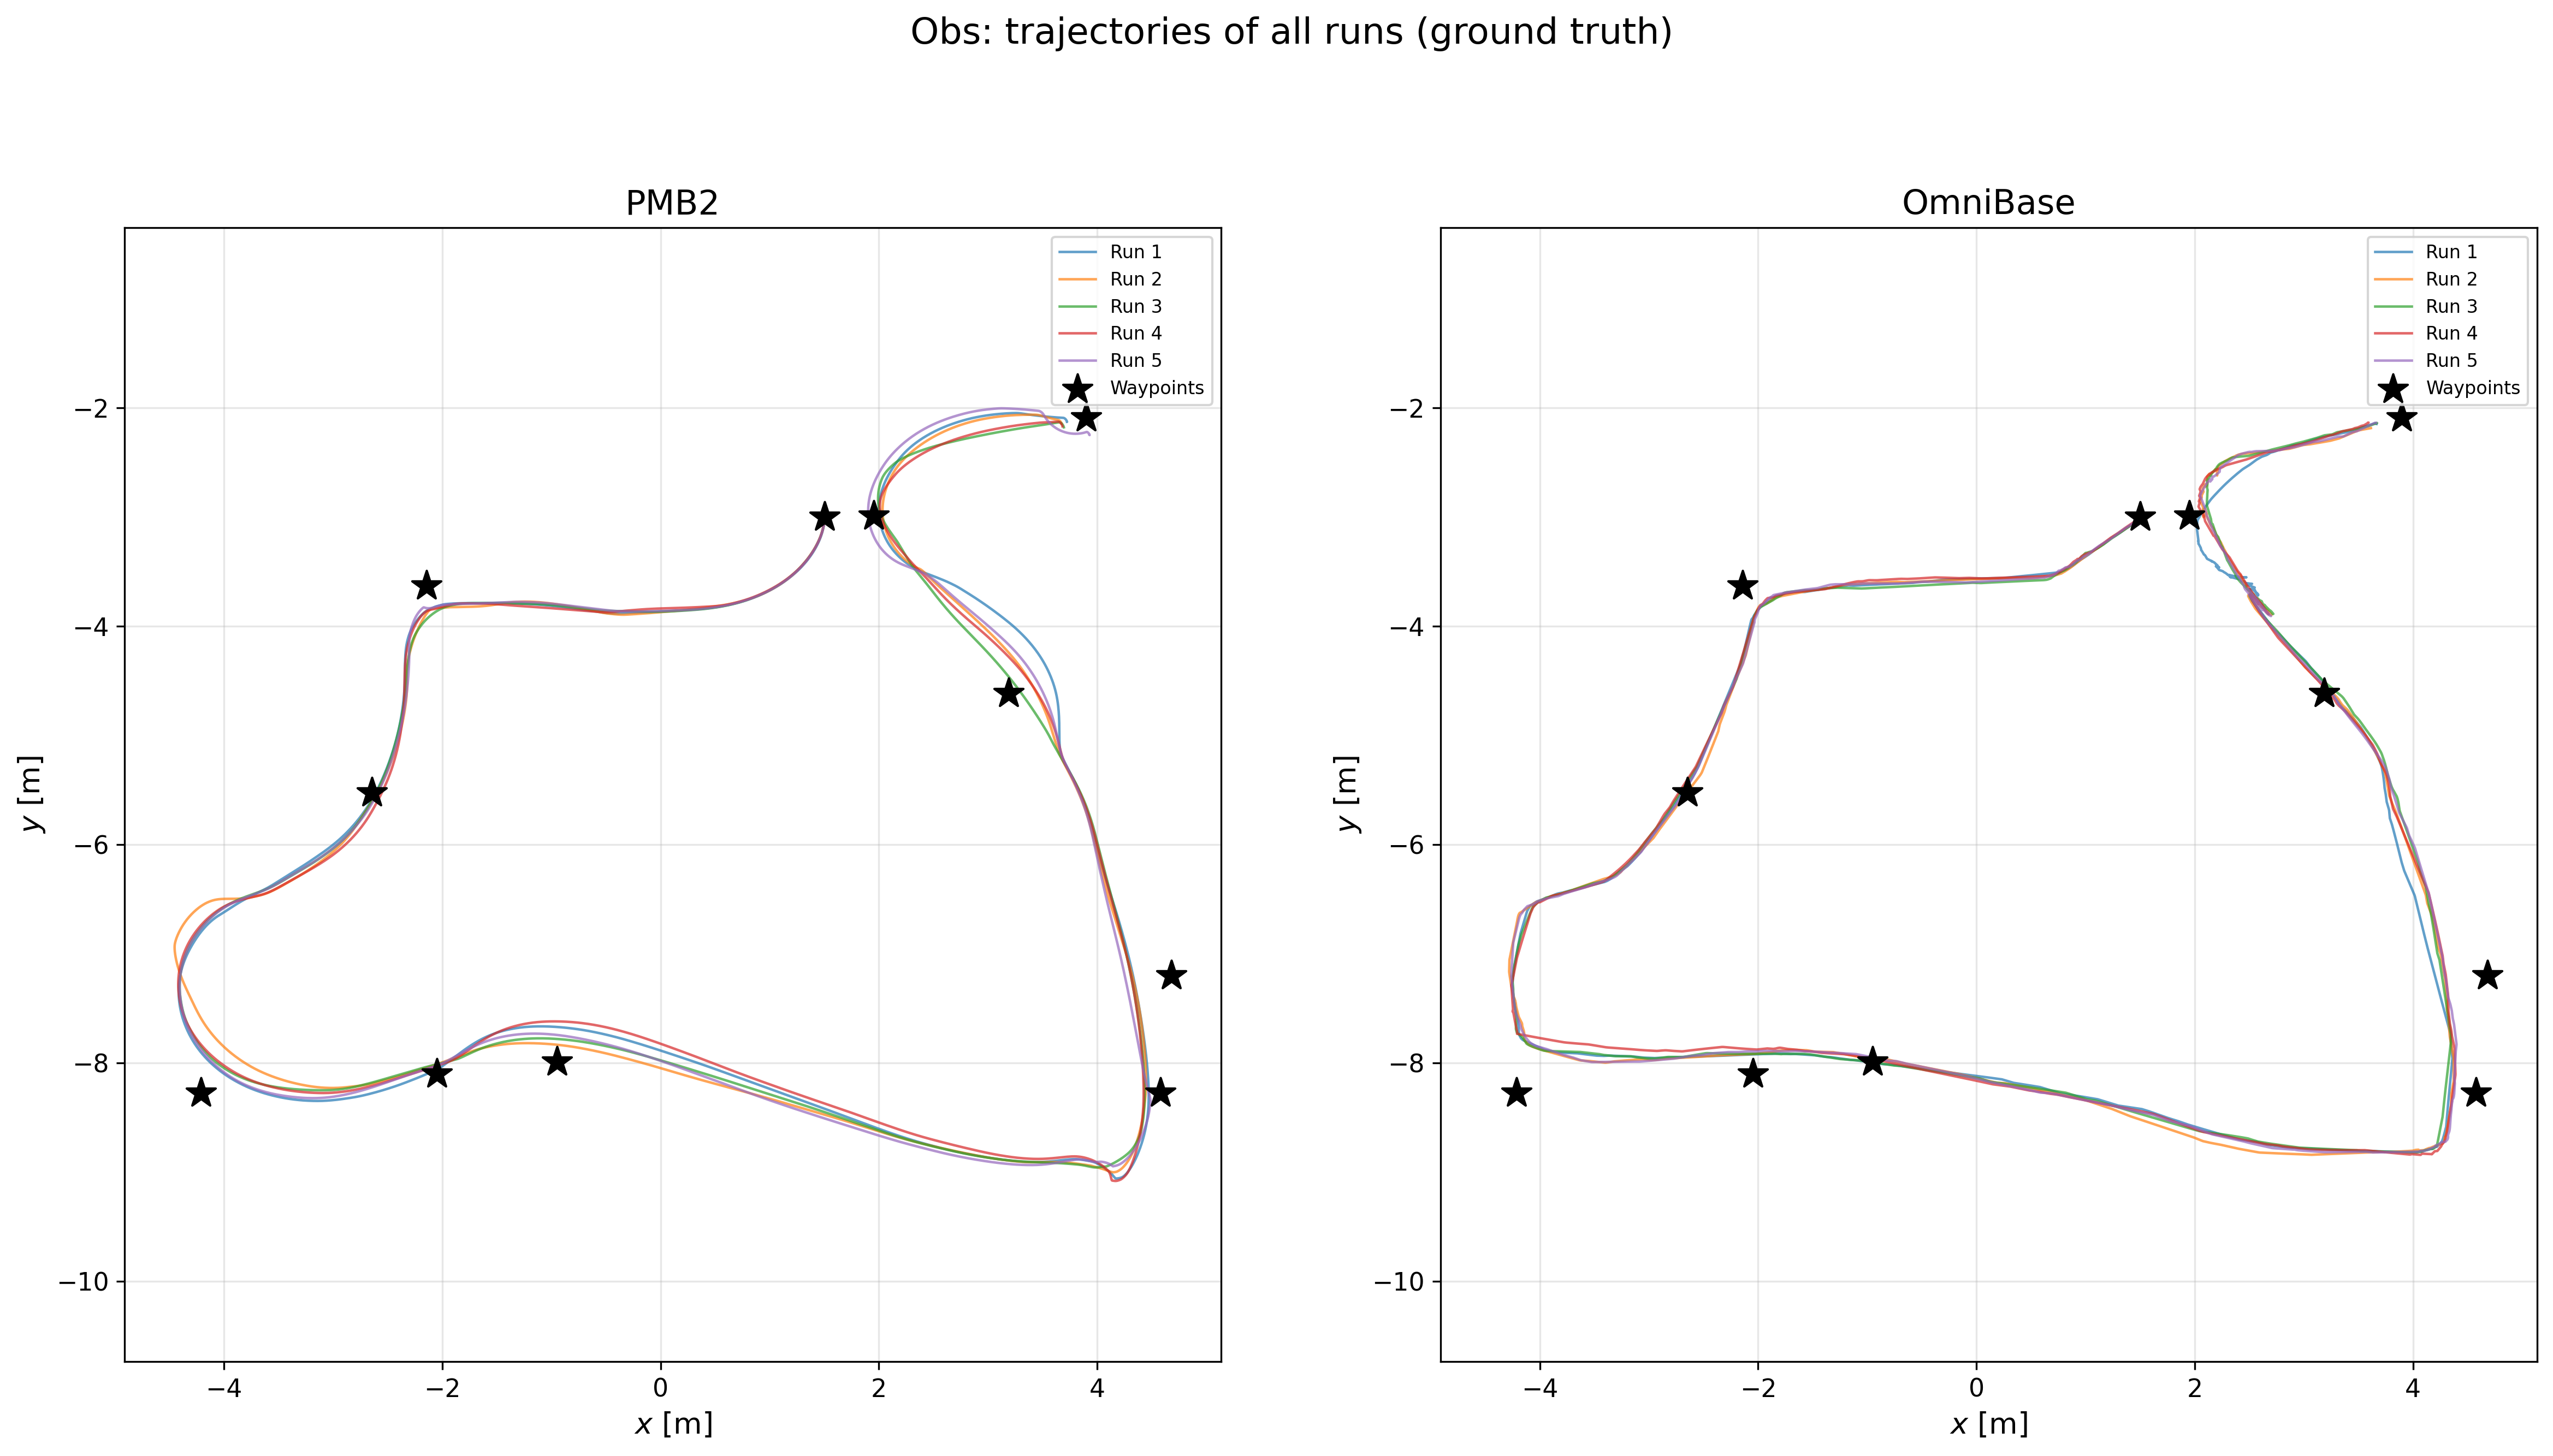
\includegraphics[width=\textwidth]{images/Ch4/obs/trajectories_all_Obs.png}
  \caption{Cluttered obstacle course: Ground~Truth trajectories of all five runs per base. Both platforms complete the winding circuit through all eleven waypoints; the OmniBase runs (right) overlap slightly more tightly than the PMB2 ones (left).}
  \label{fig:obs-traj}
\end{figure}

The robustness gap is quantified in Figure~\ref{fig:obs-recov}. The headline is the planning-failure asymmetry already noted: a mean of $2.40$ failures per run for the differential base against none for the holonomic one. The interpretation requires care, however, and the recovery breakdown is instructive. The differential base never triggered a Spin, BackUp, or Wait: its difficulty manifested purely as failed global plans, each followed by a costmap-clearing action and a replan. The holonomic base shows the opposite signature---zero planning failures, but a small number of Spin, BackUp, and Wait actions. These are not spread across its runs: they belong almost entirely to a single anomalous run in which the OmniBase became temporarily stuck (the outlier that also inflates its mean completion time to $86.1$~s, against a median close to the PMB2's $75.6$~s). Holonomy therefore did not make the platform immune to getting stuck, but it did prevent the global planner from ever failing.

\begin{figure}[htbp]
  \centering
  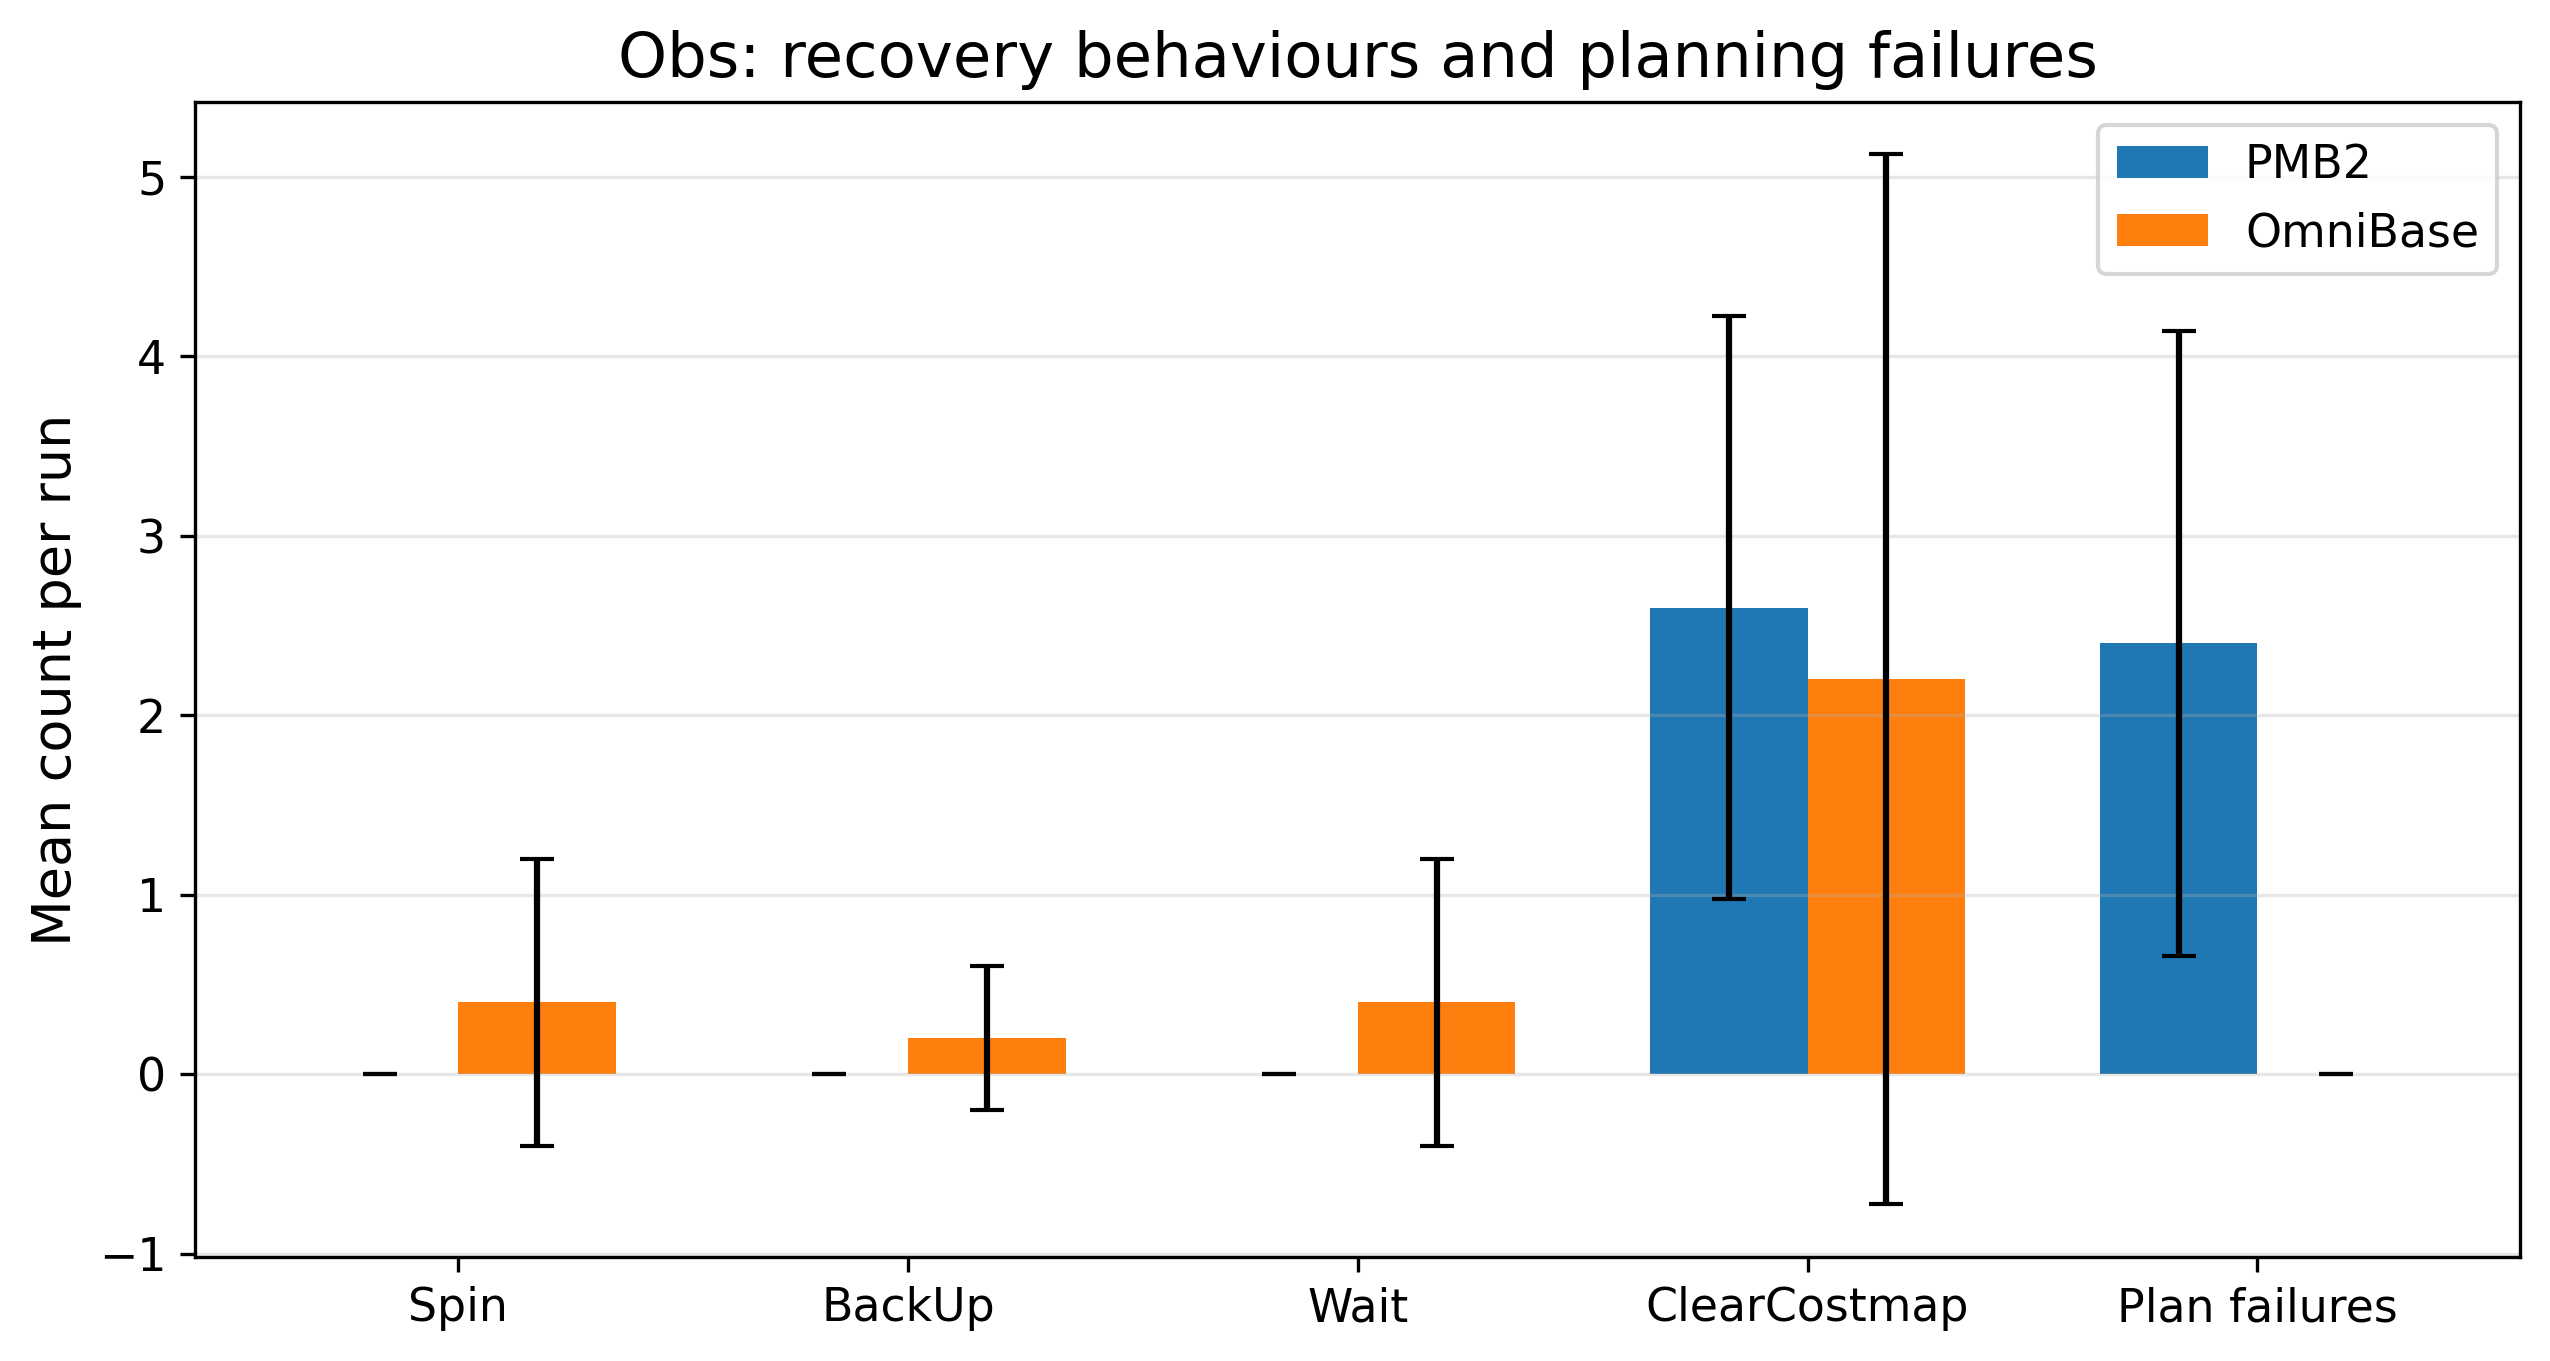
\includegraphics[width=0.9\textwidth]{images/Ch4/obs/recovery_counts_Obs.png}
  \caption{Cluttered obstacle course: recovery behaviours and planning failures, mean per run over five runs. The differential base fails to plan repeatedly (rightmost group) but never invokes Spin, BackUp, or Wait; the holonomic base never fails to plan, its few manoeuvre recoveries originating almost entirely from a single stuck run.}
  \label{fig:obs-recov}
\end{figure}

Figure~\ref{fig:obs-recovmap} reveals \emph{where} this struggle occurs. For the differential base the costmap-clearing actions are not scattered along the route but cluster at its tightest passage---the narrow section where the circuit doubles back close to its own starting point---indicating that the global planner repeatedly failed to route the non-holonomic footprint through that gap and had to clear the costmap and retry. The holonomic base cleared its costmap only once, at the same pinch point. This is the spatial fingerprint of the kinematic difference: at a narrow passage the holonomic base can side-step laterally into a valid trajectory, so a feasible plan is almost always found, whereas the differential base, which must rotate before it can translate, more often finds no admissible plan and falls back on the recovery pipeline.

\begin{figure}[H]
  \centering
  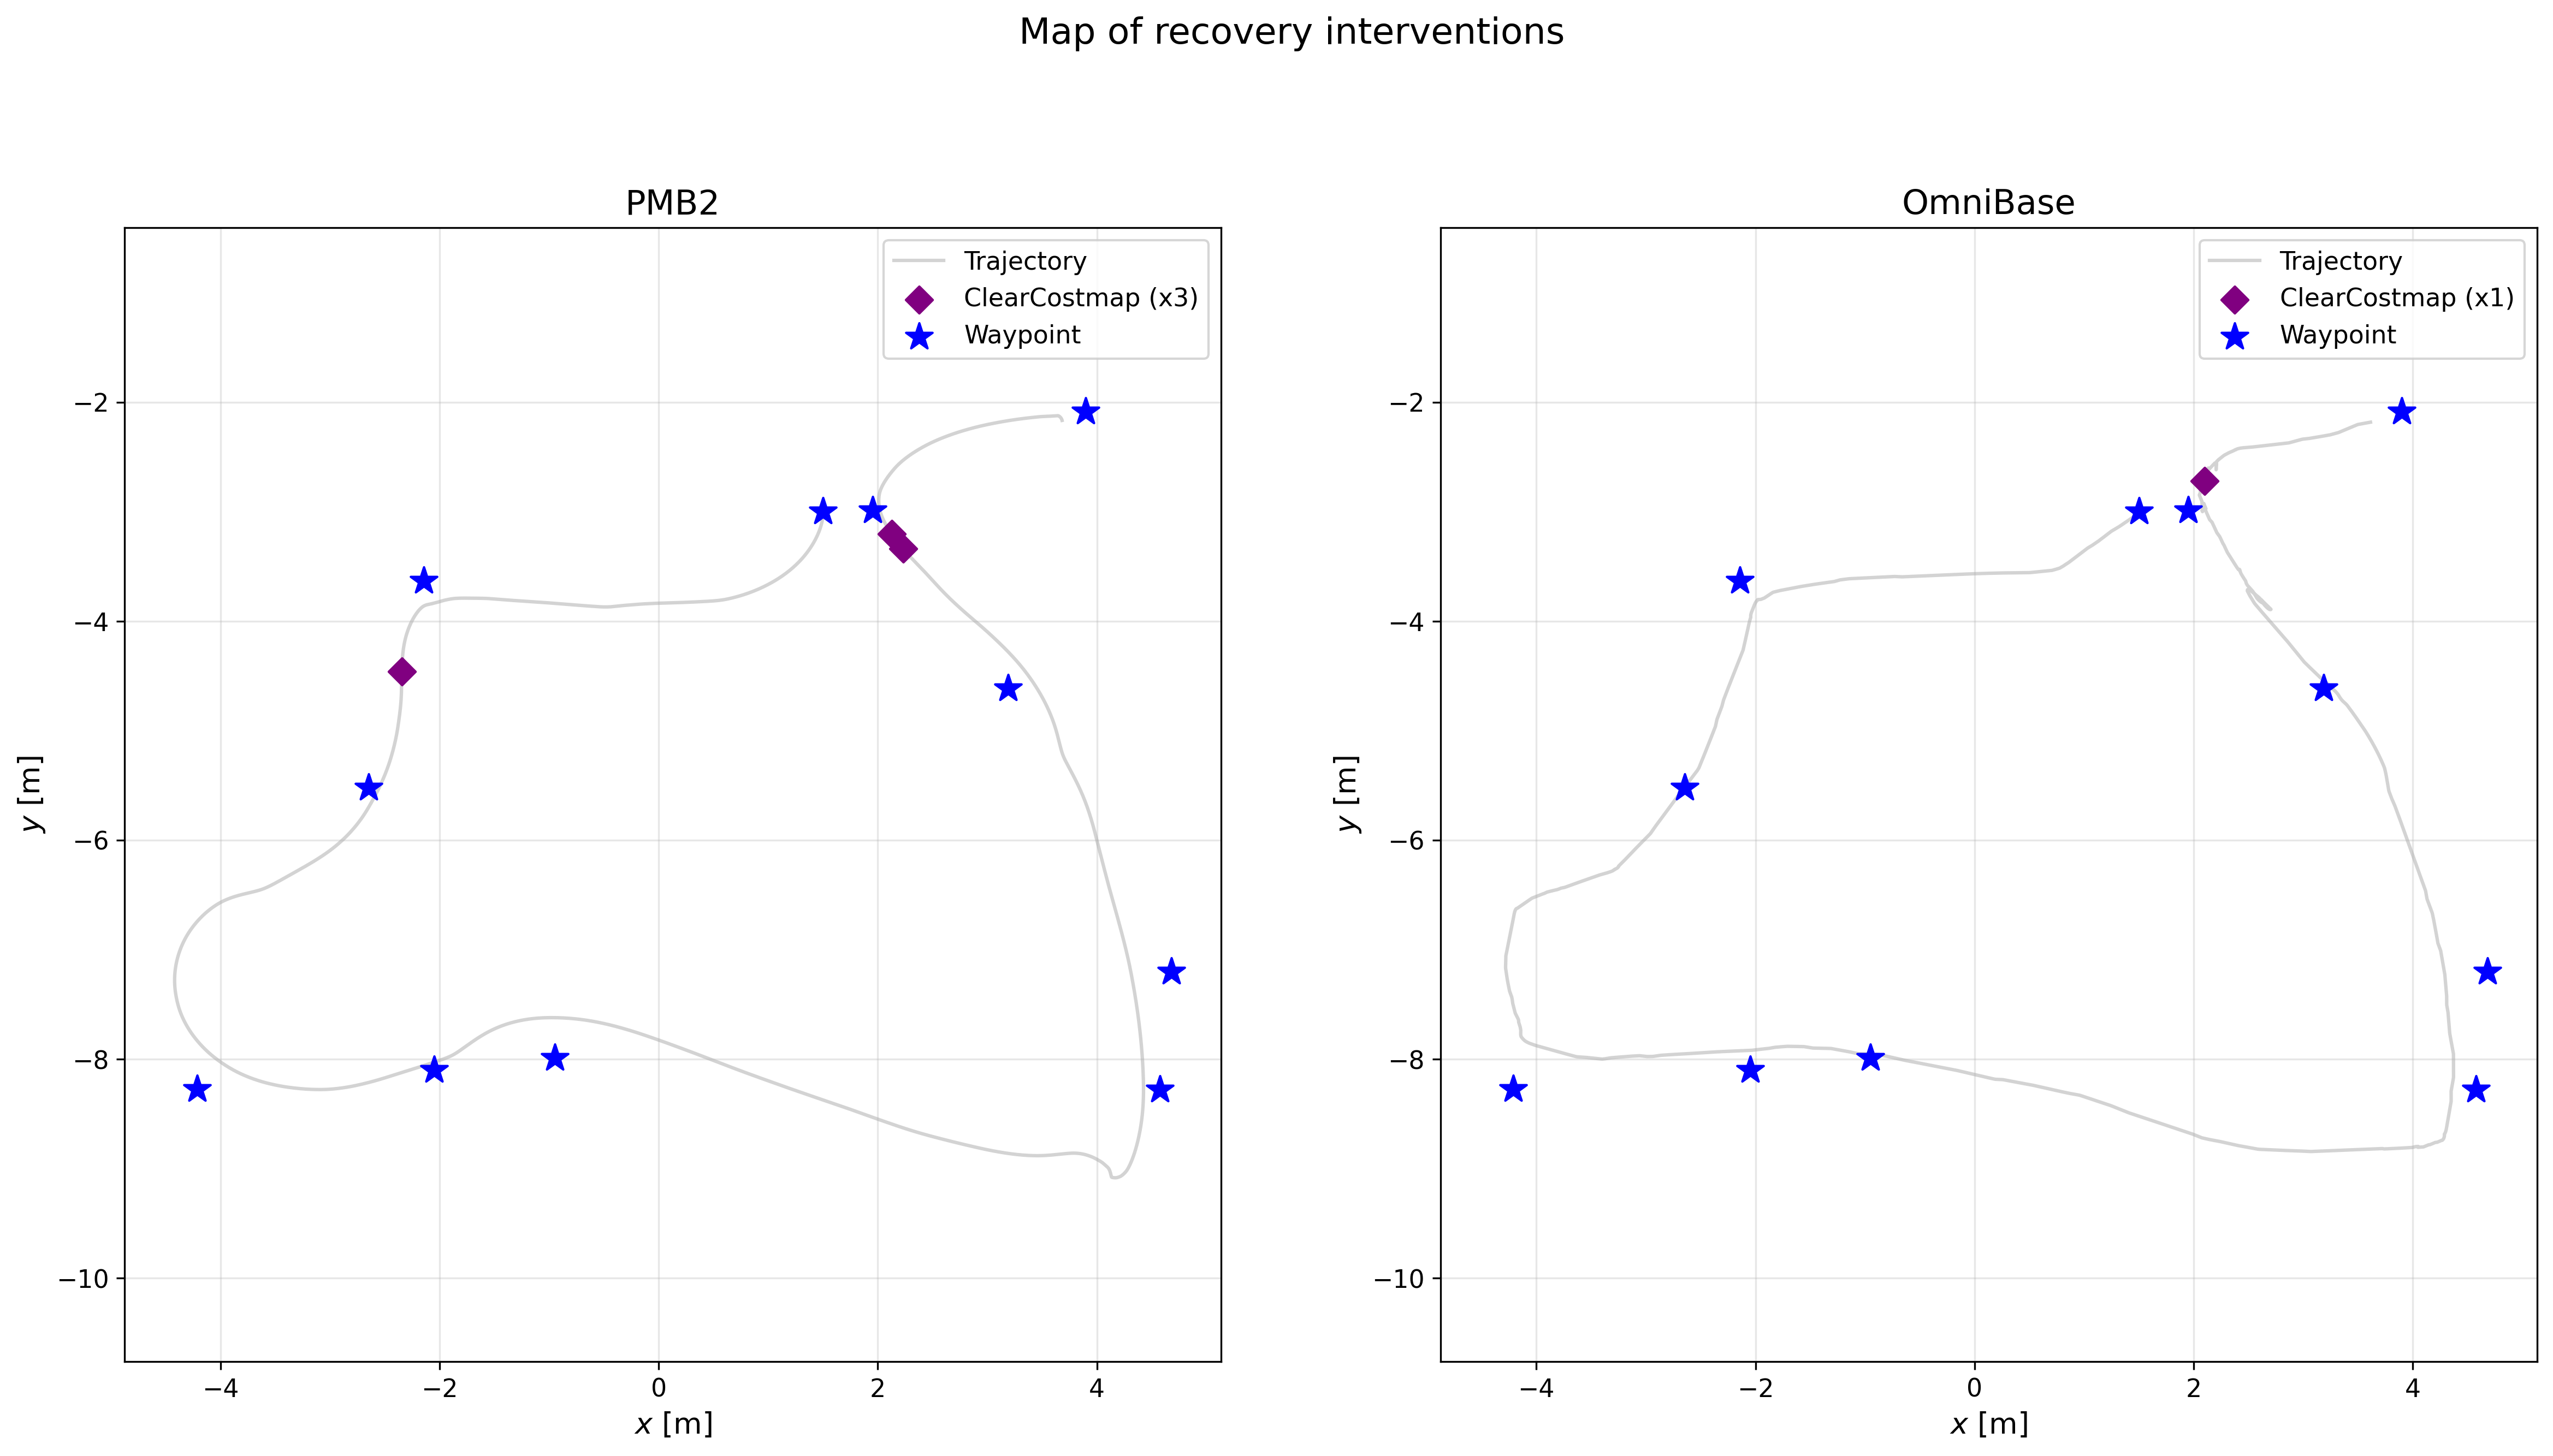
\includegraphics[width=\textwidth]{images/Ch4/obs/recovery_map.png}
  \caption{Cluttered obstacle course: location of the costmap-clearing actions for a representative run of each base (three for the PMB2, one for the OmniBase). The differential base's clears cluster at the narrowest passage of the circuit, where routing its footprint repeatedly failed.}
  \label{fig:obs-recovmap}
\end{figure}

\begin{figure}[H]
  \centering
  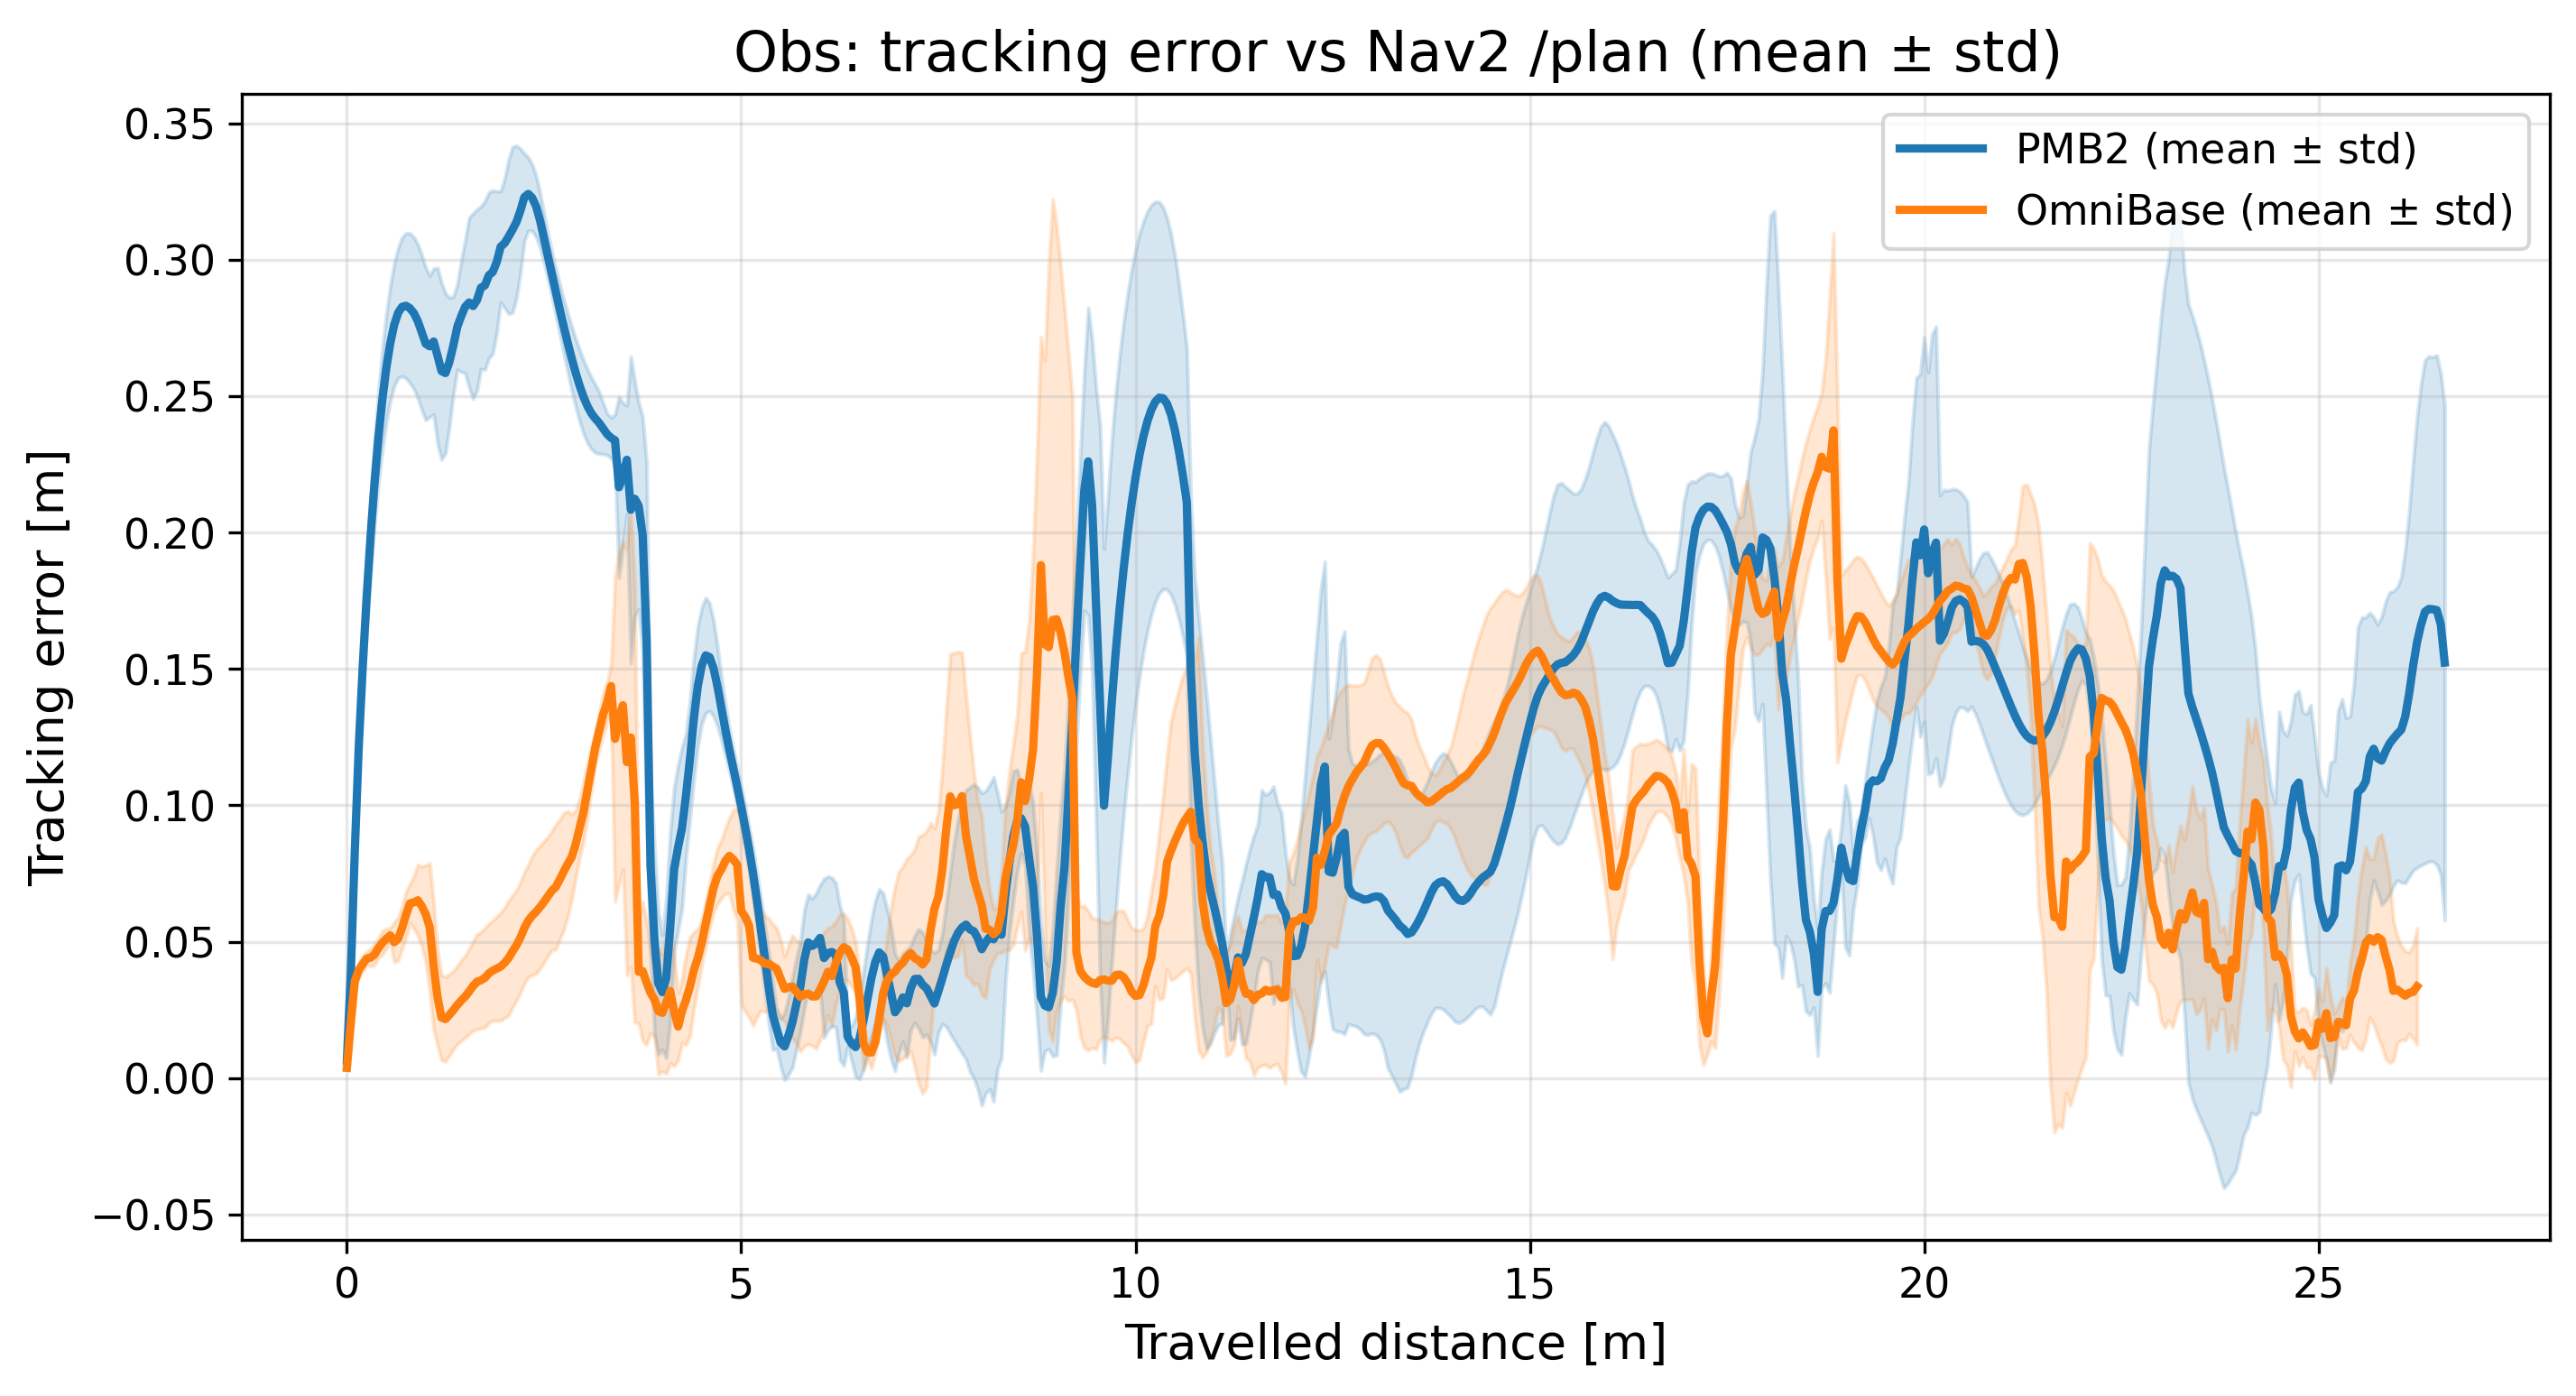
\includegraphics[width=1\textwidth]{images/Ch4/obs/cross_track_band_Obs.png}
  \caption{Cluttered obstacle course: tracking error against the Nav2 global plan as a function of travelled distance (mean $\pm$ standard deviation over five runs). Unlike the smooth growth observed on the straight corridor, both profiles are markedly jagged, reflecting the many tight manoeuvres the clutter demands; the holonomic OmniBase remains lower on average.}
  \label{fig:obs-xtrack}
\end{figure}

Beyond robustness, the route confirms the tracking and effort patterns seen earlier. As on the straight corridor, the holonomic base follows the planned path more closely on average (mean tracking error $0.068$ against $0.136$~m), correcting deviations laterally. As Figure~\ref{fig:obs-xtrack} shows, however, the tracking-error profiles of both bases are now markedly jagged---in contrast to the smooth accumulation seen on the corridor---reflecting the many tight manoeuvres the clutter demands. The waypoint positioning errors are comparable between the platforms ($0.175$ against $0.187$~m) and vary from waypoint to waypoint according to the local corner-cutting geometry, with no consistent winner. The clearest separation is in angular effort: over eleven waypoints the differential base is almost continuously re-orienting, which yields an angular smoothness more than twice as large as the holonomic base's ($2.833$ against $1.217$~rad/s$^2$) and a large mean orientation error ($1.670$~rad)---the latter again reflecting the constantly changing heading of a base that must turn in order to move, rather than a failure to reach commanded orientations (Section~\ref{subsec:m-accuracy}). The holonomic base instead holds its heading and relies on lateral motion (lateral usage $0.649$).

In summary, the obstacle course inverts the lesson of the sharp corner. There, holonomy bought speed; here, on a long cluttered route requiring frequent reorientation from both platforms, the completion times are comparable on the median and holonomy instead buys \emph{robustness}---no planning failures and tighter path adherence---together with far lower angular effort. The recurring theme is the fragility of the differential base's planning in confined spaces, a fragility that, as the next section shows, reappears in the autonomous-exploration pipeline. As throughout, the absolute smoothness and variance figures remain subject to the actuation-fidelity caveat of Section~\ref{subsec:m-fidelity}.

\section{Autonomous Exploration Results}
\label{sec:expl-results}

This section reports the autonomous frontier-based exploration of the \texttt{home} apartment, the second navigation pipeline of this study. Both platforms completed all five runs, each terminating on the frontier-exhaustion criterion of Section~\ref{subsec:expl-protocol} after mapping essentially the whole apartment. The outcome is more nuanced than a simple ordering: as summarised in Table~\ref{tab:explore}, the two bases reach an equivalent final coverage, but the differential PMB2 covers the environment faster and more efficiently, while the holonomic OmniBase is far more robust in planning and more stable in localisation. The planning fragility already observed on the cluttered waypoint route (Section~\ref{subsec:res-obstacles}) reappears here in an even more pronounced form.

\begin{table}[htbp]
\centering
\caption{Autonomous exploration: aggregate metrics, mean $\pm$ standard deviation over five runs.}
\label{tab:explore}
\begin{tabular}{lcc}
\toprule
Metric & PMB2 (differential) & OmniBase (holonomic) \\
\midrule
Exploration time [s]           & $281.2 \pm 14.1$ & $365.0 \pm 48.3$ \\
Time to target area [s]        & $224.4 \pm 40.1$ & $315.6 \pm 43.7$ \\
Final mapped area [m$^2$]      & $255.7 \pm 2.8$ & $250.1 \pm 1.8$ \\
Path length [m]                & $58.3 \pm 11.5$ & $61.7 \pm 9.1$ \\
Efficiency [m$^2$/m]           & $4.52 \pm 0.68$ & $4.13 \pm 0.54$ \\
Efficiency [m$^2$/s]           & $0.91 \pm 0.05$ & $0.70 \pm 0.11$ \\
SLAM error, mean [m]           & $0.176 \pm 0.122$ & $0.096 \pm 0.012$ \\
SLAM error, max [m]            & $0.391 \pm 0.236$ & $0.239 \pm 0.042$ \\
Angular smoothness [rad/s$^2$] & $2.247 \pm 0.158$ & $1.220 \pm 0.044$ \\
Lateral usage                   & $0.000 \pm 0.000$ & $0.579 \pm 0.044$ \\
Planning failures              & $32.4 \pm 19.8$ & $0.0 \pm 0.0$ \\
Costmap clears                 & $24.4 \pm 11.6$ & $11.4 \pm 5.2$ \\
Spin / BackUp / Wait           & $3.8$ / $2.0$ / $3.0$ & $1.6$ / $0.2$ / $1.0$ \\
\bottomrule
\end{tabular}
\end{table}

\begin{figure}[H]
  \centering
  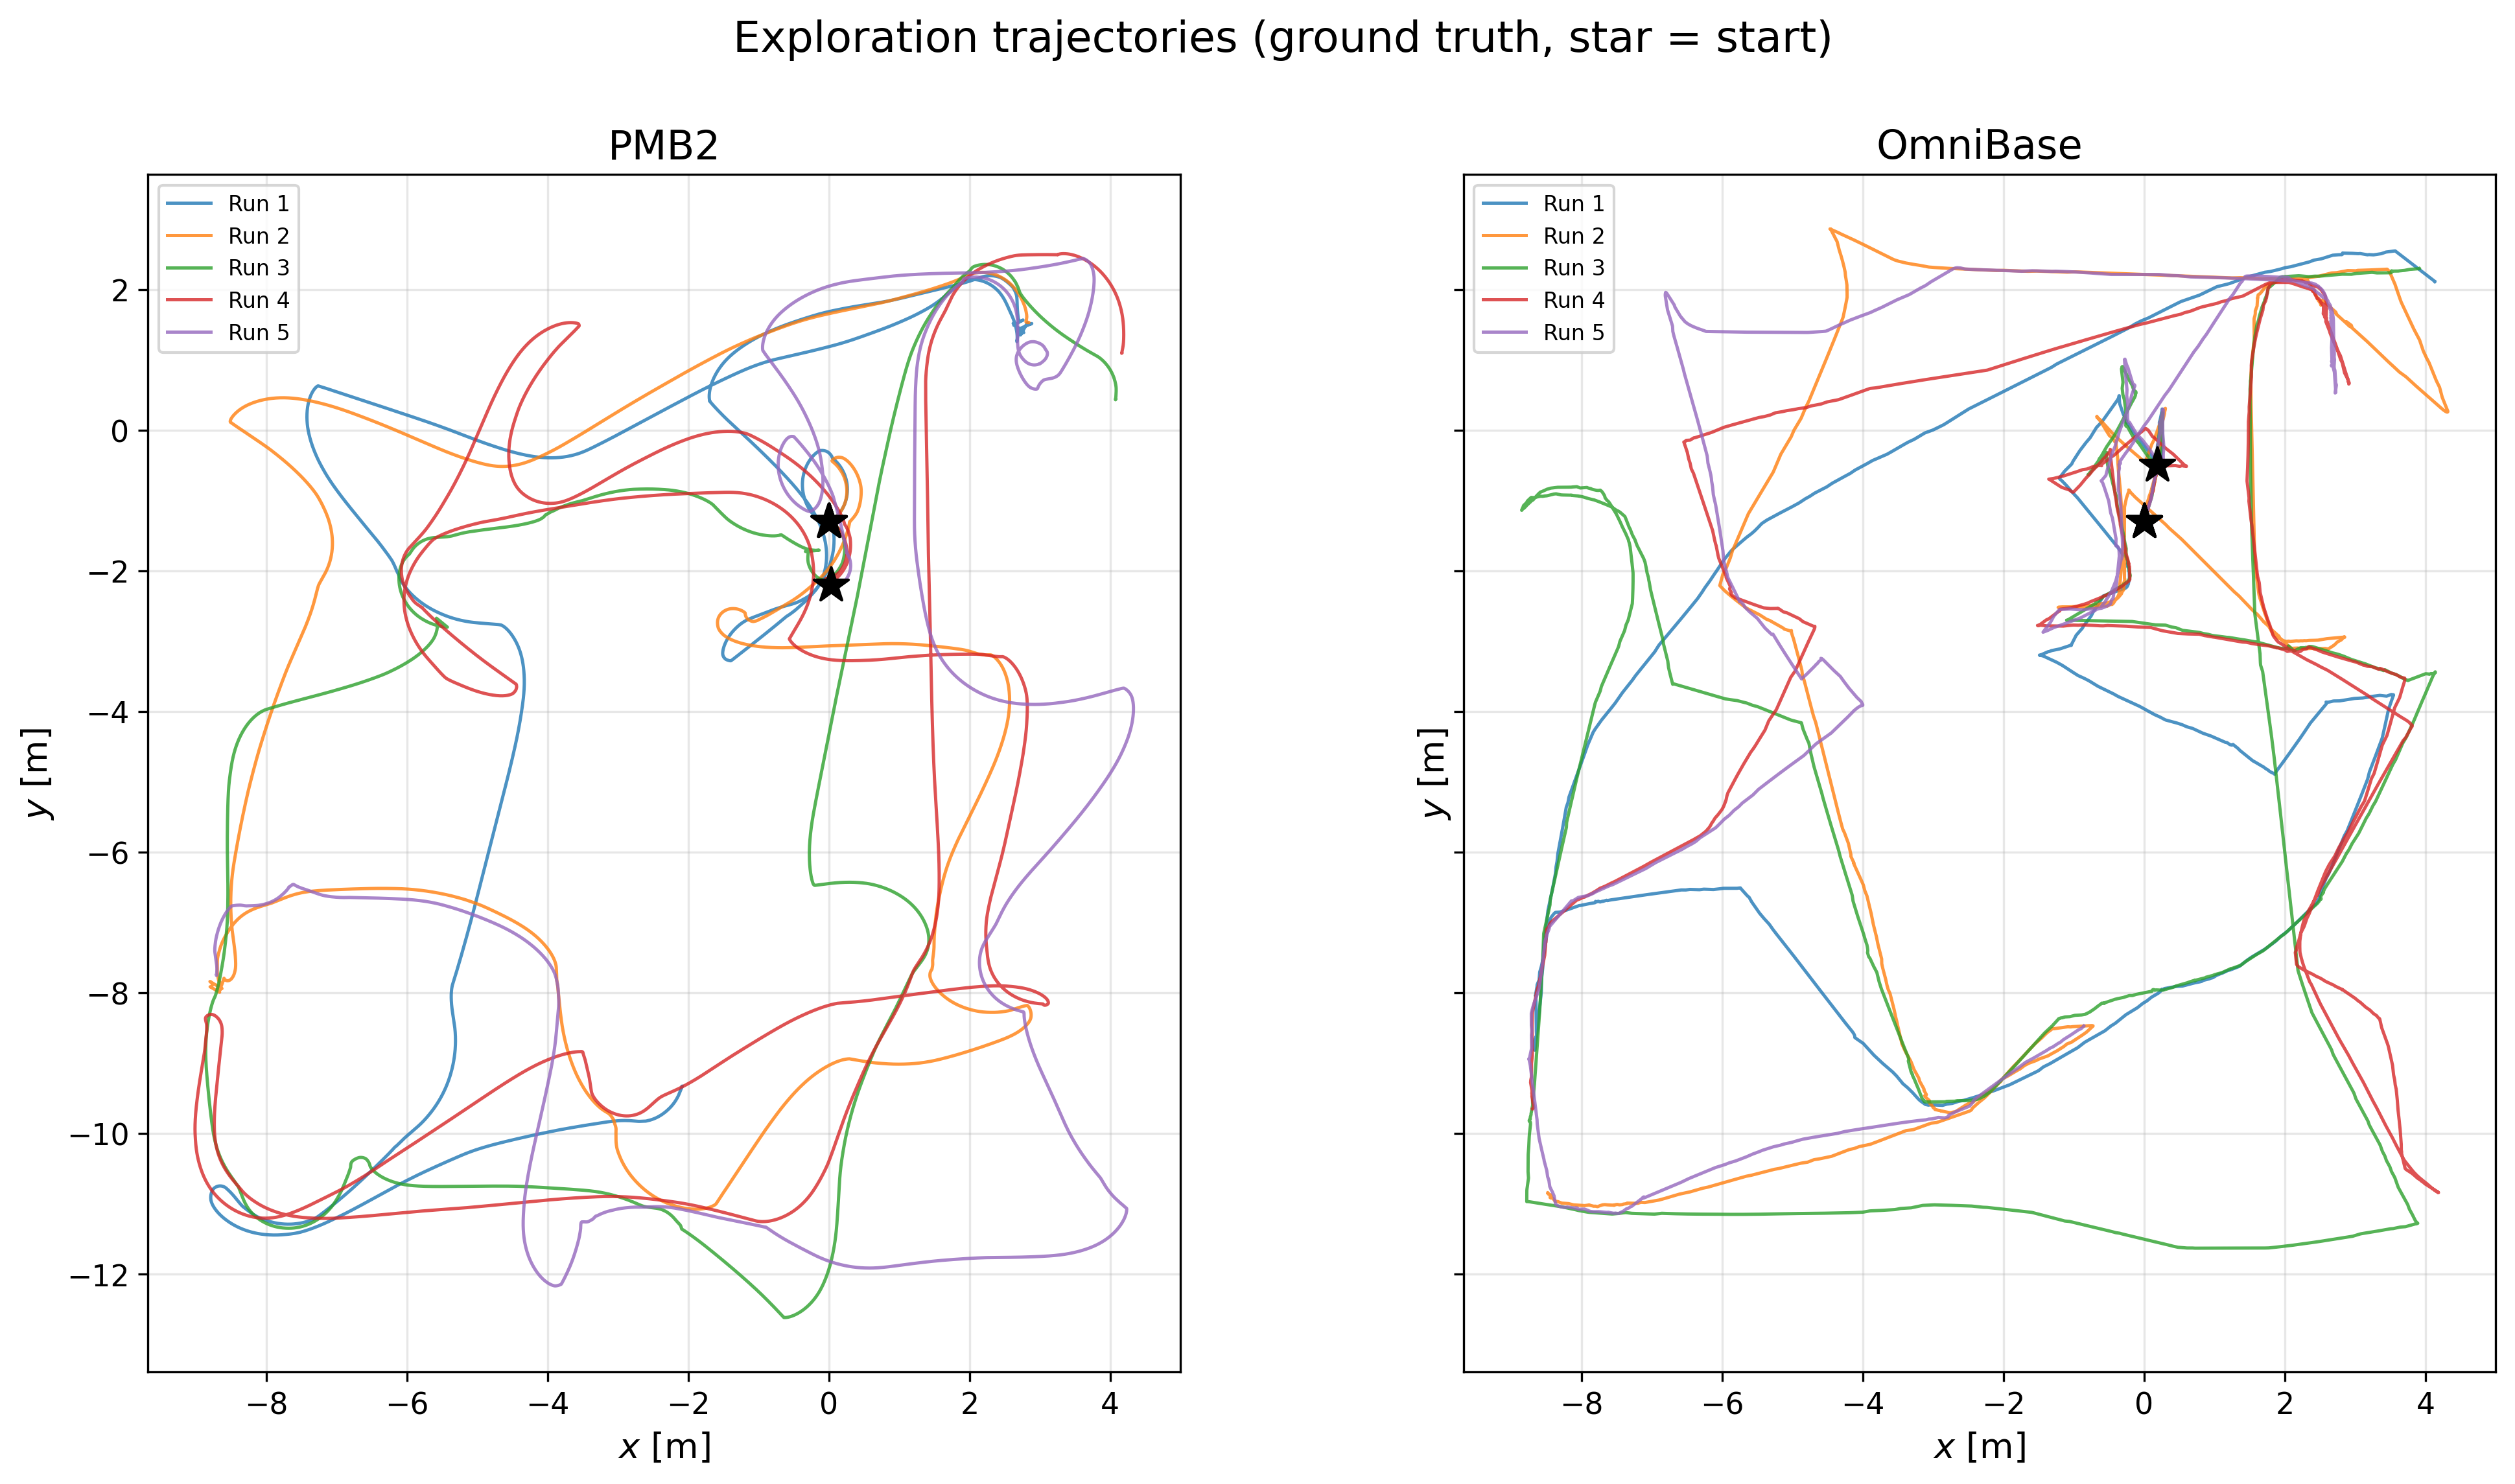
\includegraphics[width=\textwidth]{images/Ch4/expl/exploration_trajectories.png}
  \caption{Autonomous exploration: Ground~Truth trajectories of all five runs per base (stars mark the start pose). Both platforms traverse the entire apartment; the paths differ markedly from run to run, as expected from the frontier-selection process, which discovers and visits regions in a different order each time.}
  \label{fig:expl-traj}
\end{figure}

Figure~\ref{fig:expl-traj} shows that both platforms explore the whole apartment, and that---unlike the waypoint routes---the trajectories are not repeatable across runs: since the next goal depends on the frontiers currently visible in the incrementally built map, each run discovers the environment along a different path. This run-to-run variability is intrinsic to the task rather than a symptom of instability, and it is the reason the exploration campaign is characterised statistically over five repetitions.

\begin{figure}[H]
  \centering
  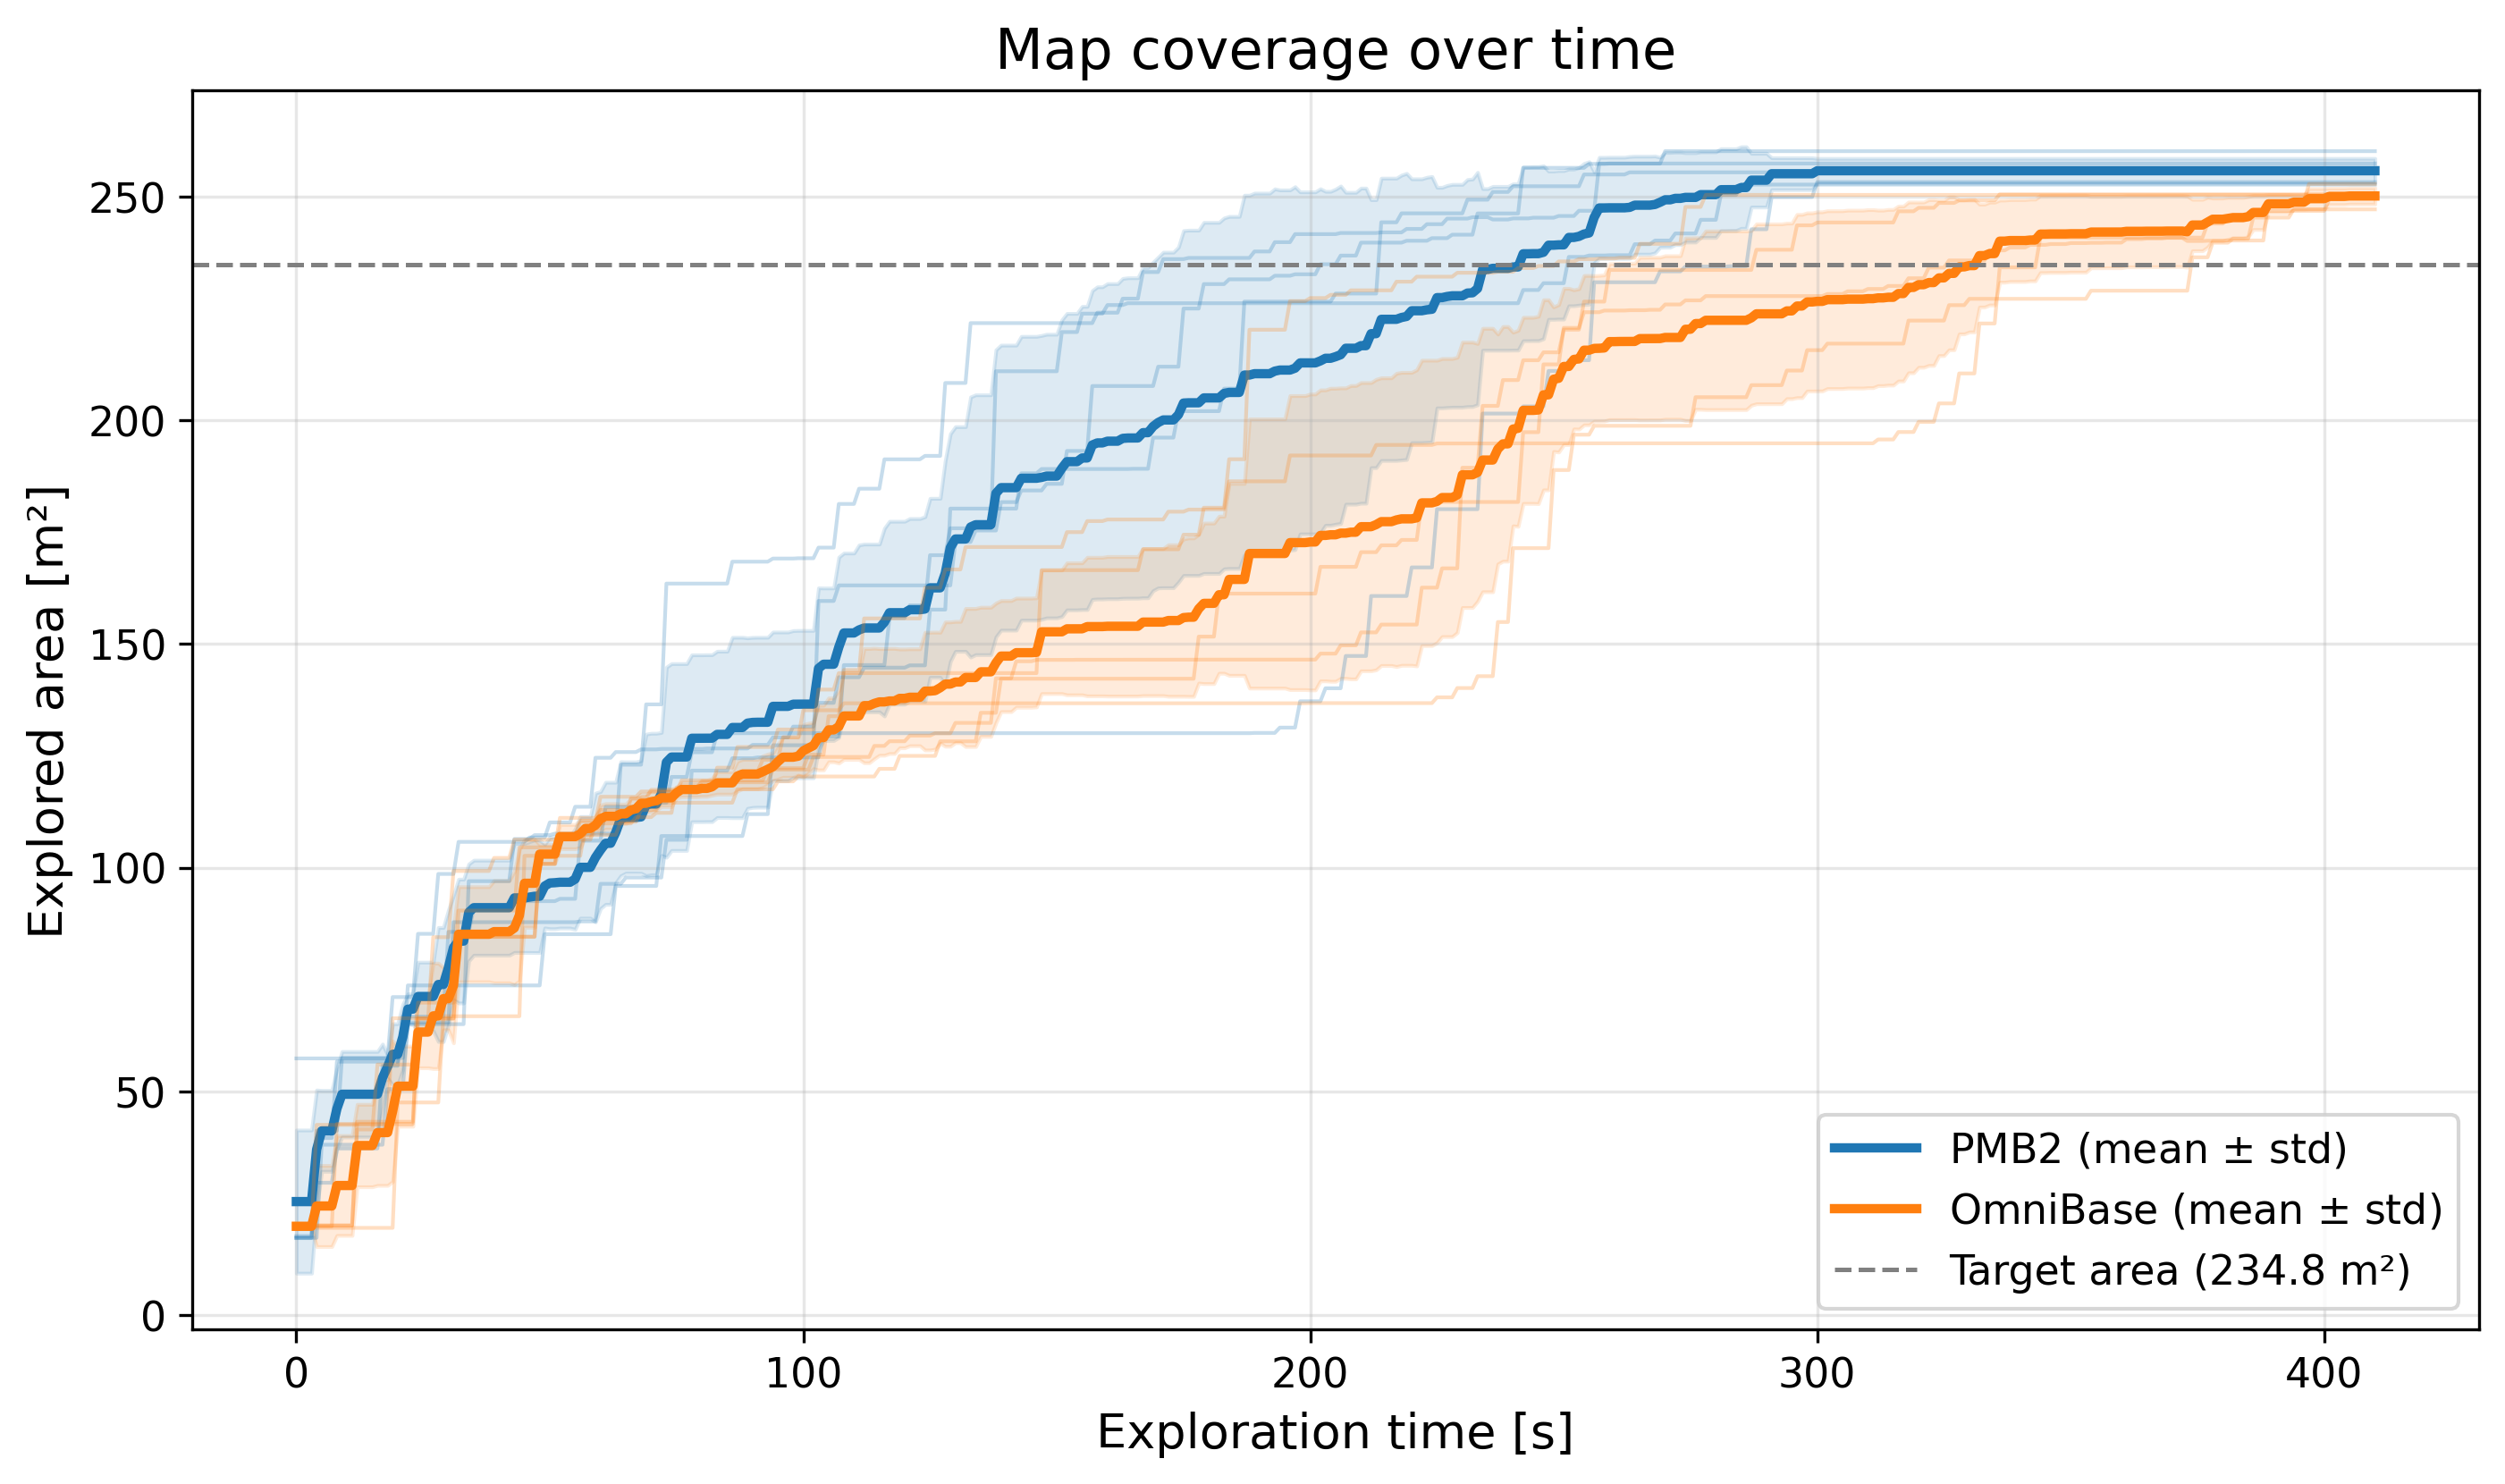
\includegraphics[width=1\textwidth]{images/Ch4/expl/coverage_vs_time.png}
  \caption{Autonomous exploration: mapped area as a function of exploration time (mean $\pm$ standard deviation over five runs). The differential PMB2 reaches the common target coverage (dashed line, $234.8$~m$^2$, i.e.\ $95\%$ of the smallest final area) earlier than the holonomic OmniBase; both converge to a similar final mapped area.}
  \label{fig:expl-coverage}
\end{figure}

In terms of coverage the differential base is the more effective of the two. Figure~\ref{fig:expl-coverage} shows its mapped area growing consistently faster: it reaches the common target coverage in $224$~s on average, against $316$~s for the holonomic base, and completes the whole exploration in $281$~s against $365$~s. The differential is also more efficient by both measures, covering more area per metre travelled ($4.52$ against $4.13$~m$^2$/m) and per second ($0.91$ against $0.70$~m$^2$/s), while the two platforms end at an equivalent final area ($255.7$ against $250.1$~m$^2$). This inverts the speed relationship seen at the sharp corner (Section~\ref{subsec:res-angle}). The reason lies in the geometry that the two bases must follow while mapping: much of the exploration consists of tracing long, narrow paths that skirt the apartment walls, often as elongated ``U''-shaped detours around a wall or into and out of a room. The differential PMB2, with its round footprint, negotiates such contours as wide, sweeping curves and traverses them quickly; the holonomic OmniBase, by contrast, has no manoeuvre to exploit along a wall---sideways motion offers no shortcut there---and its finer, closely-guided wall-following is comparatively slow. Since the open apartment rewards fast contour-following far more than lateral agility, the differential base covers the same area appreciably faster, while both reach an equivalent final extent. Figure~\ref{fig:expl-coverage} also shows that this gap does not open immediately: during the first $\sim$100~s the two coverage curves are almost indistinguishable, and the differential base pulls ahead only in the intermediate phase. This is consistent with the wall-following interpretation, as the initial coverage comes from the open central rooms---which both bases map at a similar rate---whereas the divergence appears once the exploration moves into the narrower, wall-bounded portions of the apartment that penalise the holonomic base.

\begin{figure}[H]
  \centering
  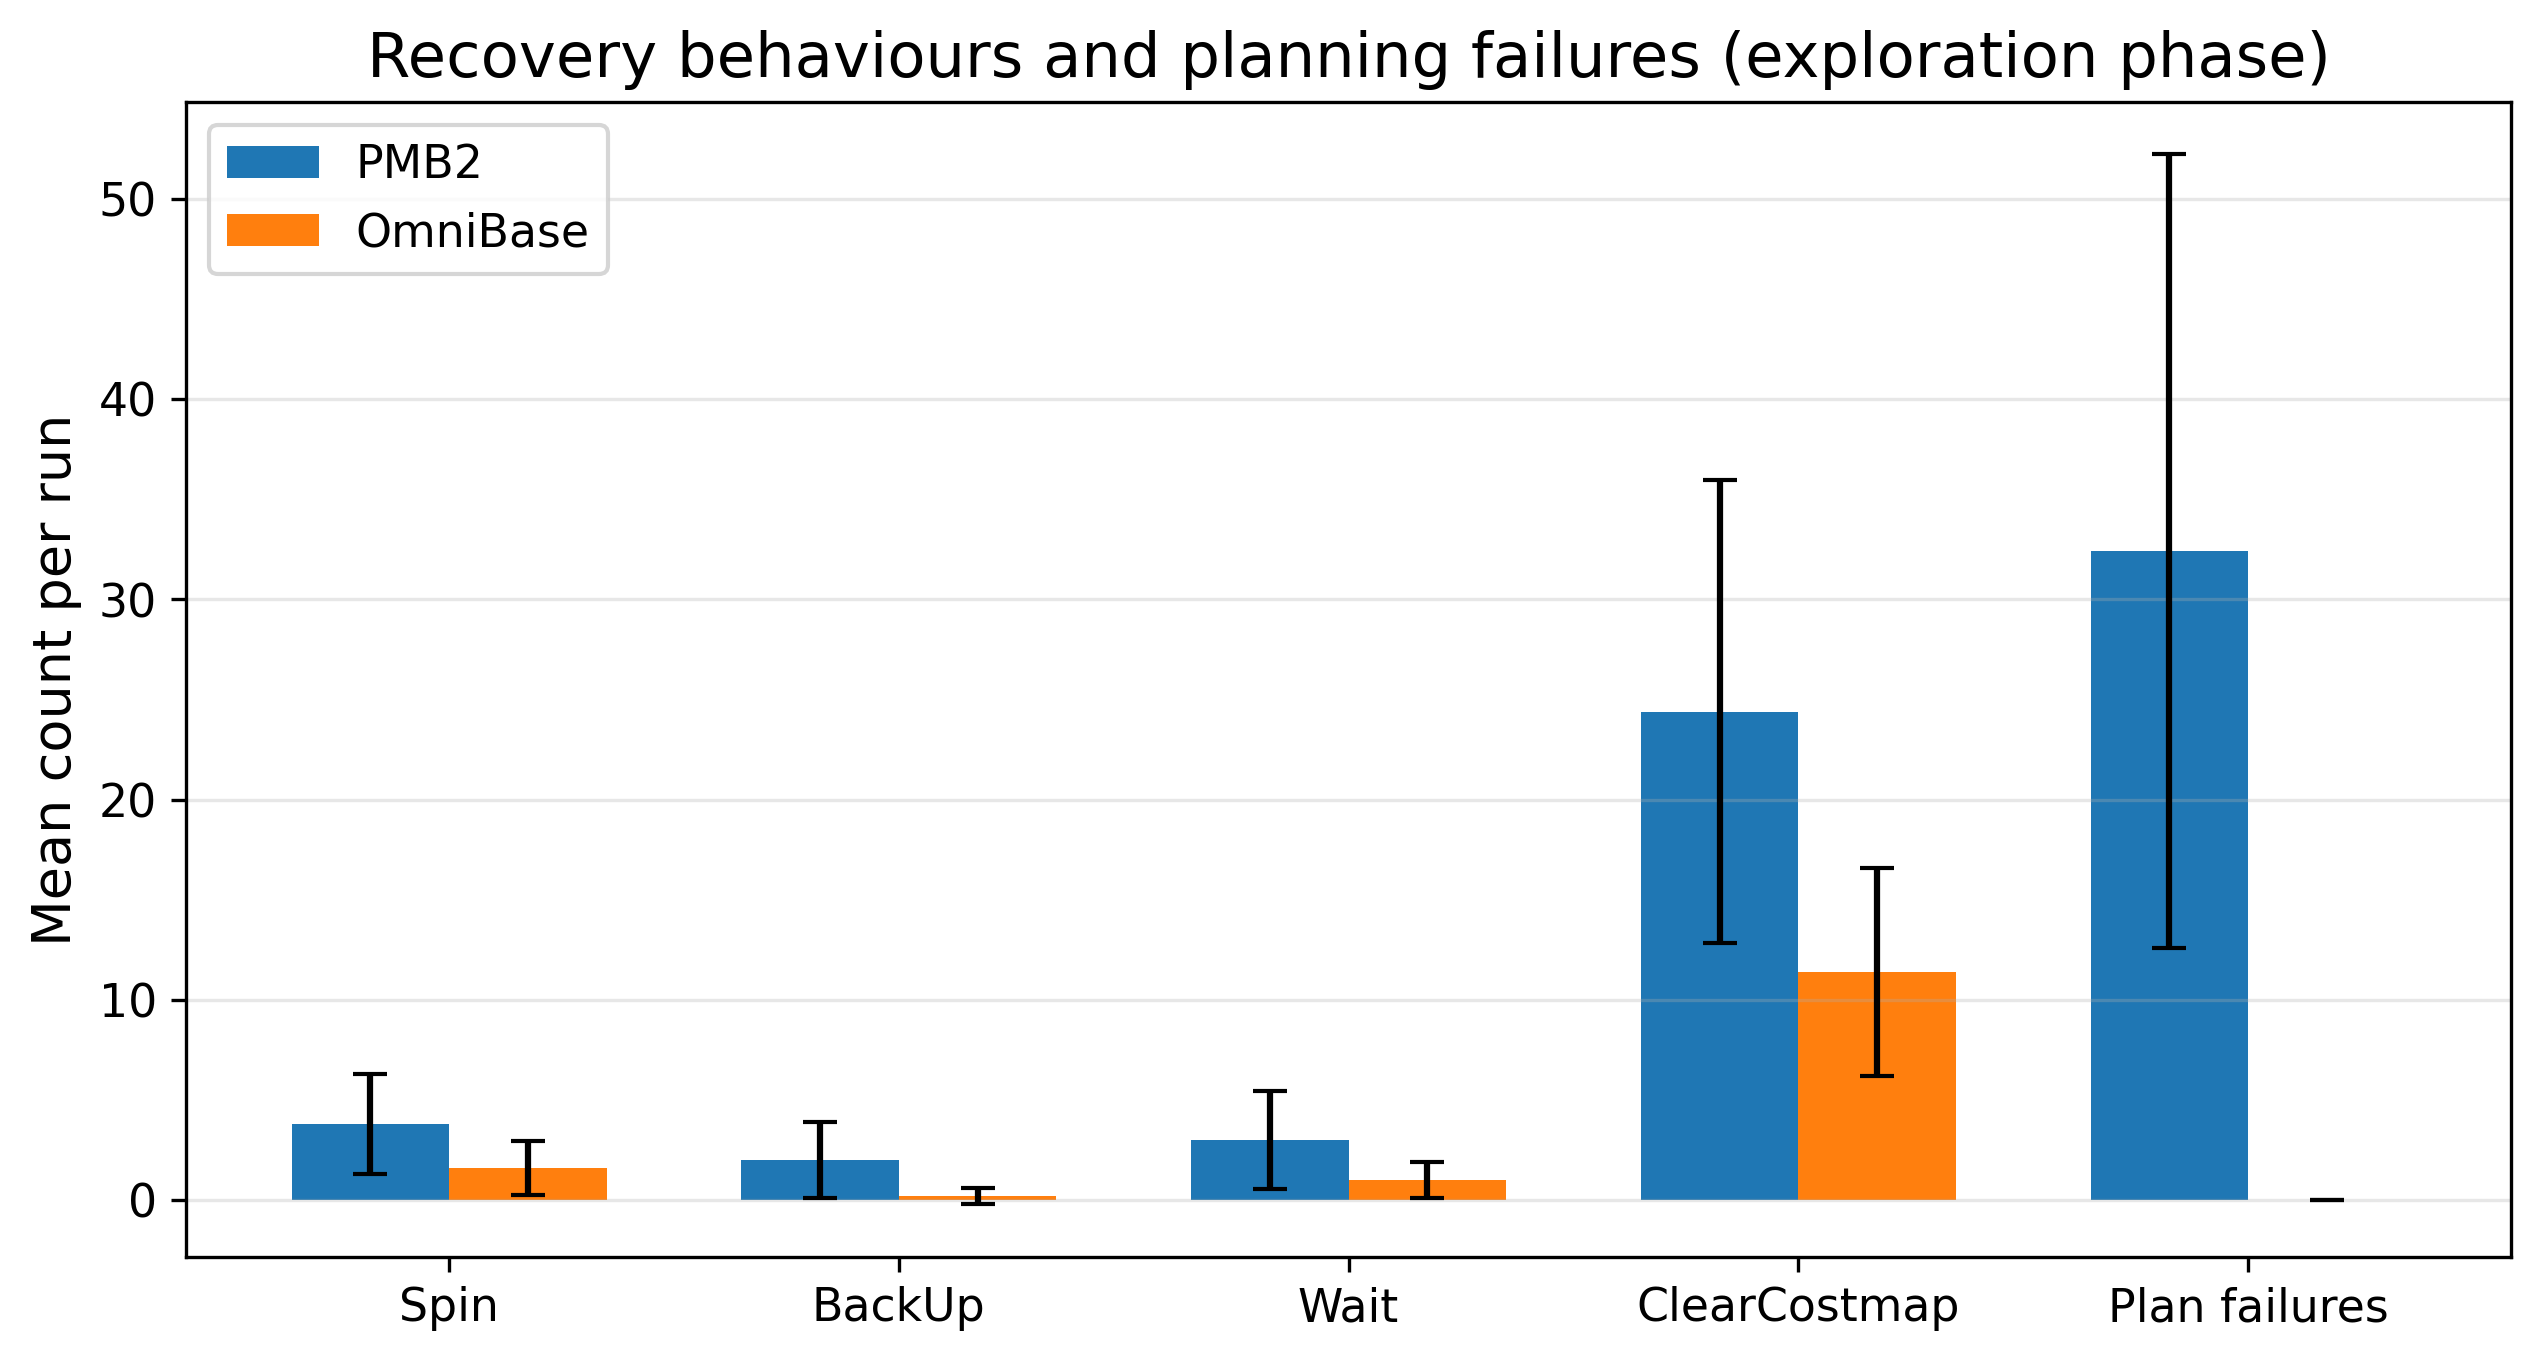
\includegraphics[width=1\textwidth]{images/Ch4/expl/recovery_counts.png}
  \caption{Autonomous exploration: recovery behaviours and planning failures, mean per run over five runs. The differential PMB2 incurs a large number of planning failures ($32.4$ per run on average) and more of every recovery action, whereas the holonomic OmniBase never fails to plan.}
  \label{fig:expl-recov}
\end{figure}

This coverage advantage, however, is bought at a steep price in robustness, and it is here that the central theme of the waypoint campaign re-emerges. As Figure~\ref{fig:expl-recov} shows, the differential base failed to produce a valid global plan an average of $32.4$ times per run---about $6\%$ of its planning attempts---while the holonomic base never failed once. The differential also triggered more of every recovery action, in particular clearing its costmap more than twice as often ($24.4$ against $11.4$). The mechanism is the same as on the obstacle course: the apartment mixes open rooms, which the differential crosses quickly, with narrow inter-room passages and doorways, through which routing a non-holonomic footprint repeatedly fails, forcing a costmap clear and a replan. The holonomic base negotiates the same passages by side-stepping into a feasible trajectory and therefore never exhausts the planner. Notably, these failures cost the differential time but not enough to erase its locomotion advantage: it still completes exploration faster despite recovering far more often.

\begin{figure}[H]
  \centering
  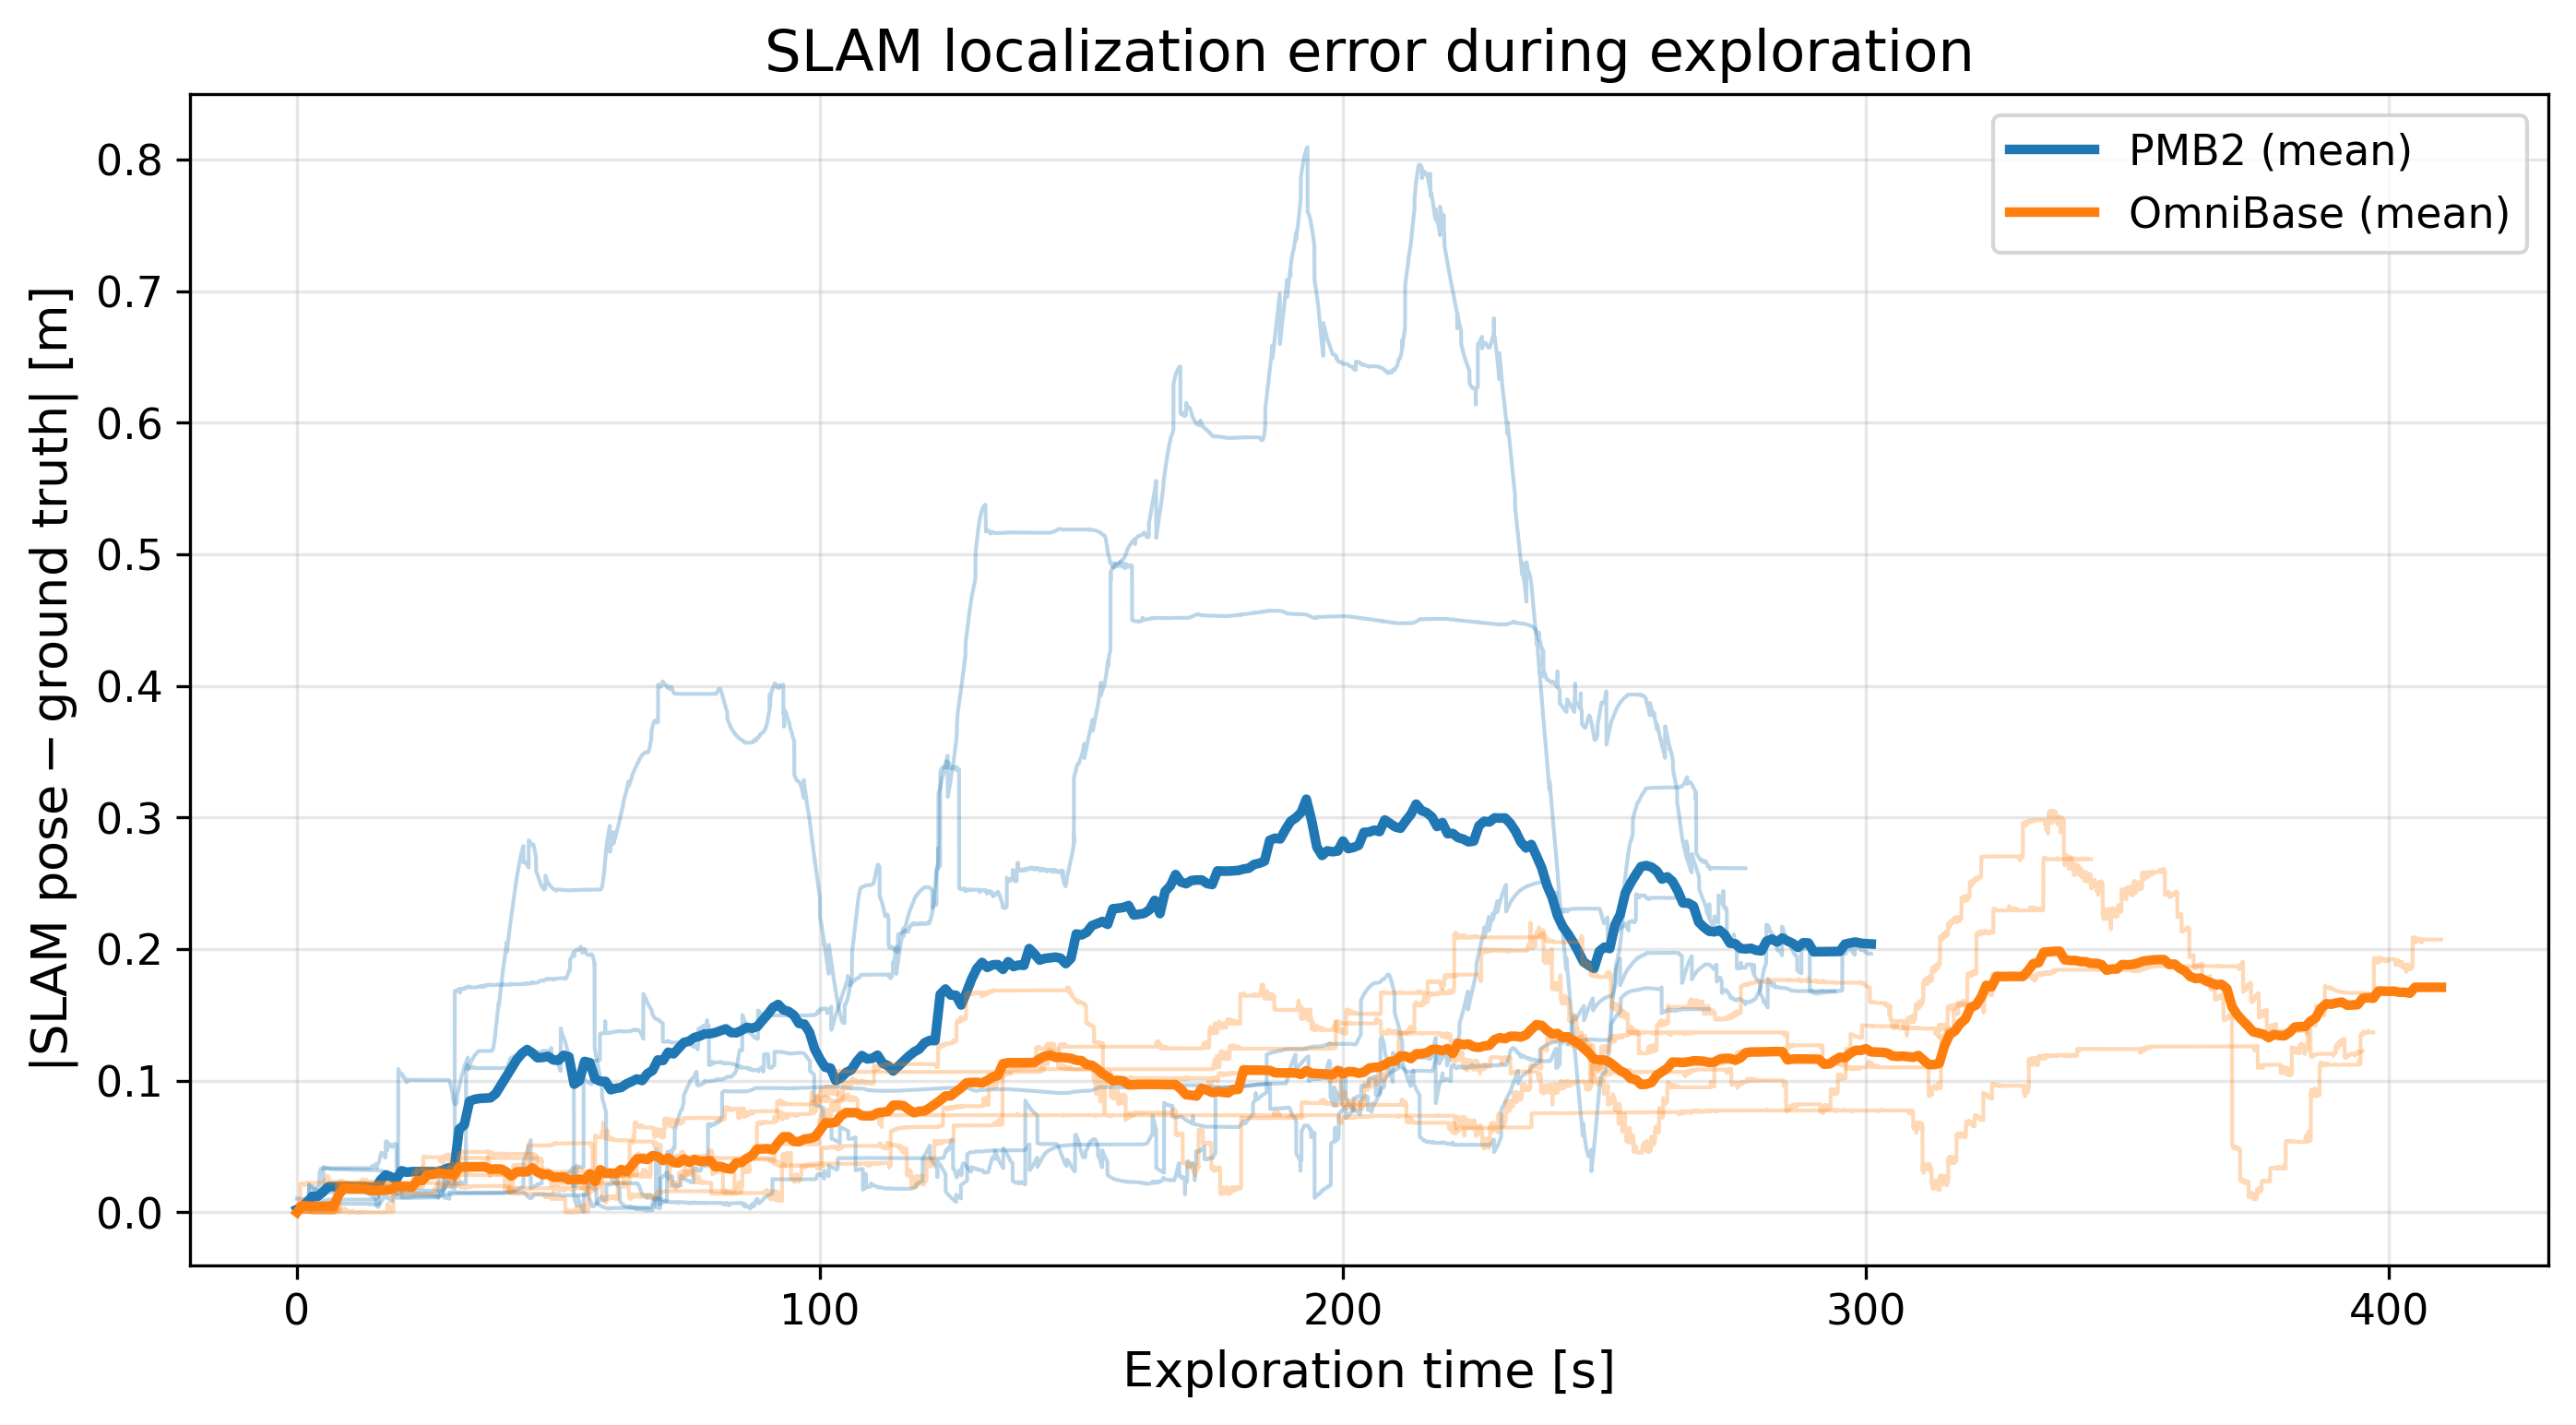
\includegraphics[width=1\textwidth]{images/Ch4/expl/slam_error_vs_time.png}
  \caption{Autonomous exploration: SLAM localisation error (distance between the \texttt{slam\_toolbox} estimate and Ground~Truth) over exploration time; bold lines are the per-base mean, faint lines the individual runs, after the map-to-world alignment of Section~\ref{subsec:m-exploration}. The holonomic OmniBase maintains a lower and far more consistent error, whereas the differential PMB2 is higher and highly variable, one run exceeding $0.8$~m. The OmniBase curves extend later in time, reflecting its longer exploration duration.}
  \label{fig:expl-slam}
\end{figure}

The second cost concerns localisation. Figure~\ref{fig:expl-slam} reports the error of the online SLAM estimate against Ground~Truth, after the per-run frame alignment described in Section~\ref{subsec:m-exploration}. The holonomic base maintains a low and remarkably consistent error (mean $0.096 \pm 0.012$~m), its five runs tightly bunched throughout. The differential base is both less accurate and dramatically less consistent (mean $0.176 \pm 0.122$~m, with a standard deviation almost as large as the mean): its error grows more steeply and its runs fan out widely, one exceeding $0.8$~m at its peak. Since both platforms run the same \texttt{slam\_toolbox} configuration, this difference reflects the interaction between the SLAM front-end and the two odometric regimes rather than a property of the mapping algorithm itself (Section~\ref{subsec:m-exploration}); the frequent in-place rotations of the differential base, and the drift they induce, are the most plausible source of its larger and more erratic localisation error, consistent with its markedly higher angular effort ($2.247$ against $1.220$~rad/s$^2$). This outcome may appear to run counter to the probabilistic analysis of Section~\ref{sec:probabilistic_motion_models}, which anticipated a broader, omnidirectional odometric uncertainty for the holonomic base and a more tightly constrained one for the differential. Two factors reconcile the two. First, that analysis concerns the raw odometric noise, whereas the error reported here is that of the full SLAM estimate: the additional lateral variance predicted for the OmniBase is precisely what the dedicated \texttt{alpha5} coefficient introduced in Section~\ref{subsec:amcl_tuning} is meant to bound. Second, and more decisively, what the scan-matching front-end of \texttt{slam\_toolbox} sees is the executed motion, and the OmniBase moves through long, smooth, heading-stable translations that are inherently favourable to registration, whereas the differential base interleaves its motion with the continual in-place rotations that its kinematics demand—the dominant source of pose drift for a laser SLAM system. The idealised, slip-free actuation of the OmniBase in simulation (Section~\ref{subsec:m-fidelity}) reinforces this effect and should be kept in mind: on physical hardware the lateral slippage of the Mecanum rollers would inject exactly the coupled noise that Section~\ref{sec:probabilistic_motion_models} describes, and the localisation gap would be expected to narrow.

In summary, the exploration pipeline does not crown a single winner but exposes a clear division of strengths. The differential PMB2 covers the apartment faster and more efficiently, benefiting from the ease with which its round footprint sweeps the wall-following contours that dominate the task; the holonomic OmniBase, though slower to explore, is decisively more robust---never failing to plan---and holds a substantially lower and more stable localisation error. Both map the environment to the same final extent. Crucially, the result that carries across both experimental campaigns is the differential base's planning fragility in confined spaces, which reappears in exploration in its most pronounced form. As throughout the chapter, the smoothness, variance, and localisation figures should be read in the light of the actuation-fidelity considerations of Section~\ref{subsec:m-fidelity}. These findings are drawn together into an overall comparison in Section~\ref{sec:comparative-discussion}.

\section{Comparative Analysis and Discussion}
\label{sec:comparative-discussion}

The two navigation paradigms have been benchmarked across two pipelines and four scenarios: three waypoint routes of increasing difficulty and an autonomous exploration of an unknown apartment. Taken together, the results do not identify a universally superior kinematics; rather, the advantage of each platform is strongly dependent on the task, and in several respects the ranking reverses from one scenario to the next. A single thread, however, runs consistently through both pipelines. Table~\ref{tab:summary} summarises the comparison, which the remainder of this section discusses by theme.

\begin{table}[htbp]
\centering
\caption{Cross-scenario summary of the comparison. Each cell reports the favoured platform on the given criterion; $\approx$ denotes comparable performance, and -- denotes a criterion not measured in that scenario.}
\label{tab:summary}
\vspace{0.3cm}
\begin{tabular}{lcccc}
\toprule
Criterion & Corridor (A) & Corner (B) & Obstacles (C) & Exploration \\
\midrule
Completion speed         & $\approx$ & OmniBase & $\approx$ & PMB2 \\
Path tracking (vs plan)  & OmniBase & PMB2 & OmniBase & -- \\
Planning robustness      & $\approx$ & $\approx$ & OmniBase & OmniBase \\
Angular effort (lower)   & $\approx$ & OmniBase & OmniBase & OmniBase \\
Localisation stability   & -- & -- & -- & OmniBase \\
\bottomrule
\end{tabular}
\end{table}

\subsection{Speed and Manoeuvrability}
\label{subsec:disc-speed}

The faster platform is not a property of the kinematics but of the interaction between the kinematics and the geometry of the task. At the sharp corner the holonomic OmniBase is almost three times faster than the differential PMB2, because it resolves the turn with a single lateral strafe while the differential must rotate to align, translate, and finally rotate again to meet the commanded goal orientation. In autonomous exploration the relationship inverts: the differential base covers the apartment appreciably faster (reaching the target coverage in $224$ against $316$~s) and more efficiently, because exploration there consists largely of following long, wall-hugging contours, which the differential base's round footprint sweeps through quickly as wide curves, whereas the holonomic base has no lateral shortcut along a wall and its finer wall-following is slower. On the straight corridor and the cluttered course the completion times are comparable. Holonomy therefore pays off where sideways motion collapses a multi-step manoeuvre into one, and is neutral or slightly disadvantageous where the task reduces to fast forward traversal. The lateral degree of freedom that underlies this behaviour is quantified by the lateral usage, which is zero by construction for the differential base and reaches up to $0.67$ for the holonomic one in the scenarios that reward it.

\subsection{Planning Robustness}
\label{subsec:disc-robustness}

The one result that holds consistently across both pipelines is the differential base's fragility in confined spaces at the level of global planning. The number of planning failures grows from none on the open corridor and the short corner, to $2.4$ per run on the cluttered obstacle course, to $32.4$ per run in exploration, whereas the holonomic base never failed to produce a valid plan in any of its runs. The mechanism is consistent throughout: a non-holonomic footprint cannot be routed through a narrow gap or doorway without first rotating, so in tight passages the global planner more frequently finds no admissible path and falls back on clearing the costmap and replanning; the holonomic base side-steps into a feasible trajectory and thus never exhausts the planner. This is arguably the most significant finding of the comparison, and also the most trustworthy, because the number of planning failures is an outcome of the planning stack and is independent of how faithfully each base executes its commands (Section~\ref{subsec:m-fidelity}). Its escalation with the density of confined passages---negligible in the open corridor, pronounced in the doorway-rich apartment---indicates that the penalty of a non-holonomic base is not uniform but concentrated precisely where the environment constrains the admissible motions.

\subsection{Tracking, Localisation, and the Fairness of the Comparison}
\label{subsec:disc-tracking}

On path tracking the holonomic base generally adheres to the Nav2 plan more closely, with a mean deviation roughly half on the obstacle course and about a third smaller on the corridor, since it corrects drift laterally rather than by re-steering. The exception is again the sharp corner, where the holonomic shortcut departs from the L-shaped plan over a longer stretch and the differential, hugging the planned curve, tracks better. Localisation, measured during exploration, favours the holonomic base clearly: its SLAM error is both lower and far more stable ($0.096 \pm 0.012$ against $0.176 \pm 0.122$~m). As both platforms run the same \texttt{slam\_toolbox} configuration, the most consistent explanation is the differential base's near-constant re-orientation---reflected in an angular effort roughly twice as large in every non-trivial scenario---which injects more rotational drift into the SLAM front-end.

These conclusions must, finally, be read within the limits of the comparison established in Section~\ref{subsec:m-fidelity}. The differences that are independent of actuation fidelity---planning robustness, coverage time in simulated units, path geometry, lateral usage, and the amount of in-place rotation---are the most reliable, and it is on these that the strongest claims of this chapter rest. The absolute smoothness figures and the holonomic base's very low run-to-run variance, by contrast, are partly artefacts of the \texttt{gazebo\_ros\_planar\_move} plugin, which imposes the commanded body twist directly and endows the OmniBase with an idealised, slip-free execution. The same idealisation frames the practical reach of the results: on physical hardware a mecanum platform would incur wheel slip and noisier odometry that the plugin suppresses entirely, so the holonomic base's advantages in robustness and localisation stability, while real in this idealised setting, would likely narrow in reality. The comparison is thus best understood as one between navigation and planning strategies under two different kinematics---the intended scope of this work---rather than a prediction of physical execution fidelity. Within that scope, the overall picture is clear: neither kinematics dominates outright, holonomy trading raw coverage speed for manoeuvrability, planning robustness, and localisation stability, while the differential base's planning fragility in confined environments emerges as the decisive and recurring distinction.
%!TeX root = ../main.tex

% ==========================================
% CHAPTER 5: CONCLUSIONS
% ==========================================
\chapter{Conclusions}
\label{ch:conclusions}

The preceding chapters built this comparison from the ground up. Chapter~\ref{ch:intro} motivated the
problem---the gap between the maturity of holonomic hardware and navigation stacks still centred
on differential kinematics---and set out the objectives and contributions of the work.
Chapter~\ref{Ch:Kinematic} laid the theoretical foundation, deriving the kinematic and probabilistic motion models of both bases. Chapter~\ref{ch:architecture} detailed the extensive systems-engineering effort that turned a differential-oriented stack into a fair testbed for both platforms, and Chapter~\ref{ch:results} reported the experimental comparison across the two campaigns. This final chapter draws these threads together: Section~\ref{sec:conclusions_summary} recalls what was done and achieved, Section~\ref{sec:conclusions_final} interprets the results together with the limitations that qualify them, and Section~\ref{sec:conclusions_future} outlines directions for future work.

\section{Summary of the Work}
\label{sec:conclusions_summary}

This thesis addressed how the choice of mobile base influences autonomous navigation on the TIAGo platform, comparing a differential-drive base (PMB2) with a holonomic four-wheel mecanum base (OmniBase) under an otherwise identical software stack based on ROS~2, the Nav2 navigation framework, \texttt{slam\_toolbox}, and Gazebo Classic. The study began from a theoretical foundation: Chapter~\ref{Ch:Kinematic} derived the direct and inverse kinematics of both bases and formalised the essential distinction between them---the non-holonomic velocity constraints of the differential drive (Section~\ref{subsec:non holonomic constr}) against the full planar mobility of the mecanum configuration (Section~\ref{subsec:holonomic_mobility})---and complemented this with the probabilistic odometry-motion models (Section~\ref{sec:probabilistic_motion_models}) that characterise the localisation uncertainty of each drive and motivate the distinct AMCL motion models later adopted for the two platforms.

A substantial part of the work was the systems-engineering effort required to turn a manufacturer stack tailored for differential drive into a fair and reproducible testbed for both platforms, documented in Chapter~\ref{ch:architecture}. This meant resolving low-level simulation and physics-engine obstacles---the URDF namespace conflicts that crashed Gazebo on start-up and the GPU rendering artifacts that corrupted the OmniBase LiDAR readings (Section~\ref{sec:ws setup})---and building a deterministic
launch architecture that propagates the correct kinematic profile, reconstructs the \texttt{odom}$\rightarrow$\texttt{base\_footprint} transform missing from the holonomic base, and guarantees repeatable initial conditions (Section~\ref{sec:launch arch}). On top of this infrastructure, the Nav2 stack was reconfigured and tuned for each kinematic model (Section~\ref{sec:nav2_tuning}): the AMCL motion model and sensory topics, the costmap footprint and velocity constraints, and---most importantly for the comparison---the DWB local-planner critics, where the differential bias was deliberately suppressed by zeroing the alignment critics (PathAlign and GoalAlign) and introducing the Twirling critic, so that the holonomic base could express genuine omnidirectional motion rather than a pseudo-differential imitation of it (Section~\ref{subsec:dwb_tuning}).

With this equitable baseline in place, the comparison was carried out through two complementary campaigns, reported in Chapter~\ref{ch:results}. The first evaluated \emph{waypoint navigation} on a previously mapped environment along three paths of increasing difficulty---a straight corridor (Section~\ref{subsec:res-hallway}), a sharp right-angle turn (Section~\ref{subsec:res-angle}), and a cluttered obstacle course (Section~\ref{subsec:res-obstacles})---each executed five times per base. The second evaluated \emph{frontier-based autonomous exploration} of an initially unknown apartment with SLAM running online (Section~\ref{sec:expl-results}), again over five runs per base. Both rested on a common measurement protocol (Section~\ref{sec:eval-metrics}): every metric was computed over the active phase of each run from the Gazebo ground-truth pose; path-tracking error was measured against the active Nav2 global plan rather than an idealised straight line; and the recovery and planning-failure counters were reconstructed directly from the recorded rosbags, giving a single consistent source of robustness data across the two pipelines.

\section{Final Considerations}
\label{sec:conclusions_final}

The two campaigns do not crown one base as globally better; they trace a trade-off between the
manoeuvrability that holonomy provides and the fidelity with which each base follows the planned
path. The holonomic base tracked the plan more closely on the straight corridor
(Section~\ref{subsec:res-hallway}) and the cluttered obstacle course
(Section~\ref{subsec:res-obstacles}), where it can correct laterally, but at the sharp corner
(Section~\ref{subsec:res-angle}) it was about three times faster by cutting across diagonally and,
for that very reason, departed the most from the plan; the differential base, forced to rotate in
place, was slower and rotationally harsher yet stayed faithful to the route. 
In exploration the ranking on completion time flipped---but not because either base is faster in
absolute terms, since both are capped at the same 1~m/s top speed. Frontier exploration repeatedly
forces tight, U-shaped wall-following turns (Section~\ref{sec:expl-results}), and negotiating such
a hairpin rewards a circular footprint and a smooth, parabola-like arc through the bend---precisely
the differential base's profile, which threads these turns fluidly. The holonomic base struggles
for the opposite reasons: its rectangular footprint is cumbersome in the confined curve, and its
holonomy-aware tuning (Section~\ref{subsec:dwb_tuning}) holds a fixed heading instead of arcing
through the turn, denying it that parabolic trajectory---so it labours through every U-turn around a wall and
takes markedly longer to map the same apartment. This is the mirror image of the sharp corner,
where that same heading-holding, strafing behaviour had been an advantage.
The clearest and most consistent finding, however, was the planning fragility of
the differential base in constrained space. It surfaced in both pipelines
independently---global-planning failures around obstacles and around freshly revealed frontiers, a
few percent of its planning attempts, against essentially none for the holonomic base---and it
reflects a simple mechanism: a base that cannot translate sideways more often ends up in poses
from which the planner cannot immediately recover.

These findings translate into the practical engineering guidelines promised in the introduction
(Chapter~\ref{ch:intro}), and they point to applications in which the choice of drive is not a
matter of preference but of feasibility. The holonomic base becomes necessary, rather than merely
convenient, whenever the base orientation is itself a task constraint or the workspace is too tight
to turn in. Mobile manipulation is the sharpest case: a robot restocking pharmacy or supermarket
shelves, or servicing a row of machines on a production line, must travel along the working face
while keeping its arm square to the target; a differential base would have to rotate to reposition,
breaking that alignment and sweeping a volume the aisle cannot spare, whereas the holonomic base
simply strafes into place. The same necessity governs very-narrow-aisle storage, where racks are
packed to maximise density and there is no room for a differential robot to rotate toward a shelf,
and reliable last-metres delivery through crowded, human-shared indoor space such as hospital wards
and busy service floors, where the differential base's recurring planning failures around
obstacles---observed here across both pipelines---would surface as frequent stalls and recoveries
exactly where predictable flow matters most. In each of these, the lateral motion, steady heading,
and near-absent planning failures seen on the obstacle course and the sharp corner are what separate
a task that runs from one that does not.

The differential base is the correct choice for the opposite regime: large, mostly open areas where
the route is simple, manoeuvring is rare, and cost, endurance, and mechanical simplicity dominate.
Robotic floor scrubbers cleaning airport concourses or warehouse floors, autonomous
mowers on parks and sports fields, and tote or pallet shuttles running long, wide, straight
aisles all fit a profile of simple, repetitive routes with little tight manoeuvring: here
holonomy offers nothing to exploit, and the mecanum drive's higher cost, lower energy
efficiency, and greater sensitivity to floor irregularities would be paid for no benefit.
The boundary is just as clear in reverse: drive
such a vehicle into congested, cluttered aisles and it enters precisely the regime where its
planning fragility begins to bite, which is the point at which a holonomic drive earns back its
added complexity. The rule that emerges is concrete---choose the holonomic drive where space is
tight or the load and heading must stay fixed in motion, and the differential drive where open
ground must be covered quickly, cheaply, and over long duty cycles.

\section{Future Developments}
\label{sec:conclusions_future}

The most important next step is to reproduce this comparison on the physical robots. Because the
two bases were driven in simulation by different plugins---the central limitation discussed in
Section~\ref{subsec:m-fidelity}---only real hardware can confirm whether the holonomic base's
near-perfect command tracking survives genuine mecanum-wheel slip and actuation delay, and whether
the differential base's planning fragility persists under real localisation noise. A staged
validation is advisable: first in a controlled laboratory, reproducing the three waypoint paths and
a mapped exploration run so that the measurements can be compared directly against the simulated
ones; then in the real settings identified above---hospital corridors, shelf-restocking and other
mobile-manipulation stations, narrow-aisle storage, and open-floor coverage---where uncontrolled
clutter, dynamic obstacles, and real floor surfaces subject the two kinematics to representative
stress.

A complementary study would run the mirror of the methodology adopted here. This thesis took a
navigation stack historically built around differential kinematics and reconfigured it to unlock
holonomic motion; the converse would start from a stack natively
designed and tuned for omnidirectional control and progressively constrain it down to differential
behaviour. Serving as a counter-proof, it would reveal whether the differences observed---above all
the differential base's planning fragility---are genuinely intrinsic to the kinematics or partly an
artifact of the shared baseline having departed from a differential-oriented configuration.
Reproducing the same asymmetry from the opposite starting point would considerably strengthen the
generality of the conclusions.

Several further directions follow naturally. The common controller used throughout was DWB, a
differential-legacy local planner; testing kinematically-aware alternatives---such as lattice-based
global planners or optimisation-based local controllers like TEB or Model Predictive Path Integral (MPPI)---would show whether the
differential base's planning failures are specific to this planner, and could also relieve the
holonomic base's difficulty in the tight U-turns encountered during exploration. Introducing
dynamic obstacles would test the holonomic base's lateral evasion in the crowded, human-shared
spaces that motivated this work, while measuring real energy consumption on hardware would finally
quantify the efficiency cost of the mecanum drive that simulation could not capture, closing the
loop on the cost--benefit trade-off behind the deployment guidelines.



% ==========================================
% PAGINE VUOTE PER BELLEZZA E FIRME
% ==========================================
\clearpage
\thispagestyle{empty}
\null
\clearpage
\thispagestyle{empty}
\null
\clearpage

% ==========================================
% APPENDICE
% ==========================================
\appendix
\chapter{Workarounds and Configuration Files}
\label{app:troubleshooting}

This appendix compiles the raw scripts, bash commands, and XML configurations developed to resolve infrastructural bottlenecks and ensure the reproducibility of the simulation setup discussed in Chapter~\ref{ch:architecture}.

\section{Resolution of URDF Namespace Conflicts}
To resolve the segmentation fault caused by the IMU plugin namespace collision during Gazebo initialization, the following \texttt{sed} command was used to programmatically rename the plugin in the main robot description file:
\label{app:urdf_conflict}
\vspace{0.3cm}

\begin{lstlisting}[style=mybash]
sed -i 's/name="base_imu"/name="tiago_base_imu"/' gazebo.urdf.xacro
\end{lstlisting}


\section{Gazebo Server Software Rendering Wrapper}
To mitigate the severe framerate drop on AMD GPUs while ensuring the correct computation of the OmniBase LiDARs, the following bash wrapper was implemented to force software rendering exclusively on the \texttt{gzserver}:
\label{app:gzserver_wrapper}
\vspace{0.3cm}

\begin{lstlisting}[style=mybash]
mkdir -p ~/bin
cat > ~/bin/gzserver << 'EOF'
#!/bin/bash
echo "### WRAPPER GZSERVER ACTIVE ###" >&2
export LIBGL_ALWAYS_SOFTWARE=1
exec /usr/bin/gzserver "$@"
EOF
chmod +x ~/bin/gzserver
\end{lstlisting}


\section{Ground Truth Extraction Plugin}
To guarantee objective spatial error measurements, the following XML plugin was injected into the Gazebo \texttt{.world} files to extract the absolute Ground Truth pose of the robot at 50 Hz:
\label{app:gt_plugin}
\vspace{0.3cm}

\begin{lstlisting}[style=myxml]
<plugin name="gazebo_ros_state" filename="libgazebo_ros_state.so">
  <ros>
    <namespace>/gazebo</namespace>
    <remapping>model_states:=model_states</remapping>
  </ros>
  <update_rate>50.0</update_rate>
</plugin>
\end{lstlisting}

\section{Conditional Xacro Instantiation}
To enable the dynamic loading of the correct hardware layouts based on the \texttt{base\_type} launch argument, the main \texttt{tiago.urdf.xacro} file was modified with the following conditional inclusions:
\vspace{0.3cm}

\begin{lstlisting}[style=myxml]
<xacro:if value="${base_type == 'pmb2'}">
  <xacro:include filename="$(find pmb2_description)/urdf/base/base_sensors.urdf.xacro" />
</xacro:if>
<xacro:if value="${base_type == 'omni_base'}">
  <xacro:include filename="$(find omni_base_description)/urdf/base/base_sensors.urdf.xacro" />
</xacro:if>
\end{lstlisting}


\section{Odometry TF Bridge Node}
To resolve the missing Transform caused by the \texttt{gazebo\_ros\_planar\_move} plugin, the following Python node was developed to manually broadcast the \texttt{odom} $\rightarrow$ \texttt{base\_footprint} TF:
\label{app:tf_bridge}
\vspace{0.3cm}

\begin{lstlisting}[style=mypython]
def odom_callback(self, msg):
    t = TransformStamped()
    t.header.stamp = msg.header.stamp
    t.header.frame_id = 'odom'
    t.child_frame_id = 'base_footprint'
    
    t.transform.translation.x = msg.pose.pose.position.x
    t.transform.translation.y = msg.pose.pose.position.y
    t.transform.rotation = msg.pose.pose.orientation
    
    self.br.sendTransform(t)
\end{lstlisting}


\section{Deterministic Teleportation Loop}
To ensure precise starting coordinates, the master launch file utilizes this bash polling loop to wait for Gazebo to expose the entity state service before executing the teleportation:
\label{app:teleport}
\vspace{0.3cm}

\begin{lstlisting}[style=mybash]
smart_wait_cmd = (
    'until ros2 service list | grep -q "/gazebo/set_entity_state"; do '
    'sleep 0.5; '
    'done; '
    f'ros2 service call /gazebo/set_entity_state gazebo_msgs/srv/SetEntityState "{goal_msg}"'
)
\end{lstlisting}

\section{Navigation 2 Configuration Parameters}
\label{app:nav2_params}

The following snippets detail the critical parameter differences implemented in the Navigation 2 stack to accommodate the kinematic and sensory divergences between the differential PMB2 and the holonomic OmniBase.

\subsection{AMCL Probabilistic Tuning}
The OmniBase utilizes the \texttt{OmniMotionModel} and requires the explicit definition of the \texttt{alpha5} parameter to bound lateral variance, alongside the remapping of the primary laser topic.
\vspace{0.3cm}

\textbf{OmniBase AMCL Configuration:}
\begin{lstlisting}[style=myyaml]
amcl:
  ros__parameters:
    robot_model_type: "nav2_amcl::OmniMotionModel"
    alpha1: 0.2
    alpha2: 0.2
    alpha3: 0.2
    alpha4: 0.2
    alpha5: 0.2
    scan_topic: /scan_front_raw
    # [...]
\end{lstlisting}

\clearpage
\textbf{PMB2 AMCL Configuration:}
\begin{lstlisting}[style=myyaml]
amcl:
  ros__parameters:
    robot_model_type: "nav2_amcl::DifferentialMotionModel"
    alpha1: 0.2
    alpha2: 0.2
    alpha3: 0.2
    alpha4: 0.2
    # alpha5 is not evaluated in the differential model
    scan_topic: /scan_raw
    # [...]
\end{lstlisting}

\subsection{Velocity Smoother and Kinematic Constraints}
The \texttt{velocity\_smoother} inherently enforces the physical mobility of the platforms. The OmniBase configuration actively unlocks the lateral velocity axis ($Y$), which is strictly clamped to zero in the differential setup.
\vspace{0.3cm}


\textbf{OmniBase Velocity Smoother:}
\begin{lstlisting}[style=myyaml]
velocity_smoother:
  ros__parameters:
    max_velocity: [1.0, 1.0, 1.0]     # [vx, vy, wz] unlocked lateral motion
    min_velocity: [-1.0, -1.0, -1.0]  # vx at -1.0 allows BackUp recovery
    max_accel:  [2.5, 2.5, 3.2]
    max_decel:  [-2.5, -2.5, -3.2]
    # [...]
\end{lstlisting}


\textbf{PMB2 Velocity Smoother:}
\begin{lstlisting}[style=myyaml]
velocity_smoother:
  ros__parameters:
    max_velocity: [1.0, 0.0, 1.0]     # vy clamped to 0.0 (non-holonomic)
    min_velocity: [-1.0, 0.0, -1.0]
    max_accel:  [2.5, 2.5, 3.2]       # lateral acceleration kept identical
    max_decel:  [-2.5, -2.5, -3.2]
    # [...]
\end{lstlisting}

\clearpage
\subsection{Costmap Footprint Representation}
The geometric footprint definition diverges from a rotational-invariant radius to a specific planar polygon.
\vspace{0.3cm}

\textbf{OmniBase Local Costmap:}
\begin{lstlisting}[style=myyaml]
local_costmap:
  local_costmap:
    ros__parameters:
      footprint: "[[0.35, 0.24], [-0.35, 0.24], [-0.35, -0.24], [0.35, -0.24]]"
      # [...]
\end{lstlisting}

\textbf{PMB2 Local Costmap:}
\begin{lstlisting}[style=myyaml]
local_costmap:
  local_costmap:
    ros__parameters:
      robot_radius: 0.275
      # [...]
\end{lstlisting}

\subsection{DWB Local Planner Critics and Tuning}
\label{app:dwb_tuning}

The local planner was fundamentally retuned to suppress the differential bias for the holonomic base. The OmniBase implementation zeroes out alignment critics, introduces \texttt{Twirling} to prevent arbitrary rotation during strafing, and replaces the circular \texttt{BaseObstacle} with the \texttt{ObstacleFootprint} critic.
\vspace{0.3cm}


\textbf{OmniBase DWB Local Planner Configuration:}
\begin{lstlisting}[style=myyaml]
FollowPath:
  plugin: "dwb_core::DWBLocalPlanner"
  # [...]
  critics: ["RotateToGoal", "Oscillation", "ObstacleFootprint", "GoalAlign", "PathAlign", "PathDist", "GoalDist", "Twirling"]
  ObstacleFootprint.scale: 0.5
  PathAlign.scale: 0.0
  GoalAlign.scale: 0.0
  PathDist.scale: 64.0
  GoalDist.scale: 24.0
  RotateToGoal.scale: 32.0
  Twirling.scale: 20.0
\end{lstlisting}

\clearpage
\vspace{0.3cm}
\noindent
\textbf{PMB2 DWB Local Planner Configuration:}
\begin{lstlisting}[style=myyaml]
FollowPath:
  plugin: "dwb_core::DWBLocalPlanner"
  # [...]
  critics: ["RotateToGoal", "Oscillation", "BaseObstacle", "GoalAlign", "PathAlign", "PathDist", "GoalDist"]
  BaseObstacle.scale: 0.5
  PathAlign.scale: 32.0
  GoalAlign.scale: 24.0
  PathDist.scale: 64.0
  GoalDist.scale: 24.0
  RotateToGoal.scale: 32.0
\end{lstlisting}

\chapter{Experimental Data and Analysis Scripts}
\label{app:results_scripts}
This appendix provides the supplementary materials associated with the experimental campaigns detailed in Chapter~4. It collects the custom Python scripts developed to automate the two navigation pipelines---directed waypoint navigation and autonomous frontier-based exploration---to log the absolute Ground~Truth metrics, and to aggregate the statistical results across the multiple benchmarking iterations. For conciseness, only the methodologically relevant excerpt of each script is reported.

\section{Waypoint Sequence Definitions}
The three routes described in Section~\ref{subsec:wp-protocol} are defined as ordered lists of poses (position in the \texttt{map} frame, in metres, and heading in radians), loaded at run time by the driver node.

\begin{lstlisting}
# waypoints_hallway.yaml  --  Path A (Straight Corridor)
waypoints:
  - {x: 1.245, y:  1.620, yaw: -1.5708}   # WP0 (spawn)
  - {x: 1.245, y: -11.377, yaw: -1.5708}  # WP1 (goal)

# waypoints_angle.yaml  --  Path B (Sharp Corner)
waypoints:
  - {x:  0.0, y:  1.0, yaw: -1.5708}   # WP0 (spawn)
  - {x:  0.0, y: -0.5, yaw: -1.5708}   # WP1 (corner)
  - {x: -1.0, y: -0.5, yaw: -1.5708}   # WP2
  - {x: -1.3, y: -0.5, yaw: -1.5708}   # WP3 (goal)

# waypoints_obs.yaml  --  Path C (Cluttered Obstacle Course)
waypoints:
  - {x:  1.500, y: -3.000, yaw: -1.57}  # WP0 (spawn)
  - {x: -2.143, y: -3.631, yaw: -1.57}  # WP1
  - {x: -2.646, y: -5.523, yaw: -1.57}  # WP2
  - {x: -4.213, y: -8.274, yaw: -1.57}  # WP3
  - {x: -2.049, y: -8.099, yaw: -1.57}  # WP4 (near human model)
  - {x: -0.950, y: -7.990, yaw: -1.57}  # WP5 (near human model)
  - {x:  4.577, y: -8.276, yaw: -1.57}  # WP6
  - {x:  4.680, y: -7.201, yaw: -1.57}  # WP7
  - {x:  3.188, y: -4.613, yaw: -1.57}  # WP8
  - {x:  1.951, y: -2.987, yaw: -1.57}  # WP9
  - {x:  3.897, y: -2.086, yaw: -1.57}  # WP10 (goal)
\end{lstlisting}

\section{Waypoint Navigation Driver}
The driver node loads a sequence and dispatches it to Nav2 as a single \texttt{NavigateThroughPoses} goal, so that the robot flows through the intermediate poses without stopping. It also republishes the index of the currently active waypoint on \texttt{/current\_waypoint\_idx}, which the logger uses to segment the run. The clock is forced to simulated time, so that the reported durations are consistent with the rest of the stack.

\begin{lstlisting}[language=Python]
def make_pose(nav, x, y, yaw):
    pose = PoseStamped()
    pose.header.frame_id = 'map'
    pose.header.stamp = nav.get_clock().now().to_msg()   # sim-time (use_sim_time forced True)
    pose.pose.position.x = float(x)
    pose.pose.position.y = float(y)
    pose.pose.orientation.z = math.sin(yaw / 2.0)
    pose.pose.orientation.w = math.cos(yaw / 2.0)
    return pose

# Build the full pose list and dispatch a single continuous NavigateThroughPoses
# goal: the robot flows through the via-points without stopping at each one.
poses = [make_pose(nav, wp['x'], wp['y'], wp['yaw']) for wp in load_waypoints(path)]
current_idx = 0
idx_pub.publish(Int32(data=current_idx))        # active-waypoint index, for the GT logger
nav.goThroughPoses(poses)

while not nav.isTaskComplete():
    fb = nav.getFeedback()
    if fb and hasattr(fb, 'number_of_poses_remaining'):
        active_idx = len(poses) - fb.number_of_poses_remaining
        if active_idx != current_idx and active_idx < len(poses):
            current_idx = active_idx              # may skip a value for a fast base
            idx_pub.publish(Int32(data=current_idx))
    time.sleep(0.1)

idx_pub.publish(Int32(data=-1))                 # -1 = run complete (end signal to logger)
\end{lstlisting}

\section{Ground Truth Metrics Logger}
The logging node subscribes to \texttt{/gazebo/model\_states} (the absolute pose exported by the \texttt{gazebo\_ros\_state} plugin of Section~\ref{subsec:simulation_gt}), to \texttt{/cmd\_vel}, and to \texttt{/joint\_states}, and writes one CSV row per Ground~Truth update, holding the most recent value of the remaining sources. The global plan used as the tracking reference and the recovery/planning counts are instead recovered offline from the recorded rosbags, as discussed in Section~\ref{sec:eval-metrics}.

\begin{lstlisting}[language=Python]
def cb_cmd_vel(self, msg):                 # keep the latest Nav2 command (sample-and-hold)
    self.latest_cmd = (msg.linear.x, msg.linear.y, msg.angular.z)

def cb_model_states(self, msg):            # one row per Ground-Truth update (~50 Hz)
    idx = msg.name.index(self.model_name)  # absolute pose straight from the physics engine
    pose = msg.pose[idx]
    yaw = yaw_from_quat(pose.orientation)
    t = self.get_clock().now().nanoseconds / 1e9           # simulated time
    self.writer.writerow([
        f'{t:.4f}', self.current_wp,
        f'{pose.position.x:.5f}', f'{pose.position.y:.5f}', f'{yaw:.5f}',
        f'{self.latest_cmd[0]:.4f}', f'{self.latest_cmd[1]:.4f}', f'{self.latest_cmd[2]:.4f}',
        self.latest_joint_names, self.latest_joint_pos, self.latest_joint_vel])
\end{lstlisting}

\section{Frontier-Based Exploration Node}
\label{app: autonomous expl node}
The exploration node selects a frontier according to the configured policy and, crucially, retracts the goal from the unknown boundary before dispatching it to Nav2. The core selection-and-retraction logic is reported below.

\begin{lstlisting}[language=Python]
# Frontier goal orientation = robot -> frontier direction, so the robot
# arrives already facing the unexplored area to be scanned.
bx, by = best_goal[0], best_goal[1]
goal_yaw = math.atan2(by - robot_y, bx - robot_x)

# Retract the goal from the free/unknown border towards the robot: a frontier
# cell sits exactly on the boundary, and a wall revealed just beyond it (with
# its inflation) would fall onto the goal and make it unreachable. Pulling the
# goal back by 'goal_retract' metres keeps the target in confirmed free space.
gx = bx - self.goal_retract * math.cos(goal_yaw)
gy = by - self.goal_retract * math.sin(goal_yaw)

# Use the retracted point only if it is actually free in the grid; otherwise
# (e.g. a frontier behind a corner) fall back to the original frontier cell.
gx_idx = int((gx - origin_x) / resolution)
gy_idx = int((gy - origin_y) / resolution)
if 0 <= gy_idx < height and 0 <= gx_idx < width and map_data[gy_idx, gx_idx] == 0:
    tx, ty = gx, gy
else:
    tx, ty = bx, by
self.send_goal(tx, ty, goal_yaw)
\end{lstlisting}

\clearpage
\section{Additional Experimental Plots}
\label{sec:app-extra-plots}
This section collects a selection of additional plots from the waypoint campaign of Section~\ref{sec:wp-results}, chosen to complement---rather than repeat---the figures already discussed in the main text. In particular, the in-plane (2D) tracking-error maps localise the deviation from the Nav2 global plan directly onto the executed trajectory, offering a spatial view that the aggregate curves cannot.

\begin{figure}[htbp]
  \centering
  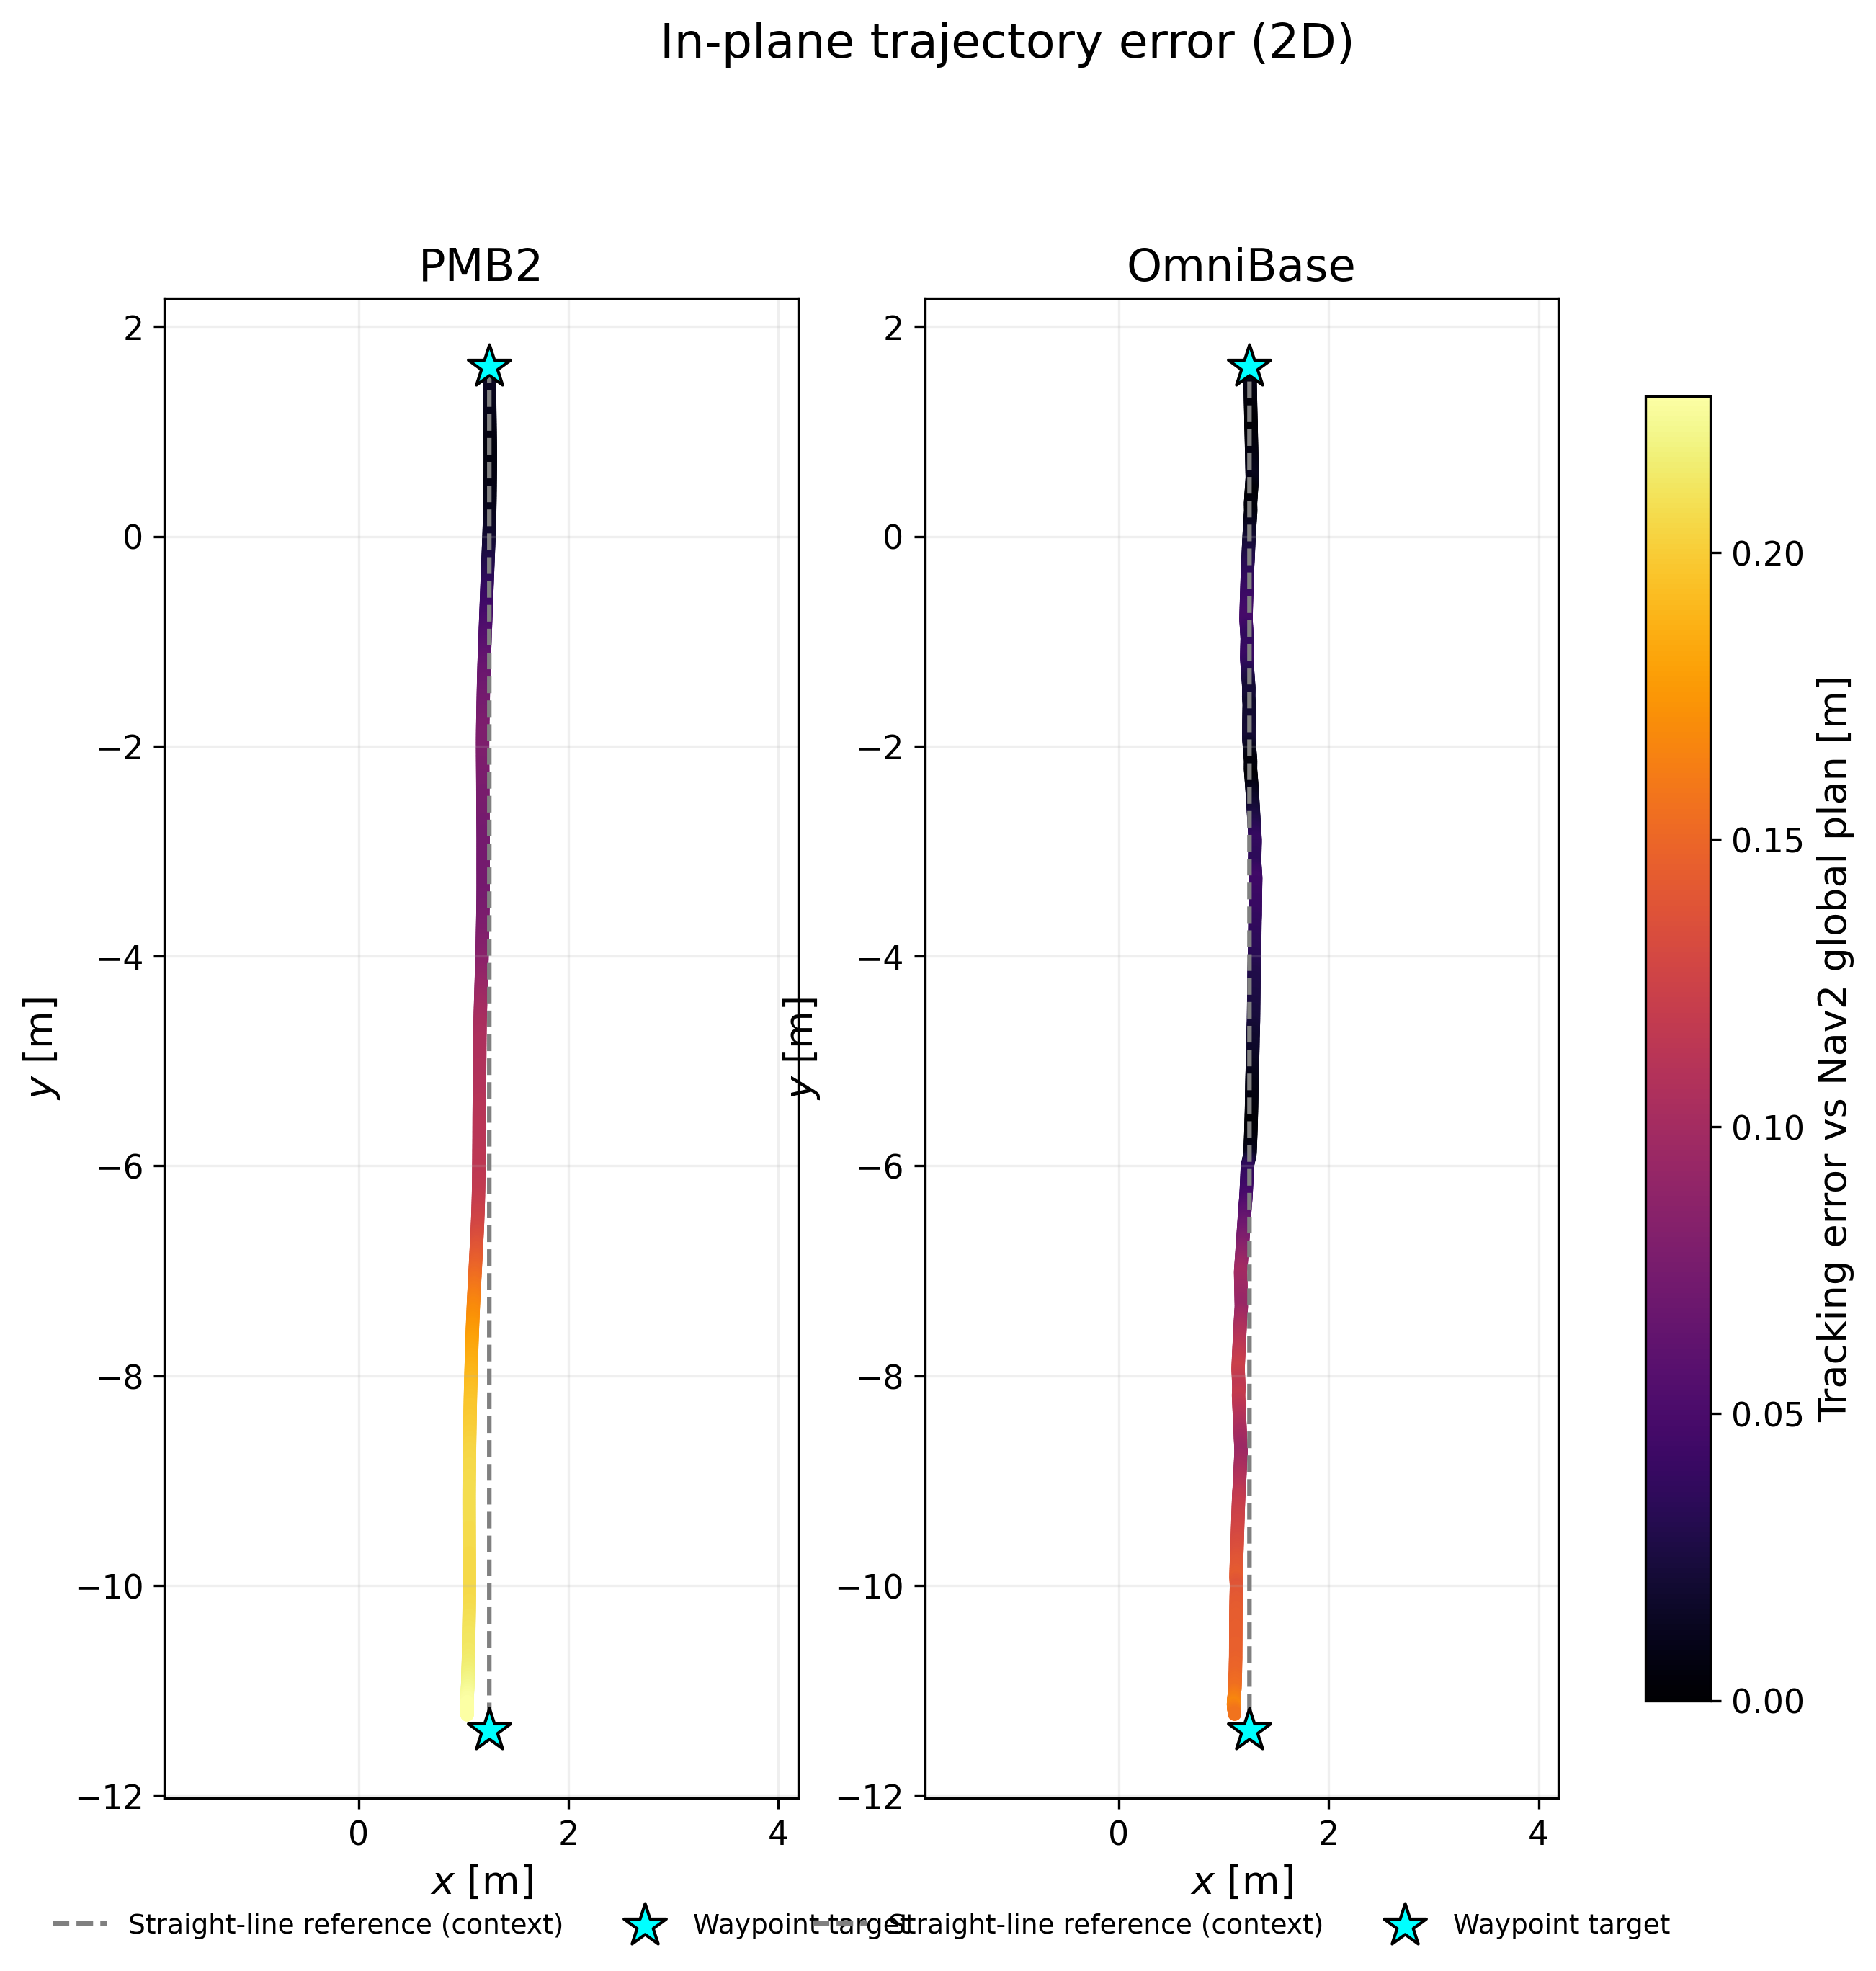
\includegraphics[width=\textwidth]{images/app_B/hallway_cross_track_error_2d.png}
  \caption{Straight corridor: in-plane tracking error (2D). The colour encodes the instantaneous deviation from the Nav2 global plan along the executed trajectory of the median run of each base; the drift accumulates towards the end of the corridor, more markedly for the differential PMB2.}
  \label{fig:app-2d-hallway}
\end{figure}

\begin{figure}[htbp]
  \centering
  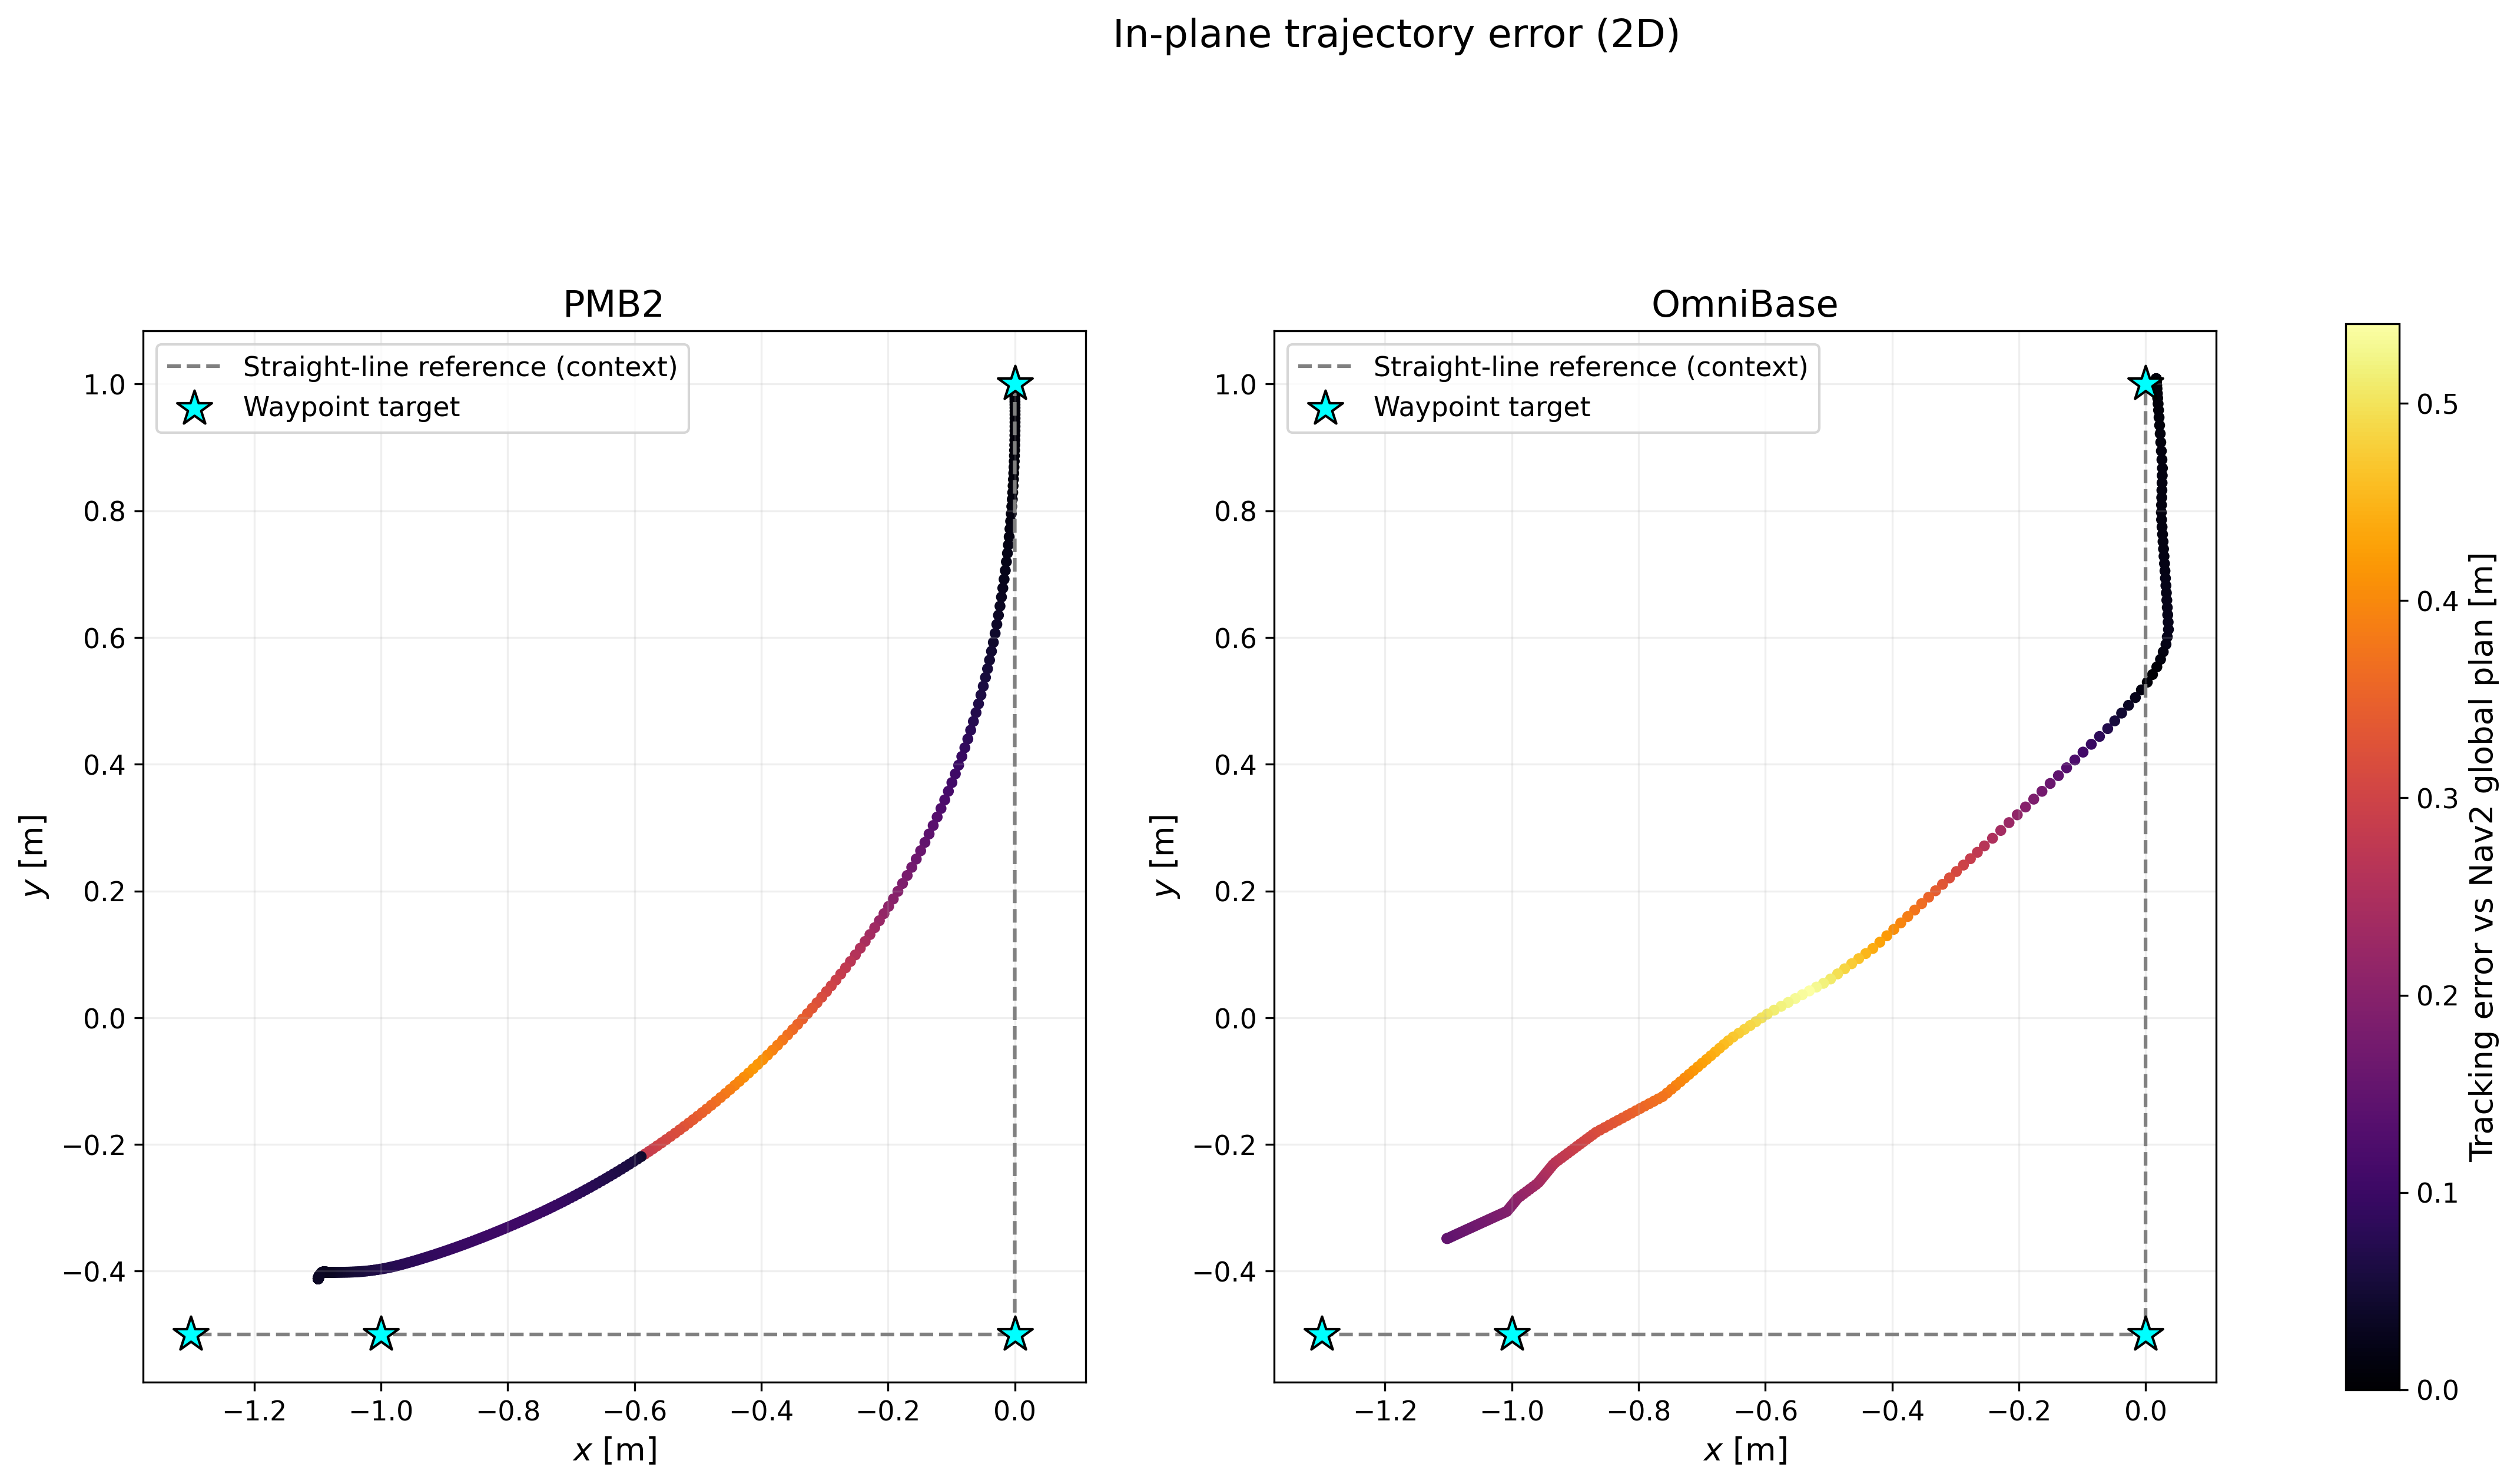
\includegraphics[width=\textwidth]{images/app_B/angle_cross_track_error_2d.png}
  \caption{Sharp corner: in-plane tracking error (2D). The largest deviation from the global plan occurs along the diagonal shortcut of the holonomic OmniBase, consistent with the aggregate values of Section~\ref{subsec:res-angle}.}
  \label{fig:app-2d-angle}
\end{figure}

\begin{figure}[htbp]
  \centering
  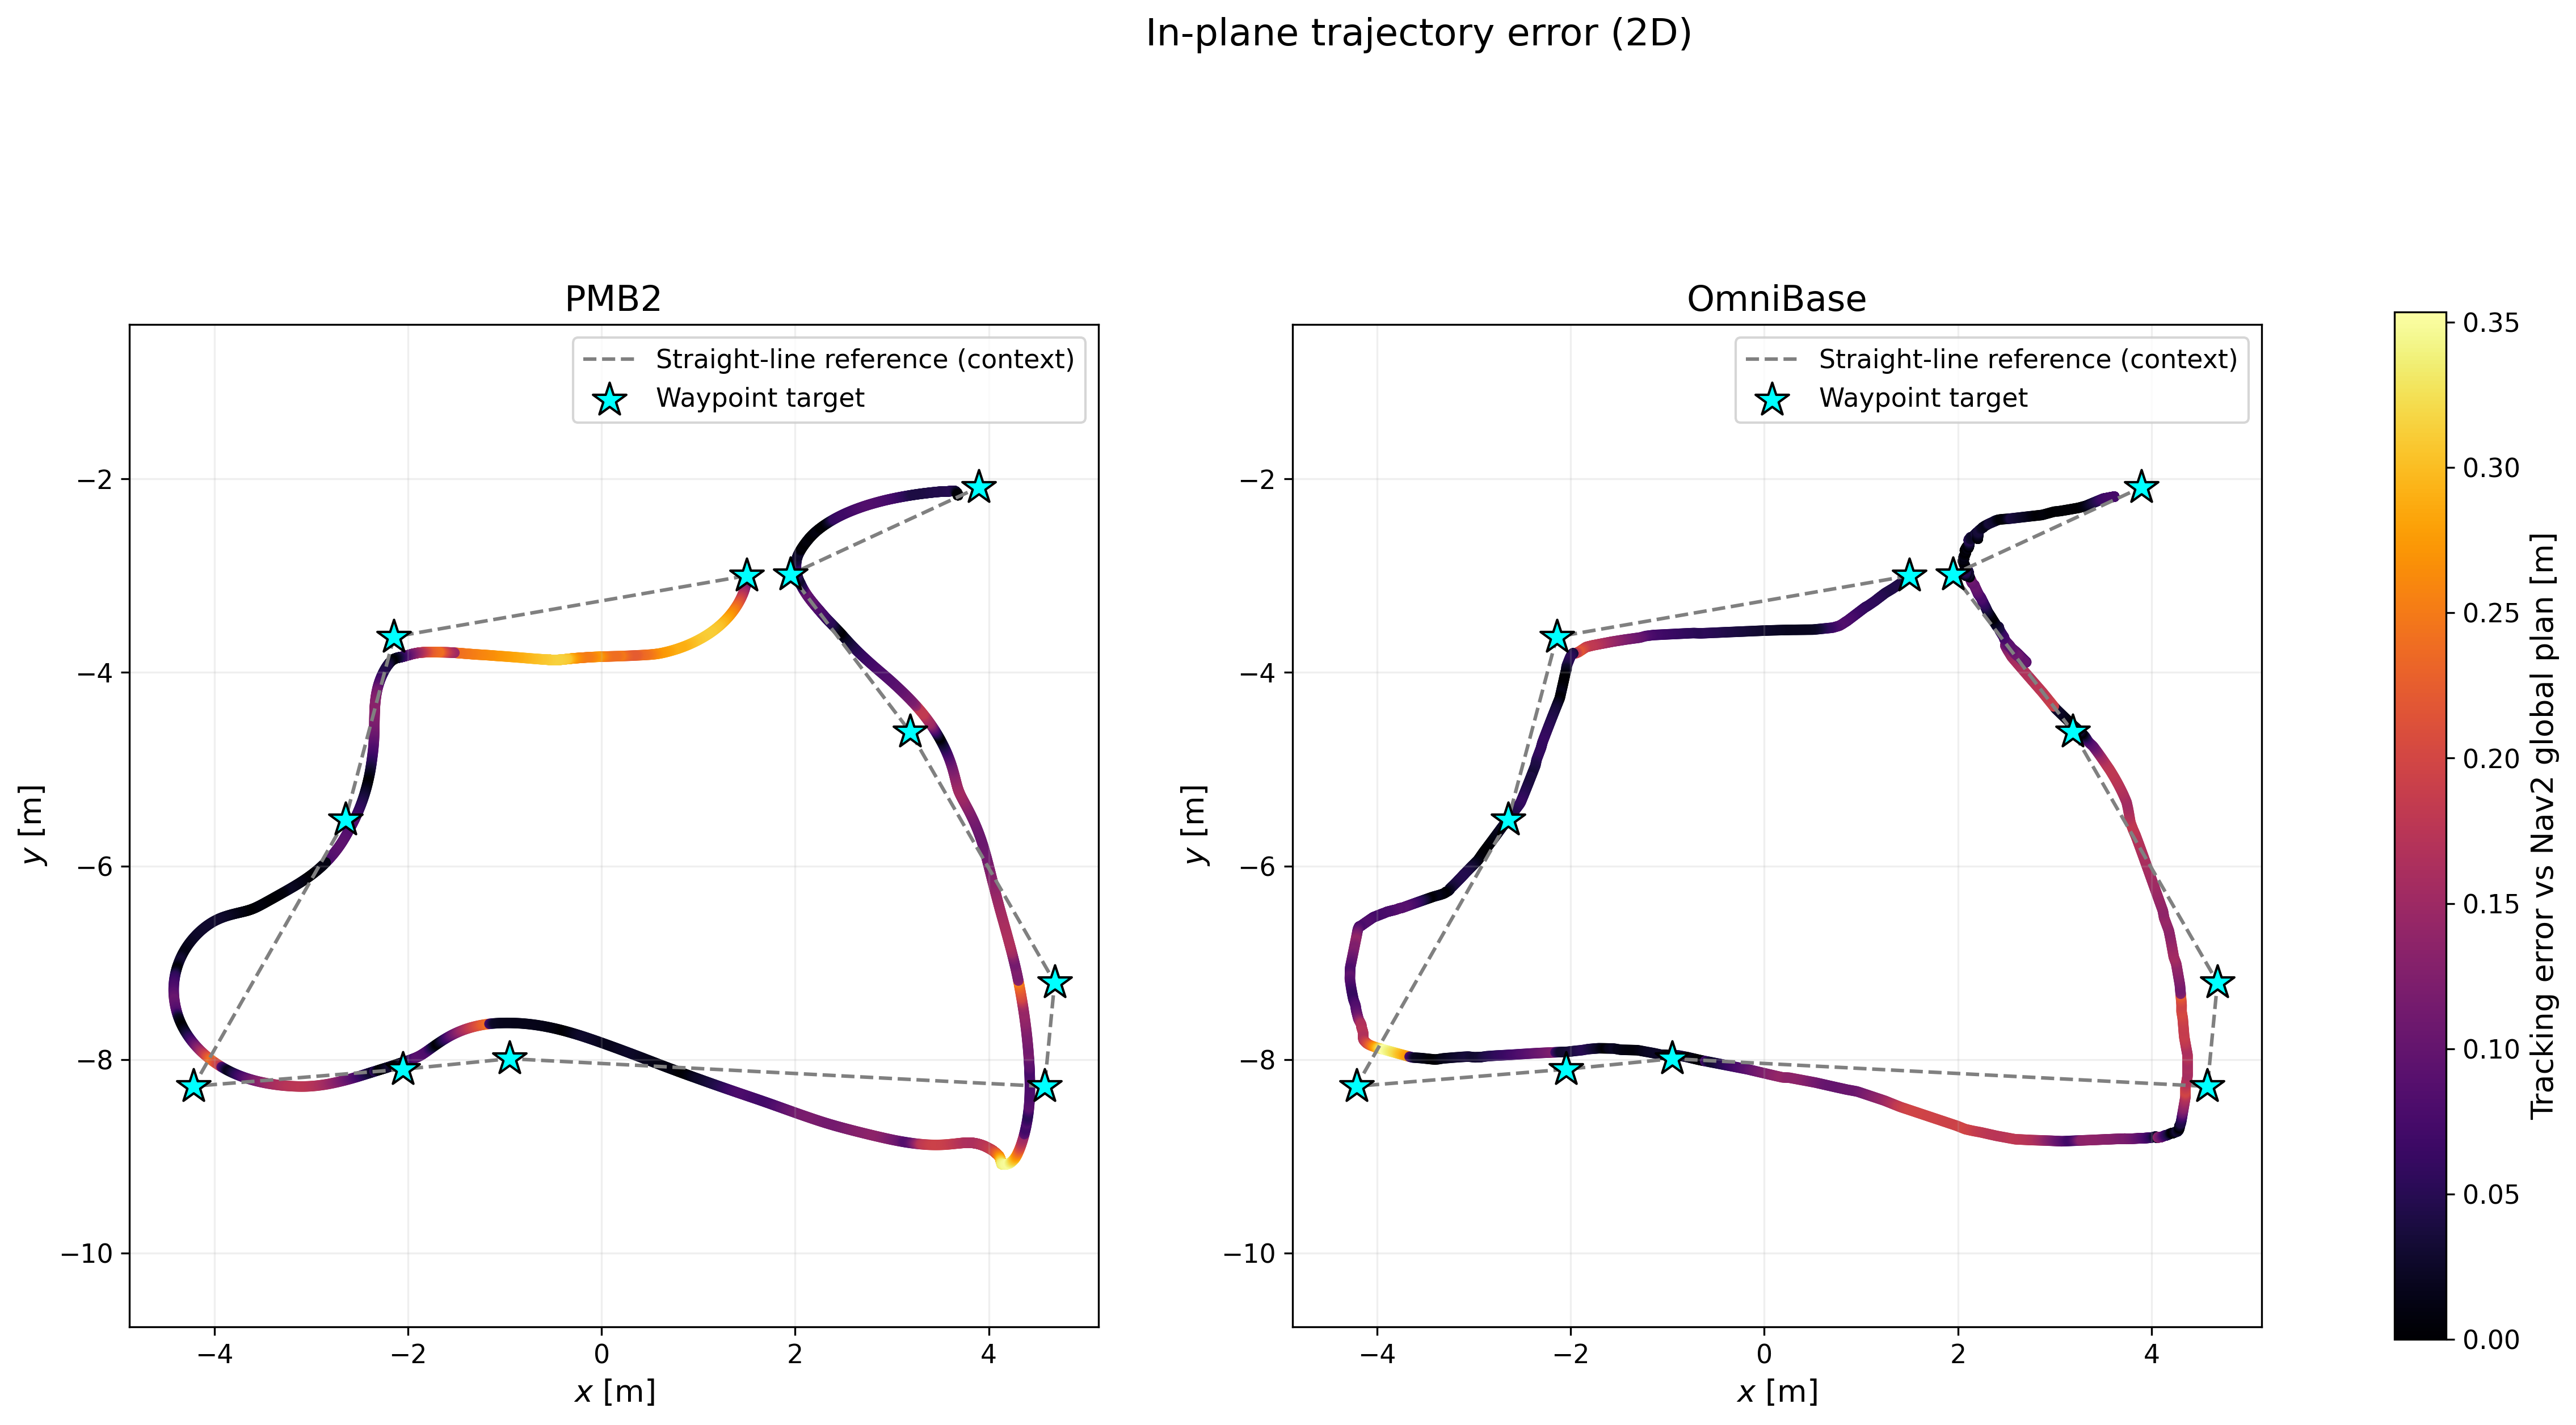
\includegraphics[width=\textwidth]{images/app_B/obs_cross_track_error_2d.png}
  \caption{Cluttered obstacle course: in-plane tracking error (2D). The deviation from the global plan is distributed along the whole circuit and peaks at the tight manoeuvres, remaining lower on average for the holonomic OmniBase.}
  \label{fig:app-2d-obs}
\end{figure}

\begin{figure}[t]
  \centering
  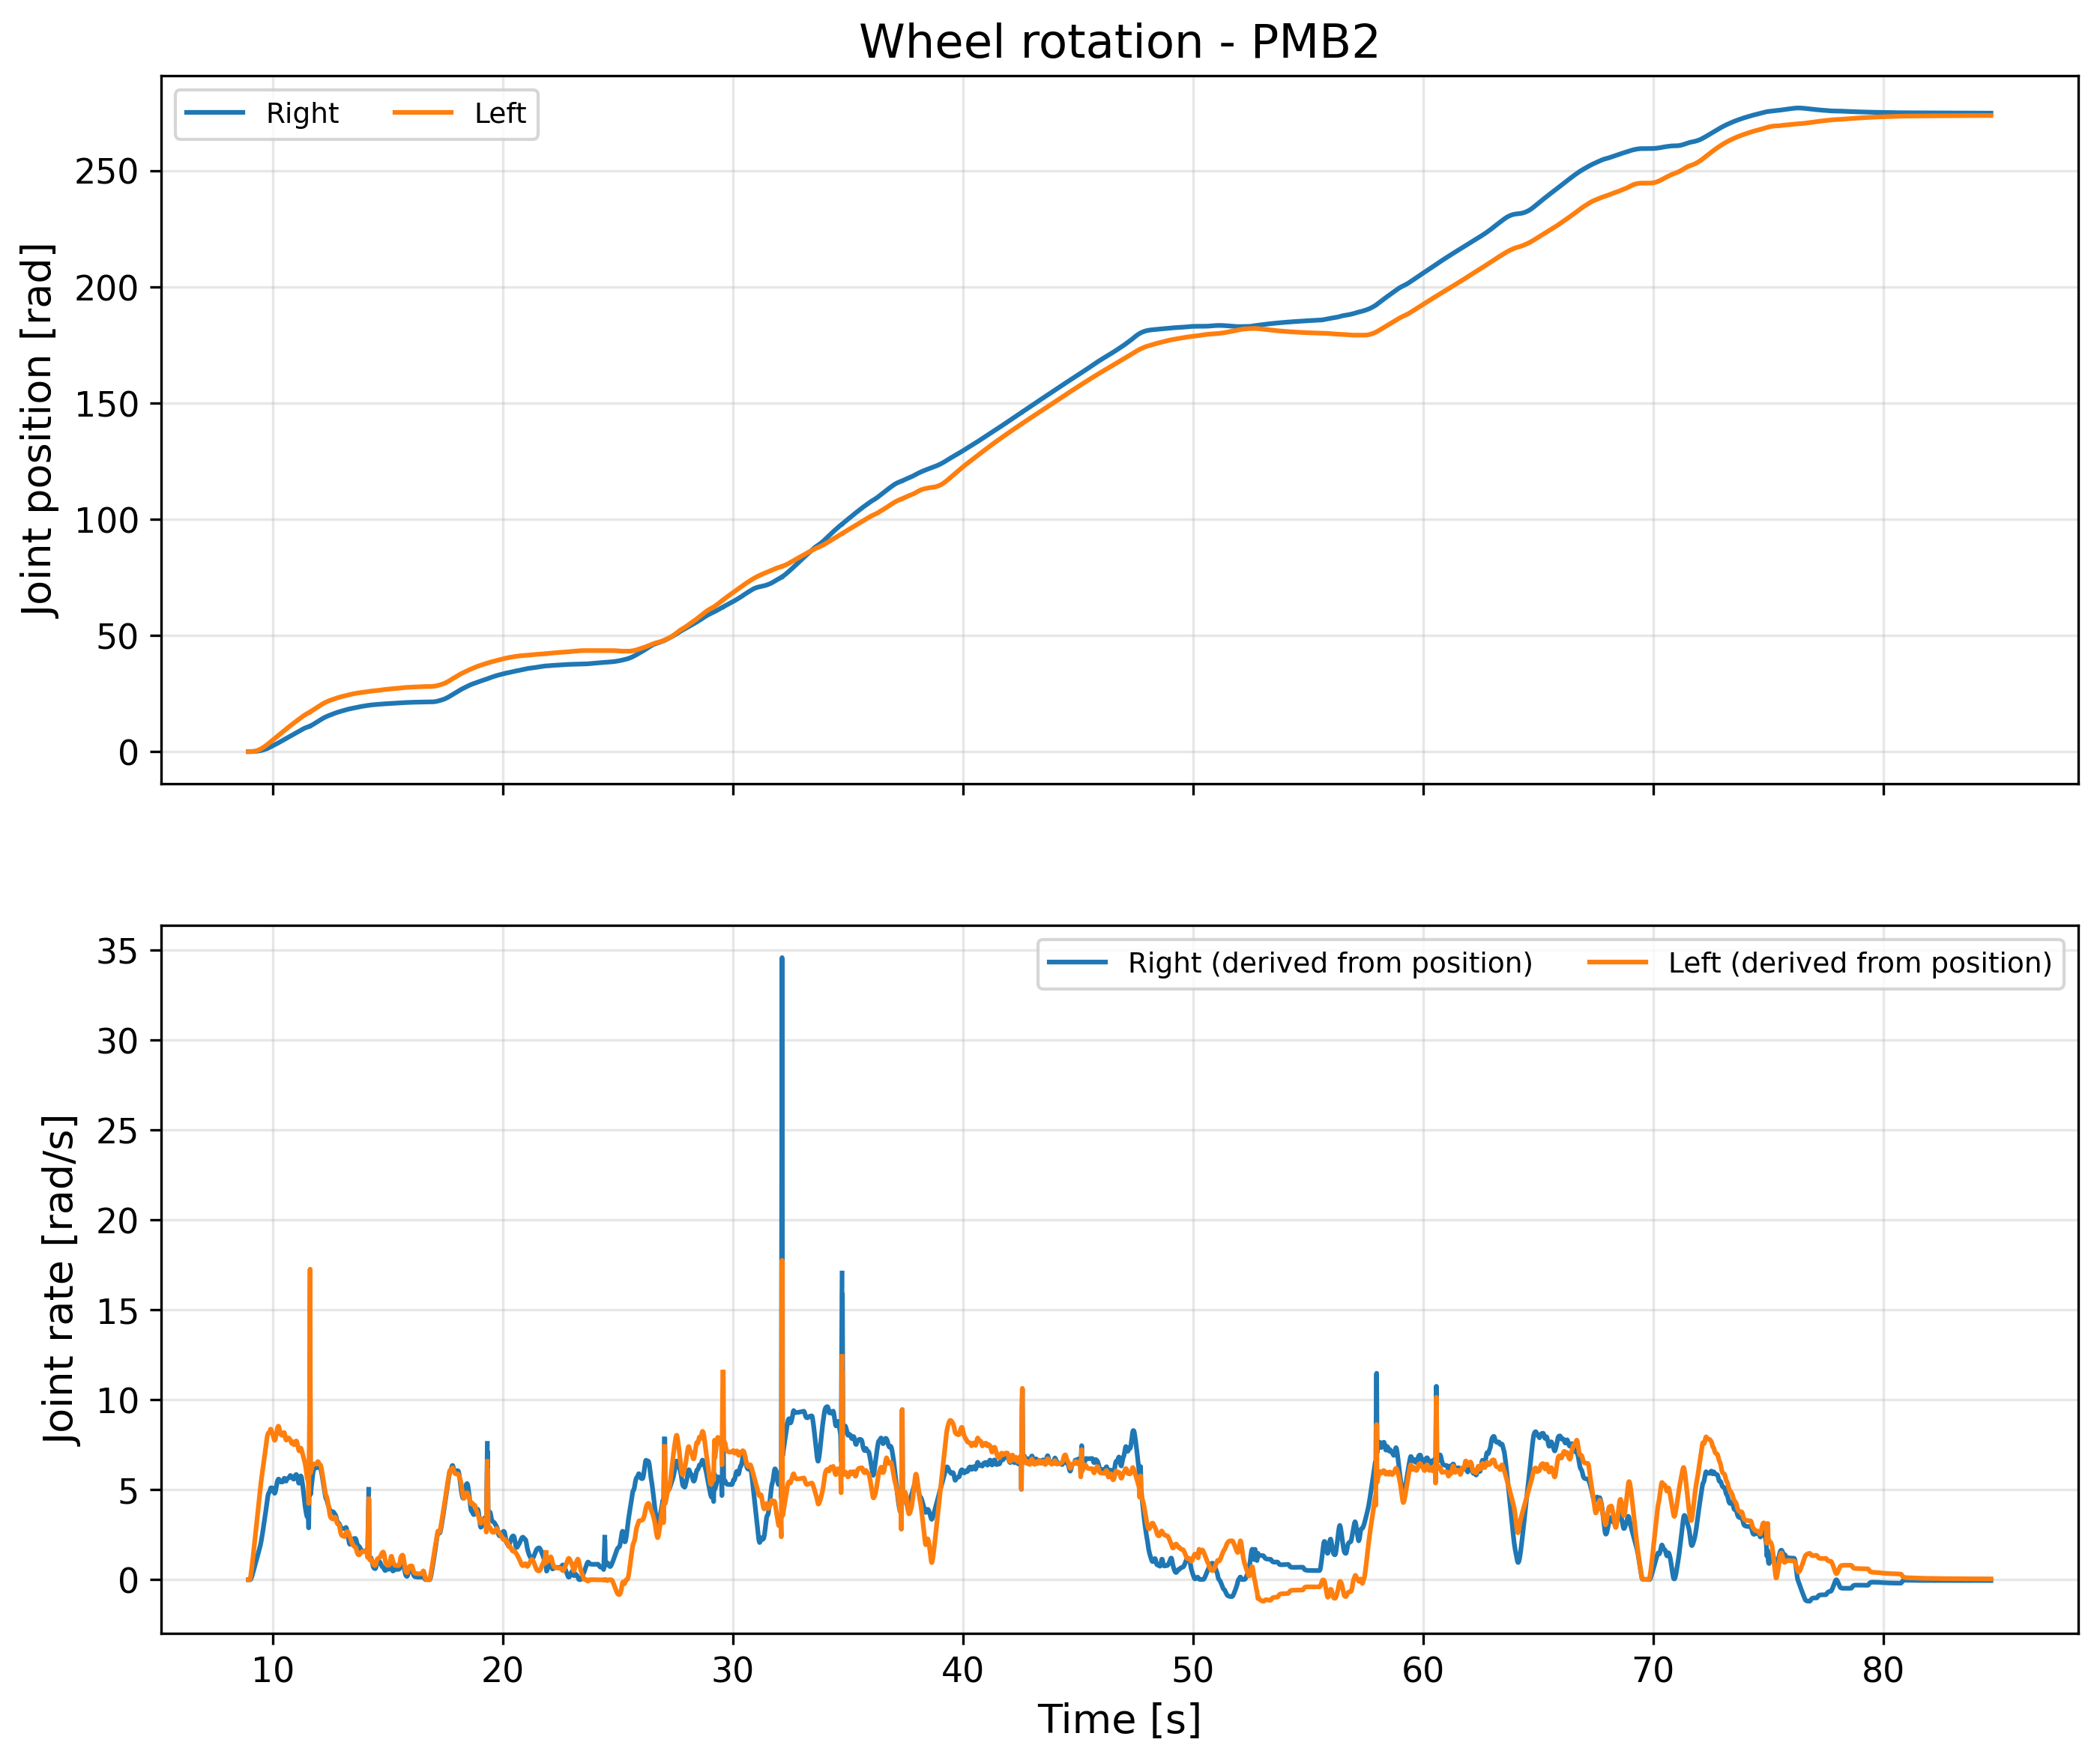
\includegraphics[width=\textwidth]{images/app_B/wheel_rotation_pmb2.png}
  \caption{Cluttered obstacle course: wheel rotation over time for the differential PMB2. In contrast to the straight corridor (Figure~\ref{fig:hallway-wheels-pmb2}), the frequent turns and manoeuvres produce strongly varying, repeatedly reversing wheel rotations.}
  \label{fig:app-wheels-obs-pmb2}
\end{figure}

\begin{figure}[t]
  \centering
  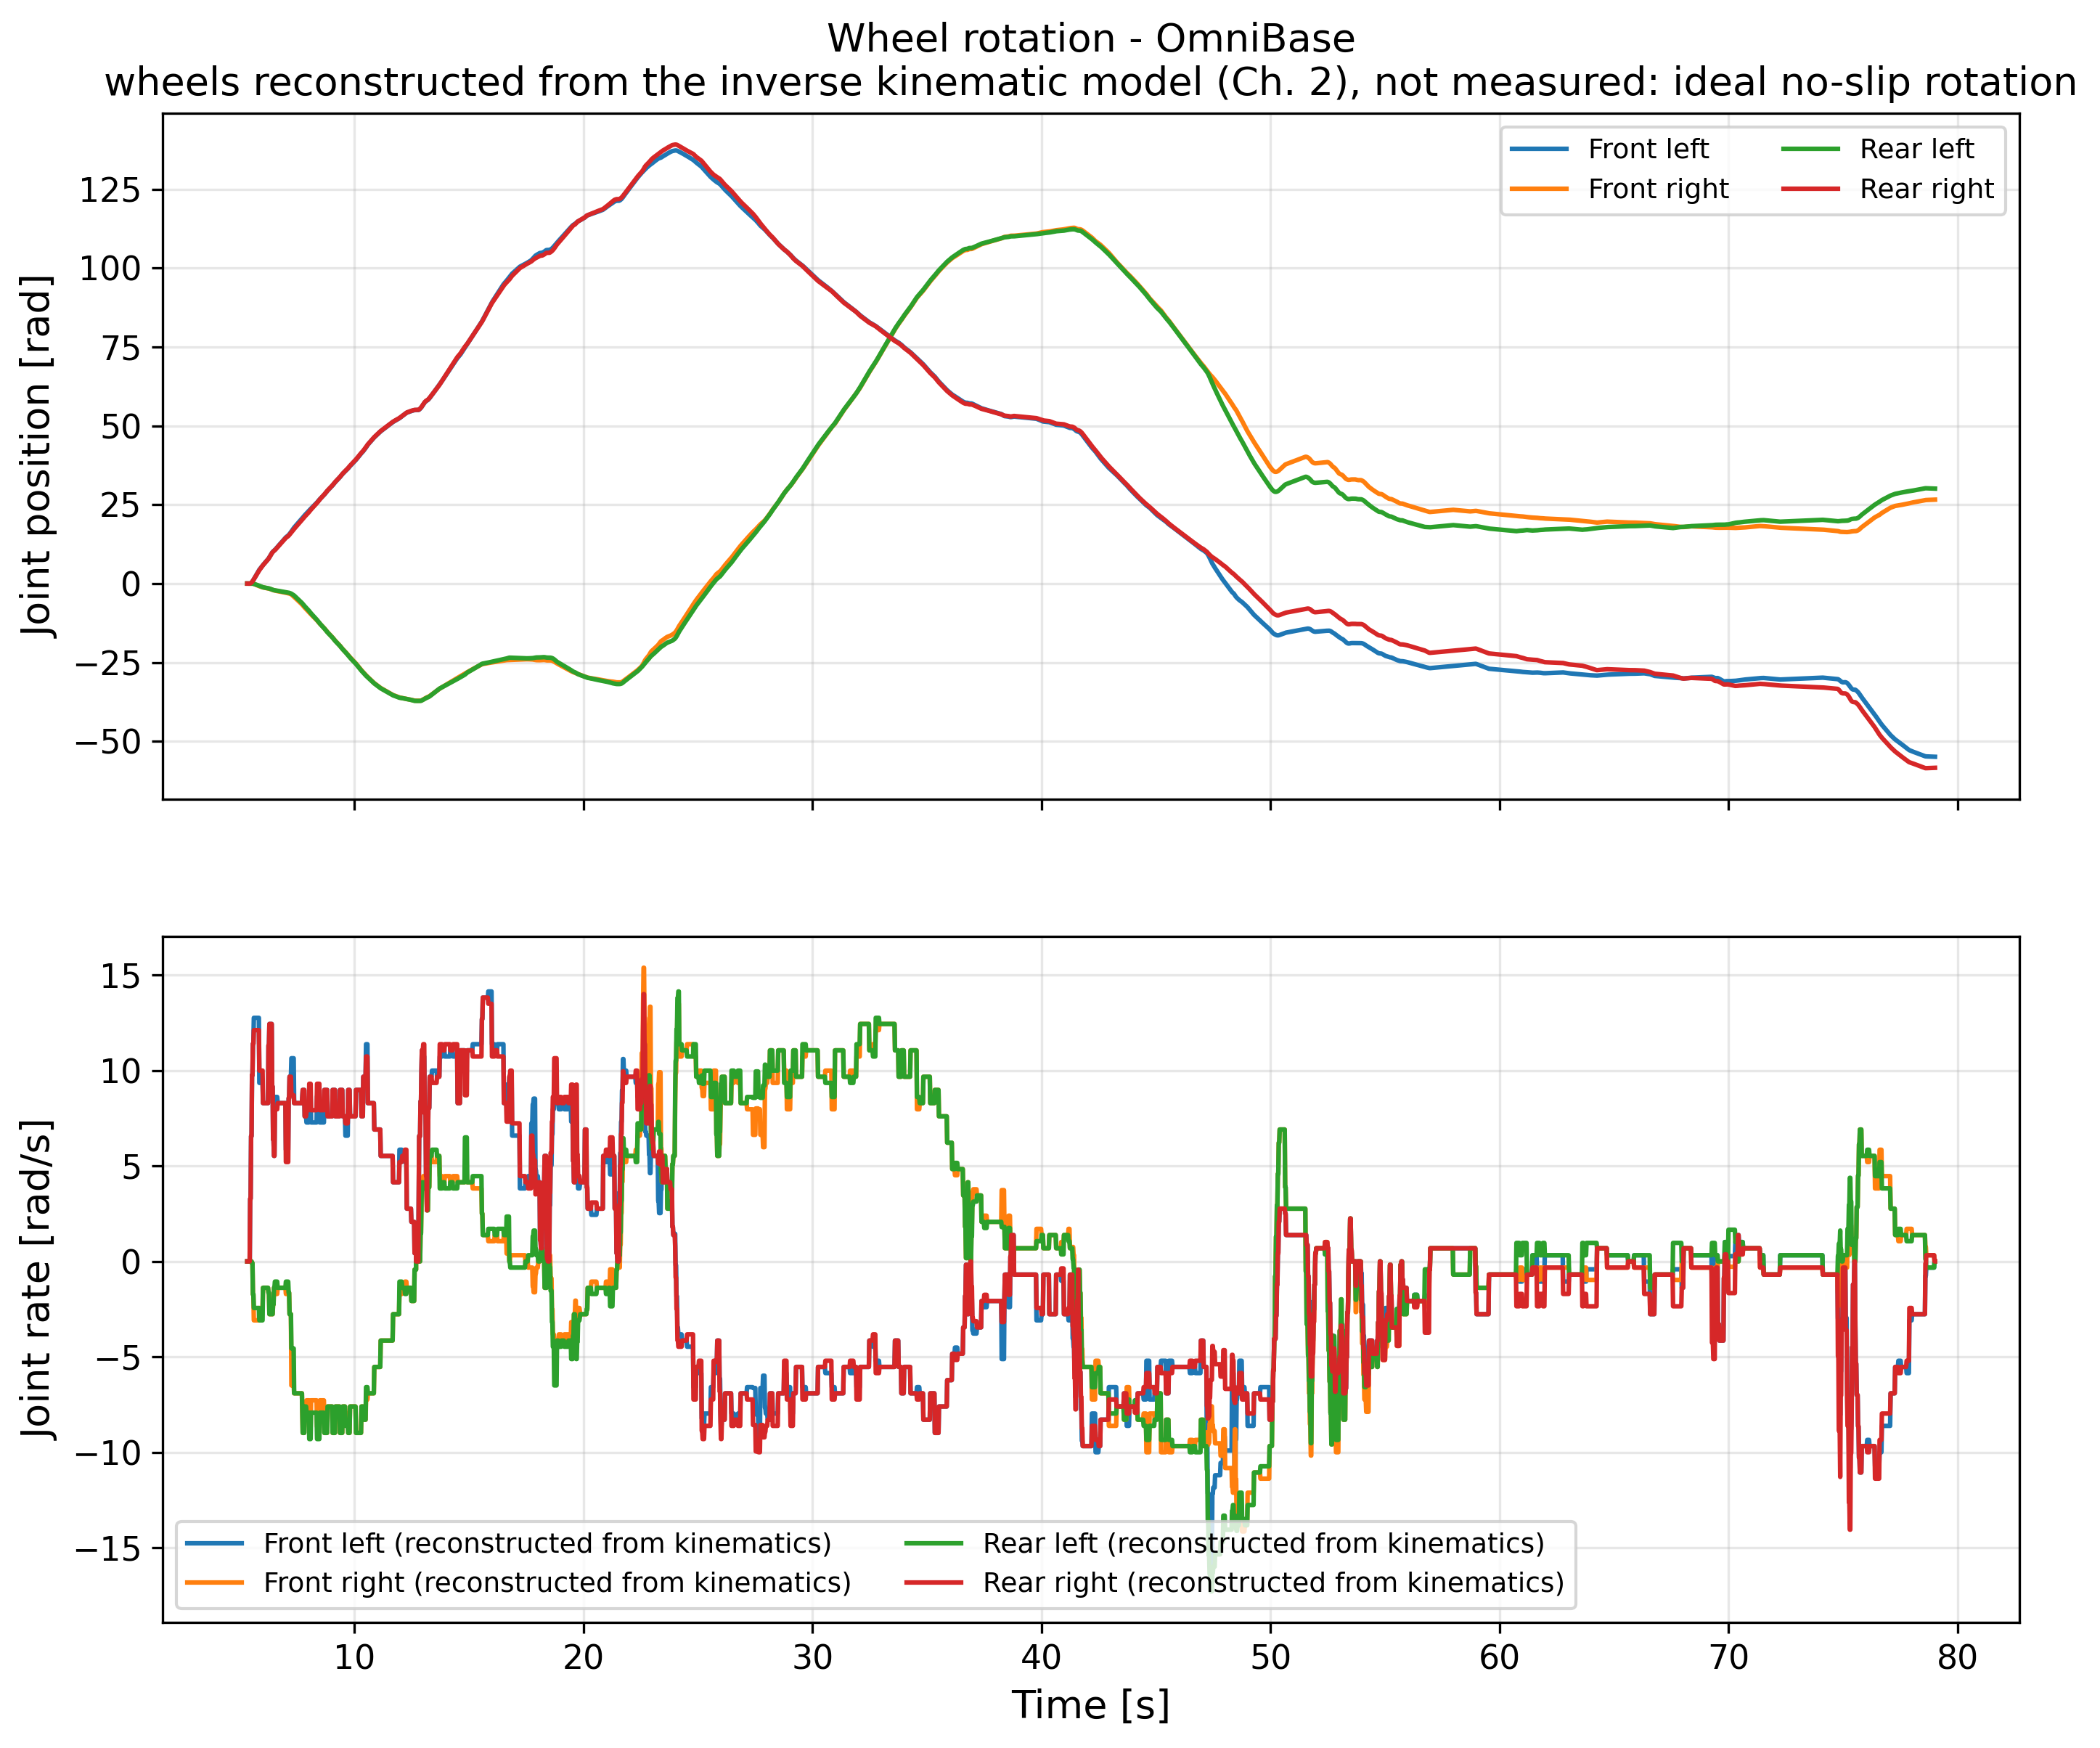
\includegraphics[width=\textwidth]{images/app_B/wheel_rotation_omni.png}
  \caption{Cluttered obstacle course: wheel rotation over time for the holonomic OmniBase, reconstructed from the inverse kinematic model of Chapter~\ref{Ch:Kinematic} (ideal no-slip rotation). The rich, frequently reversing profile reflects the combination of forward and lateral motion used to thread the cluttered circuit.}
  \label{fig:app-wheels-obs-omni}
\end{figure}

\begin{figure}[t!]
  \centering
  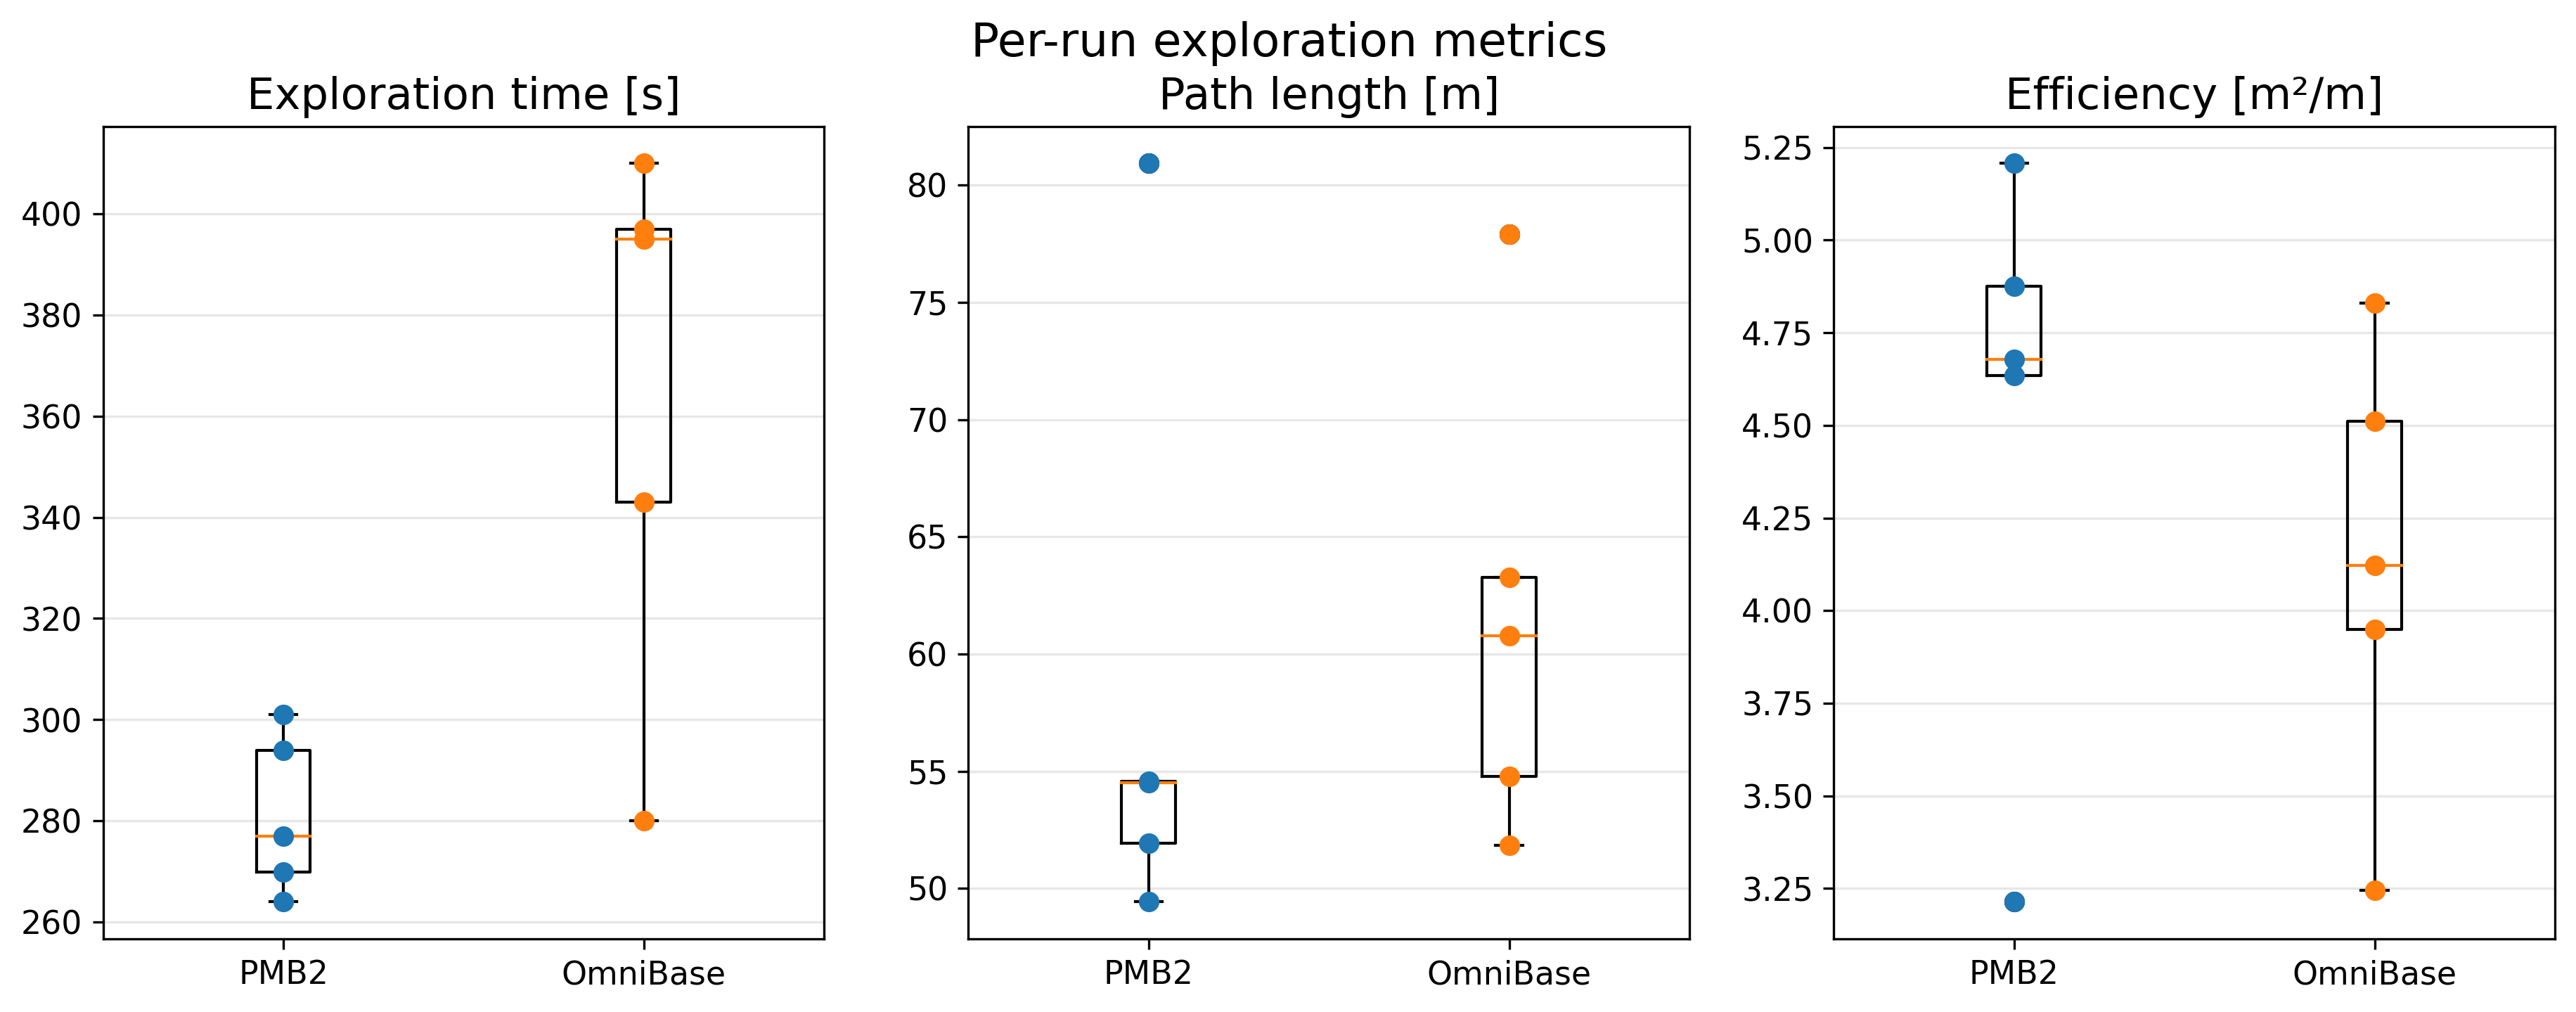
\includegraphics[width=\textwidth]{images/app_B/exploration_metrics_box.png}
  \caption{Autonomous exploration: per-run distribution of exploration time, path length, and area-per-metre efficiency. Complementing the aggregate values of Table~\ref{tab:explore}, the box plots expose the run-to-run spread hidden by the mean: the differential PMB2 is consistently faster and more efficient across its five runs, while the holonomic OmniBase shows a wider spread in both time and efficiency.}
  \label{fig:app-explore-box}
\end{figure}

% ==========================================
% BIBLIOGRAFIA
% ==========================================
\newpage
\printbibliography[heading=bibintoc, title={References}]
% ==========================================
% PAGINA VUOTA PER BELLEZZA E FIRME
% ==========================================
\clearpage
\thispagestyle{empty}
\null
\clearpage

\end{document}

